	\documentclass[10pt,oneside]{CBFT_book}
	
	% Paquetes que cargan
	
	\usepackage{standalone}
	\usepackage{amssymb}
	\usepackage{amsmath}
	\usepackage{graphicx}
% 	\usepackage{libertine}
% 	\usepackage[bold-style=TeX]{unicode-math}
	\usepackage{lipsum}

	\usepackage[numbers]{natbib}
	\setcitestyle{square}

	\usepackage{polyglossia}
	\setdefaultlanguage{spanish}
	
	\usepackage{CBFT.estilo} % Cargo la hoja de estilo
	
	\title{CURSO BÁSICO DE FÍSICA TEÓRICA}
	\subtitle{Volumen 4: Física Teórica 3 [Mecánica Estadística]}
	\author{E.F. Lavia}
	\date{\today}
	\version{versión 0.1}

	%###########################################################################
	%		DOCUMENTO 
	%###########################################################################
	
	\begin{document}
	\maketitle	
	
%	\pagenumbering{roman}
	\thispagestyle{empty}
	
	\tableofcontents
	
	\thispagestyle{empty}
	
	
% 	\listoffigures
	
% 	\listoftables

% 	\include{chaps/cft_prefacio}

	\clearpage

	%###########################################################################
	%		CAPITULOS DEL CURSO
	%###########################################################################
	
	\pagenumbering{arabic}
	
		\documentclass[10pt,oneside]{CBFT_book}
	% Algunos paquetes
	\usepackage{amssymb}
	\usepackage{amsmath}
	\usepackage{graphicx}
% 	\usepackage{libertine}
% 	\usepackage[bold-style=TeX]{unicode-math}
	\usepackage{lipsum}

	\usepackage{natbib}
	\setcitestyle{square}

	\usepackage{polyglossia}
	\setdefaultlanguage{spanish}
	



	\usepackage{CBFT.estilo} % Cargo la hoja de estilo

	% Tipografías
	% \setromanfont[Mapping=tex-text]{Linux Libertine O}
	% \setsansfont[Mapping=tex-text]{DejaVu Sans}
	% \setmonofont[Mapping=tex-text]{DejaVu Sans Mono}

	%===================================================================
	%	DOCUMENTO PROPIAMENTE DICHO
	%===================================================================

\begin{document}

% =================================================================================================
\chapter{Básicos de termodinámica}
% =================================================================================================

El que un cuerpo sea, a efectos termodinámicos, macroscópico o no dependerá de la relación entre las 
distancias características entre los componentes y el tamaño total teniendo en cuenta el potencial que 
hace interactuar a las partículas.
Así, por ejemplo, una galaxia no es un cuerpo macroscópico mientras que un barril de cerveza sí lo es.

El equilibrio termodinámica se da cuando macroscópicamente nada pasa en el sistema, aunque microscópicamente
siempre está sucediendo algo.

Una pared rígida y adiabática implica que no puedo interactuar con él; en cambio una pared rígida implica
solamente que no puedo interactuar por medios mecánicos [explicar].

El concepto de estado conlleva el desinterés por la manera en que llego a ese estado. Una variable 
termodinámica no puede depender de cómo el sistema llega a ese estados; por ello esa variable $F$ es un
diferencial exacto, es decir que
\[
	\oint dF = 0 \qquad \text{ y } \qquad F(b)-F(a) = \int_a^b dF
\]
implica que $F$ es variable de estado.

El gas ideal es tal que las partículas no interactúan entre sí. Es una aproximación de gases diluídos que
funciona bien a baja densidad.
Podemos expandir una expresión en términos de la densidad, lo cual se conoce como ecuación del virial.

Se busca hallar los coeficientes de dicha expansión a cada orden
\[
	p = \frac{nRT}{V}\left( 1 + \frac{n}{V} B(T) + \Frac{n}{V}^2 C(T) + ... \right)
\]
donde $B,C,...$ son los coeficientes del virial.
Van der Waals, según veremos después, es una primera corrección al gas ideal.

Se tiene el potencial de Lenard-Jones, que es de la forma $V \sim (x^{-12} - x^{-6} ) $

fig p1

En la ecuación de estado del gas ideal se tiene que todo el volumen es accesible todo el tiempo (el gas
puede ocupar todo el volumen).

Partículas no interactuantes (no tienen volumen)

En la expresión de Van der Waals,
\[
	p = \frac{nRT}{V - nb} - a \Frac{n}{V}^2
\]
el denominador del primer término tiene en cuenta el carozo, mientras que el segundo término tiene en
cuenta la disminución de presión (que es un efecto de las colas).

Al introducir la pared, a su derecha no hay partículas. Una del costado percibe el desbalance porque
desde el lado de la pared no hay partículas que le hagan fuerza.

fig p2 1

El desbalance hace que se frenen (es decir que tiendan a chocar menos contra la pared) y sientan por
ello menor presión (fuerza neta hacia adentro).

Las leyes de la termodinámica contienen toda la información.

% =================================================================================================
\section{Energía y entropía}
% =================================================================================================

Consideremos en primer lugar la energía; la aditividad de la energía.

Al seperar un sistema construyo una pared

fig p2 2

y si la energía era $E = E_1 + E_2 + H_{12}$ paso a considerar, al separarlos, que $E= E_1 + E_2$.
¿Bajo qué condición se da que $H_{12} \sim 0$ ? Para ello considero el potencial segundo

fig p2 3

La $E \geq V_0(\rho V)n_p$ el rango del potencial aceptará $1,2,...,i$ capas de vecinos. La primer capa
tendrá 6 vecinos. Si el potencial es gravitatorio interactúa con todos los vecinos, si su alcance es corto
interactuará con un número $i$ chico.

fig p2 4 y 5

El volumen de la interfase asociada al rango de interacción es $V'$. Entonces $ E_1 + E_2 $ con 
$H_{12} = V_0 \rho V n_p $.

Luego, si el rango de interacción es finito, entonces $H_{12} \sim 0$ y la energía es aditiva.
Si el rango de interacción no decae rápidamente entonces $H_{12} \neq 0$.
Se puede decir entonces que
\[
	E = E_1 + E_2 \qquad \Longleftrightarrow \qquad  \text{ El rango de la interacción es pequeño }
\]

La energía no es aditiva para sistemas coulombianos puros, gravitatorios o sistemas muy pequeños
porque allí el tamaño del sisistema es del orden de la interacción y no tiene sentido dividirlo.

El trabajo se puede escribir en general como
\[
	dW = p dV - J dL - \sigma dA - \vb{E}\cdot d\vb{P}
\]
\notamargen{$dW$ es un diferencial inexacto salvo en los casos en que el trabajo es adiabático.}
y además
\[
	\sum_{j} \mu_j dN_j \leftarrow \text{ Flujo de materia }
\]
La segunda ley de la termodinámica se enuncia en el siglo XVIII en el medio de la revolución industrial.
Aplicada a máquinas de vapor.

Una de las formulaciones de la 2da ley es definir la entropía. 
Surge de una escala de temperatura absoluta que emana desde
\[
	\frac{Q_1}{Q_2} = -\frac{T_1}{T_2} 
	\qquad \Rightarrow \qquad 
	\frac{Q_1}{Q_2} + \frac{T_1}{T_2} = 0 \quad
	\text{ reversible}
\]
que desemboca en la desigualdad de Clausius
\[
	\int \frac{dQ}{T} \leq 0.
\] 
De esto deducimos que $dQ/T$ es una diferencial exacta en el caso de sistemas reversibles.

\notamargen{$S$ será aditiva cuando $E$ sea aditiva.}

Proceso reversible en un sistema aislado
\[
	S_{A\to B} = \int_A^B dS = 0
\]
pues 
\[
	dS =\frac{dU}{T} - \frac{p}{V}dV + \frac{\mu}{T}dN = 0
\]
pero en procesos irreversibles la variación de $S$ es cota superior:
\notamargen{La existencia de $S$ es independiente de su cálculo}
\[
	\int_A^B \frac{dQ}{T} < \int_A^B dS = S_{A\to B}.
\]

Luego, para un sistema aislado, en un proceso irreversible 
\[
	dS_I = 0 \qquad \Rightarrow \qquad \frac{dQ_I}{T} = 0
\]
y entonces
\[
	0 < \int_A^B  dS =  S_{A\to B}
\]

La entropía solo aumenta. Podría calcular $S_{A\to B}$ con un proceso reversible de $A\to B$ pero ahí 
ya tengo que intervenir sobre el sistema (no hay procesos espontáneos --en un sistema aislado-- reversibles).

En reversibles
\[
	dU = TdS - pdV + \mu dN
\]
mientras que en irreversibles
\[
	dU = dQ_I - pdV +\mu dN, \quad \text{pero} \quad dQ_I < TdS 
\]
y entonces
\[
	dU < TdS - pdV + \mu dN
\]
% \begin{figure}[htb]
% 	\begin{center}
% 	\includegraphics[width=0.8\textwidth]{images/teo2_1.pdf}	 
% 	\end{center}
% 	\caption{}
% \end{figure} 
La entropía da un criterio para el equilibrio en sistemas aislados; el equilibrio es
equivalente al máximo de entropía.


\subsection{Funciones extensivas y homogéneas}

La entropía es extensiva y aditiva. 
Si $S$ es homogénea de primer orden de $U,V,N_j$ se tiene
\[
	S = S(\lambda U, \lambda X, \{\lambda N_i\}) = \lambda S( U, X, \{ N_i\})
\]
y además si \notamargen{En un sistema $PVT$ $Y=-p$.}
\[
	TdS = dU - YdX - \mu_i dN_i,
\]
donde $Y$ es una fuerza generalizada y $dX$ un desplazamiento generalizado,
\[
	\dtot{S}{\lambda} = S = \dpar{S}{\lambda U}\dtot{\lambda U}{\lambda} +
	\dpar{S}{\lambda X}\dtot{\lambda X}{\lambda} +
	\dpar{S}{\lambda N_i}\dtot{\lambda N_i}{\lambda}
\]
\[
	S = \dpar{S}{\lambda U} U + \dpar{S}{\lambda X} X + \dpar{S}{\lambda N_i} N_i
\]
\[
	\dpar{}{\lambda U}\left[ S(\lambda U)\right] = 
	\dpar{}{\lambda U}\left[ \lambda S( U)\right] = \dpar{S}{U} = \frac{1}{T}
\]
y procediendo del mismo modo con $Y,\mu$
\[
	S = \frac{1}{T} U + \frac{-Y}{T} X + \frac{-\mu_i}{T} N_i
\]
y arribamos a la ecuación fundamental
\[
	TS = U - YX - \mu_i N_i 
\]
o bien
\[
	U = TS + YX + \sum_i \mu_i N_i.
\]

\begin{ejemplo}{\bf Los mínimos de potencial y el equilibrio}

Considerando $W_{\text{libre}}$ un trabajo diferente del volumétrico, podemos poner
\[
	\Delta W = \int p dV + \Delta W_{\text{libre}}
\]
y $\Delta U$ se comporta como un reservorio donde guardo trabajo; de allí el concepto de potencial.
En un sistema con entropía constante $S$ tengo otro concepto de equilibrio
\[
	(\Delta H)_{{S,V,N}\text{rev}} = -  \Delta W_{\text{libre}}
\]
de modo que
\[
	(\Delta H)_{{S,V,N}} < -  \Delta W_{\text{libre}}
\]
Puedo pasar entre funciones de estado con la transformada de Legendre. Se puede demostrar que
transforma diferenciales exactas en diferenciales exactas y funciones homogéneas en
funciones homogéneas.
\[
	(\Delta H)_{S,N,Y} \geq 0 \quad 
	\text{ Es mínimo en el equilibrio, $H$ es la entalpía }
\]
\[
	(\Delta A)_{T,V,N} \geq 0 \quad 
	\text{ Es mínimo en el equilibrio, $A$ es la energía libre de Helmholtz }
\]
EL potencial $A$ es más {\it usable} que $H$ porque $T,V,N$ constantes son experimentalmente
más logrables.
\[
	(\Delta G)_{T,P,N} \geq 0 \quad 
	\text{ Es mínimo en el equilibrio, $G$ es la energía libre de Gibbs }
\]

Podemos resumir estos hechos, interesantes, en el siguiente cuadro

\begin{center}
\begin{tabular}{|c|c|c|}
\hline
$S$ & máximo & sistema aislado \\
$E$ & mínimo & $S,V,N$ \\
$H$ & mínimo & $S,P,N$ \\
$A$ & mínimo & $T,V,N$ \\
$G$ & mínimo & $T,P,N$ \\
\hline
\end{tabular}
\end{center}


\end{ejemplo}


La primera ley (en sistemas reversibles) era 
\[
	dU = TdS + YdX + \sum_i \mu_i dN_i
\]
y a $S,V,N$ constantes 
\[
	dU^R = 0 \qquad dU^I \leq 0
\]
la mínima $U$ es equilibrio.
Si existe trabajo que no es de volumen resulta 
\[
	dU < -dW_\text{libre}
\]
\[
	\frac{dQ}{dT} = \frac{dU}{T} + \frac{p}{T}dV - \frac{\mu}{T}dN = \frac{dQ}{dT} \leq dS
\]

Si el sistema está aislado será
\[
	0 \leq dS \quad \text{condición de equilibrio}
\]
alcanzando el máximo ya no puede disminuir la entropía.


% =================================================================================================
\section{Transformadas de Legendre de las funciones termodinámicas}
% =================================================================================================

\[
	f(x,y,z) \qquad \text{con pendientes} \quad \dpar{f}{x},\dpar{f}{y},\dpar{f}{z}
\]
entonces 
\[
	\varphi(f_x,y,z) = f(x,y,z) - \left. x \dpar{f(x,y,z)}{x}\right|_{y,z}
\]
es la transformada de Legendre respecto de $x$, mientras que 
\[
	\varphi(f_x,f_y,z) = f(x,y,z) - x \dpar{f}{x} - y \dpar{f}{y}
\]
es la transformada de Legendre respecto de $y$.

La transformada de Legendre transforma una función homogénea en otra función homogénea, mantiene el
carácter de función de estado.
\[
	d\varphi(f_x,y,z) = df - dx \dpar{f}{x} - x d\left( \dpar{f}{y} \right)
\]

Para el caso de la energía
\[
	U=U(S,V,N) \qquad \qquad dU = TdS - pdV + \mu dN
\]
y entonces
\[
	A = U - \left. S\dpar{U}{S}\right|_{V,N} = U - ST \qquad \Rightarrow \qquad  A=A(T,V,N)
\]
\[
	H = U - \left. V\dpar{U}{V}\right|_{S,N} = U + pV \qquad \Rightarrow \qquad  H=H(S,p,N)
\]
\[
	G = U - \left. S\dpar{U}{S}\right|_{V,N} - \left. V\dpar{U}{V}\right|_{S,N} = 
	U - ST + pV \qquad \Rightarrow \qquad  G=G(T,p,N)
\]
\[
	dA = dU - SdT - TdS = -SdT - pdV + \mu dN
\]
\[
	dA \leq -SdT - pdV + \mu dN 
\]
entonces $A$ mínimo es equilibrio a $T,V,N$ constantes.

La idea de las transformadasd de Legendre es pasar la dependencia de cierto juego de variables a otro
que podría ser más apropiado par el sistema en cuestión.

Sistema aislado en equilibrio, entonces se tendrá $S$ máxima y como $S(U,V,N)$ y considero fluctuación
energética
\[
	\left. \dpar{S}{U} \right|_{\text{eq}} = 0 \qquad \left. \dpar2{S}{U} \right|_{\text{eq}} < 0
\]
\[
	\delta S_{\mathrm{orden 2}} = \frac{1}{2} \left. \dpar2{S}{U} \right|_{\text{eq}} \delta U^2
\]

% =================================================================================================
\section{Introducción a algunas ideas}
% =================================================================================================

Lo que sigue parece ser un enfoque de la termodinámica, más formal, siguiendo el libro de H.B. Callen (que
es un libro recomendado)

Consideramos esto como un sistema macroscópico; de la mecánica podemos ver que se moverá en modos
normales.

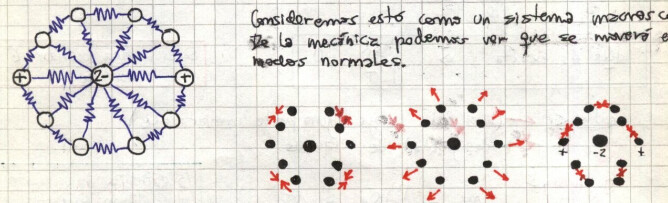
\includegraphics[width=0.80\textwidth]{images/1606329005.jpg}

Consideramos: 1) variables ocultas, 2) variables mecánicas y 3) variables eléctricas.
En una descripción promedio 1) no lo percibo, pero 2) sí porque incluye cambios en volumen y 3) lo veré
porque varía el momento dipolar eléctrico.
No puedo medir estos modos pero sí verlos macroscópicamente.

Las variables ocultas estarán asociadas a una energía interna
\[
	W = \Delta K + \Delta P_0
\]
\[
	W + q = \Delta K + \Delta P_0 + \Delta U
\]
donde $q$ está asociado a los grados de libertad ocultos. En termodinámica, no trataremos de las formas de 
energía macroscópicas (cinética y potencial). Considero el cuerpo fijo en el centro de masas, etc. y me
preocupo solamente de la energía interna
\[
	W + Q = \Delta U
\]
de modo que entonces, considerando $\delta W$ un diferencial inexacto se puede escribir
\[
	\delta W = - p dV + J d\ell + \sigma dA + E dP
	+ H dM + \phi de + \sum_{i} \: \mu_i dN_i
\]
El primer término es el trabajo mecánico, el segundo y tercero son el trabajo de longitud y de superficie,
respectivamente, que multiplican un diferencial de longitud y área por la tensión lineal $J$ y la tensión
superficial $\sigma$. Luego el cuarto y quinto términos son los trabajos de variación del momento dipolar
y magnético, mientras que el sexto es el trabajo asociado a la electrostática y finalmente la sumatoria
contempla el trabajo para variar el número de partículas de una especie siendo $\mu_i$ el potencial químico
asociado a la especie $i$-ésima.

El trabajo siempre es producto de una variable extensiva por una intensiva (son conjugadas una de otra).
En general
\[
	\delta W = Y dX
\]
donde $Y$ es una fuerza generalizada (intensiva) y $dX$ es un desplazamiento generalizado (extensivo).

Se puede construir la termodinámica sobre los hombros de cuatro postulados.
\begin{enumerate}
 \item Se postula la existencia de estados de equilibrio caracterizados por 
 \[
	U, V, N_1, ..., N_r \qquad \text{ ($r$ especies) }
 \]
 \item Existe una función llamada entropía $S$ con
 \[
	S = S(U, V, N_1, ..., N_r)
 \]
 definida para los estados de equilibrio. Los valores que toman los parámetros extensivos en
 ausencia de ligaduras internas son aquellos que maximizan la entropía.
 \item La entropía es aditiva, continua y diferenciable y además es una función creciente de la
 energía interna
 \[
	\dpare{S}{U}{V,N} > 0,
 \]
 de aquí saldrá el hecho de que $T > 0$ (las temperaturas serán definidas positivas).
 Entonces, en un sistema compuesto
 
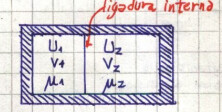
\includegraphics[width=0.30\textwidth]{images/1606329014.jpg}
 
 se tiene 
 \[
	S = S_1 + S_2 \qquad \qquad S = S_1(U_1,V_1,\mu_1) + S_2(U_2,V_2,\mu_2)
 \]
 de modo que si se retira la ligadura interna el sistema se equilibrará variando las entropías $S_1,S_2$
 maximizando $S$. Las variables $U_i,V_i,\mu_i$ se acomodan para hacer $S$ máxima.
 \item Cuando la entropía sea nula se tiene
 \[
	\dpare{S}{U}{V,N} = 0,
 \]
 lo cual es equivalente al tercer principio.
\end{enumerate}

Como consecuencia de la aditividad se tiene
\[
	S(\lambda U, \lambda V, \lambda N_1, ..., \lambda N_r ) =
	\lambda S(U,V,N_1,...,N_r),
\]
es decir que $S$ es homogénea de grado 1, lo cual sobreviene de haberle pedido por postulado dicha
característica. Se puede pasar de $S(U,V,N)$ a $U(S,V,N)$ que es la ecuación fundamental.
Luego, obtengo todo lo demás utilizando los postulados.

La energía en $U(T,V,N)$ no es fundamental porque no involucra cantidades extensivas; la definición
de $S$ anterior involucra cantidades extensivas, no intensivas.
Una variación a primer orden de $U$ resulta en
\[
	dU = \dpare{U}{S}{V,N} \: dS + \dpare{U}{V}{S,N} \: dV + \dpare{U}{N}{S,V} \: dN
\]
donde las derivadas parciales son, respectivamente, $T,-p$ y $\mu$ (consideramos una única especie).

Estas derivadas parciales serán intensivas. Regularán el intercambio de cantidades extensivas.
La temperatura $T$ está asociada al intercambio de entropía respecto a cierta variación de energía.
Entonces,
\[
	dU = TdS - p dV + \mu dN
\]
y solo para estados de equilibrio se tiene $dU = \delta Q + \delta W$ donde $\delta Q = T dS$ (recordemos
que $S$ está definida para estados de equilibrio).

\begin{ejemplo}{\bf Problema}
 
\end{ejemplo}



% =================================================================================================
\section{Gas de Van der Waals}
% =================================================================================================

Van der Waals incorpora la interacción molecular. \notamargen{Esta subsección tiene cinco gráficos}
\[
	\left( p +\frac{an^2}{V^2} \right)(V- nb) = nRT
\]
donde $a,b(T)$ caracterizan al gas en cuestión.

La función $p=p(V)$ tiene tres extremos para $T<T_c$,
\[
	\dpar{p}{V} = 0
\]
En $T=T_c$ es
\[
	\left.\dpar{p}{V} \right|_{T_c} = 0 \qquad \left.\dpar[2]{p}{V} \right|_{T_c} = 0
\]
punto de inflexión
\[
	v_c = 3b \qquad p_c = \frac{a}{27b^2} \qquad T_c = \frac{8a}{27Rb}
\]
y eso lleva a la ley de estados correspondientes
\[
	\left( \bar{p} + \frac{3}{\bar{v}^2} \right)(3 \bar{v} - 1)= 8\bar{T}
\]

De Van der Waals al virial
\[
	p = \frac{nRT}{(V-nb)} - a \left(\frac{n}{V} \right)^2 = 
	\frac{nRT}{V(1-b/v)}- \frac{a}{v^2}
\]
\[
	p = \frac{RT}{v}\left[ 1 + \frac{b}{v} - \frac{a}{vRT} \right] =
	p = \frac{RT}{v}\left[ 1 + \frac{1}{v}\left( b - \frac{a}{RT} \right) \right]
\]
y el último paréntesis es el primer coeficiente del virial.

Un potencial intermolecular está compuesto de una zona repulsiva (carozo duro) y una atractiva (cola)
\[
	V_{eff} = V-b \qquad (\mathrm{menor volumen por el carozo})
\]
\[
	p = \frac{RT}{V-b} - \left(\frac{a}{V}\right)^2 \qquad (\mathrm{menor presión por la atractividad})
\]
y entonces, por mol de sustancia,
\[
	\left( p +\frac{a^2}{V^2} \right)(V- b)= RT
\]

$b$ corrige el volumen que es ahora menor porque las partículas ocupan espacio. $a$ corrige la presión dado que la 
atracción tiende a formar pares bajando la presión sobre las paredes.

Las funciones respuesta tienen signo errado dentro de la zona del rulo\notamargen{Recordemos que
\[ -\frac{1}{v}\dpar{v}{p}=\kappa_T > 0\]}
\[
	\dpar{p}{V}>0 \rightarrow  \dpar{v}{p} >0 \Rightarrow \kappa_T < 0 \qquad (\mathrm{MAL})
\]
\[
	dT = -SdT + VdP + \mu dN
\]
dada la isoterma y que $N$ es constante 
\[
	dG = Vdp \rightarrow dg = v dP \quad (\mathrm{molar})
\]
$G$ es cóncava en $p$ entonces 
\[
	v = \left.\dpar{g}{p} \right|_{T,N}, \qquad  
	\dpar{v}{p} =\left.\dpar[2]{g}{p} \right|_{T,N} < 0
\]
y luego 
\[
	\Delta g = \int_{p_c}^{p_G} v dp = 0
\]
entonces 
\[
	\int_C^D + \int_D^E + \int_E^F + \int_F^G = 0
\]
y si se invierten puntos para tener un recorrido según las flechas se llega a 
\[
	\int_C^D - \int_E^D = \int_F^E - \int_F^G 
\]

Áreas inguales determinan entonces los puntos C y G de forma que se corrige Van Der Waals para dar curvaturas
correctas. En la región de coexistencia hemos trocado
\[
	\dpar{p}{V} > 0 \quad \mathrm{por} \quad \dpar{p}{V}=0
\]
lo cual da $\kappa_T \to \infty$ en lugar del $\kappa_T < 0$ (que es incorrecto).









% \bibliographystyle{CBFT-apa-good}	% (uses file "apa-good.bst")
% \bibliography{CBFT.Referencias} % La base de datos bibliográfica

\end{document}

	
		\documentclass[10pt,oneside]{CBFT_book}
	% Algunos paquetes
	\usepackage{amssymb}
	\usepackage{amsmath}
	\usepackage{graphicx}
% 	\usepackage{libertine}
% 	\usepackage[bold-style=TeX]{unicode-math}
	\usepackage{lipsum}

	\usepackage{natbib}
	\setcitestyle{square}

	\usepackage{polyglossia}
	\setdefaultlanguage{spanish}
	



	\usepackage{CBFT.estilo} % Cargo la hoja de estilo

	% Tipografías
	% \setromanfont[Mapping=tex-text]{Linux Libertine O}
	% \setsansfont[Mapping=tex-text]{DejaVu Sans}
	% \setmonofont[Mapping=tex-text]{DejaVu Sans Mono}

	%===================================================================
	%	DOCUMENTO PROPIAMENTE DICHO
	%===================================================================

\begin{document}

% =================================================================================================
\chapter{Conjuntos estadísticos}
% =================================================================================================


\section{Mecánica estadística. Boltzmann y teoría cinética}

Estaremos pensando en un hamiltoniano para muchas partículas (dinámica real)
\[
	H = \sum_i \frac{p^2}{2m} + \sum_{i < j} v_{ij}(|v_i-v_j|) + \sum_i U_i
\]

Sistema diluido. Las colisiones a un tiempo fijo son entre dos partículas; no entre más.
También lo garantiza esto la forma del potencial que se esfuma rápidamente a gran distancia.
Los procesos colisionales se definirán en base a $\sigma$, la sección eficaz, que no es otra cosa
que una probabilidad de transición.

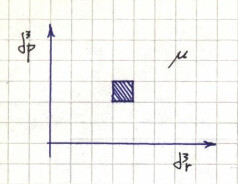
\includegraphics[scale=0.5]{images/1606329227.jpg}

Con normalización
\[
	N = \int \int f(r,p,t) d^3r d^3p
\]
donde se integra en el espacio de fases.
El gas ideal es la aproximación más baja; el $\sigma = 0$ porque no colisiona.
Consideremos un flujo libre
\[
	(r,p) \to ( r + v \delta t, p + F \delta t )
\]
En ausencia de colisiones, $f$ se consderva. Pero si hay colisiones tiene que variar

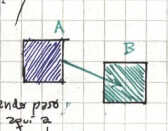
\includegraphics[scale=0.5]{images/1606329231.jpg}
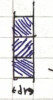
\includegraphics[scale=0.5]{images/1606329234.jpg}


En cada celda pueden convivir diferencias de momentos muy grnades entre partículas.
En el primer pic cuando paso dde aquí a aquçi si alguna partícula chocca, se modifica el $p$ de modo
que no llega a B. Posiciones cercanas y momentos (?) diferentes darán colisiones. 
En el segundo pic, estas colisionan: mismo espacio de configuración pero momento desigual

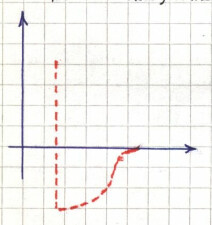
\includegraphics[scale=0.5]{images/1606329237.jpg}
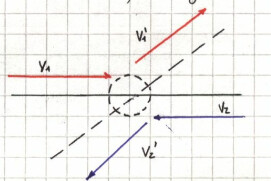
\includegraphics[scale=0.5]{images/1606329239.jpg}

Tenemos colisiones directas (asociadas a las que despueblan la celda) y colisiones inversas (asociadas
a las que pueblan la celda). La pérdida o ganancia se refiere a un salto en $\vb{p}$.
Finalmente, se tiene la ecuación de Boltzmann
\[
	\dpare{f}{t}{\text{coll}} = \int \int ( f' f'_1 - f f_1) V \sigma(V) d^2v_1 d\Omega.
\]

{\bf suelto}

El equilibrio corresponde a 
\[
	f_0(p_1) f_1(p_2) = f_0(p_1') f_1(p_2')
\]
que proviene de pedir $df/dt = 0$.
Considero, antes y después de la colisión, que estoy fuera del rango de interacción.
La distribución de Maxwell-Boltzmann (solución de equilibrio de la ecuación de Boltzmann).

\subsection{Teoría cinética}

La ecuación de transporte de Boltzmann
\[
	\left( \dpar{}{t} + \frac{\vbp}{m} \nabla_x + \vb{F}\Nabla_p \right) f(\vbx,\vbp,t) =
	\dpare{f}{t}{\text{coll}} 
\]
que vale para una situación estacionaria, donde no hay fuerzas externas $f(\vbx,\vbp,t) \to f(\vbp) $ 
(que satisface el miembro derecho nulo de la anterior) y es homogéneo (¿?).
Esta es la ecuación para la función de distribución.
Esto conduce a
\[
	f_0(\vbp) = \frac{ n }{( 2 \pi m k T )^{3/2}} \euler^{- (\vbp - \vbp_0)^2 / (2mkT)},
\]
que es la distribución de Maxwell-Boltzmann y en función de la velocidad,
\[
	f_0(\vbv) = n \Frac{ m }{2 \pi k T }^{3/2} \euler^{- m (\vbv - \vbv_0)^2 / (2kT)},
\]

Pero los ejercicios en general tienden campos externos. Los resuelvo con una perturbación
\[
	f = f_0 + f_1
\]
donde $f_0$ es MB y la otra es algo. Se requiere entonces la función de distribución de la perturbación,
que se hará considerando que $f_1 \ll f_0$
\[
	\left( \dpar{}{t} + \frac{\vbp}{m} \nabla_x + \vb{F}\Nabla_p \right) (f_0+f_1) =
	\dpare{f}{t}{\text{coll}} \approx -\frac{f_1}{\tau}
\]
donde $\tau$ es un tiempo característico medio entre colisiones.
Además se usará la hipótesis de equilibrio local la aforma de la distribución es siempre la de Boltzmann
en todo punto pero cambiand de punto a apunto $n, T, \vm{\vbv}$ que son funciones de $\vbx$ y, eventualmente,
del tiempo.

Sin embargo, pensaremos que estas variaciones serán suaves y relacionadas en el tiempo con el $\tau$.
Las variaciones de $f_1$ serán muy pequeñas. A igual orden, podemos pensar que
\[
	\left( \dpar{}{t} + \frac{\vbp}{m} \nabla_x + \vb{F}\Nabla_p \right) f_0 \approx -\frac{f_1}{\tau}
\]
con 
\[
	\dpare{f}{t}{\text{coll}}  = 0
\]

\begin{ejemplo}{\bf Problema 5}

Tenemos la situación ilustrada en la figura debajo

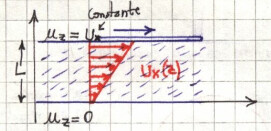
\includegraphics[scale=0.5]{images/1606329328.jpg}

donde se tiene
\[
	u_x(z) = \frac{u_x}{L} z
\]
con $\vm{v_x} = u_x(z)$.

A un plano dado la parte inferior retrasa a la parte de arriba. Para mantener el perfil hay que meter
energía que se va en el rozamiento.
La fuerza experimental por el fluido superior en la unidad de tiempo
\[
	f_\text{fricción} = - \mu \dpar{u_x}{z}
\]
donde $\mu$ es la constante de viscosidad.

Hay intercambio de partículas es a ritmo constante por el supuesto flujo laminar

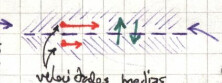
\includegraphics[scale=0.5]{images/1606329331.jpg}

lo que no está balanceado es el flujo de momentos; eso es lo que genera el frenado.
La cantidad transportada es $ m (v_x - u_x)$ donde la primera es la velocidad de las partículas, y
el flujo efectivo será $n (v_z - u_z )$
\[
	f_\text{fricción} = m n ( v_x - u_x ) (v_z - u_z )
\]
donde $u_x, u_z$ son velocidades medias. Entonces
\[
	P_{zx} = m n \vm{ (v_x - u_x) v_z }
\]
donde $\vm{u_z}=0$ pues no hay flujo neto en la dirección $\hat{z}$. Es el flujo en $\hat{z}$ de vector
$\vbp$ en $\hat{x}$.

\[
	f = f_0 ( v_x - u_x(z), v_y,m v_z ) + f_1
\]
y pensando en el estacionario y sin fuerzas externas
\[
	\frac{\vbp}{m} \nabla_x f = \dpare{f}{t}{\text{coll}}
\]
\[
	v_z \dpar{f_0}{z} = - \frac{f_1}{\tau} = - v_z \dpar{f_0}{U_x}(U_x,U_y,U_z) \dpar{U_x}{z}
\]
con $U_x = v_x - u_x(z)$ y $u_j=v_j$ para $j=y,z$.
De manera que ahora es
\[
	f = f_0 + \tau v_z \dpar{f_0}{U_x} \dpar{U_x}{z}
\]
y debo estimar
\[
	P_{zx} = m n \vm{U_zU_z}_{f_0+f_1}
\]
pero $\vm{U_xU_z}_{f_0} = 0$ por la simetría de la distribución de MB.
\[
	P_{zx} = n m \tau \int d^3 U \: U^2_z U_x \dpar{f_0}{U_x} \dpar{U_x}{z} =
	- n \tau m^2 \beta \dpar{U_x}{z} \vm{ U_z^2 U^2_x}_{f_0}
\]
\[
	\vm{ v_z^2 }_{f_0} = \frac{ k T }{m} = \frac{1}{\beta m} \qquad 
	P_{zx} = - n \tau m^2 \beta \dpar{U_x}{z} \frac{1}{\beta^2 m^2 }
\]
\[
	P_{zx} = - \frac{n \tau}{\beta} \dpar{U_x}{z}
\]
donde el factor que está pegado a la derivada es la viscosidad $\eta$ de manera que
\[
	\eta = n \tau k T.
\]

La otra parte pide calcular una conductividad

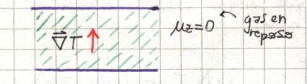
\includegraphics[scale=0.5]{images/1606329338.jpg}

y quiero ver el flujo de calor (flujo de energía cinética)
\[
	\bar{Q} = n \frac{m}{2} \vm{ \vbv v^2 }
\]
forzamos la existencia de un gradiente de temperatura y llegamos a la misma ecuación
\[
	\left( \dpar{}{t} + \frac{\vbp}{m} \nabla_x + \vb{F}\Nabla_p \right) f_0 = - \frac{f_1}{\tau}
\]
y con 
\[
	f_1 = - \tau v_x \dpar{f_0}{z}
\]
es
\[
	f_0 = n(z)\Frac{ m \beta(z) }{ 2 \pi }^{3/2} \euler^{ - \beta(z)/2 m ( \vbv - \vm{\vbv})^2}
\]
donde la velocidad media es nula por estar en reposo.

Usando regla de la cadena,
\[
	f_1 = - \frac{\tau}{n} \dtot{n}{z} f_0 v_z - \tau v_z \dpar{f_0}{\beta} \dpar{\beta}{z}
\]
y queremos ver si las derivadas $\partial n/\partial z$ y $\partial \beta / \partial z$ están relacionadas.
Como estoy en equilibrio y no hay movimiento neto,
\[
	\vm{v_z}_{f_0+f_1} = 0 \quad \to \quad \vm{v_z}_{f_1} = 0
\]
y $\int f_1 v_z d^3v = 0$ donde se puede amasar para llegar a
\[
	\dtot{n}{z} = - k \beta h \dtot{T}{z},
\]
luego
\[
	f_1 = \frac{\tau}{T} \dtot{T}{z} \left[ f_0 + \frac{1}{kT}\dpar{f_0}{\beta} \right] v_z
\] 
y
\[
	Q_z = \frac{1}{2} n m ( \vm{ v^2_x v_z } + \vm{ v^2_y v_z } + \vm{ v_z^3 } )
\]
\[
	Q_z = \frac{\tau}{T} \dtot{T}{z} \frac{ n m }{2} \left( 1 + \frac{1}{kT}\dpar{}{\beta} \right)
	\int d^3v ( v_x^2 v_z^2 + v_y^2 v_z^2 + v_z^4 ) f_0
\]
donde la integral debería dar $ 5 /m^2 (kT)^2$, entonces
\[
	Q_z = - \frac{5}{2}  \tau n k^2 T  \dtot{T}{z} \equiv \kappa \dtot{T}{z}
\]
y podemos considerar el cociente
\[
	\frac{\kappa}{\eta} = \frac{ 5/2 \tau n T k^2 }{ n \tau \kappa T } = \frac{5}{2}k
\]

La aproximación consiste en poner $f=f_0 +f_1$ y 
\[
	\dpare{f}{t}{\text{col}} \sim - \frac{f_1}{\tau}
\]
que es la aproximación de tiempo de relajación.
 
\end{ejemplo}

\begin{ejemplo}{\bf Problema 6}

Estimar densidad de corriente. Los electrones no sienten el campo de los iones.
Planteamos la ecuación 
\[
	\dpar{f}{t} + \vbv \nabla_x f_0 + \frac{\vb{F}}{m}\nabla_p f_0 = -\frac{f_1}{\tau}
\]
con $\vb{E}=E\zver$ y $\vb{F}=-eE\zver$ de manera que $f_1 = - e E 2 \beta v_z f_0$
y el flujo que interesará calcular será $J_z = - n e \vm{ v_z } $.

\notamargen{Puede ser que no haga falta ir a $\tau$ si puedo tener algo que rompe 
la simetría de traslación; entonces meto $f_0(\vbx,\vbp)$.}

\end{ejemplo}





\subsection{Ensamble gibbsiano}

Dada una condición macroscópica ($U,V,N$) puedo construirme todos los estados compatibles con esa condición.
Tendré una densidad de estos estados en $\Gamma$.
Paredes reflectantes al 100\% implican conservación de la energía

Desde $\Gamma \to \mu$ (espacio de celdas discreto; un grano grueso)
\[
	\sum_i n_i = N
\]
de manera que un punto en $\Gamma$ va a una $f$ en $\mu$, y $f$ en $\mu$ va a un volumen en $\Gamma$
(muchos puntos en $\Gamma$). De manera que la $f$ con mayor volumen será la más probable.


Considero partículas distinguibles, y así se llega a
\[
	f_i \propto C \euler^{ - \beta \varepsilon_i }
\]

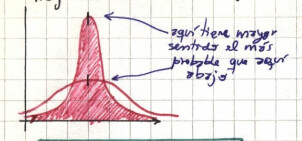
\includegraphics[scale=0.5]{images/1606329273.jpg}

\notamargen{Lo que cuenta es el ancho de la campana (figura).}


Queremos encontrar el extremo de $\Omega(n)$. Con $N\to\infty$ en Boltzmann la distribución MB es la dominante
(independientemente del hamiltoniano). La $\sigma$ es nula.

\section{Teorema H}

Si $H$ es constante en el tiempo entonces $f$ será constante. Se considera $H \equiv \int d^3v f \log (f)$
\[
	\dtot{H}{t} \leq 0,
\]
y esto define una flecha del tiempo.
Entonces como $H$ es siempre no positiva, $H$ será acotada y entonces se llega al mínimo y se queda ahí.
Pero esto es incompatible con el teorema de Poincaré, por ejemplo. Luego se vio que en realidad $H$ fluctúa.

Las ecuaciones de la mecánica (sistemas aislados no disipativos) son invertibles temporalmente.
El teorema H de Boltzmann parece ser violado si miramos en una escala de tiempo que no nos muestra
la \textit{picture} completa.

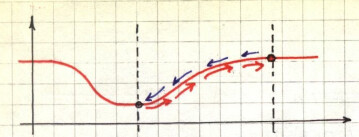
\includegraphics[scale=0.5]{images/1606329246.jpg}

Por el camino azul parece violar el tema de minimizar $H$ en el avance temporal.

\section{Ensamble}

Un ensamble es un conjunto de puntos en el espacio $\Gamma$.
Consideramos una condición de un sistema con $U,V,N$ entonces tendrá ciertos valores de $p,q$ (que
evolucionan en el tiempo como el hamiltoniano predice). Dará una cierta $\rho(p,t)$.
Tenemos el teorema de Liouville
\[
	\dpar{\rho}{t} + \sum_i \left[ \dpar{\rho}{p_i} \dot{p}_i + 
	\dpar{\rho}{q_i} \dot{q}_i \right] = 0
\]
y entonces la condición
\[
	\dtot{\rho}{t} = 0,
\]
nos habla de un {\it fluido} incompresible.
Entonces, la densidad de puntos en el espacio $\Gamma$ no varía. Los volúmenes se conservan; es una
consecuencia de los volúmenes aislados. No se crean ni aniquilan puntos.

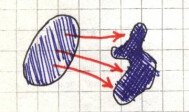
\includegraphics[scale=0.5]{images/1606329250.jpg}

Según ilustra la picture se conserva el número de puntos en la transformación.

La jerarquía BBGKY son unas ecuaciones acopladas que dan la evolución de las funciones de distribución
en función de las otras.

El ensmable microcanónico corresponde a $U,V,N$ fijos con paredes perfectamente reflectantes.
La condición sobre $U$ es que hay un mapeo de $\Gamma$ a $\mu$ que define un número de ocupación,
pero en esa transformación se pierde información microscópica; se pierde datos porque de un punto en
$\Gamma$ paso a unas celdas en $ \mu $.

Quiero exrtremar el número de ocupación y, con aproximación de Stirling mediante, se llega a
\[
	\tilde{f} = C \euler^{-\beta \epsilon},
\]
una distribución normal para la distribución más probable. Una distribución \textit{chancha} no nos da mucha
información mientras que una \textit{picuda}, en cambio, sí.

La cantidad
\[
	\rho(\{ \vec{q}_i, \vec{p}_i\},t) d^{3N}qd^{3N}p
\]
es el número de microestados en el elemento $d^{3N}qd^{3N}p$ al tiempo $t$ centrado en $q,p$.
Si los microestados son equiprobables $\rho \equiv cte.$. El conjunto $\{ \vec{q}_i, \vec{p}_i\}$ son
$6N$ coordenadas.
\[
	\Omega = \int p d^{3N}qd^{3N}p
\]
\notamargen{La integral $\Omega$ es imposible porque es difícil determinar el volumen de integración.}

XXX Dibujos XXXX

el volumen en  $\mathbb{\Gamma}$ es proporcional al número de microestados compatibles con $E,N$,
el volumen $ \mathbb{\Gamma}$ del macroestado es $\Omega\{ n_i \}$

$n_i = f_i d^3q d^3p$ es el número de partículas en una celda $i$ (con su $\vec{p}$ en $\vec{p} + d\vec{p}$
y con su $\vec{q}$ en $\vec{q} + d\vec{q}$ )

Un microestados determina una distribución $f$ que da un conjunto $\{ n_i \}$. Pero una $f$ determina muchos
microestados porque la función de distribución no distingue entre partículas (importan los números de 
ocupación); entonces una $f$ determina un volumen en $\mathbb{\Gamma}$.
\notamargen{Cada microestado tiene su $f$.}

Suponemos que todos los microestados en $\mathbb{\Gamma}$ son igualmente probables.
La $f$ que determina el mayor volumen en  $\mathbb{\Gamma}$ es la más probable. Suponemos que en el 
equilibrio el sistema toma la $f$ más probable.
Si $f_i$ es el valor de $f$ en cada celda $i$
\[
	f_i = \frac{n_i}{d^3p d^3q} \quad \text{promediada en el ensamble} \quad \bar{f}_i =  \frac{<n_i>}{d^3p d^3q}
	\quad \text{en el equilibrio}
\]
\notamargen{$f_i$ es la distribución para un miembro en el ensamble.}

Esta $\bar{f}_i$ es la de equilibrio, pero la cuenta no es fácil. Asumiremos que la $f$ de equilibrio es la más
probable (la de mayor volumen en  $\mathbb{\Gamma}$); entonces maximizaremos dicho volumen para hallarla.

Un microestado determina una $f$; diferentes microestados pueden determinar otras $f$ pero muchos coincidirán en
una misma $f$.

La $f$ en el equilibrio es la que tiene mayor cantidad de microestados (la más probable) pero 
\[
	\bar{f}_i =  \frac{<n_i>}{d^3p d^3q}
\]
es el promedio en el ensamble y no será exactamente igual a la $f_i$ del mayor volumen, salvo que el volumen de $f$
sea mucho mayor al ocupado por $f',f''$, etc.

Dado el volumen $\Omega \{ n_i\}$ extremaremos el mismo sujeto a las condiciones
\[
	E = \sum_i^K n_i e_i \qquad \qquad N = \sum_i^K n_i
\]
y llegamos a la $f$ de equilibrio que es $f_{MB}$.
\notamargen{Necesito $\Omega = \Omega \{ n_i\}$ para obtener el $\{ \tilde{n}_i\}$.}

El volumen $\Omega$ se escribe en función de los números de ocupación
\[
	\Omega \left( \{ n_i \} \right) = 
	\frac{N!}{\prod_i^K n_i!} \prod_i^K g_i^{n_i} \qquad 
	(i=1,2,...,K \quad \text{identifica celdas en}\;\mu )
\]
\[
	\Omega \left( \{ n_i \} \right) = N! \prod_i^K \frac{g_i^{n_i}}{n_i!}
\]
donde $g_i$ son los subniveles en que podríamos dividir la celda $K$; es por matemática conveniencia y para abarcar 
más casos (luego será $g_i=1 \forall i$).

El conjunto $\{ \tilde{n}_i\}$ que extrema $\Omega \left( \{ n_i \} \right)$ es el más probable y consideraremos
\[
	\{ \tilde{n}_i\} = < n_i >
\]
Estaremos pensando que cuando $N \to \infty$ la mayor parte de los microestados van a una distribución $f_{MB}$


% =================================================================================================
\section{Microcanónico}
% =================================================================================================

\subsection{Solución de equilibrio}

La solución de equilibrio satisfacía
\[
	f(p_1) f(p_2) = f(p_1') f(p_2')
\]
\[
	\log f(p_1) + \log f(p_2) = \log f(p_1') + \log f(p_2')
\]
que luce como una ley de conservación y admite como solución
\[
	\log f(p) = A m + \vb{B}\cdot \vb{p} + C|\vb{p}|^2 
	\qquad (A,\vb{B},C \text{ctes. adimensionales})
\]
que lista los {\it invariantes colisionales}. Completando cuadrados
\[
	f \propto C_1 \euler^{-C_2(\vb{p} - \vb{p}_0)^2}
\]

La expresión completa se ajusta con 
\[
	n = \int f(\vb{p},t) d^3p
\]
donde el $\vb{p}$ de una partícula es
\[
	<\vb{p}> = \frac{\int f(\vb{p}) \vb{p} \; d^3p d^3q}{\int f(\vb{p}) \; d^3p d^3q } = 
	\frac{1}{n} \int f(\vb{p}) \; \vb{p} \; d^3p
\]
\notamargen{El cociente es $\vb{P}/N$.}
y la energía por partícula
\[
	<e> = \frac{\int f(\vb{p}) \; \vb{p}^2/ (2m) \; d^3p d^3q}{\int f(\vb{p}) d^3p d^3q } = 
	\frac{1}{n} \int f(\vb{p}) \frac{ \vb{p}^2 }{ 2m } \; d^3p
\]

Finalmente se llega a 
\[
	f(\vb{p}) = \frac{n}{(2\pi m k T)^{3/2}} \euler^{- \frac{( \vb{p} - \vb{p}_0 )^2}{2mkT} }
\]

que es la función de distribución de momentos de Maxwell-Boltzmann.
\notamargen{Solución de equilibrio de la ecuación de transporte}

\[
	\text{(presión ideal)} \qquad p = \frac{2}{3} \frac{U}{V} = \frac{2}{3} n \epsilon =
	\frac{2}{3} n \frac{3}{2} k T = nkT 
\]

\subsection{Método de la distribución más probable}

Con este método también llegamos a $f_{MB}$ pero extremandolo el volumen $\Omega(\{ n_i \})$ que ocupa en el espacio
$\mathbb{\Gamma}$ sujeto a los vínculos $E = \sum_i n_i e_i$ y $N = \sum_i n_i $.

Luego podemos estimar qué tan probable es la distribución de MB (la más probable) considerando
(ASUMIMOS)
\[
	\text{los \# de ocupación de MB} \quad \tilde{n}_i \cong <n_i> \quad \text{el promedio en el ensamble}
\]
pero esto sólo valdrá si las desviaciones son pequeñas; es decir si $f_{MB}$ es muy muy probable.

Calculamos la desviación cuadrática (varianza) se tiene 
\[
	<n_i^2> - <n_i>^2 = g_i \dpar{<n_i>}{g_i}
\]
donde se usó que 
\[
	<n_i> = \frac{\sum_{\{ n_j\}} n_i \Omega\{ n_j\} }{\sum_{\{ n_j\}} \Omega\{ n_j\}}
\]

Suponiendo que $ <n_i> \approx \tilde{n}_i$ entonces $ <n_i>  \propto f_{MB}$ con lo cual se tiene también 
\[
	<n_i^2> - <n_i>^2 \cong \tilde{n}_i
\]
\notamargen{como $ g_i \dpar{\tilde{n}_i}{g_i} = \tilde{n}_i $}
y las fluctuaciones relativas
\[
	\sqrt{<\left( \frac{m_i}{N}\right)^2 > - <\left( \frac{m_i}{N}\right) >^2 } \cong 
	\sqrt{ \frac{ \tilde{n}_i/N }{N} }\to_{N\to\infty} 0
\]

En el límite termodinámico MB es totalmente dominante.

\subsection{Hipótesis ergódica}

La trayectoria individual de casi cualquier punto en el $\Omega$ pasa, con el tiempo, a través de todos los
puntos permitidos del espacio $\mathbb{\Gamma}$. Si esperamos lo suficiente, todos los microestados posibles
son visitados.

Considerando un $H$ independiente del tiempo. Coinciden los promedios:
\begin{itemize}
 \item Seguir cada trayectoria, resolviendo las ecuaciones de movimiento hasta tiempo infinito.
 \item Calcular valor medio en el espacio $\Gamma$
\end{itemize}


\subsection{Observaciones sobre el microcanónico}

\[
	\Gamma(E) = \int_{E < \Ham < E + \Delta E} \rho d^{3n}p d^{3n}q \qquad 
	\Sigma(E) = \int_{\Ham < E} \rho d^{3n}p d^{3n}q
\]
entonces 
\[
	\Gamma(E) = \Sigma( E + \Delta E ) - \Sigma( E ) \cong \dpar{\Sigma( E )}{E}\Delta E  
	\qquad \text{si}\; \Delta E \ll E
\]
$\Delta E$ es el {\it paso} entre medidas de energía 
\[
	\Gamma(E) = \Gamma_1(E_1) \Gamma_2(E_2) \qquad \text{(1 y 2 son subsistemas)}
\]
\[
	E = E_1 + E_2 \Rightarrow \Gamma(E) = \sum_i^{E/\Delta E} \Gamma_1(E_i)\Gamma_2(E-E_i)
\]
siendo $E/\Delta E$ el número de términos tales que se cumple $ E = E_1 + E_2 $.
Si se da $ N_1 \to \infty $ y $ N_2 \to \infty $ será
\[
	\log \Gamma_1 \propto N_1 \quad \log \Gamma_2 \propto N_2 \quad E \propto N_1 + N_2
\]
luego $\log(E/\Delta E)$ es despreciable pues $\Delta E$ es constante y entonces
\notamargen{$\log(E/\Delta E) \propto \log(N)$ pues $E\propto N$ y $\Delta E$ cte.}
\[
	S(E,V) = S(\tilde{E}_1,V_1) + S(\tilde{E}_2,V_2) + \mathcal{O}(\log[N])
\]
con lo cual la mayoría de los microestados tienen los valores $\tilde{E}_1$ y $\tilde{E}_2$ de energía.

Asimismo
\[
	\delta( \Gamma_1(\bar{E}_1)  \Gamma_2(\bar{E}_2) ) = 0 \qquad \delta( \bar{E}_1 + \bar{E}_2 ) = 0
\]
\[
	\delta\Gamma_1 \Gamma_2 + \Gamma_1 \delta \Gamma_2 = 0 \quad \delta( \bar{E}_1 ) = -\delta ( \bar{E}_2 )
\]
\[
	\frac{\delta\Gamma_1}{\bar{E}_1}\Gamma_2 = \Gamma_1\frac{\delta\Gamma_2}{\bar{E}_2} \Rightarrow 
	\frac{1}{\Gamma_1} \dpar{\Gamma_1}{\bar{E}_1} = \frac{1}{\Gamma_2} \dpar{\Gamma_2}{\bar{E}_2} 
\]
\[
	\dpar{}{\bar{E}_1}\left( k\log \Gamma_1(\bar{E}_1) \right) = 
	\dpar{}{\bar{E}_2}\left( k\log \Gamma_1(\bar{E}_2) \right)
\]
\[
	\left. \dpar{}{{E}_1}S(E_1)\right|_{\bar{E}_1} = \left. \dpar{}{{E}_2}S(E_2)\right|_{\bar{E}_2}
	\equiv \frac{1}{T} \qquad \text{en equilibrio} \; T_1 = T_2
\]

La $T$ es el parámetro que gobierna el equilibrio entre partes del sistema.

La idea es que dado un sistema de $E = E_1 + E_2$, sistema compuesto de dos subsistemas, hay muchos valores
1,2 tales que $E = E_1 + E_2$ pero hay una combinación que maximiza $\Gamma(E)$ y es
\[
	\Gamma_{Max}(E) = \Gamma_1(\bar{E}_1)  \Gamma_2(\bar{E}_2) 
\]
\notamargen{El sistema es $E,N,V$ y yo lo pienso compuesto de dos partes $E_1,N_1,V_1$ y $E_2,N_2,V_2$.}

Luego, con $N_1, N_2 \to \infty$ se da que la mayoría de los sistemas tendrán $E_1=\bar{E}_1$ y $E_2=\bar{E}_2$.
Esa configuración, por supuesto, maximiza la entropía $S=k\log(\Gamma)$.

El hecho de que $\Delta S> 0$ para un sistema aislado lo vemos considerando que tal sistema sólo puede variar
$V$ (creciendo, como en la expansión libre de un gas), luego $V_F > V_I$ y entonces
\[
	\Sigma(E) = \int_{\Ham < E} \rho d^{3N}p d^{3N}q \underbrace{\longrightarrow}_{\text{Si aumento el volumen}}
	\Sigma(E)' = \int_{\Ham < E} \rho d^{3N}p d^{3N}q
\]
\notamargen{Será un número mayor porque el dominio de integración en $q$ es mayor.}
\[
	\Sigma(E)' > \Sigma(E) \qquad \Rightarrow \qquad \Delta S > 0
\]

Equipartición implica 
\[
	\left< x_i \dpar{\Ham}{x_j} \right> = \delta_{ij} k T
\]
y entonces
\[
	\left< p_i \dpar{\Ham}{p_i} \right> = \left< p_i \dot{q}_i \right> = kT 
\]
y
\[
	\left< q_i \dpar{\Ham}{q_i} \right> = \left< q_i \dot{p}_i \right> = kT 
\]
\[
	\left< \sum_i^{3N} q_i \dpar{\Ham}{q_i} \right> =  \sum_i^{3N} \left< q_i \dpar{\Ham}{q_i} \right> =
	\sum_i^{3N} k T = 3 N k T
\]
entonces llegamos al virial,
\[
	\sum_i^{3N} \left< q_i \dot{p}_i \right> = 3 N k T.
\]

Considerando un hamiltoniano armónico,
\[
	\left< \Ham \right> = E \qquad \text{con} \quad \Ham = \sum_i^{3N} a_i p_i^2 + b_i q_i^2
\]
\[
	p_k \dpar{\Ham}{p_k} = 2 a_k p_k^2 \qquad q_k \dpar{\Ham}{q_k} = 2 b_k q_k^2
\]
de modo que 
\[
	\Ham =  \sum_i^{3N} \frac{1}{2} p_k \dpar{\Ham}{p_k} + \frac{1}{2} q_k \dpar{\Ham}{q_k}
\]
\[
	\left< \Ham \right> =  \sum_i^{3N} \frac{1}{2} \left< p_k \dpar{\Ham}{p_k}\right> +
		\frac{1}{2} \left< q_k \dpar{\Ham}{q_k} \right>
\]
y si $f$ es el número de constantes $a_k,b_k$ no nulos
\[
	\left< \Ham \right> =  \frac{1}{2} f k T
\]

Si fuesen todas no nulas entonces
\[
	\left< \Ham \right>  = 3 N k T.
\]

{\bf Suelto para reprocesar}

Ensambles calcula valores medios sumando sobre todos los
\[
	N \to  \infty, \quad V \to \infty \qquad \frac V N = v
\]

Para un sistema aislado, equiprobabilidad a priori, $\rho=$ cte es solución si ajusta a $P,V,T$
\[
	S(U,V) = k \log T(U)
\]
donde supondremos que $U$ es aditiva. Como $E=E_1 + E_2$ el volumen en el espacio de fases
\[
	\Gamma(U) = \sum_{i j} \Gamma_1(E_1)\Gamma_2(E - E_1)
\]
de dos sistemas separados y luego reunidos.
En el equilibrio $T_1=T_2$

Además el crecimiento de la entropía en el sistema aislado. Expansión libre: $q$ crece entonces 
$\Gamma$ crece.

Pero por Liouville $V_\Gamma$ no varía de modo que la evolución en el espacio de fases hará que
ciertos estados sean inalcanzables ({\it mixing}).

Tenemos la paradoja de Gibbs porque hemos estado considerando partículas indistinguibles; entonces
al considerar la indistinguibilidad debemos sumar menos (es decir que hay que dividir por un
factor). Sin embargo, la indistinguibilidad es un concepto no clásico.
Es $ \Delta S > 0 $ con distinguibles y $ \Delta S = 0 $ si son distinguibles.
Esta corrección por distinguibilidad no tiene fundamento clásico.

Boltzmaniones: partículas en las cuales uso todas las herramientas clásicas y al final solo
corregimos con un factor $1/N!$ por indistinguibilidad.


\subsection{Fenómenos de transporte}

Un gas clásico verifica
\[
	\frac{\hbar}{\sqrt{2 m k T}} \Frac{N}{V}^{1/3} \sim 0.0004 \ll 1
\]
donde el primer factor es la longitud de onda de DeBroglie de modo que es un ratio 
del tipo $\lambda / \ell$ porque el segundo término es la inversa del volumen por
partícula elevado a la un tercio.

Entonces
\[
	f(\vb{x}, \vb{p}, t ) d^3x d^3p 
\]
es el número de partículas que se hallan entre $\vb{x}, \vb{x} + d \vb{x}$ y con 
$(\vb{p}, \vb{p} + d \vb{p} )$ en un tiempo $t$.

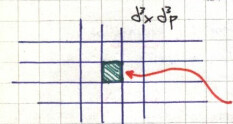
\includegraphics[scale=0.5]{images/1606329279.jpg}


Hay un número grande de partículas en cada celda. Es un diferencial no matemático (un {\it cachito})
puesto que no tenderá a cero.

\begin{ejemplo}{\bf Problema 3}

Se consider un gas clásico de $N$ partículas
\[
	\int \int f(\vb{x}, \vb{p}, t ) d^3x d^3p = N \qquad \qquad 
	\int f(\vb{x}, \vb{p},t) d^3p = n
\]
y asociamos a una partícula una $\alpha(\vb{x}, \vb{v}, t)$ donde ($\alpha$) serán cantidades extensivas.

El flujo de $\alpha$ se ilustra así
 
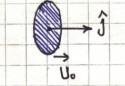
\includegraphics[scale=0.5]{images/1606329282.jpg}

de modo que
\[
	\vm{\alpha}(\vb{x},t) = \frac{\int \alpha(\vb{x},\vb{p}, t) f(\vb{x},\vb{p},t) d^3p}
	{\int f(\vb{x}, \vb{p},t) d^3p} =
	\frac{1}{n} \int \alpha(\vb{x},\vb{p}, t) f(\vb{x},\vb{p},t) d^3p
\]
Y entonces,
\[
	\hat{j} \cdot \int d^v \alpha(\vb{v}-\vb{u}_0) f(\vb{x},\vb{p},t) =
	\hat{j} \cdot \vm{ \vb{v}-\vb{u}_0 \cdot \alpha } n(\vbx,t),
\]
de manea que el flujo de $\alpha$ es todo lo que multiplica a la dirección $\hat{j}$.

Recordemos la consideración usual microscópica para el flujo ilustrada a continuación:

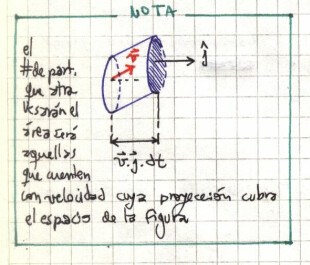
\includegraphics[scale=0.5]{images/1606329287.jpg}

{\bf Densidad de corriente}

Será la carga por unidad de tiempo en una superficie
\[
	\phi_e = n(\vb{x},t) \cdot \vm{\hat{j}\cdot \vb{v}_q}
\]
o bien 
\[
	\vec{\phi}_e =  n(\vb{x},t) \vm{\vb{v}_q}
\]
luego será $\phi_e = n q \vm{ \hat{j} \cdot \vb{v} }$

{\bf Flujo térmico (calor)}
\[
	Q = n(\vb{x},t) \vm{ 1/2 m v^2 \vb{v} }
\]
donde $ \alpha = 1/2 m v^2 $ es la densidad de energía cinética (asociada a temperatura)

{\bf $P_{ij}$ flujo de momento}

\[
	\alpha(\vbx, \vb{v}, t) = m ( \vm{v}_i - \vm{v_i} )
\]
\[
	P_{ij} = m \vm{  (\vm{v}_i - \vm{v_i}) v_j } n
\]
y se ve que el flujo de momento es claramente un tensor.

Sea la distribución $f(\vbx, \vbv, t )$ y entonces quiero llegar al equilibrio y ver que ya no
depende del tiempo. La ecuación que define la evolución temporal de $f$ es la ecuación de
Boltzmann.

Si no hay colisiones debe valer
\[
	\vbp_i \to \vbp_i + \vb{F} \delta t \qquad 
	\vbx_i \to \vbx_i + \vbv \delta t
\]
pero el número de partículas se mantiene constante
\[
	f(\vbx,\vbp, t) d^3x d^3p = f(\vbx',\vbp', t') d^3x' d^3p'
\]
y con sistema hamiltoniano es $ d^3x d^3p = d^3x' d^3p'$.
Lo que estamos diciendo es que por colisiones hay partículas que chocan y va a parar a otro $\delta V$
y hay otras que chocan y por ello vienen a parar a este $\delta V$; hay ganancia y pérdida.
Entonces,
\[
	f(\vbx,\vbp, t) = f(\vbx + \vbv \delta t,\vbp + \vb{F} \delta t, t + \delta t)
\]

Si $\delta t=0$ se tiene $df/dt=0$ de lo cual deducimos
\[
	\left( \dpar{}{t} + \frac{\vbp}{m} \nabla_x + \vb{F}\Nabla_p \right) f(\vbx,\vbp,t) = 
	\begin{cases}
	 0 \quad \text{ No hay colisiones}\\
	 \dpar{f}{t} \quad \text{ Hay colisiones}\\
	\end{cases}
\]
\[
	\dpar{f}{t} dt = (G-P) dt
\]
donde $P \delta t d^3x d^3p$ es el número de colisiones en $(t,t+\delta t)$ en las cuales una de las
partículas inicialmente estaba en las cercanías de $(\vbx,\vbp)$ y luego se va a otro lado.
Asimismo, $G \delta t d^3x d^3p$ es el número de colisiones en $(t,t+\delta t)$ en las cuales una de las
partículas termina en $(\vbx,\vbp)$ habiéndose hallado en otro lugar antes.
Consideramos un gas diluído; colisiones binarias (se desprecian eventos de tres partículas).

\[
	P \delta t d^3x d^3p_1 = \delta t d^3x d^3p_1 \int d^3 p_2 dP_{12\to 1'2'} F(\vbx,\vbp_1,\vbp_2,t)
\]
(que es una probabilidad conjunta) como las partículas chocan, entran en el mismo $\delta x$.
El término $dP$ es la matriz de transición de momentos $1,2 \to 1',2'$

\[
	G \delta t d^3x d^3p_1 = \delta t d^3x d^3p_1 \int d^3 p_2 dP_{1'2'\to 12} F(\vbx,\vbp_1',\vbp_2',t)
\]
y entonces
\[
	P = \int d^3p_2 d^3p_1' d^3p_2' \delta^4(p_i-p_f) |T_{fi}|^2 F(\vbx,\vbp_1,\vbp_2,t)
\]
donde hay deltas para la conservación de la energía y el momento.


Hay una hipótesis de caos molecular; no hay correlación entre posiciones y momento
\[
	f(\vbx,\vbp_1,\vbp_2,t) = f(\vbx,\vbp_1,t) f(\vbx,\vbp_2,t) 
\]
de suerte que
\[
	\left( \dpar{}{t} + \frac{\vbp}{m} \nabla_x + \vb{F}\Nabla_p \right) f(\vbx,\vbp,t) =
	\int d^3p_2 d^3p_1' d^3p_2' \delta^4(p_i-p_f) |T_{fi}|^2 (f_2' f_1' -  f_1 f_2)
\]

Supongamos que no hay fuerzas externas, $\vb{F}=0$ de modo que $ f(\vbx,\vbp,t)\to f(\vbp)$ en el equilibrio.
Luego, en el equilibrio
\[
	\left.\dpar{f}{t}\right|_\text{col} = 0 \qquad \longrightarrow \qquad  f_2' f_1' =  f_1 f_2
\]
aunque se puede demostrar que vale también la vuelta (es decir que es un ``sí y sólo sí'').
Cualquier distribución de equilibrio satisfará la condición anterior. Hay una forma general de 
función de equilibrio que tiene la forma
\[
	f_\text{eq}(\vbp) = C \euler^{- A(\vbp - \vbp_0)^2}
\]

Para calcular las constatnes se evalúan la presión que se ejerce sobre una pared del sistema termodinámico
usando el flujo de momento lineal


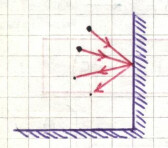
\includegraphics[scale=0.5]{images/1606329297.jpg}

Será
\[
	P = \int d^p 2 p_x v_x f_\text{eq}(\vbp)
\]
dado que la presión se relaciona con el flujo de momento.

Así llegamos a la función de Maxwell-Boltzmann
\[
	f_\text{eq}(\vbp) = \frac{ n }{( 2 \pi m k T )^{3/2}} \euler^{- (\vbp - \vbp_0)^2 / (2mkT)},
\]
que es la solución estacionaria de la ecuación de transporte de Boltzmann.
 
\end{ejemplo}

\begin{ejemplo}{\bf Problema 4}
 
\[
	\dpar{f}{t} + \frac{\vbp}{m} \dpar{f}{\vbx} + \frac{\vb{F}}{m}\dpar{f}{\vb{u}} =
	\left.\dpar{f}{t}\right|_\text{col} = 0,
\] 
en el campo gravitatorio terrestre, donde $\vb{F} = - m g z$ y entonces
\[
	\hat{z} v_x \dpar{f}{z} - g \hat{z} v_x \dpar{f}{v_z} = 0
\]
de modo que planteo 
\[
	f = \frac{ n(z) }{( 2 \pi m k T )^{3/2}} \euler^{- (\vbp - \vbp_0)^2 / (2mkT)}
\]
entonces, reemplazando, resulta en
\[
	\dtot{n(z)}{z} = - g \frac{m}{kT} n(z)
\]
y
\[
	n(z) = n_0 \euler^{-\beta m z g}.
\]
 
 
\end{ejemplo}



\subsection{Gas ideal (microcanónico)}

\[
	\Ham =  \sum_i^{N} \frac{p^2_i}{2m}
\]
\[
	\Sigma(E) = \frac{1}{h^{3N}} \int_{\Ham < E} d^3p_1 ... d^3p_N d^3q_1 ... d^3q_N = 
	\left( \frac{V}{h^{3N}} \right)^N \int_{\Ham < E} d^3p_1 ... d^3p_N
\]
donde la integral en $\{ q_i\}$ es inmediata porque no están los mismos en los límites y donde el
límite de integración $\Ham < E$ implica la condición 
\[
	p_1^2 + p_2^2 + ... + p_N^2 < ( \sqrt{2mE} )^2
\]
\notamargen{Es una especie de radio $2mE$.}
\[
	\Sigma(E) = C_{3N} \left[ \frac{V}{h^3} (2mE)^{3/2}\right]^N
\]

Luego,
\[
	S = k \log \left\{ C\left( \frac{V}{h^3}(2mE)^{3/2}\right)^N \right\}
\]
\[
	S = k \log C + N k \log \left[ \frac{V}{h^3}(2mE)^{3/2}\right]
\]
\notamargen{$ k\log C \approx -3/2 Nk \log 3N/2 $}
\[
	\left. \dpar{S}{E} \right|_{V,N} = \frac{1}{T} \qquad \Rightarrow \qquad \frac{1}{T} = Nk\frac{3}{2}\frac{1}{E}
\]
y entonces
\[
	E = \frac{3}{2} NkT \qquad \text{gas ideal}
\]
\notamargen{Vemos que la termodinámica es bastante insensible a las aproximaciones.}

\subsection{Paradoja de Gibbs}

\[
	S \propto Nk\log(V) + Nk \log (E^{3/2})
\]
Supongamos dos gases idénticos con la misma $\rho$ y $T$
\notamargen{Quitar la pared es una operación mental si los gases son idénticos (o al menos eso podemos pensar).}

\[
	\Delta S = Nk \log V + Nk \log (E^{3/2}) - N_1k \log V_1 - N_2k \log (E_1^{3/2})
	- N_1k \log V_2 - N_2k \log (E_2^{3/2})
\]
\[
	\Delta S = N_1 k \log \left( \frac{V}{V_1} \right) + N_2 k \log \left( \frac{V}{V_2} \right) +
		N_1 k \log \left( \frac{E}{E_1} \right)^{3/2} + N_2 k \log \left( \frac{E}{E_2} \right)^{3/2}
\]
\notamargen{Si los gases son distintos está correcto $\Delta S > 0$ pero si son idénticos no porque un estado
como F podría provenir de infinitas compartimentacionales las cuales darían todas difrentes $\Delta S$ y entonces
la entropía $S$ no sería función de estado.}
\[
	\Delta S > 0 \quad \text{pues: } \; \frac{V}{V_1} = 1 + \frac{V_2}{V_1} > 1, \frac{V}{V_2} > 1, 
	\frac{E}{E_1} > 1, \frac{E}{E_2} > 1
\]

Podemos hacer algo menos cuentoso tomando
\[
	S \propto Nk\log \left( V\left[ \frac{4\pi m E}{3 h^2 N} \right]^{3/2} \right)
\]
donde la $N$ viene de $k\log C_{3N}$ con $N \to \infty$. Vemos que $E/N$ mantiene el cambio en $S$ respecto de $E$
igual, puesto que 
\[
	\frac{E}{N} = \frac{E_1 + E_2}{N_1 + N_2} = \frac{E_1}{N_1} = \frac{E_2}{N_2} = \epsilon
\]
pero $V$ no balance. Luego la inclusión de $1/N!$ hará que 
\[
	S = k \log (\frac{1}{N!}\Sigma(E,N,V)) = k \log (\Sigma) - k\log N!
\]
de forma que resultará
\[
	S \propto Nk\log \left( \frac{V}{N}\left[ \frac{4\pi m E}{3 h^2 N} \right]^{3/2} \right)
\]
y esta $S$ sí está libre de paradoja de Gibbs.

% =================================================================================================
\section{Ensamble canónico}
% =================================================================================================



Consideramos un microcanónico con 
\[
	E = E_1 + E_2, \qquad N = N_1 + N_2, \qquad V = V_1 + V_2 
\]
donde $N_i, V_i$ están fijos y $E_i$ varían de acuerdo a
\[
	E = E_1 + E_2
\]

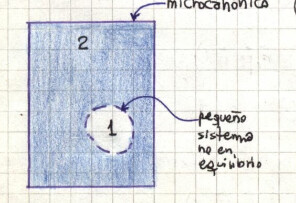
\includegraphics[scale=0.5]{images/1606329302.jpg}

La idea es que el sistema 2 es tan grande como se quiera y el sistema 1 es pequeño pero macroscópico;
entonces el primero actúa como un baño térmico. La temperatura $T$ estará fija por dicha razón, o sea
que será un problema isotérmico.


Consideramos un microcanónico 
\[
	\Gamma(E) = \Sigma_{E_1} \Gamma_1(E_1) \Gamma_2(E-E_1) \leq C \Gamma_1(\bar{E}_1) \Gamma_2(E-\bar{E}_1)
	\approx C \Gamma_2(\bar{E}_1)
\]
\[
	S(E-\bar{E}_1) \approx k \log \Gamma_2(E-\bar{E}_1)
\]
\[
	S(E) + \left.\dpar{S(E)}{E}\right|_E(-\bar{E}_1) \approx k \log \Gamma_2(E-\bar{E}_1)
\]
\[
	\euler^{\frac{S(E)}{k}} \euler^{-\frac{E_1}{kT}} \approx \Gamma_2(E-\bar{E}_1)
\]

Claramente como '1' siempre está metido dentro de '2' entre mayor sea el $\Gamma_2$ mayor también el tamaño de '1'
en $\mathbb{\Gamma}$, luego:
\[
	\# \text{de config en } \mathbb{\Gamma} \text{ del sistema '1+2'} = \# \text{de config de '1' en '2'} \times 
	\# \text{de config de '2' en} \mathbb{\Gamma}
\]
\[
	\# \text{ config '1' } = \frac{ \# \text{ config '1+2'} }{ \# \text{ config '2'} } \approx 
	\euler^{-\frac{E_1}{kT}} = C \int \euler^{-\Ham/kT} d^3p d^3q
\]
y se integra para toda energía
\[
	Q_N(V,T) = \frac{1}{h^{3N}N!}\int \euler^{-\Ham/kT} d^3p d^3q
\]
\notamargen{$1/N!$ es el factor de buen conteo.}

La función de partición es el volumen ocupado en $\mathbb{\Gamma}$.
El vínculo con la termodinámica viene de
\[
	Q_N(V,T) = \euler^{-\beta A}
\]
\[
	A = -kT\log [Q_N(V,T)]
\]
donde $A=A(T,V,N)$ es la energía libre de Helmholtz. Podemos ver que se deduce esto de 
\[
	< \Ham > = E = -\dpar{}{\beta} \log [ Q_N(V,T) ] = A + TS = A - T\left.\dpar{A}{T}\right|_{N,V}
\]
pero 
\[
	\dpar{}{\beta} = \dpar{}{T} \dpar{T}{\beta} = -k T^2 \dpar{}{T}, \qquad \text{pues } \dpar{\beta}{T} = - 
	\frac{1}{kT^2}
\]
\[
	\dpar{}{T}\left( \frac{A}{T} \right) = -\frac{A}{T^2} + \frac{1}{T}\dpar{A}{T}
\]
de modo que 
\[
	-T^2 \dpar{}{T}\left( \frac{A}{T} \right) = A - T \dpar{A}{T}
\]
\notamargen{$S=-\partial A / \partial T|_{N,V}$}
y entonces
\[
	E = -k T^2 \dpar{}{T}\log Q_N = -T^2 \dpar{}{T}\left( \frac{A}{T} \right) 
\]
de lo que se desprende
\[
	\log Q_N = -\frac{A}{kT}
\]

Podemos usar $E=A+TS$ y llegar a $Q_n=\exp(-\beta A)$ o bien $Q_N=exp(-\beta A)$ y llegar a $E=A+TS$.

\subsection{Equivalencia canónico y microcanónico}

Vemos cómo son las fluctuaciones de energía en el canónico. Desde 
\[
	U = <\Ham> = \frac{\int \euler^{-\beta\Ham} \Ham d^3p d^3q}{\int \euler^{-\beta\Ham} d^3p d^3q}
\]
\[
	\int \euler^{-\beta\Ham} U d^3p d^3q = \int \euler^{-\beta\Ham} \Ham d^3p d^3q
\]
\[
	\dpar{}{\beta}\left[ \int \euler^{-\beta\Ham} (U-\Ham) d^3p d^3q\right] = \dpar{}{\beta}\left[ 0 \right] = 0
\]
\[
	<\Ham^2> - <\Ham>^2 = kT^2C_V
\]

Las fluctuaciones van como el $C_V$, luego 
\[
	<\Ham^2/N^2> - <\Ham/N>^2 = kT^2c_V/N \qquad \text{donde } c_V = C_V/N
\]
\notamargen{$<\Ham> \propto N$ y $C_V \propto N$}
de modo que las fluctuaciones relativas van a 0 con $N\to\infty$.

Otro modo de verlo es considerando 
\[
	\frac{1}{h^{3N}N!}\int \euler^{-\beta\Ham} d^3p d^3q = \int_0^\infty dE \dpar{\Sigma(E)}{E} \euler^{-\beta E} =
	\int_0^\infty dE \euler^{-\beta E + \log (\partial \Sigma(E)/\partial E)}
\]
donde 
\[
	\dpar{\Sigma(E)}{E} dE = \frac{d^3p d^3q}{h^{3N}N!}
\]
y como $S/k = \beta TS$
\[
	Q_N = \int_0^\infty dE \euler^{-\beta E + \beta T S }
\]

Si suponemos que es $S$ máxima en $E=\bar{E}$ entonces $S_{MAX} = S(\bar{E})$ y será 
\[
	\left. \dpar{S}{E} \right|_{\bar{E}} = 0
\]
con lo cual
\[
	E + TS \cong \bar{E} + TS(\bar{E}) + \frac{1}{2}(E-\bar{E})^2 T \left. \dpar[2]{S}{E} \right|_{\bar{E}}
\]
\[
	E + TS \cong \bar{E} + TS(\bar{E}) - (E-\bar{E})^2 \frac{1}{2kTC_V}
\]
de modo que 
\[
	Q_N = \int_0^\infty dE \euler^{-\beta [\bar{E} + TS(\bar{E})] - \beta \frac{(E-\bar{E})^2}{2kTC_V}}
\]
\[
	Q_N = \euler^{-\beta [\bar{E} + TS(\bar{E})]} \int_0^\infty dE \euler^{- \beta \frac{(E-\bar{E})^2}{2kTC_V}}
\]
y vemos que la integral se va a una delta con $N\to \infty$ (pués $C_V \propto N$) en cuyo caso
\[
	Q_N = \euler^{-\beta [\bar{E} + TS(\bar{E})]} 
\]
y la mayor parte de los estados tienen energía $\bar{E}$, que es la de un sistema aislado a temperatura $T$.

La densidad de estados va entonces de acuerdo al producto de dos efectos contrarios:
\[
	g(E) = \dpar{\Sigma(E)}{E}\euler^{-\beta E}
\]

\subsection{Ejemplos sencillos}

\[
	\Ham = \sum_i^N \frac{p_i^2}{2m} + \frac{m}{2}\omega_i^2 q_i^2 \quad \qquad \text{oscilador clásico 1D}
\]
\[
	\Ham = \sum_i^N \left( n_i + \frac{1}{2} \right)\hbar\omega  \quad \qquad \text{oscilador Schrödinger 1D}
\]
\[
	\Ham = \sum_i^N  n_i \hbar\omega \quad \qquad \text{oscilador Planck 1D}
\]

\[
	U = NkT \rightarrow C_V = Nk  \qquad \text{Clásico}
\]
\[
	U \approx \frac{N\hbar\omega}{2} \quad U \approx 0 (T\ll 1) \qquad \rightarrow C_V = 0 
	\quad \text{Schrödinger-Planck}
\]
\[
	U \approx N kT \; (T \gg 1) \qquad \rightarrow C_V = Nk 
	\quad \text{Schrödinger-Planck}
\]

Los casos Schrödinger y Planck aproximan al $C_V$ clásico con $T$ altas.


\subsection{Una derivación más del canónico}

El tamaño del sistema '1' en $\mathbb{\Gamma}$ (su volumen $\Gamma_1(E_1)$) será proporcional al tamaño del sistema 
'2' en $\mathbb{\Gamma}$ (su volumen $\Gamma_2(E-E_1)$) de manera que 
\[
	\Gamma_1(E_1) \propto \Gamma_2(E-E_1)
\]
\[
	k\log \Gamma_1(E_1) \approx S(E) + \left.\dpar{S}{E}\right|_E (-E_1) = S(E) - \frac{E_1}{T} 
	\text{ (del sistema '2') }
\]
\[
	\Gamma_1(E_1) \approx \euler^{S(E)/k} \euler^{-E_1/kT} 
\]
\[
	\text{ \# conf '1' } = \text{ \# conf '2' } \times \text{ densidad del '1' en el '2' }
\]
y finalmente
\[
	Q_N (V,T) = \frac{1}{h^{3N}N!} \int d^{3N}p d^{3N}q \euler^{-\Ham(\{ p_i,q_i\})/kT}
\]

% =================================================================================================
\section{El gran canónico}
% =================================================================================================

La desventaja del microcanónico es la de tener que calcular todos los estados accesibles.
El canónino es un subconjunto del microcanónico.

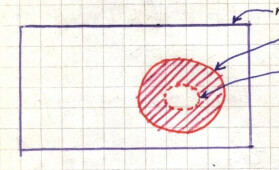
\includegraphics[scale=0.5]{images/1606329345.jpg} 
La caja es un microcanónico, el rojo es un canónico donde está fija la temperatura $T$ y el
conjuntillo más interno es una pared porosa que lo limita.

El $1/N!$ corrige la indistinguibilidad de las partículas -es el factor de buen conteo de Boltzmann-.
Se define la fugacidad $ z \equiv \euler^{ \beta \mu } $.

Para un sistema con un número de partículas determinadas puedo utilizar el GC que será más sencillo
que el MC o el C. La densidad o el número medio de partículas es algo que fijo desde fuera; el número
de partículas fluctuará y querremos calcular dicha fluctuación (que se hace en la próxima
subsección).

Todos los ensambles son equivalentes si $N \to \infty$. De lo contrario, con $N$ no infinito
tendríamos tres termodinámicas diferentes dadas por el microcanónico, el canónico y el gran canónico.
Cuando calculamos la fluctuación de energía surge una parte asociada a la variación del número de
partículas. $\partial p / \partial v = 0$ ocurre en particular en la región de coexistencia.

Se asume que el sistema satisface
\begin{itemize}
 \item Potencial tipo carozo duro + cola finita. Dado un volumen $V$ existe $N$ máximo.
 \item \[
	A(N,V) = - \frac{V}{\beta} f(\nu)
 \]
 escalea con el volumen.
 \item Como $f(\nu)$ satisface $ \partial p / \partial v \leq 0$ entonces ...
\end{itemize}

Se obtiene una función de potencial GC $\Xi$ que debe ser un polinomio en $N$ de grado 
$N_0(V) = a V$ para $V$ grande.


\[
	Q_N (V,T) =  \frac{1}{h^{3N}N!} \int d^{3N_1}p_1 d^{3N_2}p_2  \sum_{N_1=0}^N \frac{N!}{N_1! N_2!}
	\int d^{3N_1}q_1 d^{3N_2}q_2 \euler^{-\beta [\Ham_1 + \Ham_2 ]}
\]
\[
	Q_N (V,T) =  \frac{1}{h^{3N_1} h^{3N_2} } \sum_{N_1=0}^N \frac{1}{N_1! N_2!}
	\int d^{3N_1}p_1 d^{3N_1}p_1 \euler^{-\beta\Ham_1} \int d^{3N_2}q_2 d^{3N_2}q_2 \euler^{-\beta\Ham_2}
\]
\[
	Q_N (V,T) =  \sum_{N_1=0}^N \int \frac{1}{h^{3N_1}N_1!} d^{3N_1}p_1 d^{3N_1}p_1 \euler^{-\beta \Ham_1 }
	\int \frac{1}{h^{3N_2}N_2!} d^{3N_2}q_2 d^{3N_2}q_2 \euler^{-\beta \Ham_2 }
\]
\[
	1 = 
	\sum_{N_1=0}^N \frac{1}{h^{3N_1}N_1!} \int d^{3N_1}q_1 d^{3N_1}p_1 \; 
	\euler^{-\beta\Ham_1} \frac{Q_{N_2}(V_2,T)}{Q_N(V,T)} 
\]
\[
	1 = 
	\sum_{N_1=0}^N \int d^{3N_1}q_1 d^{3N_1}p_1 \; \frac{\euler^{-\beta\Ham_1}}{h^{3N_1}N_1!} 
	\frac{Q_{N_2}(V_2,T)}{Q_N(V,T)} 
\]
siendo el último factor un $ \rho(\{ p_1,q_1\},N_1)$
\[
	\frac{Q_{N_2}(V_2,T)}{Q_N(V,T)} = \euler^{-\beta A (V-V_1,N-N_1,T)}\euler^{-\beta A (V,N,T)} =
	\euler^{-\beta [ \frac{\delta A}{\delta V} \delta V + \frac{\delta A}{\delta N} \delta N ] }
\]
donde las diferencias $\delta$ se toman discretas:
\[
	\frac{\delta A}{\delta V} \delta V + \frac{\delta A}{\delta N} \delta N =
	(-p )(-V_1) + \mu (-N)_1 = pV_1 - \mu N_1
\]
\[
	A = U - TS \qquad dA = dU - TdS - SdT = -pdV + \mu dN - SdT
\]
\[
	\frac{Q_{N_2}(V_2,T)}{Q_N(V,T)} = \euler^{-\beta PV_1 + \beta \mu N_1},
\]

De forma que la densidad del sistema '1' es
\[
	\frac{1}{h^{3N_1}N_1!} \euler^{-\beta\Ham_1}  \euler^{-\beta PV_1}  \euler^{\beta \mu N},
\]
y definiendo $z \equiv \euler^{\beta\mu}$
\[
	\rho(\{p,q\},N) = \frac{z^N}{h^{3N}N!} \euler^{-\beta\Ham}  \euler^{-\beta PV} 
\]

Nótese que $ \mu, P, V, T$  son los valores fijos del sistema mayor y hemos sacado subíndices.
\[
	1 = \sum_{N=0}^\infty \int d^{3N}q d^{3N}p \frac{z^N}{h^{3N}N!} \euler^{-\beta\Ham}  \euler^{-\beta PV} 
\]
\[
	\euler^{\beta PV} = \sum_{N=0}^\infty \frac{z^N}{h^{3N}N!} \int d^{3N}q d^{3N}p \euler^{-\beta\Ham}
	= \sum_{N=0}^\infty z^N Q_N(V,T)
\]
\be
	\beta PV = \log \left( \sum_{N=0}^\infty z^N Q_N(V,T) \right)
	\label{betaPV}
\ee
y tenemos 
\[
	\Xi(z,V,T) \equiv \sum_{N=0}^\infty z^N Q_N(V,T)
\]
que es la gran función de partición.
La termodinámica puede extraerse desde 
\[
	<N> = z\dpar{}{z} \log [ \:\Xi(z,V,T) \:]     \qquad 
	<E> = -\dpar{}{\beta} \log [ \:\Xi(z,V,T)\: ]
\]

La ecuación de estado se obtiene reemplazando $z$ en la expresión de \eqref{betaPV} y en $<N>$


\subsection{Fluctuaciones de densidad}

\[
	<N^2> - <N>^2 =  z\dpar{}{z}\left( z\dpar{}{z} \log \Xi \right)= kTV \dpar[2]{P}{\mu}
\]
\[
	<N^2> - <N>^2 = kTV \dpar{}{\mu}\frac{1}{v} = kTV \frac{1}{v^2}\kappa_T = kT\frac{N^2}{V}\kappa_T 
	= NkT \frac{\kappa_T}{v}
\]
\notamargen{Viene de $\dpar{}{\mu}\frac{1}{v} = -\frac{1}{v^2} \frac{1}{v} \dpar{v}{P} = \frac{1}{v^2}\kappa_T $}

Si $A=Na$ entonces $a=u-Ts$ y entonces 
\[
	\dpar{a}{v} = -p
\]
\[
	U = TS-pV+\mu N \quad \Rightarrow \quad u = Ts - pv
\]
\[
	\dpar{\mu}{v} = -P -v\dpar[2]{a}{v} + p = v \dpar{p}{v} \qquad \dpar{p}{\mu} \qquad 
			= \frac{\dpar{p}{v}}{\dpar{\mu}{v}}=\frac{1}{v}
\]
pues 
\[
	u - Ts = a = - pV + \mu \qquad \mu = a + pv
\]

Las fluctuaciones relativas tiende a cero cuando $N\to\infty$ provistos de que $\kappa_T < \infty$. Esto no vale 
en la transición de fase de primer oden pues 
\[
	\left. \dpar{p}{v} \right|_{\text{punto crítico}} = 0 \qquad \frac{1}{v} \dpar{v}{p} \to \infty
\]
Se calculan como 
\[
	\sqrt{\frac{<N^2> - <N>^2}{N^2}} = \sqrt{ kT\dpar{\kappa_T}{v}\frac{1}{N}} \to 0 \text{ si } N\to\infty
\]

\subsection{Fluctuaciones de energía}

\[
	<\Ham^2> - <\Ham>^2 = kT^2 \left( \dpar{U}{T} \right)_{z,V}
\]
y como 
\[
	\left( \dpar{U}{T} \right)_{z,V} = \left.\dpar{U}{T}\right|_{N,V} + \left.\dpar{U}{N}\right|_{T,V} 
	\left.\dpar{N}{T}\right|_{z,V}
\]
\[
	<\Ham^2> - <\Ham>^2 = kT^2C_V +  \left[\left. \dpar{U}{N} \right|_{T,V}\right]^2 <(\Delta N)^2>
\]
siendo $ kT^2C_V $ fluctuación del canónico y $(\Delta N)^2 = <N^2> - <N>^2 $

Si se considera la densidad
\[
	< h^2 > - < h >^2 = kT^2 \frac{k T^2 C_V}{N}, 
\]
y con $ N \to \infty $ estas fluctuaciones de energía se van a cero.

Para un problema de estas características puedo elegir canónico o microcanónico; los ensambles son
indistinguibles de modo que son equivalentes. En cambio, si $N$ es grande no son equivalentes.

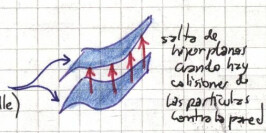
\includegraphics[scale=0.5]{images/1606329307.jpg} 
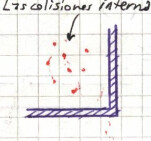
\includegraphics[scale=0.5]{images/1606329311.jpg}

Los de la izquierda son hiperplanos en $\Gamma$ (satisface Liouville); las colisiones internas (derecha)
generan movimiento en cada hiperplano que representa un volumen en $\Gamma$.
La densidad de estados $\rho$ decae exponencialmente. Tenemos dos fenómenos contrarios:
el decaimiento de $\rho$ y el crecimiento del número de estados a una energía

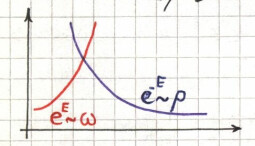
\includegraphics[scale=0.5]{images/1606329317.jpg}

Consideremos dipolos en campo magnético

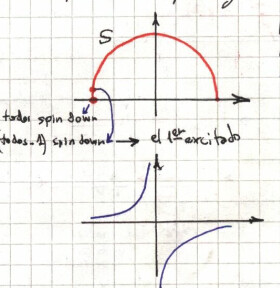
\includegraphics[scale=0.5]{images/1606329322.jpg}

La simetría de los dipolos up y down nos da la forma simétrica de la entropía $S$

Para las temperaturas tengo $T<0$ lo cual no puede medirse. No puedo medir con un termómetro; que
tiene un espectro continuo acotado.


\subsection{Gas ideal}

\[
	Q_N = \frac{(Vf(T))^N}{N!} \Rightarrow \Xi = \sum_{N=0}^\infty \frac{(zVf(t))^N}{N!} = \euler^{zVf(T)}
\]
\[
	\beta pV = \log (\Xi) = zVf(T) \qquad <N> = z \dpar{}{z} \log (\Xi) = zVf(T)
\]
y luego 
\[
	\beta pV = <N> \qquad \rightarrow \quad pV = <N> k T
\]
y recuperamos la ecuación de estado del gas ideal.


\subsection{Equivalencia canónico-gran canónico}

Para ver que con $ N \to \infty $ son equivalentes consideramos 
\[
	\kappa_T = \frac{1}{v} \left( -\dpar{v}{p} \right) < \infty \qquad \dpar{p}{v} < 0
\]

Pero en la coexistencia de una transición de fase de 1er orden se da 
\[
	\dpar{p}{v} = 0  \rightarrow \kappa_T \to \infty \text{ (sistema homogéneo) }
\]

La idea es ver que 
\begin{itemize}
 \item Dado $z$ existe $N$ tal que $ \Xi = \sum_N z^N Q_N(V,T) $
 \item Dado $N$ existe $z$ tal que $ \Xi = \sum_N z^N Q_N(V,T) $
\end{itemize}

Esto se comprueba. Además, si:
\[
	W (N) = z^N Q_N (V,T) \propto \text{ Prob. de que el sistema tenga $N$ partículas }
\]

XXX dibujos XXXX

En la transición de fase, donde $ \dpar{p}{v} = 0  $ todos los $ N $ son igual de probables porque
fluctúa la densidad. La $p$ se mantiene constante pero se varían los $ N_i $ de cada fase 'i'.


\subsection{Otra derivación del gran canónico}

Podemos derivar el gran canónico desde 
\notamargen{Es la probabilidad de hallar al sistema '1' en un estado con $ E_1, N_1 $.}
\[
	\text{Prob } \propto \Gamma_2(E-E_1, N-N_1)
\]
\[
	\log  \Gamma_2(E-E_1, N-N_1) \cong  \log \Gamma_2( E, N ) + \frac{1}{k} \left. \dpar{S(E,N)}{E} \right|_E(-E_1)
	+\frac{1}{k} \left. \dpar{S(E,N)}{N} \right|_N(-N_1)
\]
\[
	\cong \log \Gamma_2( E, N ) - \frac{E_1}{kT} + \frac{N_1\mu}{kT}
\]
\[
	\text{Prob } \propto \euler^{-\beta E}  \euler^{\beta \mu N}  = \euler^{-\beta E} z^N
\]
donde $T$ y $\mu$ son las asociadas al baño.
\notamargen{$\partial S/\partial E = 1/T$ y $\partial S/\partial N = -\mu / T$.}

Pensamos en $\eta$ copias del sistema; $n_{E_1N_1} = \# $ de sistemas con energía $E_1$ y $N_1$ partículas,
luego 
\[
	\sum_{\{ E_1, N_1 \}} n_{E_1N_1} = \eta \qquad \sum_{\{ E_1, N_1 \}} n_{E_1N_1}E_1 = n\bar{E}_1 \cong 
	\text{ Energía Total }
\]
\[
	\sum_{\{ E_1, N_1 \}} n_{E_1N_1} N_1 = \eta \bar{N}_1 \cong \text{ \# Total de partículas (no físico) }
\]
donde $ \bar{N}_1 $ es el número de medio.
\[
	\Omega\{ n_{E_1N_1} \} = \frac{\eta !}{\prod (n_{E_1N_1})!} \qquad \text{ combinatorio }
\]

La conbinación de mayor volumen será 
\[
	\log \Omega - \alpha \sum n E_1 - \beta_L \sum n N_1 = 0
\]
\[
	-\sum \left[ n\log n - n - \alpha n E_1 - \beta_L n N_1 \right] = 0
\]
\[
	-\sum n \left[ \log n - 1 - \alpha E_1 - \beta_L N_1 \right] = 0 
	\rightarrow \log(\tilde{n}) = 1 + \alpha E_1 + \beta_L N_1
\]
\[
	\tilde{n} \propto \euler^{\alpha E_1 + \beta_L N_1}
\]
que es el conjunto $n_{E_1N_1}$ de mayor volumen en $ \Omega $.

Esperaremos qeu con $ \eta\to\infty $ sea $<n_{E_1N_1}> \cong \tilde{n}_{E_1N_1} $.
Para determinar $\alpha, \beta$ usaremos 
\[
	\tilde{N} \cong <N> = \dpar{}{\beta_L}\left( \log \sum_{\{ E_1, N_1 \}} 
	\euler^{\alpha E_1 + \beta_L N_1} \right)
\]
\[
	\tilde{E} \cong <\Ham> =  \dpar{}{\alpha}\left( \log \sum_{\{ E_1, N_1 \}}
	\euler^{\alpha E_1 + \beta_L N_1} \right)
\]

% =================================================================================================
\section{Entropía de Gibbs}
% =================================================================================================

Sea $X$ extensiva mecánica,
\[
	S = k \log \Gamma (E,X) \qquad dU = TdS + Y dX, \; \frac{dS}{k} = \beta dU + \xi dX
\]
\notamargen{Donde $\beta Y = \xi $}
Consideramos un sistema en equilibrio donde fluctúan $E$ y $X$ (sistema en contacto con reservorios)

Refiriéndo al estado $ \nu $
\[
	P_\nu = \frac{ \euler^{-\beta E_\nu - \xi X_\nu } }{ \sum_\nu \euler^{-\beta E_\nu - \xi X_\nu } } =
	\frac{ \euler^{-\beta E_\nu - \xi X_\nu }}{\Theta}
\]
\[
	<E> = -\dpar{}{\beta} \log \Theta  \qquad <X> = -\dpar{}{\xi} \log \Theta 
\]
\notamargen{Caso $X=N$ $z\dpar{}{z} \cong \dpar{}{\beta \mu }$ }
\[
	d( \log \Theta ) = -<E> d\beta - <X> d\xi 
\]

Sea 
\[
	\Lag \equiv -k \sum_\nu P_\nu \log P_\nu =
	-k \sum_\nu P_\nu \log \left[ \euler^{-\beta E_\nu - \xi X_\nu } \Theta^{-1} \right]
\]
\[
	\Lag = \sum_\nu P_\nu k \log \Theta + k P_\nu \beta E_\nu + k P_\nu \xi X_\nu
\]
\[
	\Lag = k\log \Theta + k\beta <E> + k\xi <X>
\]
\[
	d\Lag = k\beta d<E> + k\xi d<X>
\]

Es una transformada de Legendre que toma $\log \Theta$ y la lleva a una función de $ <E>, <X> $
\[
	d\Lag = k \beta dE + k \beta Y dX = dS = \frac{1}{T}dE + \frac{Y}{T} dX 
\]
entonces $\Lag$ es la entropía $S$ (parecida al H de Boltzmann[?]).
\[
	\Lag = -k \sum_\nu P_\nu \log P_\nu 
\]
y $\nu$ son equiprobables
\[
	\Lag = -k \sum_\nu \frac{1}{\Gamma} \log \left( \frac{1}{\Gamma} \right) = 
	\sum_\nu \frac{k}{\Gamma} \log(\Gamma)
\]
y entonces
\[
	\Lag = k \log( \Gamma ) \equiv S.
\]

La entropía de Gibbs se reduce a la entropía de Boltzmann cuando los estados son equiprobables.

\begin{itemize}
 \item Microcanónico: requiere que ``cuente'' todos los estados.
 \item Canónico: me quito de encima la condición sobre la $E$.
 \item Gran canónico: me sacao de encima la condición sobre el número de partículas.
\end{itemize}

Pero las fluctuaciones de $E$ y $N$ van a cero con $N \to \infty$ y son equivalentes.


\subsection{Observación promedios}

\[
	<G> = \frac{\sum_N z^N G Q_N(V,T) }{\Xi} = \frac{\sum_N z^N \sum_\nu G(E_\nu, N, T) Q_N(V,T) }{\Xi}
\]
donde el último factor en la sumatoria es $<G>_{\text{CAN}} Q_N(V,T)$.

La parte crítica está en el pasaje de 
\[
	\sum_\nu \euler^{ -\beta E_\nu }
\]
a algún índice útil que permite realizar la sumatoria. En el caso de cuasipartículas, como osciladores, 
tenemos
\[
	\hat{H} = \sum_i^N \left( n_i + \frac{1}{2} \right) \hbar \omega_i 
\]
donde $ n_i $ es el número de fotones del oscilador i-ésimo. Los fonones cumplen el rol de partículas
\footnote{Porque podemos considerar que la $\sum$ se hace en niveles energéticos en lugar de entre osciladores
y tenemos un \# indeterminado de ``particulas'' (fonones) distribuidas en 'N' niveles energéticos.}
Un oscilador ddado puede tener en principio cualquier valor de energía (cualquier valor de $ n_i $) y esto 
independientemente de los otros $ N-1 $ osciladores. El número total de fonones del sistema
\[
	\sum_i^N n_i
\]
no es una constante del mismo con lo cual no hay vínculo. Entonces
\[
	\sum_\nu \qquad \rightarrow \qquad \sum_{n_1=0}^\infty \sum_{n_2=0}^\infty ... \sum_{n_\nu=0}^\infty
\]


\section{SUELTO: reubicar}

\[
	Z_N = \int d^{3N}q \prod_{i<j}^N (1+f_{ij}) \qquad \text{ integral configuracional }
\]
En realidad esta integral serán $ N(N-1)/2 $ integrales (N-grafos). Podemos factorizar los $ N(N-1)/2 $ grafos
en l-racimos teniendo en cuenta que se cumple
\[
	N = \sum_{l=1}^N ln_l,
\]
de forma que cada N-grafo dtermina un conjunto $ \{ m_l \} = (m_1,m_2, ..., m_N) $ de '$m_1$' 1-racimos, '$m_2$' 
2-racimos y '$m_N$' N-racimos. Por supuesto, un mismo conjunto $ \{ m_l \} $ determina muchos (en principio) N-grafos 
en función de la permutación de etiquetas.
\[
	\frac{N(N-1)}{2} \text{ N-grafos } \rightarrow M \text{ conjuntos } \{ m_l \}
\]
y la 
\[
	Z_N = \sum_1^{N(N-1)/2 } \text{ N-grafos } \quad \equiv \quad \sum_ {\{ m_l \}}' S(\{ m_l \})
\]
donde 
\[
	S(\{ m_l \}) = \prod_{l=1}^N \left( \sum \text{ l-racimos de l partículas }\right)^{m_l}
	\frac{N!}{ 1!^{m_1} 2!^{m_2} ..,N!^{m_N} m_1! m_2! ... m_N!}
\]
siendo la productoria entre todos los l-racimos posibles de l partículas y donde el combinatorio tiene en cuenta que 
habría que permutar entre las etiquetas de las $N$ partículas (pués la sumatoria contempla l-racimos de l partículas).

\[
	S(\{ m_l \}) = \frac{N!}{ 1!^{m_1} 2!^{m_2} ..,N!^{m_N} m_1! m_2! ... m_N!} \prod_{l=1}^N
	( l! \lambda^{3(l-1)}Vb_l )^{m_l} 
\]
\[
	S(\{ m_l \}) = N! \lambda^{3N} \prod_{l=1}^N \left( \frac{Vb_l}{\lambda^3}\right)^{m_l}\frac{1}{m_l!}
\]
\[
	Z_N = \sum_ {\{ m_l \}}' S(\{ m_l \})
\]
\[
	Q_N = \frac{1}{N! \lambda^{3N}} Z_N = \sum_ {\{ m_l \}}' \prod_{l=1}^N 
	\left( 	\frac{Vb_l}{\lambda^3}\right)^{m_l}\frac{1}{m_l!}
\]
\[
	\Xi = \sum_{N=0}^\infty z^N Q_N(V,T) = \sum_{N=0}^\infty z^N \sum_ {\{ m_l \}}' \prod_{l=1}^N 
	\left( 	\frac{Vb_l}{\lambda^3}\right)^{m_l}\frac{1}{m_l!}
\]
\[
	\Xi = \sum_ {m_1=0}^\infty ... \sum_ {m_N=0}^\infty   z^N \prod_{l=1}^N 
	\left( 	\frac{Vb_l}{\lambda^3}\right)^{m_l}\frac{1}{m_l!}
\]
donde hemos utilizado los resultados
\[
	z^N = z^{\sum_1^N l m_l } = \prod_1^N (z^l)^{m_l} \qquad 
	\prod_{l=1}^N \frac{(l!)^{m_l}}{1!^{m_1}...N!^{m_l}} = 1
\]
\[
	\prod_{l=1}^N  \lambda^{3lm_l} = \lambda^{3\sum_1^N lm_l} = \lambda^{3N}
\]

\[
	\Xi = \sum_ {m_1=0}^\infty ... \sum_ {m_N=0}^\infty   z^N \prod_{l=1}^N 
	\left( 	\frac{Vb_l}{\lambda^3}\right)^{m_l}\frac{1}{m_l!} = 
	\prod_{l=1}^N  \sum_ {m_1=0}^\infty \frac{1}{m_l!} \left( \frac{z^l Vb_l}{\lambda^3}\right)^{m_l} =
	\prod_{l=1}^N  \euler^{ \frac{z^l Vb_l}{\lambda^3} } 
\]
\[
	\beta pV = \log \Xi = \sum_l \frac{z^l V b_l}{\lambda^3} = \frac{V}{\lambda^3} \sum_l z^l b_l
\]
\[
	\begin{cases}
	\beta p = \frac{1}{\lambda^3} \sum_z^l b_l \\
	\frac{N}{V} = \frac{1}{\lambda^3} \sum_l z^l b_l
	\end{cases}
\]
que es la cluster-expansion.

\subsection{Integral configuracional y $Q_N(V,T)$}

Para un hamiltoniano usual
\[
	\Ham = \sum_i^N \frac{|\vec{p}_i|^2}{2m} + \sum_{i<j} V_{ij}(q_i) = K(\{ p_i \}) + V(\{ q_i \})
\]
\[
	Q_N(V,T) = \frac{1}{h^{3N}N!}\int d^{3N}p \int d^{3N}q \euler^{-\beta \Ham(\{ p_i,q_i \})} =
	\frac{1}{h^{3N}N!}\int d^{3N}p \euler^{-\beta K(\{ p_i \})}  \int d^{3N}q \euler^{-\beta V(\{ q_i \}) } 
\]
\[
	Q_N(V,T) = \frac{1}{\lambda^{3N}N!} \int d^{3N}q \euler^{-\beta V(\{ q_i \}) }  =
	\frac{1}{\lambda^{3N}N!} \: Z_N(V,T)
\]
donde $Z_N$ es la integral configuracional
\[
	\beta p = \frac{1}{\lambda^3} \sum_l z^l b_l  \qquad \frac{1}{v} = \frac{1}{\lambda^3} \sum_l lz^l b_l 
\]
\[
	\beta p v = \frac{ \sum_l z^l b_l }{ \sum_l l z^l b_l  }
\]
y el virial es 
\[
	\sum_{l=1} a_l(T) \left( \frac{\lambda^3}{v} \right)^{l-1} = \frac{ \sum_l z^l b_l }{ \sum_l l z^l b_l  }
\]
\[
	\sum_{l=1} a_l(T) \left( \sum_l l z^l b_l \right)^{l-1} \sum_l l z^l b_l = \sum_l z^l b_l 
\]
\[
	\sum_{k=1} a_k [ zb_1 + 2z^2b_2 ]^{k-1} (zb_1+2z^2b_2) \cong zb_1 + z^2b_2
\]
\[
	a_1(zb_1+2z^2b_2) + a_2(zb_1+2z^2b_2) (zb_1+2z^2b_2) \cong zb_1 + z^2b_2
\]
\[
	za_1b_1 + 2z^2a_1b_2 + a_2z^2b_1^2 + 4a_2z^3b_1b_2 + 4 a_2 z^4 b_2^2 \cong zb_1 + z^2b_2
\]
e igualando coeficientes de $ z $ tendremos 
\[
 	a_1b_1 = b_1 \quad \rightarrow \quad a_1 = 1
\]
\[
	2a_1b_2 + a_2b_1^2 = b_2  \quad \rightarrow \quad  a_2 = -\frac{b_2}{b_1^2} = -b_2
\]





% \bibliographystyle{CBFT-apa-good}	% (uses file "apa-good.bst")
% \bibliography{CBFT.Referencias} % La base de datos bibliográfica

\end{document}

	
		\documentclass[10pt,oneside]{CBFT_book}
	% Algunos paquetes
	\usepackage{amssymb}
	\usepackage{amsmath}
	\usepackage{graphicx}
	\usepackage{libertine}
	\usepackage[bold-style=TeX]{unicode-math}
	\usepackage{lipsum}

	\usepackage{natbib}
	\setcitestyle{square}

	\usepackage{polyglossia}
	\setdefaultlanguage{spanish}
	



	\usepackage{CBFT.estilo} % Cargo la hoja de estilo

	% Tipografías
	% \setromanfont[Mapping=tex-text]{Linux Libertine O}
	% \setsansfont[Mapping=tex-text]{DejaVu Sans}
	% \setmonofont[Mapping=tex-text]{DejaVu Sans Mono}

	%===================================================================
	%	DOCUMENTO PROPIAMENTE DICHO
	%===================================================================

\begin{document}

% =================================================================================================
\chapter{Gases clásicos ideales}
% =================================================================================================


% =================================================================================================
\section{Fluidos clásicos --reacomodar--}
% =================================================================================================

Empezamos con las funciones de distribución (en el ensamble canónico). Sabemos que
\[
	\left( \frac{\euler^{-\beta V}}{Z_N} \right)d^3q_1 d^3q_2 ... d^3q_N = 
	\text{ \# de microestados tales que '1' está en $\vec{q}_1$, etc. }
\]
donde los momentos están integrados y se cumple 
\[
	V = \sum_{i<j}^N v_{ij}.
\]
Pero ahora 
\begin{multline*}
	\left[ \int d^3q_{l+1} d^3q_{l+1} ... d^3q_{N} \frac{\euler^{-\beta V}}{Z_N} \right] d^3q_1 d^3q_2 ... d^3q_l 
	=\\
	\text{ \# de partículas tales que '1' está en $\vec{q}_1$, la 'l' en $q_l$ y las otras en cualquier parte } 
\end{multline*}

Como las partículas son indistinguibles agregamos 
\[
	\frac{N!}{(N-l)!} \left[ \int d^3q_{l+1} d^3q_{l+1} ... d^3q_{N} \frac{\euler^{-\beta V}}{Z_N} \right] 
	d^3q_1 d^3q_2 ... d^3q_l = \text{ \# de partículas ... } 
\]
y así definimos
\[
	\rho^{[1]}( q_1,...,q_l, V, T ) \equiv \frac{N!}{(N-l)!} \frac{1}{Z_N} \int d^{3N}q_{l+1} ...  d^{3N}q_N 
	\euler^{-\beta V}
\]
que es la función de distribución de $l$ cuerpos.
\[
	\rho^{[1]}( q_1, V, T ) = \frac{N}{Z_N} \int d^{3N}q_2 ...  d^{3N}q_N \euler^{-\beta V}
\]
y entonces
\[
	\int dq_1 \rho^{[1]}( q_1, V, T ) = N \qquad \text{ normalización }
\]
\notamargen{$ \rho^{[1]} = cte.$ entonces $N=\int dq_1 \rho^{[1]} $ y $N/V = \rho^{[1]} $, lo cual es muy razonable.}

Definimos 
\[
	\rho^{[l]} = \left( \frac{N}{V} \right)^l g^{[l]} \qquad g^{[l]} = \frac{\rho^{[l]}}{\rho^l} 
	\qquad N = \frac{N}{V} \int dq_1 g^{[1]}( q_1 )
\]
\notamargen{ $g^{[l]}$ es una especie de densidad relativa. }

\subsection{Análisis de $g^{[2]}(\vec{q}_1,\vec{q}_2)$}

Se puede medir mediante scattering de rayos X.
Con un potencial esférico
\[
	V(\vec{q}_1,\vec{q}_2) = V( |\vec{q}_1-\vec{q}_2| ) = V(q)
\]
donde $q$ es coordenada relativa  y entonces 
\[
	\rho^{[2]} = \left( \frac{N}{V} \right)^2 g^{[2]}( q_1, q_2 ) = 
	\left( \frac{N}{V} \right)^2 g( q )
\]
\[
	\int dq_1 dq_2 \rho^2 g^{[2]} = N(N-1) \qquad \qquad 4\pi \int dq \: q^2 \rho g(q) = N(N-1)
\]
\[
	4\pi \int dq q^2 \rho g(q) \cong N \qquad \text{ esféricas }
\]

Ahora $g(q)\rho^2$ da la probabilidad de que dada una partícula en 'O' tenga otra a distancia $q$. Es una probabilidad
conjunta.
\notamargen{ $\rho^{[2]} = \rho^{[2]}(q_1,q_2,V,T)$ pero en un gas ideal es 
$ \rho^{[1]}(q_1,V,T) \rho^{[1]}(q_2,V,T) $ lo que significa que no hay correlación.}
Los casos límite serán 
\begin{itemize}
	\item $q \to 0 \quad g \to 0 \quad $ Por la repulsión del carozo
	\item $q \to \infty \quad g \to 1  \quad $ Por el desvanecimiento del potencial (a gran distancia el sistema se 
ve 	homogéneo)
\end{itemize}

DIBUJO

Para un líquido da algo como esto. El valor de $ \sigma $ sería como la separación a primeros vecinos.

Para un sólido sería algo como esto (ver debajo), donde los picos están asociados a la separación entre primeros, segundos y
terceros vecinos.

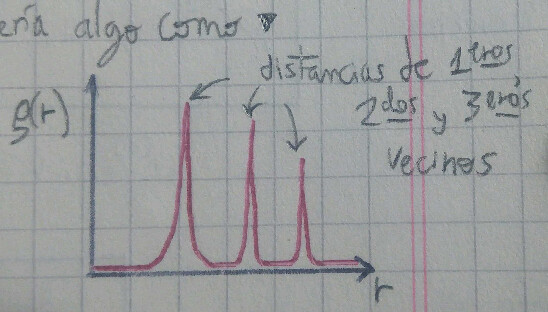
\includegraphics[scale=0.3]{images/1625623567.jpg}

\subsection{La termodinámica y $g(q)$}
\[
	\Ham = K(p) + V(q)
\]
\begin{multline*}
	E = <\Ham> = \frac{ \int d^{3N}p \int d^{3N}q \euler^{-\beta K - \beta V} (K+V) }
	{\int d^{3N}p \int d^{3N}q \euler^{-\beta K - \beta V}} = \\
	\frac{ \int d^{3N}p \int d^{3N}q \euler^{-\beta K - \beta V} K + \int d^{3N}p \int d^{3N}q \euler^{-\beta K - 
	\beta V} V }{ \int d^{3N}p \euler^{-\beta K } \int d^{3N}q \euler^{- \beta V} }
\end{multline*}
\[
	E = <K> + \frac{ \int d^{3N}q \euler^{-\beta V} V }{Z_N}
\]
\[
	-\dpar{}{\beta} \log Z_N = -\frac{1}{Z_N} \int d^{3N}q \euler^{-\beta V} (-V) = kT^2 \dpar{}{T}
\]
\[
	E = <K> + kT^2 \dpar{}{T}(\log Z_N)
\]
\[
	<V> =  \frac{ \int d^{3N}q \euler^{-\beta V} V }{Z_N} = 
	\frac{ \int d^{3N}q \euler^{-\beta \sum_{i<j}^N V_{ij} } \sum_{i<j}^N V_{ij} }{Z_N} =
	\sum_{i<j}^N \frac{ \int d^{3N}q \euler^{-\beta V } V_{ij} }{Z_N}
\]
\notamargen{La sumatoria en $ V_{ij} $ me la puedo sacar de encima.}
\[
	<V> = \frac{(N-1)N}{2} \frac{ \int d^{3N}q \euler^{-\beta V } V_{ij} }{Z_N}
\]
Metemos la expresión para $\rho^{[2]}$
\[
	\rho^{[2]} = \frac{N!}{(N-2)!} \frac{1}{Z_N} \int dq^3_3 ... d^3q_N \euler^{-\beta V}
\]
\[
	<V> = \frac{(N-1)N}{2} \int d^3q_1 d^3q_2 \left( 
	\frac{1}{Z_N} \int dq^3_3 ... d^3q_N \euler^{-\beta V}\right) V_{ij}
\]
\[
	<V> = \frac{(N-1)N}{2} \int d^3q_1 d^3q_2  \frac{(N-2)!}{N!}
	\rho^2 g^{[2]}(q_1,q_2) V_{12}
\]
\[
	<V> = \frac{1}{2} \int d^3q_1 d^3q_2 \rho^2 g^{[2]}(q_1,q_2) V_{12} =
	\frac{1}{2} \int 4 \pi dr r^2 \rho N  g(r) V(r)
\]
\[
	<V> = \frac{N^2}{2V} \int 4 \pi r^2 g(r) V(r) dr
\]
\[
	E = \frac{3}{2} NkT + \frac{N\rho}{2} \int_0^\infty 4 \pi r^2 g(r) V(r) dr
\]
siendo la integral del rhs la energía de interacción de una partícula con las demás sumada sobre todas las partículas.

La determinación de la presión se hace merced a 
\[
	p = -\dpare{A}{V}{N,T}, \quad A = -kT \log [Q_N(V,T)] 
	\qquad p = kT \frac{1}{Q_N} \dpar{}{V}[Q_N(V,T)]
\]
\notamargen{$A=T-TS$ y entonces $dA = dU-TdS-SdT = -pdV + \mu dN -SdT$ y entonces $p=-\partial A/\partial V$}
pero la dependencia del volumen se halla en la parte espacial de modo que 
\[
	p = kT \frac{1}{Z_N} \dpar{}{V}[ Z_N(V,T) ]  
\]
\[
	Z_N = \int d^{3N}q \euler^{\beta V}  = 
	\int_0^{V^{1/3}} \hspace*{-1em} dq_1 \int_0^{V^{1/3}} \hspace*{-1em} dq_2 ... \int_0^{V^{1/3}} 
	\hspace*{-1em} dq_{3N} \euler^{-\beta \sum_{i<j}^N V_{ij}(q_{ij}) }
\]
y cambiando variables con $ r = q/V^{1/3} $ que lleva a $ dq = V^{1/3} dr $
\[
	Z_N = V^N \int_0^1 d^{3N}r \euler^{-\beta \sum_{i<j}^N V_{ij}(V^{1/3}r_{ij}) }
\]


% \bibliographystyle{CBFT-apa-good}	% (uses file "apa-good.bst")
% \bibliography{CBFT.Referencias} % La base de datos bibliográfica

\end{document}

	
		\documentclass[10pt,oneside]{CBFT_book}
	% Algunos paquetes
	\usepackage{amssymb}
	\usepackage{amsmath}
	\usepackage{graphicx}
% 	\usepackage{libertine}
% 	\usepackage[bold-style=TeX]{unicode-math}
	\usepackage{lipsum}

	\usepackage{natbib}
	\setcitestyle{square}

	\usepackage{polyglossia}
	\setdefaultlanguage{spanish}
	



	\usepackage{CBFT.estilo} % Cargo la hoja de estilo

	% Tipografías
	% \setromanfont[Mapping=tex-text]{Linux Libertine O}
	% \setsansfont[Mapping=tex-text]{DejaVu Sans}
	% \setmonofont[Mapping=tex-text]{DejaVu Sans Mono}

	%===================================================================
	%	DOCUMENTO PROPIAMENTE DICHO
	%===================================================================

\begin{document}

% =================================================================================================
\chapter{Gases imperfectos}
% =================================================================================================


% =================================================================================================
\section{Cuánticos --reubicar}
% =================================================================================================

Ensamble de $ \mathcal{N} $ sistemas $(k=1,2,...,\mathcal{N})$. Cada uno tiene su estado descripto por 
\[
	\Psi^k(\vb{x},t), \qquad \qquad \hat{H} \Psi^k = i\hbar \dpar{\Psi^k}{t} \quad \forall k
\]

Si son estados puros entonces 
\notamargen{Todos son la {\it misma} combinación lineal de la base.}
\[
	\Psi^k = \sum_n a_n(t) \phi_n(\vb{x}) \qquad \{ \phi_n \} \text{ set ortonormal }
\]
Un estado puro es superposición coherente de una base 
\[
	i \hbar \dpar{}{t} a_m^k = \sum_n H_{mn}a_n^k
\]

El sistema k-ésimo puede describirse a partir de $ \Psi^k $ o bien a partir de los coeficientes $ \{ a_n \}$.

Definimos un operador de densidad,
\notamargen{Promedio en el ensamble de la interferencia cuántica entre $\phi_m$ y $\phi_n$. $p_k$ es la probabilidad
del estado $k$.}
\[
	\rho_{mn} \equiv \sum_{k=1}^{\mathcal{N}} p_k a_m^k (a_n^k)^*
\]
el cual proviene de 
\[
	\hat{\rho}_{mn} = \sum_{k=1}^{\mathcal{N}} p_k \Ket{\Psi^k}\Bra{\Psi^k}
\]
\notamargen{¿Y los índices $mn$ capo?}

Puede verse que se cumple
\[
	i \hbar \dot{\rho} = [ \hat{H}, \hat{\rho} ],  
\]
un teorema de Liouville cuántico.
 
Sea el valor medio de $ \hat{G} $
\[
	\braket{G}_{ENS} = \sum_{k=1}^{\mathcal{N}} p_k \braket{G}_k = 
	\sum_{k=1}^{\mathcal{N}} p_k \braket{\Psi^k|\hat{G}|\Psi^k}_k = 
	\sum_k p_k \int \sum_i a_i^{k*}\phi_i^* \hat{G}\sum_j a_j^k\phi_j dx
\]
\[
	\braket{G}_{ENS} = \sum_k p_k \sum_i \sum_j a_i^{k*}  a_j^k \int \phi_i^* G \phi_j dx =
	\sum_i \sum_j \left( \sum_k p_k a_i^{k*}  a_j^k \right) G_{ij}
\]
\[
	\braket{G}_{ENS} = \sum_i \sum_j \rho_{ij} G_{ij} = 
	\text{ Traza }(\hat{\rho}\hat{G}) = \sum_i [\rho G]_{ii}
\]

Ahora, si el conjunto $\{ \phi_n \}$ fuesen autoestados de $\hat{G}$ entonces 
\[
	\int dx \phi_i^* G \phi_j = \int dx \phi_i^* \phi_j g_j = \delta_{ij} g_j = g_i
\]
\[
	\braket{G}_{ENS} = \sum_k p_k \sum_i a_i^{k*}  a_i^k g_i = 
	\sum_k p_k \sum_i |a_i^k|^2 g_i
\]

La matriz densidad $\hat{\rho}$ se define de modo que sus elementos $\rho_{ij}$ resultan 
\[
	\braket{\phi_i|\hat{\rho}|\phi_j} = \sum_{k=1}^{\mathcal{N}} p_k \braket{\phi_i|\Psi^k} \braket{\Psi^k|\phi_j} =
	\sum_{k=1}^{\mathcal{N}} p_k \int dx \phi^*_i \sum_l a_l^k \phi_l \int dx' \phi_j \sum_m a_m^{k*} \phi_m^*
\]
\[
	\braket{\phi_i|\hat{\rho}|\phi_j} = 
	\sum_{k=1}^{\mathcal{N}} p_k \sum_l \sum_m a_l^k a_m^{k*} \int dx \phi^*_i \phi_l \int dx' \phi_j \phi_m^* =
	\sum_{k=1}^{\mathcal{N}} p_k \sum_l \sum_m a_l^k a_m^{k*} \delta_{il}\delta_{jm}
\]
\[
	\rho_{ij} = \sum_k p_k a_i^k a_j^{k*}
\]

El primer postulado de la QSM es asegurarse de que $\rho_{ij} \propto \delta_{ij} $, es decir que
EN PROMEDIO no hay correlación entre funciones $\{ \phi_i \}$ para diferentes miembros $k$ del ensamble.
El elemento $\rho_{ij}$ es el promedio en el ensamble de la interferencia entre $\phi_i$ y $\phi_j$.


En la práctica los ensambles serán mezcla, una superposición de estados puros pero incoherente, de modo
que 
\notamargen{Es muy difícil preparar un ensamble puro.}
\[
	\hat{\rho} = \sum_{k=1}^{\mathcal{N}} p_k \Ket{\Psi^k}\Bra{\Psi^k} \qquad p_k \geq 0 \quad \sum_k p_k = 1 
\]
donde $p_k$ serán las {\it abundancias relativas} de los estados puros $\Psi^k$.

Para un ensamble puro sería
\[
	\hat{\rho} = \Ket{\Psi}\Bra{\Psi}
\]
donde no hay supraíndice $k$ puesto que todos son el mismo estado.

Un estado puro puede escribirse 
\[
	\Psi^k = \sum_n a_n \phi_n, \quad \text{ o bien }\quad \Ket{\Psi^k} = \sum_n a_n \Ket{\phi_n}
\]
y sabemos que el valor de expectación será
\[
	\braket{A}_k = \braket{\Psi^k|\hat{A}|\Psi^k} = \int dx \Psi^{k*} A \Psi^k
\]

Un estado mezcla será en cambio 
\be
	\Ket{\xi} \cong \sum_n p_n\Ket{\phi_n}
	\label{estado_mezcla}	
\ee
donde $\sum_n p_n =1$ y $p_n \in \mathbb{R}>0$. Pero $\Ket{\xi} $ no es un estado de sistema como $\Psi^k$ pués
\be
	\Ket{\xi} \neq \sum_n c_n\Ket{\phi_n}
	\label{falso_mezcla}
\ee
no hay cambio de base que lleve \eqref{estado_mezcla} al miembro derecho de \eqref{falso_mezcla}.
Entonces
\[
	\braket{A}_\xi \neq \braket{\xi|\hat{A}|\xi}
\]

Pero como en la práctica lo que se tiene son estados mezcla, la matriz de densidad $\hat{\rho}$ permite trabajar
con ellos tranquilamente.

Sea que evaluamos el valor medio de $ \hat{G} = \hat{\Ham} $ que será la energía $\braket{E}$ en autoestados de 
$ \hat{\Ham} $.
\[
	\braket{\hat{\Ham}}_{ENS} = \braket{E} = \sum_k p_k \sum_i \sum_j a_i^{k*} a_j^k \int \phi_i^* \phi_j E_j =
	\sum_k p_k \sum_j a_j^{k*} a_j^k E_j
\]
\[
	\braket{E} = \sum_k p_k \sum_j a_j^{k*} a_j^k E_j = \sum_j \left( \sum_k p_k a_j^{k*} a_j^k \right) E_j =
	\sum_j \rho_{jj} E_j
\]

Se tiene que $ \hat{\rho} $ es diagonal para un operador $\hat{G}$ tal que utilizamos la base de autoestados.

Querremos que esto valga para cualquier base entonces necesitaremos que las fases sean números aleatorios:
\[
	\rho_{ij} = \sum_k^{\mathcal{N}} p_k a_i^{k*} a_j^k = 
	\sum_k^{\mathcal{N}} p_k | a_i^k | | a_j^k |\euler^{i( \theta_i^k - \theta_j^k )}
\]
y asi además son equiprobables (microcanónico) los estados base accesibles,
\[
	p_k = \frac{1}{\mathcal{N}} \qquad \text{ y } \qquad |a^k_i| = |a_i| \quad \forall k
\]
y asimismo pedimos que para cada miembro del ensamble la amplitud sea la misma, se tiene 
\[
	\rho_{ij} = | a_i | | a_j | \frac{1}{\mathcal{N}} \sum_k^{\mathcal{N}} \euler^{i( \theta_i^k - \theta_j^k )}
	= | a_i | | a_j | \delta_{ij}
\]
donde se han usado fases al azar, de modo que 
\[
	\rho_{ij} = | a_i |^2 \delta_{ij} = \rho_i \delta_{ij}
\]
\notamargen{Esto no está consistente: colapsas la delta o no, papi?}
y entonces 
\[
	\begin{cases}
	 \rho_i = \displaystyle{ \frac{1}{\Gamma} }\\
	 \rho_i = 0
	\end{cases}
\]

Entonces $ \rho_i $ será la probabilidad del estado de base $ \phi_i $. Se sigue que el operador densidad del
microcanónico puede escribirse 
\[
	\hat{\rho} = \sum_i | a_i |^2 \Ket{\phi_i}\Bra{\phi_i}
\]
de manera que es una superposición incoherente de estados de la base $\{ \phi_i \}$
\[
	\hat{\rho} = \sum_i \rho_i \Ket{\phi_i}\Bra{\phi_i}
\]
y al final del día
\[
	\rho_{kl} = \braket{ \phi_k | \hat{\rho} | \phi_l } = \sum_i \rho_i 
	\braket{ \phi_k | \phi_i }  \braket{ \phi_i | \phi_l } = \sum_i \rho_i \delta_{ki} \delta_{il} = 
	\rho_k \delta_{kl}
\]

\[
	\Omega = 1 \text{ ensamble puro } \qquad \qquad S = k\log \Omega = 0
\]
\[
	\rho_{mn} = \frac{1}{\mathcal{N}} \sum_k^{\mathcal{N}} a_m^{k*} a_m^k = a_m a_n^* 
\]
si es la misma $\Psi \forall k$ el sistema se halla en una combinación lineal de $\phi_n$, o bien
\[
	\rho_{mn} = |a_m|^2 \delta_{mn}
\]
el sistema se halla en un único autoestado $ \phi_n $

\[
	\Omega > 1 \text{ ensamble mezcla }
\]

\subsection{Resumen formalismo}

\[
	\rho_{ij} = \rho_i \delta_{ij}
\]
\[
	\rho_i = \frac{1}{\Omega} \qquad \text{ Microcanónico }
\]
\[
	\rho_i = \frac{\euler^{-\beta E_i}}{Q_N(V,T)}  \qquad  \text{ Canónico }
\]
\[
	\rho_i = \frac{\euler^{-\beta E_i + \beta \mu N_i }}{\Xi(z,V,T)}  \qquad  \text{ Gran canónico }
\]

\[
	\hat{\rho} = \sum_i \Ket{ \phi_i } \rho_i \Bra{ \phi_i } \qquad \qquad \text{ Traza }(\hat{\rho} ) =
	1 \text{ bien normalizado }
\]
\[
	\hat{\rho} = \frac{1}{\Omega} \sum_i^{\text{ACC}} \Ket{ \phi_i } \Bra{ \phi_i } = 
	\frac{1}{\Omega} \hat{\mathbb{1}}^{\text{ACC}}  \qquad \text{ Tr }(\hat{\rho} ) = 1 
\]
donde $ \hat{\mathbb{1}}^{\text{ACC}}  $ es una indentidad con 0 para los sitios de la diagonal donde no hay
estado accesible. Luego $ \text{ Traza }(\hat{\mathbb{1}}^{\text{ACC}})  = \Omega $. Para los otros dos casos,
\[
	\hat{\rho} = \frac{\euler^{-\beta E_i}}{Q_N(V,T)}  \sum_i^{\text{ACC}} \Ket{ \phi_i } \Bra{ \phi_i } = 
	\frac{\euler^{-\beta E_i}}{Q_N(V,T)} \hat{\mathbb{1}}^{\text{ACC}} 
	\qquad \text{ Tr }(\hat{\rho} ) = \frac{1}{Q_N} \text{ Tr }( \euler^{-\beta E_i} \hat{\mathbb{1}}^{\text{ACC}} )
\]
\[
	\hat{\rho} = \frac{\euler^{-\beta E_i + \beta \mu N_i }}{\Xi(z,V,T)} 
	\sum_i^{\text{ACC}} \Ket{ \phi_i } \Bra{ \phi_i } = 
	\frac{\euler^{-\beta E_i + \beta \mu N_i }}{\Xi(z,V,T)} \hat{\mathbb{1}}^{\text{ACC}} 
	\qquad \text{ Tr }(\hat{\rho} ) = 
	\frac{1}{\Xi} \text{ Tr }( \euler^{-\beta E_i + \beta \mu N_i } \hat{\mathbb{1}}^{\text{ACC}} ) 
\]

El conteo de estados se hace cuánticamente de modo que no hay paradoja de Gibbs. Los estados accesibles en el
microcanónico $ (\Omega) $ son tales que sus probabilidad es 
\[
	| a_i |^2 = \frac{1}{\Omega} \quad \forall i \text{ accesible }
\]
Serán aquellos de la base $ \{ \phi_i \} $ en cuestión tales que la energía resulte vale entre $E$ y $E+\Delta E$.

Los dos postulados
\begin{itemize}
 \item i) Equiprobabilidad
 \item ii) Fases al azar
\end{itemize}
aseguran que no hay correlación entre las funciones $ \{ \phi_i \} $ (en promedio).


% =================================================================================================
\section{Gases reales}
% =================================================================================================

Función canónica de un gas real. Surge una integral configuracional
\[
	Z_N =  \int d^3q_1 ... d^3q_N \euler^{ - \beta \sum_{i<j} V_{ij} }
\]
En el gran canónico tenemos $ \Xi( Z_N ) $. Potencial de Lenard-Jones
\[
	\frac{1}{r^{12}} - \frac{1}{r^{6}}
\]

Definimos $ f_{ij} = \euler^{-\beta V_{ij}} - 1 $ y expresamos todo en términos de $ f_{ij} $.
Esta última tiene el mismo rango que el potencial de interacción.
De alguna manera esto que haremos es un desarrollo en serie del potencial de interacción.

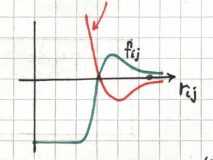
\includegraphics[scale=0.5]{images/1606329591.jpg}

Estudiamos con los N-grafos.

Consideramos un hamiltonianao
\[
	H = \sum_i^N \frac{ p^2 }{2m} + \sum V_{ij},
\]
donde $V_{ij}$ depende de $|r_i-r_j|$. Es un modelo clásico pero consideramos interacción.
La función de partición no se factoriza como el producto de funciones de una partícula justamente
debido a la interacción.

Metemos grafos ahora y llegaremos a una expresión para los coeficientes del virial.
El gas real lo estudiamos clásicamente, entonces 
\[
	Q_N = \frac{1}{N! h^{3N} } \int  d^{3N}q d^{3N}p  \euler^{ - \beta H(p,q) }
\]
si bien aparece $h$ (constante de Planck) no hablamos de funciones de onda; como sí sucede en una
expansión cuántica.
Se integra en los momentos y resulta
\[
	Q_N = \frac{1}{N! \lambda^{3N} } \int  d^{3N}q  \euler^{ - \beta \sum_{i<j} v_{ij} }
\]
donde $\lambda$ absorbe muchas constantes. Luego,
\[
	Q_N(V,T) = \frac{ Z_N }{ N! \lambda^{3N}},
\]
con $ Z_N $ la función de partición o integral configuracional.

El kid de la cuestión será hallar expresión para $Z_N$ que sea manejable. Pasaremos al gran canónico
\[
	\Xi(z,V,T) = \sum_{N=0}^\infty \: \Frac{z}{\lambda^3}^N \frac{ Z_N }{ N! }
\]
y usaremos la definición $f_{ij}$ que es de Mayer (1937) y vemos que sucede que 
\begin{itemize}
 \item $f_{ij}=0$ si $v_{ij}=0$
 \item No diverge
 \item $f_{ij} \sim 0$ con $r \gg r_0 $
 \item $f_{ij} \approx 0$ con $ k T \gg v_{ij}$ (altas temperaturas)
\end{itemize}

Todo esto parece razonable para los límites conocidos

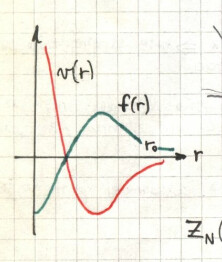
\includegraphics[scale=0.4]{images/1606337067.jpg}

La integral configuracional es un producto entre números de pares de partículas posibles
\[
	Z_N = \int  d^{3N}q \prod_{i<j} ( 1 + f_{ij} ),
\]
la cual tendrá $ (N-1)N/2 $ productos y $ 2^{N(N-1)/2} $ términos sumando de modo que serán esa cantidad
de integrales
\notamargen{Cada grafo puede verse en una matriz de adyacencias $M_{ij}$}
\begin{center}
\begin{tabular}{cc}
N=2 $ \to $ & $1$ producto y $2^1$ términos \\
N=3 $ \to $ & $3$ productos y $2^3=8$ términos \\
N=4 $ \to $ & $6$ productos y $2^6=64$ términos \\
N=10 $ \to $ & $45$ productos y $2^{45} \cong 3.5\cdot 10^{13}$ términos 
\end{tabular}
\end{center}
O sea que la intgral es una cosa del tipo 
\[
	Z_N = \int d^{3N}r \left[ 1 + (f_{12} + f_{13} + f_{23} + ... )
	+ ( f_{12} f_{13} + f_{12} f_{11} + ... ) + ... \right]
\]
y para hacer esta cuenta se asocia una integral con un grafo de $N$ partículas.

Por ejemplo tenemos un grafo de cuatro partículas y un grafo que se factoriza porque hay partes
disconexas

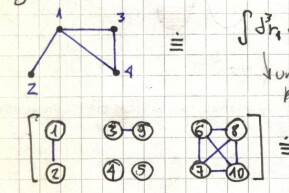
\includegraphics[scale=0.4]{images/1606337071.jpg}

que representan un 4-grafo
\[
	\int d^3r_1  d^3r_2 d^3r_3 d^3r_4 f_{12} f_{13} f_{34} f_{14},
\]
y un 10-grafo
\[
	\int d^3r_1 ... d^3r_{10} f_{39} f_{67} f_{68} f_{12} ...
\]

La factorización de este lleva a 

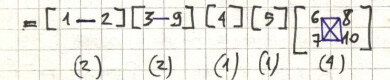
\includegraphics[scale=0.4]{images/1606337077.jpg}

donde cada uno es un {\it cluster} (racimo). Un $\ell-$cluster es un grupo de $\ell$ partículas que están
conectadas de modo que no se puede descomponer.

Cada grafo puede descomponerse en clusters y la función de partición puede epxresarse como la suma
de todos los posibles distintos grafos donde cada grafo puede factorizarse en clusters.

Es conveniente definir entonces una integral de cluster (racimo) que son las $b_\ell$



Cada uno de los N-grafos (integrales) puede factorizarse en l-racimos (l-grafo conexo).
\notamargen{Cada integral puede verse como un grafo. Anoté que esto puede verse bien
del libro de Pathria.}

La forma de asignar los índice será:
\[
	\frac{ N! }{[ (1!)^{m_1} \: (2!)^{m_1} \: ... ] m_1! \: m_2! \: ...}
\]
donde el corchete son permutaciones en el racimo y lo otro son permutaciones entre racimos.
Al final del día será,
\[
	\frac{PV}{kT} = \frac{ \sum \: z^\ell b_\ell }{ \sum \: \ell z^\ell b_\ell  }.
\]

Un dado N-grafo, por ejemplo

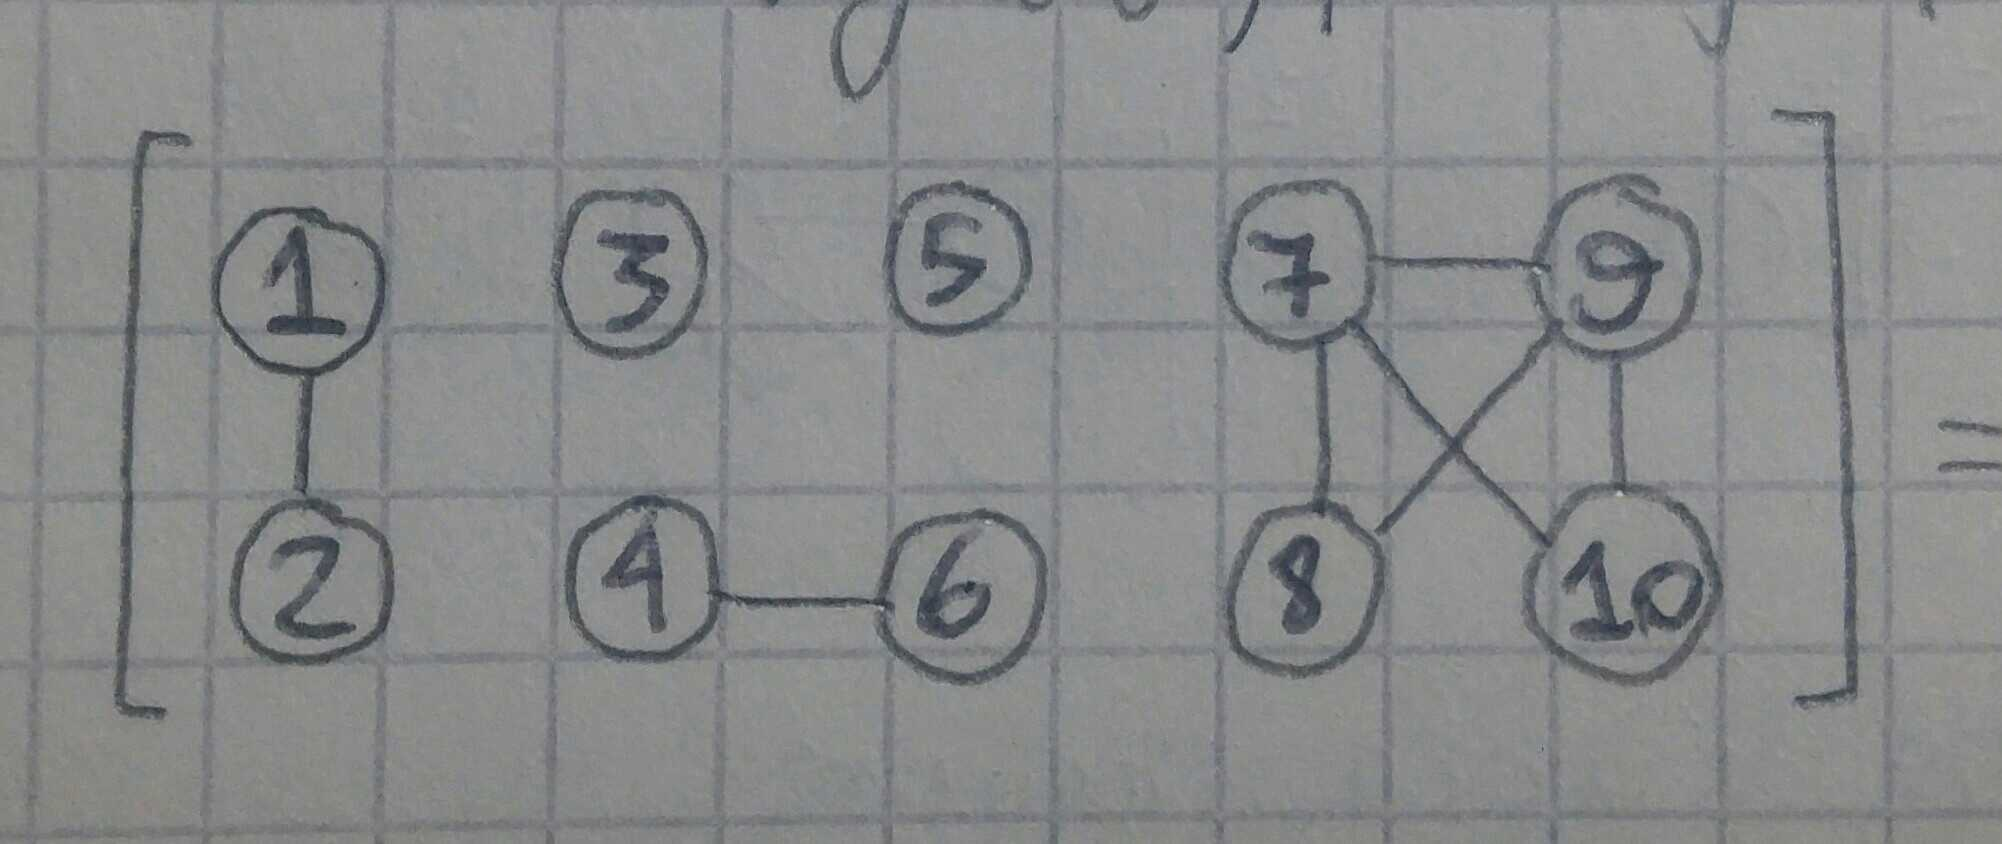
\includegraphics[scale=0.1]{images/1625626570456.jpg}
\begin{multline*}
	\int d^3r_1 d^3r_2 f_{12} \int d^3r_3  \int d^3r_4 d^3r_6 f_{46} \int d^3r_5 \times  \\
	\int d^3r_7 d^3r_8 d^3r_9 d^3r_{10} f_{78} f_{79} f_{710} f_{89} f_{910} 
\end{multline*}
tiene dos 1-racimo, dos 2-racimos y un 4-racimo.

\notamargen{Términos $f_{ij}$ son los links en el lenguaje de grafos.}
Un dado l-racimo tendrá al menos l-1 términos $f_{ij}$ para asegurar la conexión. El máximo será $l(l-1)/2$.
Se cumple 
\be
	N = \sum_{l=1}^N  \; l \cdot m_l \quad \text{ suma en racimos }
	\label{constraint}
\ee
siendo $l$ el número de partículas del racimo y $m_l$ el número de l-racimos y sujeta a
\[
	N = 1 \cdot 2 + 2 \cdot 2 + 4 \cdot 1 = 10 \qquad  \{ m_l \} = ( 2,2,0,1,0,0,0,0,0,0 )
\]

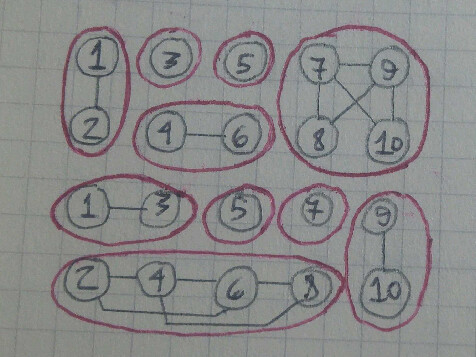
\includegraphics[scale=0.4]{images/1625625417.jpg}

Claramente separando en racimos cuento las partículas con \eqref{constraint}.

\notamargen{Cada N-grafo se divide en varios l-racimos. Un l-racimo tendrá de 1 a N partículas.}


Pero el set $ \{ m_l \} $ tiene degeneración pues es equivalente a este otro arreglo de racimos.

Se definen las integrales de racimo como 
\[
	b_l = \frac{1}{l! \lambda^{3l-3} V} \left[ \text{ suma de todos los l-racimos posibles }\right]
\]
donde sumar los l-racimos es en todas las configuraciones de l-bolas conexas DIBUJITO.
\[
	b_1 = \frac{1}{1! \lambda^0 V} \int d^3r_1 \leftarrow \sum \boxed{1} 
\]
\notamargen{Cambiar los boxed por circled!!!}
\[
	b_2 = \frac{1}{2! \lambda^3 V} \int d^3r_1 d^3r_2  f_{12} \leftarrow \sum \boxed{1} -- \boxed{2}
\]
\begin{multline*}
	b_3 = \frac{1}{3! \lambda^6 V} \int d^3r_1 d^3r_2 d^3r_3 (f_{12}f_{23} + f_{12}f_{13} + f_{13}f_{23}+
	f_{12}f_{13}f_{23} ) \\
	\leftarrow \sum_{\text{ perm. etiqu. }} \left[ \; \boxed{\phantom{a}}-\boxed{\phantom{a}} + 
	\boxed{\phantom{a}}-\boxed{\phantom{a}}-\boxed{\phantom{a}} \; \right]
\end{multline*}

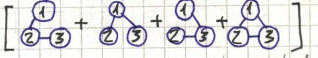
\includegraphics[scale=0.4]{images/1606337083.jpg}

Un par de cosas. Podemos definir un $b_\ell$ especial tal que 
\[
	\text{\sout{b}}_\ell(T) \equiv \lim_{V\to\infty} b_\ell(V,T) = \text{ finito }
\]
Además el $b_2$ se puede referir a coordenadas del centro de masa y así resulta
\[
	b_2 = \frac{1}{2! \lambda^3 V} \int d^3r_{12} f_{12}.
\]

Sea $ S( \{ m_l \} ) $ la suma de todos los l-racimos compatibles con el conjunto $ \{ m_l \}$
\[
	S( \{ m_l \} ) = \sum_{\text{ perm. conectores. }} \left[ \boxed{ \phantom{a} } \right]^2 \cdot 
	\left[ \boxed{ \phantom{a} }-- \right]^2 \left[ \boxed{ \phantom{a} } ---- \right]^1
\]
donde los conectores se permutan dentro de cada racimo.
\[
	Z_N = \int d^3q_1 d^3q_2 ... d^3q_N \: ( 1 + f_{12} + f_{13} + ... + f_{12}f_{13} + ... )
\]

Tenemos $ 2^{N(N-1)/2} $ integrales
\[
	Z_N = \int d^3q_1 1 + \int d^3q_2 f_{12} + ... + \int d^3q_N f_{12}f_{13} 
\]
Cada integral es un N-grafo (N bolas unidas por un número $m$ de links ($m$ es igual al número de $f_{ij}$)).

Cada N-grafo se factoriza en l-racimos y se puede escribir 
\[
	N = \sum_{l=1}^N  \; l \cdot m_l \quad \text{ suma en racimos }
\]
siendo $l$ el número de partículas en el racimo $l$ y $m_l$ el número de l-racimos. 
El conjunto $ \{ m_l \} $ es la distribución de l-racimos de un grafo
\[
	1. \text{ es } \{ m_l \} = ( N, 0, 0 , ..., 0 ) \qquad \text{ tiene $N$ 1-racimos }
\]
\[
	2.  \{ m_l \} = ( N-2, 1, 0 , ..., 0 ) \qquad \text{ tiene $N-2$ 1-racimos y $1$ 2-racimo }
\]
\[
	3. \{ m_l \} = ( N-3, 0, 1 , ..., 0 ) \qquad \text{ tiene $N-3$ 1-racimos y $1$ 3-racimo }
\]
\notamargen{ \[ N = N\cdot 1 \] \[ N = (N-2)\cdot 1 + 1 \cdot 2 \] \[ N = 1\cdot(N-3) + 3\cdot 1\]}

Sea $ S( \{ m_l \} ) $ la suma de todos los l-racimos compatibles con un conjunto $ \{ m_l \}$ dado,
\[
	S( \{ m_l \} ) = \sum_{\text{ perm. conectores. }} \left[ \boxed{ \phantom{a} } \right]^{m_1} \cdot 
	\left[ \boxed{ \phantom{a} }-- \right]^{m_2} \left[ \boxed{ \phantom{a} } ---- \right]^{m_3} \times ...
\]



Por ejemplo, para $m_3=2$ (dos 3-racimos)

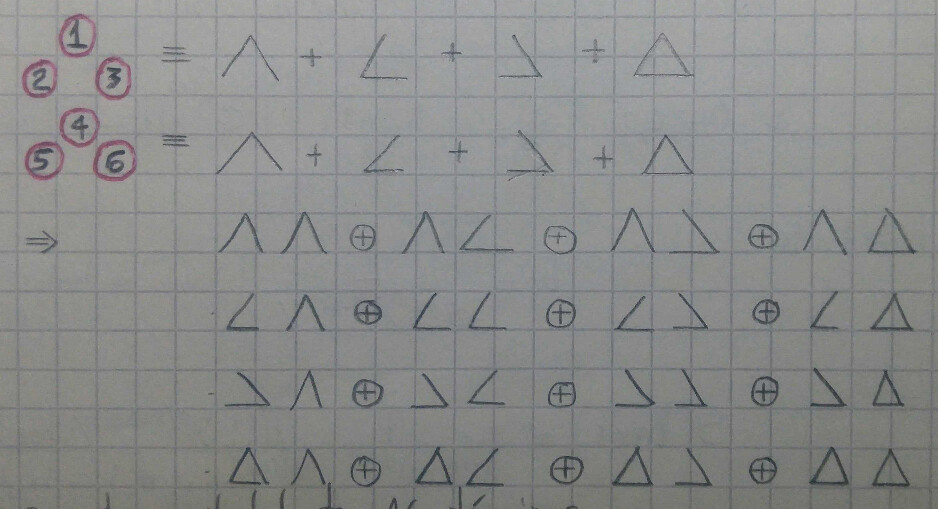
\includegraphics[scale=0.35]{images/1625625437.jpg}

lo que da un total de 16 términos.

Esto da el número de formas de construir un 6-grafo compuesto de dos 3-racimos

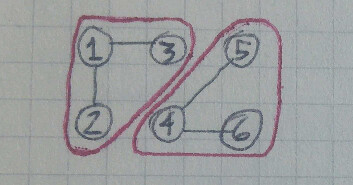
\includegraphics[scale=0.35]{images/1625625468.jpg}

Cada set $ \{ m_l \} $ define un conjunto de $ R = \sum m_l $ racimos correspondiente a un conjunto de 
N-grafos. Así:
\[
	\{ m_l \} = ( N-2, 1, 0, ..., 0 )
\]
representa

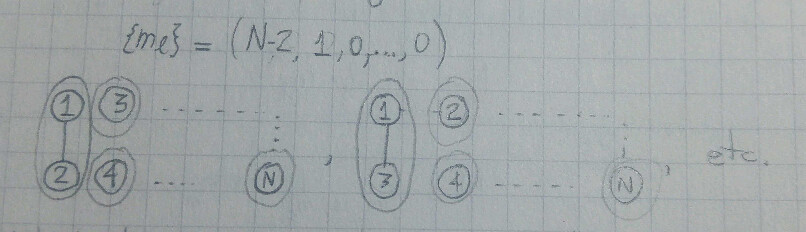
\includegraphics[scale=0.35]{images/1625625496.jpg}

una gran cantidad de N-grafos dada por permutar etiquetas. Pero si quiero economizar cuentas similares consideraré
un factor 
\[
	\frac{1}{ 1!^{m_1} 2!^{m_2} 3!^{m_3} ... N!^{m_N} }
\]
por permutaciones de índices en cada racimo 
\[
	\frac{1}{ m_1! m_2! ... m_N! }
\]
por permutaciones de índices entre racimos iguales.

Para el ejemplo es 
\[
	\frac{1}{1!^{N-1} 2!^1} \frac{1}{(N-2)! 1!}
\]
Entonces
\[
	S( \{ m_l \} ) = \frac{1}{ 1!^{m_1} 2!^{m_2} 3!^{m_3} ... N!^{m_N} } \frac{1}{ m_1! m_2! ... m_N! }
	\left[ \boxed{ \phantom{a} } \right]^{m_1} \times \left[ \boxed{ \phantom{a} }-- \right]^{m_2} \times ...
\]
\[
	S( ( N-2, 1, 0, ..., 0 ) ) = \frac{ N(N-1) }{2!}
	\left[ \boxed{ \phantom{a} } \right]^{m_1} \times \left[ \boxed{ \phantom{a} }-- \right]^{m_2} \times
	\left[ \boxed{ \phantom{a} } ---- \right]^{m_3} \times ...
\]

Recordando 
\[
	b_l = \frac{ 1 }{ l! \lambda^{3(l-1)} V }\cdot ( \text{ Suma de todos los l-racimos } )
\]
será 
\[
	S( \{ m_l \} ) = \frac{N!}{ 1!^{m_1} 2!^{m_2} 3!^{m_3} ... N!^{m_N} } \: \prod_{l}^N \: 
	\frac{ ( l! \lambda^{3(l-1)} V \: b_l )^{ m_l } }{ m_1! m_2! ... m_N! }
\]
\[
	S( \{ m_l \} ) = N! \: \prod_{l}^N \: 
	\frac{ ( \lambda^{3(l-1)} V \: b_l )^{ m_l } }{ m_1! m_2! ... m_N! }
\]

Luego
\[
	Z_N = \sum_{\{ m_l \} } ' S( \{ m_l \} ) = N! \lambda^{3N}  \sum_{\{ m_l \} }' \prod_{l}^N 
	\frac{1}{m_l!} \Frac{ V \: b_l }{ \lambda^3 }^{m_l}
\]
\[
	Q_N = \frac{1}{N! \lambda^{3N}} Z_N = 
	\sum_{\{ m_l \} }' \prod_{l}^N \frac{1}{m_l!} \Frac{ V \: b_l }{ \lambda^3 }^{m_l}
\]
\[
	\Xi = \sum_{N=0}^\infty z^N Q_N =  \sum_{m_1=0}^\infty \sum_{m_2=0}^\infty ...  \sum_{m_N=0}^\infty
	z^N \prod_{l}^N \frac{1}{m_l!} \Frac{ V \: b_l }{ \lambda^3 }^{m_l}
\]
\[
	\Xi = \sum_{m_1=0}^\infty \sum_{m_2=0}^\infty ...  \sum_{m_N=0}^\infty
	\prod_{l}^N \frac{1}{m_l!} \Frac{ z^l V \: b_l }{ \lambda^3 }^{m_l}
\]
\[
	\Xi = \prod_{l=1}^N \sum_{m_l=0}^\infty \frac{1}{m_l!} \Frac{ z^l V \: b_l }{ \lambda^3 }^{m_l}
	= \prod_{l=1}^N \euler^{ \frac{ z^l V \: b_l }{ \lambda^3 } }
\]
\[
	\log \Xi = \sum_{l=1}^N \log\left( \euler^{ \frac{ z^l V \: b_l }{ \lambda^3 } } \right) =
	\sum_{l=1}^N  \frac{ z^l V \: b_l }{ \lambda^3 }
\]
de modo que 
\[
	\beta p = \frac{ 1 }{ \lambda^3 } \sum_{l=1}^N  z^l b_l .
\]
	
\[
	b_1 = \frac{1}{1!\lambda^{3(1-1)}V} \int d^3r = \frac{V}{\lambda^0 V} = 1
\]
\[
	b_2 = \frac{1}{2\lambda^3 V} \int d^3r d^3r' f_{rr'} = \frac{1}{2\lambda^3 V} \int d^3r \int d^3u f_u
\]
\notamargen{$r-r'= u$ y entonces $-dr'= du$.}

Tenemos, una vez más,
\[
	\Xi(z,V,T) = \euler^{ \sum_{\ell=1}^\infty \: b_\ell z^\ell V / \lambda^3 }
\]
y considerando el límite termodinámico tenemos
\[
	\frac{P}{kT} = \frac{1}{\lambda^3} \sum_{\ell=1}^\infty \: \text{\sout{b}}_\ell z^\ell
	\qquad \qquad 
	\frac{1}{v} = \frac{N}{V} = \frac{1}{\lambda^3} \sum_{\ell=1}^\infty \: \ell \: \text{\sout{b}}_\ell z^\ell
\]

desde las cuales obtenemos (también en función de la densidad)
\[
	\frac{Pv}{kT} = \sum_{\ell=1}^\infty \: a_\ell(T) \Frac{\lambda^3}{v}^{\ell-1}
	= \sum_{\ell=1}^\infty \: B_\ell(T) \Frac{1}{v}^{\ell-1}
\]
siendo $ a_\ell(T), B_\ell$ coeficientes del virial. Luego, algunos coeficientes son
\[
	a_1 = \text{\sout{b}}_1 = 1 \qquad 
	a_2 = -\text{\sout{b}}_2 = \frac{2\pi}{\lambda^3} \int_0^\infty \: ( 1 - \euler^{v(r)/kT} ) \: r^2 \: dr
	\qquad
	B_2 = a_2 \lambda^3
\]
y
\[
	\frac{Pv}{kT} = \begin{cases}
	                 1 + B_2 f + ... \\
	                 1 + a_2 \Frac{\lambda^3}{v} + ... 
	                \end{cases}
\]
En general nuestros ejercicios apuntarán a calcular el segundo coeficiente del virial.

\subsection{Algún ejemplo particular}

Sea un sistema de esferas rígidas (potencial esférico)
\[
	f_u = \euler^{-\beta V_u} - 1 = \begin{cases}
	                                 -1 \quad r < \sigma \\
	                                  0 \quad r > \sigma
	                                \end{cases}
\]


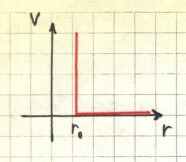
\includegraphics[scale=0.4]{images/1606337089.jpg}

Aquí $r_0$ es $\sigma$ y será la distancia mínima entre dos partículas. Este potencial ilustrado
es sencillamente
\[
	v(r) = \begin{cases}
		\infty \quad r < r_0 \\
		0      \quad r > r_0
	       \end{cases}
\]
Se tienen
\[
	a_2 = \frac{2\pi}{\lambda^3} \frac{r_0^3}{3}
\]
que lleva a $B_2 = 2 \pi r_0^3 / 3$. Se considera a las partículas como esferas duras (bolas de
radio $r_0/2$) entonces $B_2 = 4 v_0$ que conduce a 
\[
	\frac{Pv}{kT} = 1 + 4 v_0 f + ...
\]
y vemos que la $P_{ER} > P_{GI}$.

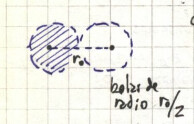
\includegraphics[scale=0.5]{images/1606337092.jpg}

DIBUJO 

\[
	b_2 = \frac{1}{2\lambda^3 V} \int_0^\infty du 4 \pi u^2 f_u = \frac{-1}{2\lambda^3 V} \frac{4\pi\sigma^3}{3}
\]

Sea ahora un potencial de Lenard-jones aproximado.

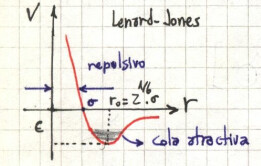
\includegraphics[scale=0.5]{images/1606337096.jpg}

Es algo como
\[
	V(r) =  4 \vare \left[ \Frac{ \sigma }{r}^12 - \Frac{ \sigma }{r}^6 \right]
\]
\[
	V(r) = \begin{cases}
		\infty \quad r < r_0 \\
		\\
		\displaystyle -U_0\Frac{r_0}{r}^b      \quad r > r_0
	       \end{cases}
\]
Entonces el coeficiente es
\[
	a_2 = \frac{2\pi}{\lambda^3} 
	\int_0^{r_0} \: r^2 \: dr + \int_{r_0}^\infty \: ( 1 - \euler^{u_0/(kT)(r_0/r)^b} ) r^2 \: dr 
\]
y aproximaremos van der Waals con $\mu_0/(kT) \ll 1$ (i.e. energía térmica mucho mayor que el pozo de potencial)
de manera que 
\[
	( 1 -  \euler^{u_0/(kT)(r_0/r)^b} ) \approx \frac{\mu_0}{kT} \Frac{r_0}{r}^b
\]
\[
	a_2(T) \approx  \frac{2\pi r_0^3}{\lambda^33} \left( 1 - \frac{u_0}{kT} \right)
\]
\[
	P = \frac{ N k T }{V} \left[ 1 + \frac{2\pi r_0^3}{v} \left( 1 - \frac{u_0}{kT} \right) \right]
	= \frac{ N k T }{V} \left( 1 - \frac{B_2}{v} \right) 
\]
Se puede ir a la ecuación de Van der Waals
\[
	 \left( P + \frac{2\pi r_0^3 u_0}{3v^2} \right) = \frac{kT}{v} \left( 1 + \frac{2\pi r_0^3}{3} \frac{1}{v} \right)
\]
donde en el último término dentro del paréntesis el primer factor es el volumen asociado con el {\it carozo duro}
del potencial y el segundo el volumen específico. Estamos usando la aproximación de gas diluido, es decir
que $ r_0 \ll v^{1/3}$.

Recordando la aproximación usual de $ (1+x)^u \sim 1 + u x $ se logra
\[
	\left( P + \frac{2\pi r_0^3 u_0}{3v^2} \right) \approx 
	\frac{kT}{v} \left( 1 - \frac{2\pi r_0^3}{3} \frac{1}{v} \right)^{-1}
\]
\[
	\left( P + \frac{a}{v^2} \right) (v - b) = k T
\]
de suerte que se tienen
\[
	a =(2/3) \pi r_0^3 u_0
	\qquad 
	b = 2 \pi /3 r_0^3
\]

Podemos relacionar los parámetros $a,b$ de Van der Waals con cosas microscópicas

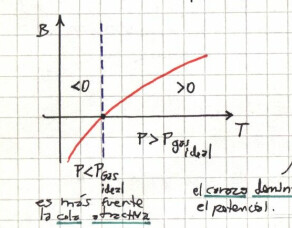
\includegraphics[scale=0.5]{images/1606337115.jpg}

Con este material los problemas 1,3,5,6 pueden encararse.
\notamargen{La flecha cortada en el gráfico este dice que ``partículas coon mucha
energía solo chocan''.}

Lo que sigue a continuación tal vez sea de esferas rígidas o tal vez sea de algo totalmente
diferente. No lo sé.

\[
	Z_3 = \int d^3q_1 \int d^3q_2 \int d^3q_3 \; ( 1 + f_{12} ) ( 1 + f_{13} ) ( 1 + f_{23} )
\]
\begin{multline*}
	Z_3 = 	\int d^3q_1 d^3q_2 d^3q_3 + \int d^3q_1 d^3q_2 d^3q_3 \: f_{12} +
	\int d^3q_1 d^3q_2 d^3q_3 \: f_{13} + \\ \int d^3q_1 d^3q_2 d^3q_3 \: f_{23} +
	\int d^3q_1 d^3q_2 d^3q_3 \: f_{12}f_{13}  + \int d^3q_1 d^3q_2 d^3q_3 \: f_{12}f_{23} + \\
	\int d^3q_1 d^3q_2 d^3q_3 \: f_{13}f_{23} + \int d^3q_1 d^3q_2 d^3q_3 \: f_{12}f_{13}f_{23} 
\end{multline*}
\[
	Z_3 = + + + + + + 
\]
(muchos dibujitos)

Se observa cierta degeneración. Podemos dar los números de ocupación de cada N-grafo
\[
\begin{aligned}
	\{ m_l \} = & (3,0,0) \qquad \text{ 1er N-grafo } \\
	\{ m_l \} = & (1,1,0) \qquad \text{ 2-4 N-grafo } \\
	\{ m_l \} = & (0,0,1) \qquad \text{ 5-8 N-grafo }
\end{aligned}
\]

Son sólo tres conjuntos $\{ m_l \}$ que describen todos los ocho 3-grafos. Sumamos los diferentes permutaciones de 
etiquetas distinguibles de cada conjunto $\{ m_l \}$
\[
	S((3,0,0)) = [  ]^3 = [\lambda^0 V b_1 ]^3
\]
\[
	S((1,1,0)) = []^1[]^1 = 3! [\lambda^0 V b_1 ]^1 [\lambda^3 V b_2 ]^1
\]
\[
	S((0,0,3)) = []^3 = 3! [\lambda^6 V b_3 ]^1
\]
\[
	\sum_{ \{ m_l \} } = 3! \left[ \frac{(V b_1)^3}{3!} + \lambda^3 V^2 b_1 b_2 + \lambda^6 V b_3 \right]
\]

\subsection{hoja suelta --reubicar--}
\[
	\hat{\rho} = \frac{\euler^{\beta \hat{H}}}{Q_N(V,T)} \quad \rightarrow \quad 
	\text{ Tr }(\hat{\rho}) = \frac{1}{Q_N(V,T)} \text{ Tr }(\euler^{\beta \hat{H}})
\]
\[
	1 =  \frac{1}{Q_N(V,T)} \text{ Tr }(\euler^{\beta \hat{H}})
\]
\[
	Q_N(V,T) = \text{ Tr }(\euler^{\beta \hat{H}})
\]

Pero la traza debe evaluarse en alguna base dada,
\[
	\text{ Tr }(\euler^{\beta \hat{H}}) = 
	\int \Bra{\vb{q}_1,..., \vb{q}_N} \euler^{-\beta \hat{H}} \Ket{\vb{q}_1,..., \vb{q}_N} d^{3N}q
\]
\[
	= \int \Bra{\vb{q}_1,..., \vb{q}_N} \euler^{-\beta \hat{H}} 
	\sum_E \Ket{\Psi_E} \braket{\Psi_E | \vb{q}_1,..., \vb{q}_N} d^{3N}q
\]
\[
	= \int  \sum_E \euler^{ -\beta E }  \braket{\vb{q}_1,..., \vb{q}_N | \Psi_E} 
	\braket{\Psi_E | \vb{q}_1,..., \vb{q}_N} d^{3N}q
\]
\[
	\text{ Tr }(\euler^{\beta \hat{H}}) = 
	\int \sum_E \euler^{ -\beta E }  \Psi_E (\vb{q}_1,..., \vb{q}_N ) 
	\Psi_E^*(\vb{q}_1,..., \vb{q}_N ) d^{3N}q
\]
donde $\Ket{\Psi_E}$ son autoestados de energía del $\hat{H}$. Usaremos la función de onda simetrizada y normalizada
\[
	\Psi_E (\vb{q}_1,..., \vb{q}_N )  =
\]
\begin{multline*}
	\Psi_E \Psi_E* = \frac{1}{N!} \sum_{\mathbb{P},\mathbb{P}'} \delta \mathbb{P} u_1(\mathbb{P}_1)
	u_2(\mathbb{P}_2) ... \delta \mathbb{P}' u(\mathbb{P}'_1)(1) u(\mathbb{P}'_2) (2) ... \\
	\sum_{\mathbb{P}} \delta(\mathbb{P}) u_1(\mathbb{P}_1) u_1^*(1) u_2(\mathbb{P}_2) u_2^*(2) ...
\end{multline*}


Una función de onda de $N$ partículas correctamente normalizada y simetrizada
\be
	\Psi (\vb{q}_1,..., \vb{q}_N ) = \frac{1}{\sqrt{N!}} \sum_{ \mathbb{P} } \delta \mathbb{P} \; \mathbb{P}
	\{ u_1(\vb{q}_1) u_2(\vb{q}_2) ... \}
	\label{fun_onda_norm}
\ee
\notamargen{$\mathbb{P}$ es el operador de permutaciones}
donde 
\[
	\Psi_B (\vb{q}_1,..., \vb{q}_N ) = \prod_{i=1}^{n_1} u_1(\vb{q}_1) \prod_{i=n_1+1}^{n_1+n_2} u_2(\vb{q}_2)
\]
es una función para partículas distinguibles (de Boltzmann).

Cada
\notamargen{Estas $\Psi$ son autofunciones del $\hat{H}$.}
\[
	u_{p_i}(\vb{q}_i) = \frac{1}{\sqrt{V}} \euler^{ i \vb{p}_i \cdot \vb{q}_i / \hbar }
\]
es función de onda de la partícula i-ésima en el ninvel energético $e_i$ dado por 
\[
	e_i = \frac{|\vb{p}_i|^2}{2m}
\]

Dado que sumamos en todas las permutaciones de \eqref{fun_onda_norm} es lo mismo permutar coordenadas que vectores
\[
	\Psi (\vb{q}_1,..., \vb{q}_N ) = \frac{1}{\sqrt{N!}} \sum_{ \mathbb{P} } \delta \mathbb{P} \;
	\left( u_{\mathbb{P}_1}(1) u_{\mathbb{P}_2}(2) ... \right) = 
	\frac{1}{\sqrt{N!}} \sum_{ \mathbb{P} } \delta \mathbb{P} \;
	\left( u_1({\mathbb{P}_1}) u_2({\mathbb{P}_2}) ... \right)
\]
\begin{multline*}
	\Psi (\vb{q}_1,..., \vb{q}_N ) \Psi^* (\vb{q}_1',..., \vb{q}_N' ) = \frac{1}{N!} \times \\
	\sum_{\mathbb{P}} \;  \delta \mathbb{P} \; \left(  u_1({\mathbb{P}_1}) u_2({\mathbb{P}_2}) ...\right)
	\sum_{\mathbb{P}'} \;  \delta \mathbb{P}' \; \left(  u_{\mathbb{P}_1}^*(1') u_{\mathbb{P}_2}^*(2') ... \right)\\
	= \frac{1}{N!} \sum_{\mathbb{P},\mathbb{P}'}\delta \mathbb{P} \delta \mathbb{P}'
	\left[ u_1({\mathbb{P}_1}) u_{\mathbb{P}_1}^*(1') u_2({\mathbb{P}_2}) u_{\mathbb{P}_2}^*(2') ... \right]
\end{multline*}

Dado que las permutaciones sólo difieren en el orden de los términos consideramos sólo una permutación repetida $N!$ 
veces, con lo cual 
\[
	\Psi (\vb{q}_1,..., \vb{q}_N ) \Psi^* (\vb{q}_1',..., \vb{q}_N' ) =
	\sum_{\mathbb{P}} \delta \mathbb{P} 
	\left[ u_1({\mathbb{P}_1}) u_{\mathbb{P}_1}^*(1') u_2({\mathbb{P}_2}) u_{\mathbb{P}_2}^*(2') ... \right]
\]
\[
	\Psi (\vb{q}_1,..., \vb{q}_N ) \Psi^* (\vb{q}_1',..., \vb{q}_N' ) =
	\sum_{\mathbb{P}} \delta \mathbb{P}
	\left[ \frac{\euler^{ i \vb{p}_1 \cdot ( \mathbb{P}\vb{q}_1 - \vb{q}_1' )/\hbar} }{V} \times 
	\frac{\euler^{ i \vb{p}_2 \cdot ( \mathbb{P}\vb{q}_2 - \vb{q}_2' )/\hbar}}{V} \times ... \right]
\]
\notamargen{
\[
	\delta \mathbb{P} = \begin{cases}
	                     1 \qquad \text{ bosones } \\
	                     \pm 1 \qquad \text{ fermiones}\\
	                     \text{ (perm par o impar) }
	                    \end{cases}
\]}

Ahora sea el sistema de las $N$ partículas con energía $E$, es decir 
\[
	E = \sum_i^N \; \frac{|\vb{p}_i|^2}{2m} =
	\frac{1}{2m} \left( |\vb{p}_1|^2 + |\vb{p}_2|^2 + ... + |\vb{p}_N|^2 \right)
\]
el estado energético será función de un vector $\vb{P}$
\[
	\vb{P} = (\vb{p}_1, \vb{p}_2, ..., \vb{p}_N )
\]
quiero evaluar 
\[
	\braket{ \{ \vb{q} \} | \euler^{\beta \hat{H}} | \{ \vb{q} \} } =
	\sum_P \euler^{-\beta E(P)} \Psi (\vb{q}_1,..., \vb{q}_N ) \Psi^* (\vb{q}_1',..., \vb{q}_N' )
\]
\notamargen{Suma en todos los $P$ posibles.}
pero esta sumatoria en $P$ es equivalente a 
\[
	\frac{1}{N!} \sum_{\vb{p}_1} \sum_{\vb{p}_2} ... \sum_{\vb{p}_N} 
	\euler^{-\beta/2m \left( |\vb{p}_1|^2 + |\vb{p}_2|^2 + ... + |\vb{p}_N|^2 \right)}
\]

\begin{multline*}
	= \frac{1}{N!} \sum_{\vb{p}_1} \sum_{\vb{p}_2} ... \sum_{\vb{p}_N} 
	\euler^{-\beta/2m \left( |\vb{p}_1|^2 + |\vb{p}_2|^2 + ... + |\vb{p}_N|^2 \right)} \times \\ 
	\sum_{ \mathbb{P} } \delta\mathbb{P} \: \frac{\euler^{ i \vb{p}_1 \cdot ( \mathbb{P}\vb{q}_1 - \vb{q}_1')/ 
	\hbar} }{V} \times \frac{\euler^{ i \vb{p}_2 \cdot ( \mathbb{P}\vb{q}_2 - \vb{q}_2' )/\hbar} }{V}\times ...
\end{multline*}
\[
	= \frac{1}{N!}\sum_{ \mathbb{P} } \delta\mathbb{P} \: \left( 
	\sum_{\vb{p}_1} \frac{\euler^{ -\beta/2m|\vb{p}_1|^2 + i \vb{p}_1 \cdot \vb{r}_1/ \hbar} }{V} \times 
	\sum_{\vb{p}_2} \frac{\euler^{ -\beta/2m|\vb{p}_2|^2 + i \vb{p}_2 \cdot \vb{r}_2/ \hbar} }{V} \times ...
	\right)
\]
donde 
\[
	\vb{r}_i = ( \mathbb{P}\vb{q}_i - \vb{q}_i')
\]

La cuenta entre paréntesis es integrable pasando al continuo con 
\[
	\frac{V}{h^3} \delta \vb{p}_i = 1 \quad \rightarrow \quad \frac{d\vb{p}_i}{h^3} = \frac{1}{V}
\]
\[
	= \frac{1}{N!} \sum_{ \mathbb{P} } \delta\mathbb{P} \: \left( 
	\frac{1}{h^3} \int d\vb{p}_1 \euler^{ -\beta/2m|\vb{p}_1|^2 + i \vb{p}_1 \cdot \vb{r}_1/ \hbar} \times 
	\frac{1}{h^3} \int d\vb{p}_2 \euler^{ -\beta/2m|\vb{p}_2|^2 + i \vb{p}_2 \cdot \vb{r}_2/ \hbar} \times ...
	\right)
\]

Descomponemos cada integral en tres
\[
	I \equiv \left[ \frac{1}{h} \int dp_x \euler^{ -\beta/2m p_x^2 + i p_x r_x/ \hbar} \right] 
	\left[ \frac{1}{h} \int dp_y ... \right] \left[ \frac{1}{h} \int dp_z ... \right]
\]

Usamos que 
\[
	\int dp \euler^{-ap^2} \euler^{-ibp} = \frac{\sqrt{\pi}}{\sqrt{a}} \euler^{-b^2/(4a)}
\]
\[
	I_x = \frac{1}{h} \sqrt{\frac{2\pi m}{\beta}} \euler^{-\frac{2r^2m}{4\beta \hbar^2}} =
	\frac{1}{h} \sqrt{2\pi m kT} \euler^{-\frac{2mkT\pi^2 r^2}{h^2}} = 
	\frac{1}{\lambda} \euler^{-r_x^2\pi /\lambda^2}
\]
\[
	I = I_x I_y I_z = \frac{1}{\lambda^3} \euler^{ -\frac{\pi}{\lambda^2}
	[ (\mathbb{P}q_x-q_x')^2 + (\mathbb{P}q_y-q_y')^2 + (\mathbb{P}q_z-q_z')^2 ]} = 
	\frac{1}{\lambda^3} \euler^{ -\frac{\pi}{\lambda^2} |\vb{r}|^2 }
\]

Luego,
\[
	= \frac{1}{N!} \sum_{ \mathbb{P} } \delta\mathbb{P} \frac{1}{\lambda^{3N}}
	\euler^{ -\frac{\pi}{\lambda^2} |\vb{r}_1|^2 } \times \euler^{ -\frac{\pi}{\lambda^2} |\vb{r}_2|^2 } \times ...
\]

Definimos
\[
	f( \vb{r}_i ) = \euler^{ -\frac{ \pi |\vb{r}_i|^2 }{ \lambda^2 } } \qquad 
	f( \mathbb{P}\vb{q}_i - \vb{q}_i' ) = \euler^{ -\frac{ \pi }{ \lambda^2 }(\mathbb{P}\vb{q}_i - \vb{q}_i')^2 }
\]

Resultando 
\[
	= \frac{1}{N!\lambda^{3N}} \sum_{\mathbb{P}} \delta\mathbb{P} [ f( \mathbb{P}\vb{q}_1 - \vb{q}_1' ) ... 
	f( \mathbb{P}\vb{q}_N - \vb{q}_N' )]
\]
\[
	\braket{ \vb{q}_1,..., \vb{q}_N|\euler^{-\beta\hat{H}}| \vb{q}_1',..., \vb{q}_N' } = 
	\frac{1}{N!\lambda^{3N}} \sum_{\mathbb{P}} \delta\mathbb{P} [ f( \mathbb{P}\vb{q}_1 - \vb{q}_1' ) \times 
	... \times f( \mathbb{P}\vb{q}_N - \vb{q}_N' )]
\]
\begin{multline*}
	\text{ Tr} (\euler^{-\beta\hat{H}}) = \int d^{3N} q
	\braket{ \vb{q}_1,..., \vb{q}_N|\euler^{-\beta\hat{H}}| \vb{q}_1',..., \vb{q}_N' } =\\
	\frac{1}{N!\lambda^{3N}} \int d^{3N}q \sum_{\mathbb{P}} \delta\mathbb{P} [ f( \mathbb{P}\vb{q}_1 - \vb{q}_1' ) 
	\times ... \times f( \mathbb{P}\vb{q}_N - \vb{q}_N' )]
\end{multline*}
\[
	\text{ Tr} (\euler^{-\beta\hat{H}}) = \frac{1}{N!\lambda^{3N}} \int d^{3N}q \sum_{\mathbb{P}} 
	\delta\mathbb{P} \prod_i f( \mathbb{P}\vb{q}_i - \vb{q}_i )
\]

Analizamos la $\sum_{\mathbb{P}}$. Como se suma en todas las permutaciones, tendremos
\[
	\sum_{\mathbb{P}} f(\mathbb{P}{q}_1 - {q}_1) f(\mathbb{P}{q}_2 - {q}_2) ... =
\]
\[
	1 \: f(0) \pm \sum_{i<j} f_{ij} f_{ji} + \sum_{i<j<k} f_{ij} f_{jk} f_{ki} \pm ...
\]
\[
	\text{ 0 permut } \qquad \text{ 1 permut } \qquad \text{ 2 permut }
\]

Veamos la permutación de $q_1$ y $q_2$
\[
	\underbrace{\mathbb{P}}_{=1} (\prod_i f( \mathbb{P}\vb{q}_i - \vb{q}_i ) ) =
	\underbrace{f(\mathbb{P}{q}_1 - {q}_1) f(\mathbb{P}{q}_2 - {q}_2)}_{f_{ij}f_{ji}}
	\underbrace{\prod_{i=3}^N f(q_i - q_i)}_{\prod f(0)=1}
\]
\[
	q_1 \; q_2 \; q_3 \; ... \; q_N
\]
\[
	q_1 \; q_2 \; q_3 \; ... \; q_N
\]

\[
	\underbrace{\mathbb{P}}_{=2} (\prod_i f( \mathbb{P}\vb{q}_i - \vb{q}_i ) ) =
	\underbrace{f( {q}_2 - {q}_1 )}_{f_{ij}} \underbrace{f( {q}_3 - {q}_2 )}_{f_{ki}}
	\underbrace{f( {q}_1 - {q}_3 )}_{f_{jk}}
	\prod_{i=4}^N f(0)
\]
\[
	q_1 \; q_2 \; q_3 \; ... \; q_N
\]
\[
	q_1 \; q_2 \; q_3 \; ... \; q_N
\]

\[
	\underbrace{\mathbb{P}}_{=3} (\prod_i f( \mathbb{P}\vb{q}_i - \vb{q}_i ) ) =
	f( {q}_2 - {q}_1 ) f( {q}_1 - {q}_2 ) f( {q}_4 - {q}_3 ) f( {q}_3 - {q}_4 ) 
	\prod_{i=5}^N f(0)
\]
\[
	q_1 \; q_2 \; q_3 \; q_4 \; ... \; q_N
\]
\[
	q_1 \; q_2 \; q_3 \; q_4 \; ... \; q_N
\]
\[
	\text{ Tr} (\euler^{-\beta\hat{H}}) = \frac{1}{N!\lambda^{3N}} \int d^{3}q 
	\left( 1 \pm \sum_{i<j} f_{ij} f_{ji}  \right)
\]
\notamargen{El $+$ es por bosones y el $-$ por fermiones.}
\[
	f_{ij} = \euler^{ -\frac{\pi}{\lambda^2} |\vb{q}_i - \vb{q}_j|^2} =
	\euler^{ -\frac{\pi}{h} 2\pi k T |\vb{q}_i - \vb{q}_j|^2}
\]

Veamos los límites clásico y el surgimiento de fenómenos cuánticos 
\[
	\text{ CLÁSICO } \qquad v = \frac{V}{N} \ggg 1 \quad \Rightarrow \quad 
	|\vb{q}_i - \vb{q}_j| \gg 1 \qquad T \ggg 1
\]
y por lo tanto
\[
	\euler^{ -\frac{\pi}{h} 2\pi k T |\vb{q}_i - \vb{q}_j|^2} \to 0
\]
\[
	\text{ Tr} (\euler^{-\beta\hat{H}}) = \frac{1}{N!\lambda^{3N}} \int d^{3}q (1) =
	\frac{1}{N!}\Frac{V}{\lambda^3}^N
\]
\[
	\Or(v) \approx 1 \quad \Rightarrow \quad \Or(|\vb{q}_i - \vb{q}_j|) \approx 1 \qquad
	\Or(T) \approx 1
\]
y en este caso es
\[
	\euler^{ -\frac{\pi}{h} 2\pi k T |\vb{q}_i - \vb{q}_j|^2} \to 1
\]
\begin{multline*}
	\text{ Tr} (\euler^{-\beta\hat{H}}) \cong \frac{1}{N!\lambda^{3N}} \int d^{3}q 
	\left( 1 \pm \sum_{i<j} f_{ij} f_{ji}  \right) \\ 
	\cong \frac{1}{N!\lambda^{3N}} \int d^{3}q 
	\left[ \prod_{i<j} (1 \pm f_{ij} f_{ji} ) \right] 
\end{multline*}
\notamargen{Este pasaje vale si $f_{ij} f_{ji}$ es pequeño.}

\begin{multline*}
	\prod_{i<j} ( 1 \pm f_{ij}f_{ji}) = \displaystyle \euler^{\log \prod_{i<j} ( 1 \pm f_{ij}f_{ji}) } =
	\euler^{\displaystyle \sum_{i<j} \log ( 1 \pm f_{ij}f_{ji}) } = \\
	\euler^{\displaystyle -\beta \sum_{i<j}  kT \log ( 1 \pm f_{ij}f_{ji}) } =
	\euler^{\displaystyle -\beta \sum_{i<j}  V_{ij}^{\pm} }
\end{multline*}
donde 
\[
	V_{ij}^{\pm} = -kT\log \left( 1 \pm \euler^{-\frac{\pi}{\lambda^2}|\vb{q}_i - \vb{q}_j|^2} 
	\euler^{-\frac{\pi}{\lambda^2}|\vb{q}_j - \vb{q}_i|^2} \right) =
	-kT\log \left( 1 \pm  \euler^{-2\frac{\pi}{\lambda^2}|\vb{q}_i - \vb{q}_j|^2} \right)
\]

Con $ | \vb{q}_i - \vb{q}_j| \to 0 $ es
\[
	V_{ij}^{\pm} = -kT\log ( 1 \pm 1 ) = \begin{cases}
	                                           -kT\log (2) \quad \text{ bosones } \\
	                                           -kT\log (o^+) \quad \text{ fermiones } 
	                                          \end{cases}
\]

DIBUJO 

El potencial efectivo $\beta V_{ij}$ luce como la Figura


Límite clásico $\to$ no permutación 

Cuando hay overlap de las funciones de onda de las partículas hay que realizar las permutaciones correspondientes.

La simetría (por la indistinguibilidad que hace necesaria la permutación) lleva a términos efectivos de interacción 
repulsivos (FD) o a atractivos (BE).

\subsection{Parte de gases reales (desde carpeta)}

En el límite clásica la $Z$ se factoriza.
Eso explica los apartamientos del comportamiento Boltzmann. El gas ideal cuántico no tiene correlación dinámica,
sino solo las asociadas al carácter de simetría de la función de onda.

\notamargen{En la carpeta estaba la observación de que: ``salteamos la clase de cuánticos 6''}.


\subsection{Otra cosa suelta --reubicar--}

El parámetro de comportamiento siempre es
\[
	\frac{\lambda^3}{v} = \frac{h^3/(2\pi m kT)^{3/2}}{V/N}
\]
donde la longitud de onda térmica $\lambda = h/(2\pi m kT)^{1/2}$ es una medida que da idea de la dispersión de la 
partícula de masa $m$ y temperatura $T$ considerada como onda. El volumen específico $v=V/N$ es el volumen promedio 
ocupado por una partícula. Luego, $\lambda^3$ es una especie de volumen de la partícula considerada como onda.
Si 
\[
	\lambda^3 > v \qquad \text{ Fenómenos de interferencia cuántica }
\]
\[
	\lambda^3 < v \qquad \text{ No hay fenómenos de interferencia cuántica }
\]

GRAFIQUETES

$\lambda$ es una característica del sistema de partículas $(m,T)$
\begin{center}
\begin{tabular}{c c}
$\displaystyle \frac{\lambda^3}{v} \ggg 1 $ & $\displaystyle \frac{\lambda^3}{v} \lll 1 $ \\
Altamente cuántico &  Altamente clásico\\
alta $N/V$ & baja $N/V$\\
baja T & alta T
\end{tabular}
\end{center}

Para Bose el análisis parte de 
\[
	\euler^{-\beta(e-\mu)} < 1 \quad \rightarrow \quad \mu < e \to \mu < 0
\]
\notamargen{gas ideal $e_0=0$, todas con $\vb{p}=0$}
para toda $e$ del sistema, lo cual hará que 
\[
	0 < z < 1 
\]
y
\[
	\frac{N}{V} = \frac{1}{\lambda^3} g_{3/2}(z) + \frac{1}{V} \frac{z}{1-z}
\]

Como $z$ es a lo sumo 1, entonces $g_{3/2}(z)$ está acotada y $g_{3/2}(1)=2.612$
\[
	\frac{\lambda^3}{v} = g_{3/2}(z) + \frac{\lambda^3}{V} \Frac{z}{1-z}
\]

Cuando $z=1$, $g_{3/2}$  ya no puede crecer más; si sube $N$ el remanente $(N-N_e)$ va al estado 
$e_0=0$
\[
	\frac{\lambda^3}{v}(N_e+N_0) = \underbrace{g_{3/2}(z)}_{\lambda^3/V N_e} + \frac{\lambda^3}{V} N_0
\]

Definimos $T_c, v_c$ a partir de $\frac{\lambda^3}{v} = g_{3/2}(1)$ 

Si $ T<T_c$ o $v<v_c$ se tiene 
\[
	\frac{\lambda^3}{v} > g_{3/2}(1) \quad \Rightarrow \quad \frac{\lambda^3}{v} =
	g_{3/2}(1) + \frac{\lambda^3}{V} N_0
\]

Entonces tendremos 
\[
	z = 1 \quad \Rightarrow \quad \mu(T_c) = 0 \quad \Rightarrow \quad T=T_c \quad \Rightarrow \quad  
	\frac{\lambda^3}{v} = 2.612
\]
\[
	T < T_c \quad \Rightarrow \quad \mu(T) = 0 \quad \Rightarrow \quad z = 1 \quad \Rightarrow \quad  
	\frac{\lambda^3}{v} > 2.612
\]
\[
	T > T_c \quad \Rightarrow \quad \mu(T) < 0 \quad \Rightarrow \quad z < 1 \quad \Rightarrow \quad  
	\frac{\lambda^3}{v} < 2.612
\]
\[
	T \gg T_c \quad \Rightarrow \quad \mu(T) \ll 0 \quad \Rightarrow \quad z \ll 1 \quad \Rightarrow \quad  
	\frac{\lambda^3}{v} \ll 1
\]

El $\mu(T)$ luego del condensado $(T<T_c)$ se hace cero con lo cual $z=1$ para todo el intervalo.

Una vez que se tiene el condensado

GRAFICO

\subsection{Cuánticos 6}

comentario estadísticas

modelado de un metal

red de átomos -> gas de fonones -> $c_v$ fonones

Modelos de Debye -> distribución de $\omega$
Einstein -> $\omega = \omega_E$

Modelado de un metal (gas de electrones) -> $c_v$ electrónico

Emisión termoiónica

Tema pequeñas oscilaciones (leer mi resumen)
ver tema de ondas de sonido en sólidos.


%=================================================================================================
\section{Sistemas de partículas indistinguibles y no interactuantes}
% =================================================================================================

\begin{itemize}
 \item no interacción
 \item indistinguibilidad (partículas idénticas)
\end{itemize}

\[
	\hat{H} = \sum_i^N H_i (\vec{q}_i , \vec{p}_i )
\]
\[
	\hat{H} \Psi_E = E \Psi_E \qquad \text{ donde }
\]
\[
	\Psi_E = \prod_{i=1}^{N} u_{e_1}(q_i) \qquad \text{ y } u_{e_1}(q_i)
\]
siendo esta última la solución de una única partícula en el nivel $e_i$ 
y donde $e_i$ es el nivel energético de la partícula 'i'.

El sistema cuántico se describe mediante números de ocupación
\[
	E = \sum_{j=1}^L e_j n_j  \qquad \qquad  N = \sum_{j=1}^L  n_j
\]
siendo $n_j$ el número de partículas en el nivel de energía $e_j$ 
\[
	\Psi_E = \prod_{i=1}^{n_1} u_{e_1}(q_i) \cdot \prod_{i = n_1 + 1 }^{ n_1 + n_2 } u_{e_2}(q_i) \cdot ...
\]

Permutando coordenadas $(\vb{q}_1,\vb{q}_2,...,\vb{q}_N ) \to (P\vb{q}_1,P\vb{q}_2,...,P\vb{q}_N)$ llego a
\[
	\frac{N!}{n_1!n_2!...} = N! \prod_{i=1}^N \frac{1}{n_i!}
\]
diferentes estados. Cada vez que permuto dos partículas en diferentes niveles energéticos cuento un estado extra.

Podemos construir una función de onda cuántica correcta (que no se altere por permutaciones) si respetamos
\[
	| P\Psi |^2 = | \Psi |^2 \quad \text{ dos casos }
\]
\[
	P\Psi = \Psi \qquad \qquad \qquad P\Psi = 
	\begin{cases}
	+ \Psi \text{ número par de permutaciones } \\ 
	- \Psi \text{ número impar de permutaciones } 
	\end{cases}
\]
\[
	\text{ simétrica } \qquad \qquad \qquad \qquad \text{ antisimétrica } 
\]
\[
	\Psi = \sum_P P\Psi \qquad \qquad \qquad \Psi = \sum_P \delta_P P\Psi, \delta_P = \pm 1
\]
\notamargen{Faltaría el coeficiente de normalización}

La antisimetría puede escribirse como determinante de Slater. Además, una función antisimétrica $\Psi$ será nula 
al sumar en 'P' si existe más de una partícula en un mismo nivel energético. Esto equivale a tener dos filas
iguales en el determinante de Slater.
Vemos que el hecho de forzar la simetría de intercambio ha llevado al PRINCIPIO DE EXCLUSIÓN.

\begin{center}
\begin{tabular}{|l|l|l|}
\hline
 & & \\
BOSE-EINSTEIN & $ n_i = 0,1,2, ... , N $ & Cualquier ocupación es válida \\
 (spin entero) & & \\
FERMI-DIRAC  & $ n_i = o, 1 $ & Sólo puede haber a lo sumo una partícula por nivel \\
 (spin semientero) & & \\
\hline
\end{tabular}
\end{center}
\notamargen{La exclusión es $\sum_i^L n_i^2 = N$}

Entonces, dado un conjunto $ \{ n_i \} $ de números de ocupación tendré 

\begin{itemize}
\item 1 estado bosónico : $ \quad \Psi_S = \sum_P P \Psi_{\text{Boltz}}$
\item 1 estado fermiónico : $ \quad \Psi_A = \sum_P \delta_P P \Psi_{\text{Boltz}} 
	\; (\text{ si } N 0 \sum_i^N n_i^2 )$
\item $ \frac{N!}{\prod_i^L n_i!} $ estados de Boltzmann $ \Psi_{\text{Boltz}} = \prod_{i=1}^N u_i(\vec{q}_i) $
\end{itemize}


\subsection{Gas ideal cuántico}

Consideramos $N$ partículas no interactuantes indistinguibles ocupando un volumen $V$ y con energía $E$
Un estado es un conjunto $ \{ n_i^\nu \} $ donde 'i' es nivel energético
\be
	E_\nu = \sum_i e_i n_i^\nu \qquad \qquad N_\nu = \sum_i n_i^\nu
	\label{cond_EN}
\ee

En el microcanónico $ E_\nu = E $ y $ N_\nu = N $ para todo estado $\nu$. Pensamos en cierta estructura 
fina de niveles


donde $g_i$ es el número de subniveles energéticos en la celda 'i' y $n_i$ es el correspondiente número de
partículas en la celda 'i'.

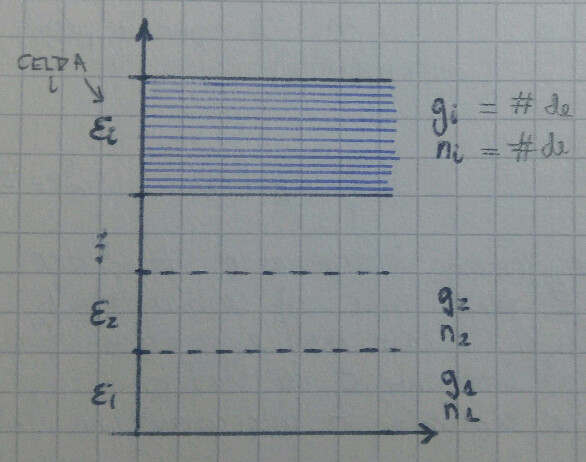
\includegraphics[scale=0.35]{images/1625623752.jpg}

Luego

\[
	\Gamma = \sum_{ \{ n_i \} }' W(\{ n_i \}) = \sum_{ \{ n_i \} }' \prod_i^L  \omega_i 
\]
tendremos
\begin{itemize}
 \item bosones $ \omega_i = \frac{ ( g_i - 1 + n_i)! }{ (g_i - 1)!n_i!} $
 \item fermiones $ \omega_i = \frac{ ( g_i - n_i + n_i )! }{ (g_i - n_i)!n_i!} =
		\frac{ g_i! }{ (g_i -n_i )! n_i!}$
 \item boltzmanniones $ \omega_i = g_i^{n_i} $ y hay que multiplicar por el factor
		$ N! / \prod n_i! $
\end{itemize}
donde $ \omega_i $ es el número de maneras de tener $ n_i $ en $ g_i $ subniveles.
\notamargen{Permutaciones de partículas y paredes (bosones). Permutaciones de partículas y huecos
$g_i \geq n_i $.}

Para el caso de Boltzmann debemos multiplicar por el factor de buen conteo,
\[
	\Gamma = \frac{1}{N!} \sum_{ \{ n_i \} }' \prod_i^L \frac{N!}{\prod (n_i)!}(g_i)^{n_i}
	= \sum_{ \{ n_i \} } \prod_i^L \frac{ (g_i)^{n_i} }{ (n_i)! }
\]

La entropía $S$ es
\[
	S = k \log \sum_{ \{ n_i \} }' W ( \{ n_i \} ) \approx k \log W( \hat{n}_i )
\]
donde se supone que el conjunto $ \{ \bar{n}_i \}$ domina la $ \sum' $. Buscaremos ese conjunto
extremando $S$ sujeto a las condiciones \eqref{cond_EN}.

\[
	\delta ( k\log W( \{ n_i \} ) ) + \alpha \delta N + \beta \delta E = 0
\]
\[
	\bar{n}_i = \frac{ g_i }{ \euler^{ -\beta \mu } \euler^{ \beta e_i } - 1 } \text{ Bose }
\]
\notamargen{Los coeficientes son para las dimensiones. Luego se ve que 
$ \alpha = -\mu / kT \quad \beta = 1 / kT \quad z \equiv \euler^{ \beta \mu} $}
\[
	\bar{n}_i = \frac{ g_i }{ \euler^{ -\beta \mu } \euler^{ \beta e_i } + 1 } \text{ Fermi }
\]
\[
	\bar{n}_i =  g_i \euler^{ \beta \mu } \euler^{ \beta e_i } \text{ Boltzmann }
\]

Esto da el número de partículas por celda energética 'e$_i$' pero interesará por nivel 'g$_i$'.
Entonces dividiremos sobre 'g$_i$' y cambiamos el índice 
\[
	n_j = \frac{1}{z^{-1}\euler^{\beta e_j} + a} \qquad 
	a = \begin{cases}
	 1 \text{ Bose } \\
	 -1 \text{ Fermi } \\
	 0 \text{ Boltmann }
	\end{cases}
\]

La identificación de los coeficientes puede hacerse desde 
\[
	U = TS - pV + \mu N \qquad TS = U  + pV - \mu N
\]
\[
	\frac{S}{k} = \frac{E}{kT} + \frac{pV}{kT} - \frac{\mu}{kT}N \qquad 
	\quad (S=S(E,V,N))
\]
\be
	\frac{S}{k} = \frac{1}{kT} \sum_i n_i e_i + \frac{pV}{kT} - \frac{\mu}{kT} \sum_i n_i
	\label{entropiaSoverk}
\ee

La idea es escribir $ S / k $ en \eqref{entropiaSoverk} de modo que queden explícitas las
$\sum$ que definen $N$ y $E$. Para Bose es 
\[
	\frac{S}{k} = \sum_i n_i \log \left( 1 + \frac{g_i}{n_i} \right) + 
	g_i \log \left( 1 + \frac{n_i}{g_i} \right)
\]
\[
	n_i \log ( n_i + g_i ) - n_i \log ( n_i ) = 
	n_i \log ( n_i \euler^{A} \euler^{Be_i} ) - n_i \log ( n_i )
\]
\[
	\sum_i n_i (A + Be_i) + g_i
\]
\[
	\frac{S}{k} = A \sum_i n_i + B \sum_i e_i n_i + \sum_i g_i \log \left( 1 + \frac{n_i}{g_i} \right)
\]
\[
	A = - \frac{ \mu }{ k T } \qquad \qquad B = \frac{1}{ kT }
\]

\subsection{Microcanónico cuántico (gas ideal) de Boltzmann}

Se puede hacer la cuenta explícitamente.
\[
	\frac{S}{k} = \log \left( \prod_i \frac{}{} \right) =
	\sum_i n_i \log (g_i) - \log n_i!
\]
\[
	\frac{S}{k} \approx 	\sum_i n_i \log \left(\frac{g_i}{n_i}\right) + n_i =
	\sum_i n_i \left( \log (g_i/n_i) + 1 \right)
\]
\[
	N = \sum_i g_i z \euler^{-\beta e_i} = \sum_j z\euler^{-\beta e_j} =
	\frac{1}{h^3} \int d^3p z \euler^{-\beta p^2 / 2m } \int d^3 q =
	\frac{zV}{h^3} (2\pi m k T)^{3/2} = \frac{zV}{\lambda^3}
\]
donde hemos preparado el paso al continuo

En Boltmann es 
\[
	N = \frac{zV}{\lambda^3} \quad \rightarrow \quad z = \frac{\lambda^3}{v} \ll 1 
\]
\[
	E = \frac{3}{2}NkT \qquad \frac{S}{k} = \beta E - N \log( z ) + N
\]


% =================================================================================================
\section{Cuánticos II}
% =================================================================================================

\begin{itemize}
 \item Gas ideal en el gran canónico, entonces el cálculo de $Q_N$ previamente
 \item Gas ideal (Boltmann) en el canónico $\to$ multinomial
\[
	Q_N = \frac{1}{N!} \sum_{n_1}' \sum_{n_2}' ...  \sum_{n_i}' \frac{N!}{n_1!n_2!...}
	\euler^{ -\beta \sum_i n_i e_i }
\]
\[
	Q_N = \frac{1}{N!} \sum_{n_1}' \sum_{n_2}' ...  \sum_{n_i}' \frac{N!}{n_1!n_2!...}
	\prod_i^L \euler^{ -\beta n_i e_i }
\]
\[
	Q_N = \frac{1}{N!} \left( \euler^{-\beta e_1 } + \euler^{ -\beta e_2 } + ... \right)^N
	= \frac{1}{N!} \left( \sum_i \euler^{-\beta e_i } \right)^N =
	\frac{1}{N!} \left( \frac{V}{\lambda^3} \right)^N 
\]
\[
	\log (Q_N) = N \log ( V/\lambda^3 ) - N \log N + 1
\]
\[
	\frac{1}{N} \approx \log \left( \frac{v}{\lambda^3} \right)
\]
\[
	\boxed{ \log Q_N = N \left[ \log \left( \frac{v}{\lambda^3} \right) + 1 \right]}
\]
\item Gas ideal (Fermi y Bose) en el canónico $\to$ {\it hard} $\to$ paso al gran canónico.
\[
	\Xi = \sum_{n=0}^\infty z^N Q_N(V,T)
\]
\[
	\Xi = \sum_{n=0}^\infty \euler^{\beta \mu N} \sum_{n_1}' \sum_{n_2}' ...  \sum_{n_i}' 
	\euler^{ -\beta \sum_i n_i e_i }
\]
y con un {\it magic pass}
\[
	\Xi =  \sum_{n_1}^\infty \sum_{n_2}^\infty ... \sum_{n_i}^\infty
	\euler^{ \beta \mu \sum_i n_i } \euler^{ -\beta \sum_i n_i e_i }
	= \sum_{n_1}^\infty \sum_{n_2}^\infty  ... \sum_{n_i}^\infty \prod_i \euler^{\beta(\mu -e_i )n_i}
\]
\[
	\Xi =  \prod_i^L \left( \sum_{n_i=0}^\infty \euler^{\beta(\mu -e_i )n_i} \right)
\]

Para Boltzmann el gran canónico será 
\[
	\Xi = \sum_{N=0}^\infty \frac{1}{N!} \left( \frac{zV}{\lambda^3}\right)^N
\]
\[
	\Xi(z,V,T) = \begin{cases}
	              \prod_i \frac{1}{1- \euler^{\beta(\mu - e_i)}} \qquad \text{ Bose } \\
	              \prod_i 1 + \euler^{\beta(\mu - e_i)} \qquad \text{ Fermi } \\
	              \euler^{zV/\lambda^3} \qquad \text{ Boltzmann }
	             \end{cases}
\]
\[
	\log \Xi(z,V,T) = \frac{pV}{kT} = \begin{cases}
	              \sum_i -\log (1 - \euler^{\beta(\mu - e_i)} ) \qquad \text{ Bose } \\
	              \sum_i \log (1 + \euler^{\beta(\mu - e_i)} )  \qquad \text{ Fermi } \\
	              \frac{zV}{\lambda^3} = z\sum_i^L \euler^{-\beta e_i} \qquad \text{ Boltzmann }
	             \end{cases}
\]

El número de partículas sale desde 
\[
	\braket{N} = z\dpar{}{z} ( \log \Xi(z,V,T) )
\]
\[
	\braket{N} = \begin{cases}
	             z \sum_i -\frac{1}{1-z\euler^{-\beta e_i}} (-\euler^{-\beta e_i}) =
	             \sum_i \frac{1}{ z^{-1}\euler^{\beta e_i} - 1 } \qquad \text{ Bose } \\
	             z \sum_i \frac{1}{1+z\euler^{-\beta e_i}} (\euler^{-\beta e_i}) =
	             \sum_i \frac{1}{ z^{-1}\euler^{\beta e_i} + 1 } \qquad  \text{ Fermi } \\
	             \frac{zV}{\lambda^3} \qquad \qquad \text{ Boltzmann }
	             \end{cases}
\]
\[
	\braket{n_j} = -\dpar{}{\beta e_j} ( \log \Xi(z,V,T) )
\]
\[ 
	\braket{n_j} = \begin{cases}
	 \displaystyle   -\frac{-1}{1-z\euler^{-\beta e_i}} (-z\euler^{-\beta e_i})(-1) =
			\frac{1}{ z^{-1}\euler^{\beta e_i} - 1 } \qquad \text{ Bose } \\
			\\
	 \displaystyle    \frac{-1}{1+z\euler^{-\beta e_i}} (z\euler^{-\beta e_i})(-1) =
	             \frac{1}{ z^{-1}\euler^{\beta e_i} + 1 } \qquad  \text{ Fermi } \\
	             \\
	 \displaystyle  z \euler^{-\beta e_j} \qquad \qquad \qquad \qquad \qquad \qquad \text{ Boltzmann }
	             \end{cases}
\]
\end{itemize}


\subsection{Funciones termodinámicas}

Todo comienza desde la función de partición

\begin{center}
\begin{tabular}{c|c}
 Fermi &  Bose \\
  & \\
$ \displaystyle \Xi = \prod_i 1 + \euler^{-\beta(e_i - \mu)} $ & 
$ \displaystyle \Xi = \prod_i \frac{1}{1 - \euler^{-\beta(e_i - \mu)}} $ \\
  & \\
$ \displaystyle \beta p V = \sum_i \log (1 + \euler^{-\beta(e_i - \mu)}) $  & 
$ \displaystyle \beta p V = \sum_i -\log (1 - \euler^{-\beta(e_i - \mu)}) $ \\
 & 
\end{tabular}
\end{center}

En gas ideal es, en cartesianas, 
\[
	e = \frac{|\vec{p}|^2}{2m} = ( p_x^2 + p_y^2 + p_z^2 )/2m 
\]
o en esféricas
\[
	e = \frac{p^2}{2m} 
\]

Un gas ideal cuántico generalizará al gas ideal clásico y para valores determinados de los
parámetros ($T,V$ grandes) debería devolver el resultado clásico.
\begin{center}
\begin{tabular}{c|c}
  & \\
$ \displaystyle \braket{N} = \sum_i \frac{1}{\euler^{\beta(e_i - \mu)} + 1} $ & 
$ \displaystyle \braket{N} = \sum_i \frac{1}{\euler^{\beta(e_i - \mu)} - 1} $ \\
  & 
\end{tabular}
\end{center}

El paso al continuo y la integración por partes luego del reemplazo
\[
	\beta e = \frac{\beta p^2}{2m} = \frac{p^2}{2mkT} \cong x
\]
llevará a 
\begin{center}
\begin{tabular}{c|c}
$ \displaystyle \beta p = \frac{1}{\lambda^3} f_{5/2}(z) $ & 
$ \displaystyle \beta p = \frac{1}{\lambda^3} g_{5/2}(z) $ \\
  & \\
$ \displaystyle \frac{\braket{N}}{V} = \frac{1}{\lambda^3} f_{3/2}(z) $ & 
$ \displaystyle \frac{\braket{N}}{V} - \frac{N_0}{V}= \frac{1}{\lambda^3} g_{3/2}(z) $ \\
  & 
\end{tabular}
\end{center}


\notamargen{$ n_0 = \frac{1}{z^{-1} - 1 } = \frac{z}{1-z}$ se va a $\infty$ con 
$z\to 1$ que es $\mu \to 0$.}
Así queda todo en función de 
\[
	f_\nu(z) = \frac{1}{\Gamma(\nu)} \int_0^\infty \frac{x^{\nu-1}}{z^{-1}\euler^x + 1} dx \qquad \text{ y }
	g_\nu(z) = \frac{1}{\Gamma(\nu)} \int_0^\infty \frac{x^{\nu-1}}{z^{-1}\euler^x - 1} dx
\]
\begin{center}
\begin{tabular}{c|c}
  & \\
$ \displaystyle \frac{\lambda^3}{v} = f_{3/2}(z) $ & 
$ \displaystyle \frac{\lambda^3}{v}( N - n_0 ) = g_{3/2}(z) $ \\
  & 
\end{tabular}
\end{center}
\notamargen{$N-n_0$ es la población en los estados excitados.}

Pero tenemos expresiones en términos de $z$
\begin{center}
\begin{tabular}{c|c}
  & \\
$ \displaystyle f_\nu (z) = \sum_{j=1}^\infty \frac{(-1)^{j+1}z^j}{j^\nu} $ & 
$ \displaystyle g_\nu (z) = \sum_{j=1}^\infty \frac{z^j}{j^\nu}  $ \\
  & 
\end{tabular}
\end{center}

Podemos escribir
\begin{center}
\begin{tabular}{c|c}
  & \\
$ \displaystyle \frac{\lambda^3}{v} = z - \frac{z^2}{2^{3/2}} + \frac{z^3}{3^{3/2}}  - ... \qquad $ & 
$ \displaystyle \frac{\lambda^3}{v}( N - n_0 ) = z + \frac{z^2}{2^{3/2}} + \frac{z^3}{3^{3/2}}  - ... \qquad $ \\
  & 
\end{tabular}
\end{center}
con lo cual con $z \ll 1$ nos podemos quedar con los primeros términos.
Asimismo $ n_0 \ll N$.
\begin{center}
\begin{tabular}{c|c}
  & \\
$ \displaystyle \beta p = \frac{z - \frac{z^2}{2^{5/2}} + ... }{v(z - \frac{z^2}{2^{3/2}} + ...)} $ & 
$ \displaystyle \beta p = \frac{z + \frac{z^2}{2^{5/2}} + ... }{v(z + \frac{z^2}{2^{3/2}} + ...)} $ \\
  & \\
$ \displaystyle \frac{pV}{NkT} \cong 1 + \frac{\lambda^3}{v 2^{5/2}} $ & 
$ \displaystyle \frac{pV}{NkT} \cong 1 - \frac{\lambda^3}{v 2^{5/2}} $ \\
  & 
\end{tabular}
\end{center}

Así vemos la corrección positiva (negativa) de origen cuántico.
La presión en el caso de Fermi es mayor (por exclusión) que la ideal; en cambio en
Bose es mayor (condensación).
El gas de Boltzmann tendrá como solución
\[
	\frac{\lambda^3}{v} = z
\]
clásicamente
\[
	\underbrace{ \frac{h^3}{(2 \pi m k T)^{3/2}} }_{ \text{ chico } } 
	\underbrace{\frac{N}{V}}_{ \text{ chico } } = z = \euler^{\mu / kT}
\]
y además como 
\[
	\euler^{\frac{\mu}{kT}} \ll 1 \qquad \frac{\mu}{kT} \ll 0
\]
y entonces
\[
	|\mu| \gg 1, \mu < 0
\]
pero $\mu \equiv \partial U / \partial N$ con lo cual decimos que clásicamente al
aumentar un $\delta N$ tenemos un decrecimiento de la energía $\delta U$ muy grande 
(con $\delta V = \delta S = 0$).
\notamargen{Anoté {\it investigarlo} este asunto.}

Hemos pedido que $\euler^{\beta(\mu - e_i )} < 1 $ para Bose de modo que 
\[
	\beta(\mu - e_i ) < 0 \qquad \mu < e_i \forall i
\]
es el requerimiento para Bose y si $ e_i $ es el ground entonces $ \mu < 0 $.
Si se da que $ \mu \to 0^- $ con $ e_i = 0 $ entonces $ \braket{n_0} \to \infty $.

Para Fermi no hay requerimientos pero 
\[
	0 \leq \braket{n_0} \leq 1
\]

\subsection{Ecuaciones de estado para los gases ideales}

Hay que pasar al continuo
\[
	\frac{pV}{kT} = \log \left[ \Xi (z,V,T) \right] \qquad \qquad 
	\braket{N} = z\dpar{}{z}\left\{ \log \left[ \Xi (z,V,T) \right] \right\}
\]

En el caso de Fermi,
\notamargen{$ x = \beta e = p^2 / 2mkT $}
\[
	\frac{pV}{kT} = \frac{V}{\lambda^3} \frac{4}{3\sqrt{\pi}} \int_0^\infty 
	\frac{x^{3/2}}{z^{-1}\euler^x + 1} = \frac{V}{\lambda^3} f_{5/2}(z)
\]
\[
	\frac{\braket{N}}{V} = \frac{1}{\lambda^3} \frac{1}{2\sqrt{\pi}} \int_0^\infty 
	\frac{x^{1/2}}{z^{-1}\euler^x + 1} = \frac{1}{\lambda^3} f_{3/2}(z)
\]
\[
	f_\nu(z) = \frac{1}{\Gamma(\nu)} \int_0^\infty \frac{x^{\nu - 1}}{z^{-1}\euler^x + 1} =
	\sum_{j=1}^\infty (-1)^{j+1} \frac{z^j}{j^\nu}
\]
y en el caso de Bose
\notamargen{No pasamos al continuo el estado fundamental porque puede diverger}
\[
	\frac{pV}{kT} = \frac{V}{\lambda^3} \frac{4}{3\sqrt{\pi}} \int_0^\infty 
	\frac{x^{3/2}}{z^{-1}\euler^x - 1} - \log ( 1 - z ) = 
	\frac{V}{\lambda^3} g_{5/2}(z) - \log ( 1 - z )
\]
\[
	\frac{\braket{N}}{V} = \frac{1}{\lambda^3} \frac{1}{2\sqrt{\pi}} \int_0^\infty 
	\frac{x^{1/2}}{z^{-1}\euler^x - 1} + \frac{1}{V} \left( \frac{ 1 }{ z^{-1} - 1 } \right) = 
	\frac{1}{\lambda^3} g_{3/2}(z) + \frac{\braket{n_0}}{V}
\]
\[
	g_\nu(z) = \frac{1}{\Gamma(\nu)} \int_0^\infty \frac{x^{\nu - 1}}{z^{-1}\euler^x - 1} =
	\sum_{j=1}^\infty \frac{z^j}{j^\nu}
\]



La energía siempre resulta valer
\[
	\braket{E} = \frac{3}{2}pV
\]
valor que es universal y no depende por lo tanto de la ecuación de estado.

El límite clásico es cuando 
\[
	z^{-1}\euler^{\beta e_i} \ggg 1 \qquad \Rightarrow \qquad \frac{\euler^{\beta e_i}}{z} \ggg 1
\]
y como $ e_i > 0 $ se da $ \euler^{e_i/kT} > 1 $
\[
	z \ll 1 \qquad \euler^{\beta\mu} \ll 1 \qquad \beta\mu \ll 0 \qquad \frac{\mu}{kT} \ll 0
\]
\[
	\mu < 0 \qquad \text{ y } |\mu| \to \infty 
\]
pues $ kT \propto 10^{-19} $ Joules (a 10000 $^\circ$K).
El límite clásico se da con T altas, $ \mu \to -\infty $ y por ello $ z \lll 1$.

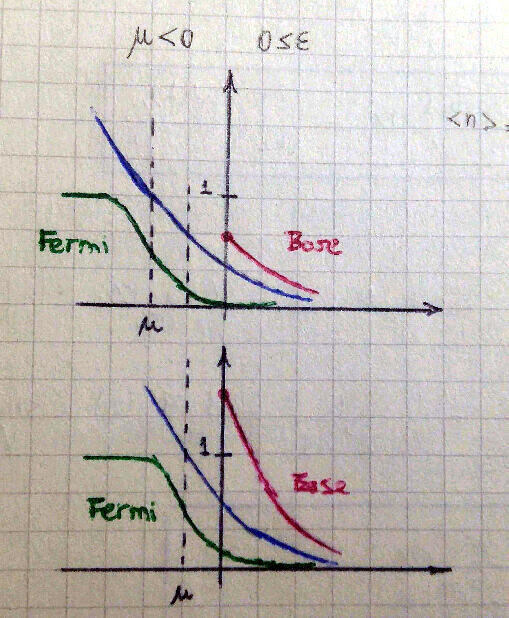
\includegraphics[scale=0.35]{images/1625623872.jpg}

Sea un sistema ideal de bosones $ \mu < 0 $ $ 0 \leq e $
\[
	\braket{n} = \frac{1}{ \euler^{-\beta\mu} \euler^{\beta e} - 1 }
\]
se tiene que para $ e=0 $ y $ \beta\mu = -1 $ es $ \braket{n} = $ 0.582 y para $ e=0 $ y $ \beta\mu = -0.5 $
es $ \braket{n} = $ 1.541

Vemos entonces que el condensado de Bose debe producirse con $ \mu \to 0^{-}$.

\section{Gases cuánticos}

Lo que sigue es un condensado de toda la teoría básica que ya está presente scattereada por aquí y allá.
Obviamente hay que curar y consolidar todo esto.

Se trabajará con gades ideales
\[
	H = \sum_i^N \: H_i
\]
o sea que consideramos no interacción con $N$ partículas indistinguibles. Si la $\Psi^N$ es antisimétrica
estaremos hablando de fermiones (estadística de Fermi-Dirac) y si es simétrica serán bosones, estadística
de Bose-Einstein.

Agregamos una estadística de Maxwell-Boltzmann (teórica). No tendrán una simetría dada; es una aproximación
de alta temperatura de un sistema cuántico.

El conteo de estados, ¿Cómo se realiza?
\begin{enumerate}
 \item Sobre microestados.
 \item Sobre energía $E$, según degeneración $g(E)$.
\end{enumerate}

Tendremos $ E = \sum_i^N \: e_i $ entonces podré factorizar si miro los niveles de energía de una partícula.
Un microestados será definido a través de los números de ocupación,
\[
	n_e = ( n_0, n_1, ..., n_j, ... )
\]
números de ocupación (cantidad de partículas en cada nivel energético). Se tienen 
\[
	\begin{cases}
		\sum_e \: n_e = N = n_0 + n_1 + ... + n_j + ... \\
		\sum_e \: e \: n_e = E
	\end{cases}
\]
y sabemnos que si son bosones se tendrá $n_e=0,1,2,...$ pero para fermiones $n_e=0,1$ (principio de exclusión,
dos partículas no pueden compartir sus números cuánticos). Para Boltzmann consideraremos $ n_e = 0, 1, 2, ...$
distinguibles y metemos el factor $ 1 / N! $. Entonces,
\[
	\begin{cases}
		g(n_e) = 1 \qquad \text{ f, b } \\
		g(n_e) = \frac{ N! }{ \Pi_e \: n_e! } \frac{ 1 }{ N! } \qquad \text{ MB }
	\end{cases} 
\]
pero esto no implica que no haya degeneración en la energía (los casos de fermiones y bosones).
\notamargen{En Bose las combinaciones que me puedo armar son las que harán la función de onda simétrica.}

Las funciones de partición 
\[
	Q_N(V,T) = \sum_{ \{n_e\} } \: \euler^{ -\beta E(n_e) } g(n_e),
\]
pero sujeta a que $ \sum n_e = N $. Para Maxwell-Boltzmann la $ g(n_e) $ quedará un binomio de Newton,
entonces $ Q_N = Q^N / N! $.

Para FD/BE la condición $ \sum n_e = N $ hace complicar la cuenta; nos vamos al gran canónico donde
es mucho más sencilla la cosa porque desaparece esa constraint y entonces
\[
	Q(z,V,T) = \sum_{N=0}^\infty \: z^N Q_N(V,T) =
	\sum_{N=0}^\infty \: z^N \sum_{ \{n_e\} } \: \euler^{ -\beta \sum_e \: e \: n_e }
\]
Se descorrelacionan los números de ocupación y 
\[
	\sum z^{n_0 + n_1 + ...} \sum \euler^{ -\beta ( \: e_0 \: n_0 + e_1 \: n_1 + ... ) } =
	\sum_{n_0} \: z {\euler^{-\beta e_0}}^{n_0} \: \sum_{n_1} \: z {\euler^{-\beta e_1}}^{n_1} ...
\]
y resulta
\[
	\prod ( \sum_{n} \: z {\euler^{-\beta e}}^{n} )
\]
donde $ n=0,1$ para fermiones y $n=0,1,2,...$ para bosones.
Entonces tendremos, respectivamente
\[
	Q(z,V,T) = \begin{cases}
		\displaystyle \prod_e \: \frac{1}{1-z\euler^{\beta e}} \\
		\\
		\displaystyle \prod_e \:  1 + z\euler^{-\beta e}
	\end{cases}
\]
donde en la primer expresión (bosones) se ha usado que $ | z \euler^{-\beta e} | < 1 $ para toda $e$.
\notamargen{Para gases ideales sin spin es $|z|<1$.}

\[
	\beta P V = \begin{cases}
		\displaystyle - \sum_e \: \log ( 1-z\euler^{\beta e} ) \\
		\\
		\displaystyle \sum_e \: \log( 1 + z\euler^{-\beta e} )
	\end{cases}
\]

\[
	N = \begin{cases}
		\displaystyle \sum_e \: \frac{1}{z^{-1}\euler^{\beta e} - 1 } \\
		\\
		\displaystyle \sum_e \: \frac{1}{z^{-1}\euler^{\beta e} + 1 }
	\end{cases}
\]

Recordemos que estamos sumando siempre sobre los niveles energéticos de una sola partícula (sus estados
cuánticos). El número medio de ocupación de cada nivel será
\[
	\vm{n_e} = \frac{1}{Q} \sum_{N=0}^\infty \: z^N \sum_{ \{ n_e\} } n_e \: \euler^{ -\beta \sum_e n_e e }
	= - \frac{1}{\beta} \dpare{ \log Q(z,V,T) }{e}{N,V,\text{ todos los otros $e$}} 
\]
\[
	\vm{n_e} = \frac{ 1 }{ z^{-1} \euler^{ \beta e } \mp 1 }
\]
siendo el primer signo para bosones y el segundo para fermiones.

\subsection{cuentas del paso discreto-continuo}

Consideramos la aproximación de que
\[
	p = \frac{2\pi\hbar}{\ell}( n_x, n_y, n_z ) \qquad \qquad 
	d^3p = \Frac{2\pi\hbar}{\ell}^3
\]
y esto último es el volumen por punto. Luego, el número de puntos por unidad de volumen es $ L^3/h^3 $.
Entonces,
\[
	\sum_p u  \longrightarrow \frac{L^3}{h^3} \int d^3p \longrightarrow  \frac{4 \pi L^3}{h^3} \int p^2 dp
\]
\notamargen{Si depende del módulo puede pasarse fácilmente a esféricas.}

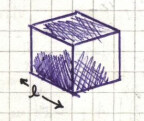
\includegraphics[scale=0.5]{images/1606329596.jpg}

Pero también puedo querer integrar en energía, entonces usamos $ m de = p dp $ que viene de $ e = p^2 / (2m)$
(relación de dispersión no relativista).
\[
	\frac{4 \pi L}{h^3} \int m \sqrt{ 2 m E } (\ldots) de = \int g(e) \: de (\ldots)
\]
donde la densidad de estados es
\[
	g(e) = \frac{4 \pi L}{h^3} m \sqrt{2 m E }.
\]

En $D=2$ dimensiones el factor que se hace cargo de los puntos en una superficie será $A^2$,
\[
	\frac{A^2}{h^2} \int d^2p (\ldots) \qquad  
	\frac{2 \pi A^2}{h^2} \int p dp (\ldots) = \frac{2 \pi A^2}{h^2} \int m de (\ldots)
\]
y entonces,
\[
	g(e) = \frac{2 \pi L^2}{h^2}m.
\]

En $D$ dimensiones tendremos $ g(e) \propto L^D e^{D/2-}$.

Recordemos que aquí siempre estamos en que $g(e)$ es el número de autoestados con energía comprendida
entre $e$ y $e+de$.







% \bibliographystyle{CBFT-apa-good}	% (uses file "apa-good.bst")
% \bibliography{CBFT.Referencias} % La base de datos bibliográfica

\end{document} 

	
		\documentclass[10pt,oneside]{CBFT_book}
	% Algunos paquetes
	\usepackage{amssymb}
	\usepackage{amsmath}
	\usepackage{graphicx}
% 	\usepackage{libertine}
% 	\usepackage[bold-style=TeX]{unicode-math}
	\usepackage{lipsum}

	\usepackage{natbib}
	\setcitestyle{square}

	\usepackage{polyglossia}
	\setdefaultlanguage{spanish}
	



	\usepackage{CBFT.estilo} % Cargo la hoja de estilo

	% Tipografías
	% \setromanfont[Mapping=tex-text]{Linux Libertine O}
	% \setsansfont[Mapping=tex-text]{DejaVu Sans}
	% \setmonofont[Mapping=tex-text]{DejaVu Sans Mono}

	%===================================================================
	%	DOCUMENTO PROPIAMENTE DICHO
	%===================================================================

\begin{document}

% =================================================================================================
\chapter{Gas de Fermi}
% =================================================================================================

DIBUJOS
\[
	\braket{n_e} = \frac{1}{z^{-1} \euler^{\beta e} + 1 } = \frac{1}{ \euler^{\beta ( \mu - e) } + 1 }
\]
Si $ \mu < 0 $ como $ e > 0 $ siempre, ni aún en el estado de más baja energía se llega a ocupar el
nivel (restan muchos niveles vacíos).

Sea que $ T \to \infty $ entonces $ \beta \to \infty $ y se sigue que 
\[
	\euler^{\beta(e-\mu)} \to \infty e> \mu
\]
\[
	\euler^{\beta(e-\mu)} \to 0 e< \mu
\]
\[
	\euler^{\beta(e-\mu)} \to 1 e = \mu
\]
Luego, con $ T = 0 $ es Fermi un escalón. El valor de $ \mu $ que determina el último
estado ocupado se llama $ e_F$ 

DIBUJO

\[
	f_{3/2}(z) = \frac{\lambda^3}{v} = \int_0^{\xi = \beta\mu } \frac{x^{1/2}}{\Gamma(3/2)3/2}dx =
	\frac{4}{3} \frac{1}{\pi^{1/2}} ( \beta\mu )^{3/2} = 
	\frac{4}{3} \frac{1}{\pi^{1/2}} ( \beta e_F )^{3/2}
\]

% =================================================================================================
\section{Análisis del gas ideal de Fermi}
% =================================================================================================

La primera aproximación consiste en 
\begin{itemize}
 \item Caso no degenerado : $\frac{\lambda^3}{v} \ll 1 $  que lleva a $ T $ alta y $ v $ alto
 por ende $ N/V $ chico.
 \[	
	z \ll 1 \qquad f_\nu(z) \approx z \qquad \frac{\lambda^3}{v} \approx z
 \]
 Si vale la condición entonces 
 \[
	\frac{\lambda^3}{v} = \sum_{l=1}^\infty \frac{(-1)^{l+1} z^l }{l^{3/2}} \ll 1 \qquad z \ll 1
 \]
 \[
	\beta p V \approx 1 + \frac{\lambda^3}{v 2^{5/2}} \qquad \qquad U = \frac{3}{2} \frac{N}{\beta}
	\left( 1 + \frac{\lambda^3}{v 2^{5/2}} \right)
 \]
 \item $\frac{\lambda^3}{v} < 1 $ entonces $ z < 1 $ y hay que expandir el virial,
 \[
	\beta p V = \sum_{l=1}^\infty (-1)^{l-1} a_l \left(\frac{\lambda^3}{v} \right)^{l-1}
 \]
 que igualando coeficientes se hace (¿?)
 \notamargen{ $\lambda^3 / v $ a orden 1 hay efectos cuánticos }
 \[
	f_{5/2}(z) = f_{3/2}(z) \cdot \sum_{l=1}^\infty (-1)^{l-1} a_l \left(\frac{\lambda^3}{v} \right)^{l-1}
 \]
 \item $\frac{\lambda^3}{v} \approx 1 $ Cálculo numérico
 \item Caso altamente degenerado : $\frac{\lambda^3}{v} \gg 1 $ se tiene $ z \gg 1 $ 
 Se puede expandir $ f_\nu(z) $ en función de $ (\log )^{-1} $ mediante lema de Sommerfeld
 \notamargen{ $ z \ggg 1 $ entonces $ \log z \gg 1 $ $ ( \log z )^{-1} \ll 1 $ $ \log z = \beta \mu $ }
 \[
	f_{5/2}(z) = \frac{8}{15\pi^{1/2}} (\log z)^{5/2} \left[ 1 + \frac{5\pi^2}{8}(\log z)^{-2} + ... \right]
 \]
 \[
	f_{3/2}(z) = \frac{4}{3\pi^{1/2}} (\log z)^{3/2} \left[ 1 + \frac{\pi^2}{8}(\log z)^{-2} + ... \right]
 \]
 y entonces
 \[
	\frac{\lambda^3}{v} = \frac{4}{3\pi^{1/2}} (\log z)^{3/2}  \quad \text{ a orden 0 }
 \]
 \[
	\frac{h^3}{ (2\pi mkT)^{3/2} } \frac{N}{V} \frac{3\pi^{1/2}}{4} (kT)^{3/2} = \mu^{ 3/2 }
 \]
 \[
	\frac{ h^3 }{ \pi } \frac{ N }{ V } \frac{ 3 }{ ( 2m )^{ 3/2 } 4 } = \mu^{ 3/2 } = e_F^{3/2}
 \]
 \[
	\frac{\lambda^3}{v}\frac{3\pi^{1/2}}{4} (kT)^{3/2} = 
	\mu^{3/2}\left[ 1 + \frac{\pi^2}{8}(\log z)^{-2} + ... \right]
 \]
 \[
	\frac{ h^3 }{ \pi } \frac{ N }{ V } \frac{ 3 }{ ( 2m )^{ 3/2 } 4 } = e_F^{3/2} \approx
	\mu^{3/2} \left[ 1 + \frac{\pi^2}{8}(\log z)^{-2} \right]
 \]
 \[
	e_F \approx \mu \left[ 1 + \frac{\pi^2}{8}( \frac{ \mu }{ kT } )^{-2} \right]^{ 2/3 } \approx 
	\mu \left[ 1 + \frac{\pi^2}{12} \Frac{ kT }{ \mu }^{2} \right]
 \]
 \notamargen{Anoté {\it investigar este pasaje}. }
 \[
	e_F \approx \mu \left[ 1 - \frac{\pi^2}{12}( \frac{ kT }{ e_F } )^{2} \right]
 \]
 y consideramos
 \[
	\frac{1}{\mu^2} \approx \frac{1}{e_F^2}
 \]
 pués $ \mu $ es muy grande.
 \[
	\beta p v = \frac{ f_{5/2}(z) }{ f_{3/2}(z) } \approx \frac{ 2 \beta \mu }{ 5 } 
	\left[ 1 + \frac{ 5\pi^2 }{ 8 } \left( \frac{kT}{\mu} \right)^2 \right]
	\left[ 1 - \frac{ \pi^2 }{ 8 } \left( \frac{kT}{\mu} \right)^2 \right]
 \]
 Hasta orden dos en $ T $ resulta 
 \[
	pv \approx \frac{ 2 \mu }{ 5 } \left[ 1 + \frac{ \pi^2 }{ 2 } \left( \frac{kT}{\mu} \right)^2 \right] =
	\frac{ 2 e_F }{ 5 }\left[ 1 - \frac{ \pi }{ 12 } \left( \frac{kT}{e_F} \right)^2 \right] 
	\left[ 1 + \frac{ \pi^2 }{ 2 } \left( \frac{kT}{e_F} \right)^2 \right] 
 \]
 \[
	pv \approx \frac{ 2 e_F }{ 5 } \left[ 1 + \frac{ 5 \pi^2 }{ 12 } \left( \frac{kT}{e_F} \right)^2 \right] 
 \]
 \[
	U = \frac{3}{2} p v \approx \frac{3}{5} N e_F 
	\left[ 1 + \frac{ 5 \pi^2 }{ 12 } \left( \frac{kT}{e_F} \right)^2 \right] 
 \]
 \[
	C_V = \dpar{U}{T} \approx \frac{ N \pi^2 k^2 T }{ 2e_F } \qquad C_V \propto T
 \]
 \[
% 	C_V \approx \frac{\pi^2}{2} Nk \left( \frac{T}{T_F} \right)
	C_V \approx \frac{\pi^2}{2} Nk \Frac{T}{T_F}
 \]
 DIBUJO 
 $T_F$ siempre estará ene general en la zona clásica donde no vale la aproximación degenerada.
 
 Calor específico Fermi (¿?)
 \item Caso totalmente degenerado : $\frac{\lambda^3}{v} \to \infty \qquad (T \to 0) \qquad z \to \infty $
 
 La distribución de estados es escalón,
 \[
	\braket{N} = \frac{ 4 \pi V }{ h^3 } \int_0^{p_F} p^2 \Frac{ 1 }{ z^{-1} \euler^{\beta p^2 / 2m } + 1} dp
 \]
 \notamargen{$ z = \euler^{\beta\mu} $ y $z(T\to 0) = \euler^{\beta e_F } \to \infty $}
 \[
	\braket{N} = \frac{ 4 \pi V }{ h^3 } \int_0^{p_F} p^2 dp
 \]
 
 Notemos que 
 \notamargen{Teniendo el límite sale la cuenta}
 \[
	pV = \frac{ 4 \pi V }{ h^3 } \int_0^{p_F} p^2 kT \log (1 + \euler^{ -1/kT( p^2/2m - \mu_0 )} ) dp
 \]
 tiene un comportamiento no trivial con $ T \to 0 $. Si $ kT \to 0 $ entonces si $e > \mu_0$ el $\log \to 0$
 y si $e < \mu_0$ el $\log \to \infty $.
 Parecería que con $ T \to 0 $ es
 \[
 	pV = \frac{ 4 \pi V }{ h^3 } \int_0^{p_F} p^2 \left( \frac{ p^2 }{ 2m } - \mu_0 \right) dp
 \]
 y haciendo el cambio de variables de acuerdo a $ p^2 / 2m = e $, que lleva a $ pdp = m de $, se tiene 
 \[
 	pV = \frac{ 4 \pi V }{ h^3 } \int_0^{e_F} \sqrt{2e} m^{3/2} ( e -\mu_0 ) de
 \]
 \[
	pV = \frac{ 4 \pi V }{ h^3 } 2^{ 1/2 } m^{ 3/2 } 
	\left( \frac{e_F^{ 5/2 }}{5/2} - \mu_0 \frac{e_F^{ 5/2 }}{3/2} \right) =
	\frac{ 4 \pi V }{ h^3 }2^{ 1/2 } m^{ 3/2 } e_F^{ 5/2 } \frac{ 4 }{ 15 }
 \]
 \[
	U = \frac{3}{2} p V = \frac{ 4 \pi V }{ h^3 }2^{ 1/2 } m^{ 3/2 } e_F^{ 5/2 } \frac{ 2 }{ 5 }
 \]
 \[
	p = \frac{2}{5} e_F \frac{\braket{N}}{V} \qquad U = \frac{3}{5} e_F \braket{N} 
 \]
 A $ T = 0 $ tenemos presión y energía no nulas; las partículas no se acomodan todas en un único nivel energético
 (exclusión de Pauli).
 Para $ T \approx 0 $ ( $T$ bajas) el escalón en estados apenas se desdibuja
 
 DIBUJO.
 
\end{itemize}

% =================================================================================================
\section{Cuánticos III --reubicar--}
% =================================================================================================
 
 \subsection{Los números de ocupación}
 
 DIBUJO
 
 Se ve que para Bose $ \mu < 0 $ siempre pero $ \braket{n} \to \infty $ si $ \mu \to 0^+ $.
 El gráfico es para $T$ alta. Con $ T $ bajas todo tiende a suceder más pegado al eje $ \beta(e-\mu) = 0 $
 
 \subsection{Comportamiento de $ f_{3/2}(z) $}
 
 \[
	f_{3/2}(z) = \sum_{j=1}^\infty (-1)^{j+1}\frac{z^j}{j^{3/2}} \approx z - \frac{z^2}{2^{3/2}} \qquad 
	\text{ $z$ chico }
 \]
 \[
 	f_{3/2}(z) = \frac{1}{\Gamma(3/2)} \int_0^\infty \frac{x^{1/2}}{z^{-1}\euler^{x} + 1} dx \approx  
 	\frac{1}{\Gamma(3/2)} \int_0^{\log z = \beta\mu} x^{1/2} dx
 \]
 
Notemos que con $ \beta \mu $ grande el integrando es 1 o 0 (DIBUJO); en realidad es un escalón en el límite
en que $ \xi \equiv \beta\mu \to \infty$
\notamargen{Definimos $ \log z \equiv \xi $ para no especular con temperaturas. }

\[
	f_{3/2}(z) = \frac{4}{ 3 \sqrt{\pi} } (\log z )^{3/2} \text{ $z$ muy alto }
\]
\[
	f_{3/2}(z) = \frac{4}{ 3 \sqrt{\pi} } \left[ (\log z )^{3/2} + \frac{\pi^2}{8}(\log z )^{-1/2} + ... \right]
\]

El valor $ \lambda^3 / v $ determina relación entre $ T,V,N $ que son los parámetros macroscópicos que uno fija.

\subsection{Casos}

\begin{itemize}
 \item Comportamiento clásico: $\frac{\lambda^3}{v} \ll 1$ Altas $T$ y bajas $n\equiv \frac{N}{V}$ 
 \[
	\frac{\lambda^3}{v} = f_{3/2}(z) \approx z - \frac{z^2}{2^{3/2}}
 \]
 y por inversión de la serie 
 \[
	z = \frac{\lambda^3}{v} + \Frac{\lambda^3}{v}^2 2^{-3/2}
 \]
 \notamargen{Sabemos que en Boltzmann es $\frac{\lambda^3}{v} = z$ }
 y entonces si $\frac{\lambda^3}{v} \ll 1$ se tiene que $ z \ll 1 $
 \[
	\frac{pv}{kT} = \frac{v}{\lambda^3} f_{5/2}(z) \qquad \qquad \frac{\lambda^3}{v} = f_{3/2}(z)
 \]
 \[
	\frac{pv}{kT} = \frac{f_{5/2}(z)}{f_{3/2}(z)} \approx \frac{z - z^2/2^{5/2}}{z - z^2/2^{3/2}}
	\approx 1 + \frac{1}{2^{3/2}} \Frac{\lambda^3}{v}
 \]
 siendo el último término una corrección cuántica.
 
  \item Comportamiento cuántico : $\frac{\lambda^3}{v} \gg 1$ Bajas $T$ y altas $n\equiv \frac{N}{V}$ 
  
  A $ T = 0 $ determinamos la $ e_F $ como (con el límite de $T\to 0$)
  \[
	\frac{\lambda^3}{v} = \frac{1}{\Gamma(3/2)} \int_0^{\log z = \beta\mu} x^{1/2} dx = 
	 \frac{4}{ 3 \sqrt{\pi} } (\log z )^{3/2}
  \]
  \[
	\Frac{ 3  \lambda^3  \sqrt{\pi} }{4v}^{2/3} = \Frac{ 3  h^3  \sqrt{\pi} }{4(2\pi m k T)^{3/2}v}^{2/3} 
	= \log z =  \beta e_F
  \]
  \[
	\frac{h^2}{2m}\Frac{3}{4\pi v}^{2/3} = e_F = \frac{\hbar}{2m}\Frac{6\pi^2}{v}^{2/3}
  \]
  A $ T = 0 $ la ocupación por nivel es un escalón ($e_F = \mu(T=0) $) 
  \[
	\braket{n_e} = 	\begin{cases}
			1 \qquad e < e_F \\
			0 \qquad e > e_F
			\end{cases}
  \]
\end{itemize}

\subsection{Funciones termodinámicas con $T$ baja y $n$ alta}

Usamos Sommerfeld
\[
	\frac{\lambda^3}{v} = f_{3/2}(z) \qquad  \qquad \mu = e_F
\]
orden 1
\[
	\frac{\lambda^3}{v} =  
	\frac{4}{3\sqrt{\pi} } (\log z )^{3/2} \left[ 1 + \frac{\pi^2}{8}(\log z )^{-2} \right] 
\]
\[
	\frac{\lambda^3}{v} \frac{3\sqrt{\pi} }{4} \left[ 1 + \frac{\pi^2}{8}(\log z )^{-2} \right]^{-1} 
	\approx (\log z)^{3/2} 
\]
\[
	e_F \left( 1- \frac{\pi^2}{12}\Frac{T}{T_F}^2 \right) \approx \mu( T ) \text{ cumple $\mu(T=0)=e_F$}
\]
Puede verse que con $ \frac{\lambda^3}{v} \ggg 1 $ ($T$ baja y $n$ alta) es
\[
	C_V \approx \frac{N \pi^2 k^2 T}{2 e_F}
\]
DIBUJO

Aún a $T=0$ hay presión no nula pero $S \to 0$ con $T \to 0$ respetando la tercera ley.
Existe una relación de recurrencia
\[
	z\dpar{}{z} f_\nu(z) = z\dpar{}{z} \sum_{l=1}^\infty (-1)^{l+1} \frac{z^l}{l^\nu} =
	\sum_{l=1}^\infty (-1)^{l+1} \frac{l z^{l-1} z}{l^\nu} = 
	\sum_{l=1}^\infty (-1)^{l+1} \frac{z^l}{l^{\nu-1}} = f_{\nu-1}(z)
\]
\[
	f_\nu(z) = \int \frac{1}{z} f_{\nu-1}(z) dz
\]
\[
	f_{3/2}(z) \approx \frac{4}{3\sqrt{\pi}} (\log z)^{5/2}
\]
entonces
\[
	f_{5/2}(z) = \int dz \frac{4}{3\sqrt{\pi}} \frac{(\log z)^{3/2}}{z} =
	 \frac{4}{3\sqrt{\pi}} \int dz \frac{ 2 }{ 5 } \dpar{}{z} (\log z)^{5/2} =
	\frac{8}{15\sqrt{\pi}}(\log z)^{5/2}
\]
\notamargen{Usamos $d(\log z)^n = n (\log z)^{n-1}/z $}

\subsection{Sobre la aproximación de gas de Fermi para el núcleo}

En lo que sigue una deducción más detallada del cálculo.
Considero una caja de lados $L$
\[
	\vb{k} = \frac{2\pi}{L} \vb{n} \qquad \hbar \vb{k} = \vb{p} = \frac{h}{L} \vb{n}
\]
\notamargen{Tomo en el origen de coordenadas $n_i = \pm 1, \pm 2, ...$ y así voy de $-L/2$ a $L/2<$.}
\[
	E = \frac{( \hbar |\vb{k}| )^2}{ 2m } = \frac{ \hbar^2 }{ m } \frac{2\pi^2}{L^2}
	(n_x^2 + n_y^2 + n_z^2) \qquad n_i \in \mathbb{Z}
\]
Quiero saber qué densidad de estados energéticos tengo. Para ello, en esféricas
\[
	E = \frac{ \hbar^2 }{ m } \frac{2\pi^2}{L^2} r^2
\]
donde $r$ vive en la esfera (no es necesario tomar el octante y dividir sobre 8)
\[
	g(E) dE = N(r) dr = 4\pi r^2 dr
\]
siendo $g(E) dE$ el número de puntos entre $E$ y $E+dE$,
\[
	dE = \frac{(\hbar \pi)^2}{L^2 m}4 r dr 
\]
\[
	g(E) dE = \frac{ L^3 m^{3/2} E^{1/2} }{ \hbar^{3/2} \pi^2  \sqrt{2}}dE
\]
\[
	N = g\int_0^{e_F} g(E) dE = \sqrt{2} \frac{ V m^{3/2} }{ \hbar^3 \pi^2 } 
	\int_0^{e_F} e^{1/2} dE
\]
\[
	N = \frac{ V m^{3/2} }{ \hbar^3 \pi^2 } \frac{2^{3/2}}{3} e_F^{3/2}
\]
\[
	\frac{1}{v} = \frac{ m^{3/2} }{ \hbar^3 \pi^2 } \frac{2^{3/2}}{3} e_F^{3/2}
\]
y entonces deducimos de aquí que 
\[
	e_F = \frac{\hbar}{2m} \Frac{3\pi^2}{v}^{2/3}
\]
que coincide con la expresión para $e_F$ con degeneración $g=2$

\notamargen{¿Y estas cuentas sueltas?}
\[
	n_x^2 + n_y^2 + n_z^2 = r^2 \qquad V=\frac{4}{3}\pi r^3 \qquad dV = 4\pi r^2 dr
\]
\[
	E = \frac{(\hbar \pi)^2}{2ma^2}r^2 \qquad \qquad dE = \frac{(\hbar \pi)^2}{ma^2}r dr
\]
\[
	N(r) dr = \frac{\pi}{2} r^2 dr 
\]
será lo mismo que el incremento en niveles energéticos
\[
	N(e)de = \frac{m^2 a^3}{\pi^2 \hbar^3} \Frac{E}{2}^{1/2} dE
\]
Pensamos un conjunto de nucleones como un gas de Fermi. 
\notamargen{Recordemos que a $T=0$ era $pV=2/5 N e_F$ y $U=3/5 N e_F$}
Claramente
\[
	N = 2 \int_0^{e_F} N(e) \; de
\]
porque tenemos la ocupación en función de la energía
\[
	e_F \propto \Frac{N}{V}^{2/3} \text{ según la definición de $e_F$ }
\]

Al aplicar este modelo (del gas de Fermi) al núcleo hacemos algunas consideraciones
\[
	R = a_0 A^{1/3} \qquad V \propto A 
\]
siendo $A$ el número de nucleones.

Para un núcleo se tienen N=A-Z neutrones, siendo Z protones y A nucleones.
\[
	E = \frac{3}{5}N_Te_F (\text{ a } T=0)
\]
y tenemos un $e_F$ de protones y de neutrones, que son 
\[
	e_{Fp} \propto \Frac{Z}{A}^{2/3} \qquad \qquad 
	e_{Fn} \propto \Frac{A-Z}{A}^{2/3}
\]
\[
	E = \frac{3}{5}\left[ Z\Frac{Z}{V}^{2/3} + (A-Z)\Frac{A-Z}{V}^{2/3} \right] =
	\frac{3}{5}\Frac{ Z^{5/3} + (A-Z)^{5/3} }{A^{2/3}}
\]
donde hemos supuesto ambos pozos iguales. Si los pozos no fueran iguales cambia la
$e_F$.

Se minimiza $E$ con $Z=N=A/2$ (simetría)
\[
	f_4 \propto E-E_0 = \frac{3}{5A^{2/3}} \left[ Z^{5/3} + (A-Z)^{5/3} - 2(A/2)^{5/3} \right]
\]
que se puede reescribir en función de $D = (N-Z)/2 = (A - 2Z)/2 = A/2 - Z$ (que será chico) y
de esta manera 
\[
	Z = \frac{A}{2} - D \qquad A-Z = \frac{A}{2} + D
\]
\[
	f_4 \propto \frac{3}{5} \left( \frac{ [A/2 - D]^{5/3} + [A/2 + D]^{5/3} - 2[ A/2 ]^{5/3} }{A^{2/3}}\right)
\]
y que con un Taylor en $ D \approx 0 $ resulta 
\[
	f_4 \propto \frac{(A/2 - Z)^2}{A} \propto D^2 \text{ término de simetría }
\]

\subsection{Cuánticos 3 -- más material para reubicar--}

Un esquema de temas:
comportamiento de los números de ocupación
gas de Fermi : comportamiento de $f_\nu(z)$ con $ \nu = 3/2 $
gas de Fermi con condiciones extremas
\[
	\lambda^3 / v \ggg 1 \qquad \qquad \lambda^3 / v \lll 1
\]
$e_F$ con degeneración $g$
funciones termodinámicas con $\lambda^3 / v \ggg 1$ $ S \to 0 $ con $ T\to 0$
Aproximación de gas de Fermi para núcleo
densidad de estados $g(e)$


La expresión para $ \mu(T) $ con $ T \geq 0 $ sale de 
\[
	\frac{\lambda^3}{v} =  
	\frac{4}{3\sqrt{\pi} } (\log z )^{3/2} \left[ 1 + \frac{\pi^2}{8}(\log z )^{-2} \right] 
\]
\[
	( \log z )^{3/2} = \frac{ 3\sqrt{\pi} h^3 }{ ( 2 \pi m )^{3/2} (kT)^{3/2} 4v }   
	\frac{1}{\left[ 1 + \frac{\pi^2}{8}(\log z )^{-2} \right] }
\]
\[
	\mu = \Frac{3 \sqrt{\pi} }{4v}^{2/3} \frac{h^2}{2\pi m}
	\left( 1 + \frac{\pi^2}{8\log^2 z}\right)^{-2/3}
\]
\[
	\mu = e_F \left[ 1 - \frac{\pi^2}{12} \Frac{kT}{e_F}^2 \right]
\]
y con $T$ baja podemos escribir todo en función de la $e_F$.
\notamargen{Hay un yeite en la deducción que refiere a que abajo es lo mismo usar orden 1 que
orden dos y reemplazo $ (\beta \mu)^{-2} $ por $(\beta e_F)^{-2}$}
\[
	E = \frac{3}{5}Ne_F \qquad \qquad \text{ con } T=0
\]

Lo importante de tener $ f_{3/2}(z) $ en función de $ \lambda^3/v $, desde 
\[
	 \lambda^3/v  = f_{3/2}(z) 
\]
DIBUJO

es que vemos que $z$ chico lleva a $ \lambda^3/v $ grande y consecuentemente $z$ grande lleva a
$ \lambda^3/v $ grande.

Luego,
\begin{multline*}
	\text{ clásico } z \ll 1 \\
	\frac{ \lambda^3 }{ v } \ll 1 \text{ independientemente }
\end{multline*}
\begin{multline*}
	\text{ cuántico } z \gg 1 \\
	\frac{ \lambda^3 }{ v } \gg 1 \text{ independientemente }
\end{multline*}

Con $ T=0$ es $\mu(T=0)=e_F$
DIBUJO escalón

Cuántico (límite máximo) entonces
\[
	z \to \infty \Rightarrow \frac{ \lambda^3 }{ v } = \frac{4(\log z)^{3/2}}{3\sqrt{\pi}}
\]
\[
	\frac{ \lambda^3 }{ v } = \frac{4}{2\sqrt{\pi}}(\beta e_F)^{3/2} \text{ con } z=\euler^{\beta e_F}
\]

Entonces $e_F$ es el nivel tal que debajo de él hay N estados. En el espacio de momentos las partículas
ocupan una esfera de radio $p_F$.


\subsection{Estadísticas --otra cosa para reubicar--}

Esta sección es un sketchi

\[
	\braket{n}_i = \frac{1}{ \euler^{\beta(e_i - \mu)} + a} \qquad \qquad 
	\begin{cases}
	 a = 0 \quad \text{ MB } \\
	 a = -1 \quad \text{ BE } \\
	 a = 1 \quad \text{ FD } 
	\end{cases}
\]

DIBUJO 

Graficamos $1/ \euler^x + a $
En la zona clásica coinciden las tres y es
\[
	\euler^{\beta (e_i - \mu)} \gg 1 \forall e_i \; \text{ de interés }
\]
\[
	z^{-1} \euler^{\beta e_i } \gg 1 \qquad \qquad \beta(e_i - \mu) \gg 0
\]
\[
	\euler^{\beta e_i } \gg z \qquad \qquad e_i \gg \mu
\]
de (2) se deduce que como $e_i$ pueden ser $\approx 0$ entonces $0\gg\mu$ y por lo tanto
$\euler^{\beta\mu} \equiv z \ll 1$ de (1)
\[
	1 \gg \euler^{\beta\mu} \qquad \qquad 0 \gg \beta\mu
\]

Clásicamente $\euler^{\beta\mu}$ domina sobre $z$
\[
	\mu < 0 \text{ y } |\mu| \gg 1 
\]
\[
	\text{ Bose } \mu < \text{ todo } e
\]
\[
	\text{ Fermi } \mu \text{ sin restricción }
\]


Para $ z \ggg 1 $ conviene definir $ \xi = \log z $ y entonces 
\[
	f_\nu(z) = \frac{1}{\Gamma(\nu)} \int_0^\infty \frac{x^{\nu-1}}{\euler^{x-\xi}+1} dx
\]

Siendo $\xi$ grande se tendrá que 
\[
	F = \frac{ 1 }{ \euler^{x-\xi} + 1 } = \begin{cases}
	                  1 \qquad x < \xi \\
	                  1/2 \qquad x=\xi \\
	                  0 \qquad z > \xi
	                 \end{cases}
\]
En este supuesto $ \xi \ggg 1 $ podemos integrar
\[
	f_\nu(z) \approx \frac{1}{\Gamma(\nu)} \int_0^\infty x^{\nu-1} dx
\]
donde suponemos $ T \gtrsim 0 $ con lo cual $ \beta\mu \to \infty, \xi \to \infty$ y 
$z^{-1} \to 0, \euler^{-\xi} \to 0$

\[
	f_\nu(z) \approx \frac{ \xi^\nu }{\Gamma(\nu) \nu}
\]

Con $ \nu = 3/2 $ resulta 
\[
	f_{3/2}(z) \approx \frac{ (\log z)^{3/2} }{\Gamma(3/2) 3/2}
\]
\[
	\frac{\lambda^3}{v} = \frac{4}{3} \frac{1}{\pi^{1/2}}(\beta\mu)^{3/2} \to
	\left( f_{3/2}(z) \frac{3\sqrt{\pi}}{4}\right)^{2/3} \frac{1}{\beta} = e_F
\]
\[
	\frac{h^2}{2m} \Frac{3}{4v\pi}^{2/3} = \mu = e_F (\mu \text{ a } T=0 )
\]

La $e_F (\mu \text{ a } T=0 )$ es la energía hasta la cual se hallan ocupados los
niveles energéticos. Con $ T \gtrsim 0$ la ocupación es un escalón

DIBUJO 

La $e_F$ es el valor de $\mu (T=0)$

La energía $U$ es 
\[
	U  = \frac{3}{2} p V = \frac{3V}{2\beta\lambda^3} f_{3/2}(z) = \frac{3N}{2\beta} \frac{f_{5/2}(z)}{f_{3/2}(z)}
\]

Tenemos una aproximación de Sommerfeld para $z$ grande 
\[
	f_{3/2}(z) = \frac{ 4 }{ 3\sqrt{\pi} } (\log z)^{3/2} \left[ 1 + \frac{\pi^2}{8}(\log z)^{-2} + ... \right]
\]
\[
	f_{5/2}(z) = \frac{ 8 }{ 15\sqrt{\pi} } (\log z)^{5/2} \left[ 1 + \frac{5\pi^2}{8}(\log z)^{-2} + ... \right]
\]
\[
	U = \frac{ 3N }{ 5\beta } (\log z) 
	\left[ 1 + \frac{5\pi^2}{8}(\log z)^{-2} + ... \right]
	\left[ 1 + \frac{\pi^2}{8}(\log z)^{-2} + ... \right]^{-1}
\]
\[
	U = \frac{3\mu}{5} \left[ 1 + \frac{5\pi^2}{8}(\log z)^{-2} + ... \right] =
	\frac{3\mu}{5} + \frac{15\pi^2\mu}{60} \Frac{1}{\beta\mu}^2 + ...
\]
\[
	C_v \equiv \dpar{}{T}U/N \cong \frac{\pi^2}{2} \frac{k^2 T}{\mu}
\]
entonces con $T \gtrsim 0$ es $C_v \propto T$ y con $T=0$ es
\[
	\frac{ U}{N} = \frac{3}{5} e_F
\]
\[
	\frac{ U}{N} = \frac{3}{5} e_F \left( 1 + \frac{5\pi^2}{12} 
	\Frac{T}{\underbrace{e_F/k}_{\equiv T_F}}^2 + ... \right) 
\]

Para $z \approx 1$ se debe expandir en el virial
\[
	\frac{pV}{NkT} = \sum_{l=1}^\infty a_l \Frac{\lambda^3}{gv}^{l-1} (-1)^{l-1}
\]

Sabemos que 
\[
	\frac{p}{kT} = \frac{f_{5/2(z)}}{\lambda^3}
\]
y entonces con las expresiones de $f_\nu$,
\[
	\frac{pV}{NkT} = \frac{ \sum_{j=1}^\infty (-1)^{j+1} z^j / j^{5/2} }
	{ \sum_{k=1}^\infty (-1)^{k+1} z^k / k^{3/2} }
\]

Debemos usar toda la serie 
\[
	\left[ \sum_{l=1}^\infty a_l \Frac{\lambda^3}{gv}^{l-1} (-1)^{l-1} \right]
	\left[ \sum_{k=1}^\infty (-1)^{k+1} z^k / k^{3/2} \right] =
	\sum_{j=1}^\infty (-1)^{j+1} z^j / j^{5/2}
\]

Resultan
\[
	\begin{cases}
	 a_1 = 1 \\
	 a_2 = -0.17678 \\
	 a_3 = -0.00330
	\end{cases}
\]
\[
	\frac{pV}{NkT} = 1 + 0.17678 \underbrace{\Frac{\lambda^3}{gv}}_{\propto T^{-3/2}} 
	- 0.00330\Frac{\lambda^3}{gv}^2
\]

Usando 
\[
	U = 3/2 p V
\]
\[
	\frac{U}{N} \cong 3/2 kT \left( 1 + 0.17678 \Frac{\lambda^3}{gv} \right)
\]
\[
	\dpar{}{T} \frac{U}{N} = C_v = 3/2 kT \left( 1 + 0.17678 \Frac{\lambda^3}{gv} \right)
	+ \frac{3}{2} kT 0.17678 \frac{h^3}{gv(2\pi mk)^{3/2}2/3 T^{5/2}}
\]
y se puede despejar
\[
	c_v = \frac{3}{2} k \left[ 1- 0.08839 \Frac{\lambda^3}{gv}  \right]
\]

% =================================================================================================
\section{Estudio de un metal -- título tentativo --}
% =================================================================================================

\subsection{Estudio de un metal}

Modelamos un metal como una red de átomos que pueden oscilar y un gas de electrones
\[
	(\vb{x}_1, ...,\vb{x}_N ) \qquad \qquad \text{ $N$ átomos }
\]
\[
	(\vb{x}_1^0, ...,\vb{x}_N^0 ) \qquad \qquad \text{ Equilibrio fundamental }
\]

PICTURE 

Los desplazamientos del equilibrio serán 
\[
	\vb{x}_i - \vb{x}_i^0 = \vec{\xi}_i
\]
\notamargen{Planteo de un potencial de pequeñas oscilaciones}
\[
	K = \sum_i \frac{m}{2} | \vec{\xi}_i|^2 \qquad \text{ cinética }
\]
\[
	V = V(\{ \vb{x}_i^0 \}) + \sum_i \underbrace{\left. \dpar{V}{\vb{x}_i}\right|_{\vb{x}_i}}_{=0}
	(\vb{x}_i-\vb{x}_i^0) + 
	\sum_{i,j} \frac{1}{2} \dpar{V}{\vb{x}_i}{\vb{x}_j} (\vb{x}_i-\vb{x}_i^0) (\vb{x}_j-\vb{x}_j^0)
\]
\notamargen{Es cero porque está evaluado en el mínimo.}
\[
	V = V_0 + \sum_{i,j} \frac{1}{2} k_{ij}  \vec{\xi}_i\cdot  \vec{\xi}_j \qquad \text{ potencial }
\]
siendo las constantes de fuerza $k_{ij}$ las que controlan la interacción 
\[
	H = V_0 + \frac{m}{2} | \vec{\xi}_i|^2  + \sum_{i,j} \frac{1}{2} k_{ij}  \vec{\xi}_i\cdot  \vec{\xi}_j
\]

Este hamiltoniano se puede pasar a modos normales diagonalizando la matriz de fuerzas
\[
	H = V_0 + \frac{m}{2}  \sum_i^{3N} \left( \dot{q}_i^2 + \omega_i^2 q_i^2 \right)
\]
y $\omega_i$ son las frecuencias de los $3N$ modos normales del sistema de $N$ grados de libertad en
3D. En modos normales el hamiltoniano del sistema es el de $3N$ osciladores armónicos independientes
(no acoplados. 
Puede resolverse mediante los operadores de bajada y de subida (cuántica) resultando en
\[
	E = \sum_i^{3N} \left( n_i + \frac{1}{2} \right) \hbar \omega_i
\]
donde $n_i$ es el número de fonones (ocupación) del modo normal $i-$ésimo.

Estos fonones, cuasipartículas, son bosones porque pueden ser 
\[
	n_i = 0,1,2,...,\infty
\]
y su número total no está fijo ($\mu=0$ pues la energía no depende del número de fonones)
\[
	n_i = \frac{1}{\euler^{\beta\hbar \omega_i} -1 }
\]
pues $\hbar\omega_i$ es la energía del estado $i-$ésimo
\[
	n_i = \frac{1}{\euler^{ \hbar \omega_i / kT } -1 }
\]
\[
	E = V_0 + \frac{1}{2} \sum_i^{3N} \hbar \omega_i + \sum_i^{3N} n_i \hbar \omega_i
\]

La función de partición canónica será 
\[
	Q = \sum_E \euler^{ -\beta E } =
	\sum_E \euler^{ -\beta \left( \frac{1}{2} \sum \hbar \omega_i + \sum n_i \hbar \omega_i \right) }
\]
\[
	Q = \sum_{n_1=0}^\infty \sum_{n_2=0}^\infty ... \sum_{n_N=0}^\infty 
	\euler^{ -\beta \sum \left( \hbar \omega_i /2  + n_i \hbar \omega_i \right) }
\]
\[
	Q = \sum_{n_1} \euler^{ -\beta \left( \hbar \omega_1 /2 + n_1 \hbar\omega_1 \right) }
	\sum_{n_2} \euler^{ -\beta \left( \hbar \omega_2 /2 + n_2 \hbar\omega_2 \right) } \; ...
\]
\[
	Q = \prod_i^{3N} \left(
	\sum_{n_i=0} \euler^{ -\beta \left( \hbar \omega_i /2 + n_i \hbar\omega_i \right) } 
	\right) = \prod_i^{3N} \left(
	\sum_{n_i=0} \euler^{ -\beta n_i \hbar\omega_i } \right) \euler^{ -\beta \hbar \omega_i /2 }
\]
\[
	Q = \prod_i^{3N} \left(
	\frac{1}{1-\euler^{ -\beta \hbar \omega_i } } \right)  \euler^{ -\beta \hbar \omega_i /2 } = 
	\prod_i^{3N} \left( \frac{1}{ \euler^{ \beta \hbar \omega_i } -\euler^{ -\beta \hbar \omega_i } } \right)
\]
\[
	\log Q = \sum_i^{3N} \log \left( \frac{1}{ \euler^{ \beta \hbar \omega_i } -\euler^{ -\beta \hbar \omega_i } } 
	\right) = 
	\sum_i^{3N} - \log \left( { \euler^{ \beta \hbar \omega_i } -\euler^{ -\beta \hbar \omega_i } } \right)
\]
\[
	\log Q = \sum_i^{3N} - \log \left( 2 \sinh \Frac{\hbar\omega_i}{2kT} \right)
\]

Si quisiéramos pasar al continuo resultaría (con $N \to \infty$)
\[
	\log Q = - \int_0^\infty d\omega g(\omega) \log \left[ 2 \sinh \Frac{\beta\hbar\omega_i}{2} \right]
\]
donde $ g(\omega) $ es la densidad de estados y 
\[
	d\omega g(\omega) = \text{ \# de modos normales con frecuencia entre $\omega$ y $\omega + d\omega$ }
\]

Tenemos dos métodos de cálculo de energía
\begin{center}
\begin{tabular}{l|l}
$ \displaystyle E = \sum_i^{3N} ( n_i + 1/2 )\hbar\omega_i $ & 
$ \displaystyle -\dpar{\log Q}{\beta} = \sum_i^{3N} \frac{1}{\euler^\Box - \euler^{-\Box}}( \euler^\Box + 
\euler^{-\Box} )\frac{\hbar\omega_i}{2} $ \\
& \\
$ \displaystyle \sum_i^{3N} \hbar\omega_i\Frac{1/2\euler^{\beta\hbar\omega_i}+1/2}{\euler^{\beta\hbar\omega_i}-1} $  & 
$ \displaystyle -\dpar{\log Q}{\beta} = \sum_i^{3N} \Frac{\euler^\Box + \euler^{-\Box}} {\euler^\Box - \euler^{-\Box}} 
\frac{\hbar\omega_i}{2} $ \\
& \\
$ \displaystyle \sum_i^{3N} \frac{\hbar\omega_i}{2}\Frac{\euler^{\beta\hbar\omega_i}+1}{\euler^{\beta\hbar\omega_i}-1} $ 
& $ \displaystyle = \sum_i^{3N} \Frac{\euler^{2\Box} + 1 }{ \euler^{2\Box} - 1 } \frac{\hbar\omega_i}{2} $ \\
\end{tabular}
\end{center}

Por supuesto ambas coinciden. Observemos que 
\[
	\text{ \# de fonones } = \sum_i^{3N} n_i
\]
es una cantidad que no es fija (se crean y se destruyen). Por ello podemos evaluar fácilmente el
$Q$.

Desde $E$ se puede evaluar el $C_v$
\[
	\dpar{E}{T} = \sum_i^{3N} \frac{\hbar\omega_i}{2} \dpar{}{T}\Frac{ \cosh \Box }{ \sinh \Box } 
\]
\[
	C_v = \sum_i^{3N} \frac{\hbar\omega_i}{2} \left[ 
	\frac{ \sinh \Box }{ \sinh \Box }\dpar{\Box}{T} - \frac{ \cosh^2 \Box }{ \sinh^2 \Box } \dpar{\Box}{T}
	\right]
\]
\[
	C_v = \sum_i^{3N} \frac{\hbar\omega_i}{2}  \frac{\hbar\omega_i}{2k} \Frac{-1}{T^2} 
	\Frac{-1}{\sinh^2 \Box}
\]

Tenemos el modelo de Einstein, que usa $ \omega_i = \omega_E \forall i $ y entonces 
\[
	C_v = 3N k \Frac{\hbar\omega_E}{kT}^2 \frac{1}{[\euler^{\hbar\omega_E/kT2} -\euler^{-\hbar\omega_E/kT2}]^2}
\]
\[
	C_v = 3Nk \left[ \Frac{1}{t}^2 \Frac{1}{\euler^{1/(2t)}-\euler^{-1/(2t)} }^2 \right]
\]

Con $ T \ggg 1 $ es $ [ ... ] \to 1$ y $C_V = 3Nk $ (clásico). Con $ T < 1 $ se comporta exponencialmente.

Dibujo 

$ C_v \to 3Nk $  con $ T \ggg 1 $, $ C_v \to 0 $ con $ T \to 0 $ Tiende a cero muy rápidamente

\subsection{Modelo de Debye}

Las frecuencias se distribuyen continuamente de modo que hay 
\[
	\int_0^{\omega_D} g(\omega) d\omega = 3N
\]
modos normales; es decir que se integra hasta una frecuencia de corte $\omega_D$. $g(\omega)$ la extraemos de 
considerar frecuencias permitidas de una onda plana de sonido en un sólido de lados $L$.
\[
	\vb{p} = \frac{h}{L}\vb{n} = \frac{h}{2\pi}\vb{k} \qquad \rightarrow  \qquad \vb{k} = \frac{2\pi}{L}\vb{n}
	\qquad \delta |\vb{k}| = \frac{(2\pi)^3}{V}
\]
\[
	c_s = \frac{\omega}{|\vb{k}|} \qquad \rightarrow \qquad  4 \pi k^2 \frac{V}{(2\pi)^3} dk = 1 \text{ esféricas }
\]
\[
	d|\vb{k}| = \frac{d\omega}{c_s}
\]
y será 
\[
	\frac{V}{2\pi^2} k^2 dk = \frac{V}{2\pi^2} \frac{\omega^2}{c^3} d\omega
\]
\[
	g(\omega) d\omega = g(k) dk \quad \rightarrow \quad g(\omega) = \frac{V\omega^2}{2\pi^2c^3}
\]
\[
	\int_0^{\omega_D} \frac{V\omega^2}{2\pi^2c^3} \; d\omega = \frac{V\omega_D^3}{6\pi^2 c^3} = 3N
\]
\[
	\omega_D = c \Frac{18\pi^2}{v}^{1/3}
\]

En realidad hay que considerar los tres modos: uno longitudinal y dos transversales,
\[
	\int_0^{\omega_D} \frac{V\omega^2}{2\pi^2} \left( \frac{1}{c_L^3} + \frac{2}{c_T^3} \right) \; d\omega = 
	\frac{V\omega_D^3}{6\pi^2} \left( \frac{1}{c_L^3} + \frac{2}{c_T^3} \right) = 3N
\]
\[
	\omega_D = \left( \frac{1}{c_L^3} + \frac{2}{c_T^3} \right)^{-1/3} \Frac{18\pi^2}{v}^{1/3}
\]
\[
	\frac{V}{2\pi^2c^3} = \frac{9N}{\omega_D^3} \qquad \rightarrow \qquad g(\omega) = \frac{9N}{\omega_D^3} \omega^2
\]

\notamargen{Había unas cuentitas de los diferenciales discretos que se pueden referir nomás.}

\[
	C_v = \sum_i^{3N} k_B \Frac{ \hbar \omega_i }{ k_B T }^2 
	\frac{ \euler^{-\Frac{\hbar\omega_i}{k_BT}} }{ (1-\euler^{-\Frac{\hbar\omega_i}{k_BT}})^2}
\]

La suma en los $ 3N $ modos normales (estados de fonones) puede pasarse a integral 
\[
	C_v = \int_0^{\omega_D} g(\omega) k_B \Frac{\hbar\omega}{k_BT}^2 
	\frac{ \euler^{-\Frac{\hbar\omega}{k_BT}} }{ (1-\euler^{-\Frac{\hbar\omega}{k_BT}})^2} d\omega
\]

Usando la aproximación de Debye es 

DIBUJO 

\[
	g(\omega) = \frac{9N}{\omega_D^3} \omega^2
\]
\[
	C_v = \int_0^{\omega_D} \frac{9N}{\omega_D^3} \omega^2 k_B \Frac{\hbar\omega}{k_BT}^2 
	\frac{ \euler^{-} }{ (1-\euler^{-\Frac{\hbar\omega}{k_BT}})^2} dx 
\]
reemplazamos
\[
	x = \frac{\hbar\omega}{k_B T} \qquad dx = \frac{ \hbar }{k_B T} d\omega
\]
\[
	k_B \int_0^{\hbar \omega_D / ( k_B T )} 
	\frac{9N}{\omega_D^3} \Frac{k_BT}{\hbar}^3 x^4 \frac{ \euler^{-x} }{ (1-\euler^{-x})^2} dx 
\]
\[
	C_v = 3Nk_B \left( 
	\int_0^{\beta \hbar \omega_D \equiv x_D} \frac{ 3 x^4 \euler^{-x} }{ x_D^3 (1-\euler^{-x})^2} dx 
	\right)
\]
\[
	D(x_D) \equiv \frac{3}{x_D^3} \int_0^{x_D} \frac{x^4 \euler^{-x} }{(1-\euler^{-x})^2} dx 
	= \frac{3}{x_D^3} \int_0^{x_D} \frac{x^4 \euler^{x} }{( \euler^{x} - 1 )^2} dx 
\]

El caso límite $ T \rightarrow \infty $ (clásico) resulta en $ D(x_D) = 1 $ pues el integrando
es como $ x^2 $ y entonces 
\[
	C_v = 3Nk_b
\]

DIBUJITO bosquejo

Trabajando sobre $ D(x_D) $ se tiene 
\[
	\frac{3}{x_D^3} = \left[ \int_0^{x_D} \frac{x^4 \euler^{x} }{(\euler^{x}-1)^2} dx \right]
\]
e integrando por partes ($u=x^4$ y $dv=\euler^x/(\euler^x-1)^2 dx$) se arriba a
\[
	\frac{3x_D}{1-\euler^{x_D}} + \frac{12}{x_D^3} \int_0^{x_D} \frac{ x^3 }{\euler^{x}-1} dx
\]

Con $ x \ll 1$ es 
\[
	\euler^x - 1 = x \left( 1 + \frac{x}{2} + \frac{x^2}{6} \right)
\]
\[
	\frac{1}{\euler^x - 1} = \frac{1}{x} \left( 1 + \frac{x}{2} + \frac{x^2}{6} \right)^{-1}
	\approx \frac{1}{x} \left( 1 - \left[ \frac{x}{2} + \frac{x^2}{6} \right] + 
	\left[ \frac{x}{2} + \frac{x^2}{6} \right]^2 \right)
\]
y quedándonos a orden 2
\[
	\frac{1}{\euler^x - 1} \approx \frac{1}{x} \left( 1 - \frac{x}{2} + \frac{x^2}{12} \right) =
	\frac{1}{x} - \frac{1}{2} + \frac{x}{12}
\]
\[
	3x_D \left( -\frac{1}{x_D} + \frac{1}{2} - \frac{x_D}{12} \right) + 
	\frac{12}{x_D^3} \int_0^{x_D} \left( x^2 - \frac{x^3}{2} + \frac{x^4}{12} \right) dx
	= 1 - \frac{x_D^2}{20}
\]
llegamos a 
\[
	C_v = 3Nk_b \left[ 1 - \frac{x_D^2}{20} \right] =
	3Nk_b \left[ 1 - \frac{(\hbar\omega_D)^2}{20(kT)^2} \right]
\]

Con $ x_D \ll 1 $ $ (T \gg 1) $ tiende al valor clásico (Pettit \& Dulong)

Con $ x_D \gg 1 $
\[
	D(x_D) = \frac{3x_D}{1-\euler^{x_D}} + \frac{12}{x_D^3} \int_0^{x_D} \frac{ x^3 }{\euler^{x}-1} dx
\]
y como podemos integrar entre $0$ e $\infty$ con lo cual 
\[
	\int_0^\infty \frac{ x^3 }{\euler^{x}-1} dx = \frac{\pi^4}{15}
\]

DIBUJO

\[
	D(x_D) = \frac{4}{5} \frac{\pi^4}{x_D^3} = \frac{4\pi^4}{5} \Frac{kT}{\hbar\omega_D}^3  
\]

DIBUJO Ley de Dulong y Pettit

\[
	C_v = 3Nk_B \Frac{4\pi^4}{5} \Frac{k}{\hbar\omega_D} T^3
\]
Con $ x_D \gg 1 (T \ll 1) $ tiende a $0$ como resulta experimentalmente.

\subsection{Gas de electrones en metales}

Consideramos bajas temperaturas y altas densidades
\[
	\frac{\lambda^3}{v} \gg 1 \qquad \text{ CASO DEGENERADO }
\]
\[
	\frac{\lambda^3}{v} = f_{3/2}(z) \quad \text{ con } \; z \gg 1 (T=0)
\]
Usamos aproximación de Sommerfeld (1928)
\[
	\frac{\lambda^3}{v} = \frac{4}{3\pi^{1/2}} [ \log (x) ]^{3/2} \qquad \text{ a orden cero }
\]
\[
	\frac{h^3}{v( 2 \pi m k T )^{3/2}} = \frac{4}{3\pi^{1/2}} \Frac{e_F}{kT}^{3/2}
\]
\[
	e_F = \frac{h^2 3^{2/3}}{2m(4\pi v)^{2/3}}
\]
\[
	e_F = \frac{\hbar^2}{2m} \Frac{3 2^3 \pi^2 }{4v}^{2/3} = \frac{\hbar^2}{2m}\Frac{6\pi^2}{v}^{2/3}
\]
\[
	z = \euler^{\beta \mu(T=0)} = \euler^{\beta e_F} 
\]

Veamos que la $e_F$ disminuye con el aumento de $v$ y $m$. Para la distribución de
Fermi teníamos

DIBUJO 

\[
	\frac{1}{\euler^{\frac{e-\mu(T)}{kT}} + 1 }
\]
Sea un $\delta e$
\[
	n_e = \frac{1}{ \euler^{ (e_F +\delta e - e_F + (\pi^2/12)(T'/T_F)^2 e_F )/(kT')} + 1} =
	\frac{1}{ \euler^{ \frac{\delta e}{kT'} + (\pi^2/12)(T'/T_F) } + 1}
\]
Usamos que 
\[
	\mu = e_F \left( 1 - \frac{\pi^2}{12}\Frac{T}{T_F}^2 \right)
\]
y como $\pi^2/12 \sim 1$ se tiene $\euler^{ \delta e/(kT') + kT'/(kT_F)}$

Si $ kT' \ll kT_F $ entonces se tiene 
\[
	\frac{1}{\euler^{\delta e/(kT')} + 1}
\]
lo cual dice que con $ \delta e = 2kT'$ es $ n_e \sim 0.11 $ y es $ 2kT' $ justamente el apartamiento del 
caso degenerado.

Si, como sucede con $T_{\text{ AMB }}$ en un gas de electrones por ejemplo,
\[
	T_{\text{ AMB }} \ll T_F
\]
se tiene 

DIBUJO
\notamargen{$ T_F = e_F / k_B $}

La $T_F$ es una propiedad de las partículas del gas que mide la sensibilidad ante cambios en la
temperatura.

Para saber si me hallo muy lejos del comportamiento tipo escalón ($T=0$) evalúo $T_F$ . Si resulta 
$T < T_F $ entonces la variación $2kT$ es aproximadamente el $e$ tal que $n_e = 0.11$.

Asimismo para el $C_v$ se tenía 
\[
	C_v = \frac{\pi^2}{2} Nk \Frac{T}{T_F} \qquad \text{ Gas de Fermi }
\]

Modelando un sólido como 
\[
	\text{ gas de Fermi (electrones) } + \text{ gas de fonones (átomos centrales) }
\]
se tienen 
\[
	C_v = \alpha T + \beta T^3
\]
y vemos que a $T_{\text{ AMB }}$ (alta) domina el término de fonones y a muy baja $T$ ($T \lesssim 1 $)
el de electrones.

* idea

Dibujito 

Evaluando la desigualdad $T<T_F$ podemos ver si la distribución tiene pinta de escalón o de rampa.

\subsection{Emisión termoiónica}

Modelaremos un gas de electrones confinado en un potencial $W$ creado por una red de iones positivos.

DIBUJO


Veamos emisión en $\hat{z}$. Necesitaremos 
\[
	K > W \qquad \frac{p_z^2}{2m} > W \qquad p_z > (2mW)^{1/2}
\]
y sea $ n \vb{v} \cdot \vb{A} $ flujo de electrones a través del área $A$ en la unidad de tiempo,
$R$ el número de electrones en la unidad de tiempo y de área $nv_z$, i.e.
\[
	R = n \frac{p_z}{m} = \frac{Np_z}{Vm}
\]
\[
	R = \sum_{e_i} \frac{ n_i p_z}{V m} \qquad \qquad  \frac{V\delta|\vb{p}|}{h^3} = 1
\]
\[
	R = \int^\infty_{(2mW)^{1/2}} dp_z \int_0^\infty dp_x \int_0^\infty dp_y \:
	\frac{1}{ \euler^{[p^2/(2m) - \mu ]/ (kT)} + 1 } \Frac{p_z}{m} \frac{1}{h^3}
\]

Pasamos $dp_x dp_y = p' 2\pi dp' $ (polares)
\[
	\frac{2\pi}{h^3} \int^\infty_{(2mW)^{1/2}} dp_z \Frac{p_z}{m} \int_0^\infty 
	\frac{p'}{ \euler^{[ p_z^2/(2m) + p^2/(2m) - \mu ]/ (kT)} + 1 } dp' 
\]
y con un cambio de variables $\xi = p'^2/(2mkT)$
\[
	\frac{2\pi}{h^3} \int^\infty_{(2mW)^{1/2}} dp_z 2 p_z \int_0^\infty 
	\frac{ kT }{ \euler^{p_z^2/(2m kT)} \euler^\xi \euler^{-\mu/(kT)} + 1 } d\xi
\]
\[
	\frac{4\pi kT}{h^3} \int^\infty_{(2mW)^{1/2}} dp_z p_z \log( 1 + \euler^{ [ -p_z^2/(2m) + \mu ]/ (kT) })
\]
a $T$ altas resulta 
\[
	R = \frac{4\pi kT}{h^3} \int^\infty_{(2mW)^{1/2}} dp_z p_z \euler^{ [ -p_z^2/(2m) + \mu ]/ (kT) }
\]
y con otro cambio de variables $ p_z^2/(2mkT) = e $
\[
	R = kT \int^\infty_{ W/(kT) }  2m de \euler^{-e} \euler^{\mu/(kT)}
\]
\[
	R = \frac{ 4 \pi kT }{ h^3 } 2mkT \euler^{\mu/(kT)} \euler^{-W/(kT)} =
	\frac{8 \pi m (kT)^2 }{ h^3 } \euler^{(\mu-W)/kT}
\]
a $T$ bajas también es 
\[
	\log( 1 + \euler^{(\mu-p_z^2/sm)/kT}) \approx \euler^{[ \mu-p_z^2/2m ]/ (kT)}
\]
con lo cual la integral da lo mismo
\[
	R = \frac{8 \pi m (kT)^2 }{ h^3 } \euler^{(\mu-W)/kT} \euler^{-W/(kT)}
\]
pero aquí 
\[
	\frac{\lambda^3}{v} \approx z = \euler^{\mu/(kT)} \quad \rightarrow \quad 
	\frac{h^3}{v(2\pi m kT)^{3/2}} = z
\]
\[
	R = \frac{ 4(kT)^{1/2} }{v(2 \pi m)^{1/2}} \euler^{-W/(kT)}
\]

% \bibliographystyle{CBFT-apa-good}	% (uses file "apa-good.bst")
% \bibliography{CBFT.Referencias} % La base de datos bibliográfica

\end{document}

	
		\documentclass[10pt,oneside]{CBFT_book}
	% Algunos paquetes
	\usepackage{amssymb}
	\usepackage{amsmath}
	\usepackage{graphicx}
% 	\usepackage{libertine}
% 	\usepackage[bold-style=TeX]{unicode-math}
	\usepackage{lipsum}

	\usepackage{natbib}
	\setcitestyle{square}

	\usepackage{polyglossia}
	\setdefaultlanguage{spanish}
	



	\usepackage{CBFT.estilo} % Cargo la hoja de estilo

	% Tipografías
	% \setromanfont[Mapping=tex-text]{Linux Libertine O}
	% \setsansfont[Mapping=tex-text]{DejaVu Sans}
	% \setmonofont[Mapping=tex-text]{DejaVu Sans Mono}

	%===================================================================
	%	DOCUMENTO PROPIAMENTE DICHO
	%===================================================================

\begin{document}

% =================================================================================================
\chapter{Gas de Bose}
% =================================================================================================

Para Bose debe cumplirse $ \mu < \text{ todo } e $ 
y como $ e \geq 0$ eso dice que 
\[
	\mu < 0
\]

Pero si en un sistema tiene $ e_0 $ como mínimo y $ e_0 > 0 $ entonces, ¿puede ser $ \mu > 0 $?
Aparentemente sí (al menos recordando que la restricción sale de la serie).
\notamargen{Ya lo entendí esto: pero no para partícula libre.}

\[
	N = \sum_e \vm{n_e} = \sum_e \frac{ 1 }{ z^{-1}\euler^{\beta e} - 1 }
\]
Además $ \braket{n_e} \geq 0 $, el número de partículas debe ser positivo, lo que lleva a 
$| z\euler^{-\beta e} | < 1 $ para todo $e$ de manera que con $e \geq 0$ se tiene $0<z<1$
(esto depende de que los niveles de energía sean mayores a cero).

\[
	\beta p V = \log (\Xi) = \sum_e - \log ( 1 - \euler^{-\beta(e-\mu)})
\]
\[
	\beta p = \sum_{e \neq 0} \frac{- \log ( 1 - \euler^{-\beta(e-\mu)}) }{V} - \frac{\log (1-z)}{V}
\]

La densidad es 
\[
	\frac{N}{V} = \frac{1}{\lambda^3} g_{3/2}(z)
\]
donde la expresión general de las $g_\nu$ es
\[
	g_\nu(z) = \frac{1}{\Gamma(\nu)} \int_0^\infty \frac{ x^{\nu-1} }{z^{-1} \euler^x - 1 } dx 
\]
El paso al continuo para $N,V \to \infty$ con $N/V$ constante y la relación $e=p^2/(2m)$ resulta en
\[
	g(e) = \Frac{2 \pi V}{ h^3 } (2N)^{3/2} e^{1/2}
\]
y con ello las dos ecuaciones continuas para el gran canónico resultan en
\[
	\frac{pV}{kT} = -\frac{2\pi V}{h^3} (2m)^{3/2} \int_0^\infty e^{1/2} \log( 1 - z\euler^{-\beta e}  ) de
\]
\[
	N = \frac{2\pi}{h^3} (2m)^{3/2} \int_0^\infty \frac{ e^{1/2} }{ z^{-1}\euler^{\beta e} - 1 } \: de
\]
\notamargen{Recordemos que la longitud de onda térmica es $\lambda=\lambda(T)$.}

Al final la energía 
\[
	U = - \dpar{}{\beta} \log Q = \frac{3}{2} k T \frac{V}{\lambda^3} g_{5/2}(z)
\]
y se ve que $pV = 2/3 U$ que usó la dispersión no relativista y el factor 3 es por la dimensión.

Para la ecuación de estado hay que expresar $z = z(N)$ e introducirlo en $p/(kT)$.

El último término será negligible para todo $z$, incluso con $z\to 1$ pues en ese caso $V \to \infty$ mucho
más rápido
\[
	\braket{n_0} = \frac{1}{z^{-1}-1} = \frac{z}{1-z}
\]
y $ \braket{n_0} / V $ es finito incluso con $z\to 1$, entonces
\[
	\braket{n_0} - z \braket{n_0} - z = 0 \qquad z = \frac{\braket{n_0}}{1+\braket{n_0}}
\]
\[
	1-z = \frac{1}{1+\braket{n_0}}
\]
\[
	- \frac{\log (1-z)}{V} = \frac{\log (1+\braket{n_0})}{V}
\]
 
y dado que $ \log (\braket{n_0}) \ll \braket{n_0} $ despreciamos $ \log (1-z) / V $.

Como $ 0 > \mu $ entonces $ \euler^{\beta \mu} \equiv z < 1 $

En Bose la fugacidad está acotada
\[
	\frac{N}{V} = \frac{1}{\lambda^3} g_{3/2}(z) + \frac{1}{V}\Frac{z}{1-z}
\]
y entonces el nivel de ocupación del fundamental debo sumarlo aparte; vemos que en el
segundo término con $z\to 1$ revienta.
El primer término es la densidad de partículas en los niveles excitados
\[
	\frac{\lambda^3}{v} =  g_{3/2}(z) + \frac{\lambda^3}{V} n_0
\]
\[
	\underbrace{\frac{N}{V}}_{\text{ densidad total }} =
	\underbrace{\frac{1}{\lambda^3} g_{3/2}(z)}_{\text{ densidad en los excitados }} +
	\underbrace{\frac{1}{V}\Frac{z}{1-z}}_{\text{ densidad en el fundamental }}
\]

\begin{ejemplo}{Comentario raro}

En relación a lo del condensado anoté que: ``aparentemente habría un error es esta ecuación''
(con respecto a la ecuación de $\lambda^3/v$) pués
\[
	 \sum_e \longrightarrow \int_0^\infty \: g(e) \: de
\]
si he pesado el nivel energético  cero con el cero y la borré de la integral. Veamos que $e^{1/2}$
y $g(0)=0$.
 
\end{ejemplo}

Si $z$ está lejos de 1 el nivel fundamental no está muy poblado y las partículas se distribuyen
en los otros excitados.

Por otro lado como $ 0 < z < 1 $ entonces $ g_{3/2}(z) $ está acotada 
\[
	g_{3/2}(1) = \sum_{j=1}^\infty \frac{1}{j^{3/2}} = 2.612
\]
\notamargen{En la carpeta hablo de un $N_max$ dado por $ V (2\pi m k T)^{3/2}/h^3 g_{3/2}(1)$ y
se da $N_e \geq N_max(T)$, que imagino que implica lo del acotamiento en $g$ y causa que no
``entren más'' en los excitados (supongo).}

Con $z\approx 1$ da
\[
	\frac{\lambda^3}{v} = g_{3/2}(1) + \lambda^3 \frac{n_0}{V} 
\]
cuando se aumenta $N$ necesariamente las partículas se apilan en el fundamental; es una
fracción macroscópica pués $ V \to \infty $ y entonces $ n_0 \to \infty $.

Se da con 
\[
	\frac{\lambda^3}{v} = \frac{\lambda^3}{V} N = \frac{h^3}{(2\pi m kT)^{3/2}} \frac{N}{V} > 2.612
\]
\notamargen{Destaco en esta expresión $T$ baja dividiendo y $n$ alta multiplicando.}

El condensado de Bose surge cuando se saturan los excitados; ello pasa con $T$ baja, $N/V$
alta y $ \mu \to 0$. Se tiene en estos casos que $N_0$ es comparable a $N$.
El valor 2.612 define un punto crítico en el cual empieza a diverger la población del fundamental.
Tiene niveles macroscópicos, se puede comparar con $N$.


GRAFIQUETE


El condensado de Bose podemos pensarlo como la coexistencia de dos fluidos ($e=0$ y $e\neq 0$).
Podemos definir un $ T_c, v_c $ desde 
\[
	\frac{\lambda^3}{v} = g_{3/2}(1) = 2.612 = \frac{h^3}{(2 \pi m k T)^{3/2}} \frac{1}{v}
\]
que lleva a que para un dado $v$ tenemos una cierta $T_c$ y para una cierta $T$ tenemos un 
dado $v_c$ dados ambos por 
\[
	T_c^{3/2} = \frac{h^3}{(2 \pi m k T)^{3/2}} \frac{1}{v} \frac{1}{g_{3/2}(1)} \qquad 
	v_c = \frac{\lambda^3(T)}{g_{3/2}(1)}
\]
De esta forma si $ T<T_c$ y $v<v_c$ se tiene la condensación de Bose
\[
	\lambda^3\frac{N}{V} = g_{3/2}(1) + \lambda^3\frac{N_0}{V}
\]
que es válida a partir de la condensación ($T<T_c$)
\[
	N =  \frac{(2 \pi m k )^{3/2}}{h^3} T^{3/2} g_{3/2}(1)  V + N_0 = N \Frac{T}{T_c}^{3/2} + N_0
\]
\notamargen{$N_e = N\Frac{T}{T_c}^{3/2}$}
\[
	N_o = N \left( 1 - \Frac{T}{T_c}^{3/2} \right),
\]
que es válida por supuesto con $T<T_c$.
A partir de haber alcanzado la condensación $z=1$, añadir partículas ($N++$) o reducir el volumen 
($V--$) hace que $N_e/V \to 0 $ pues $V \to \infty$

DIBUJO con observaciones

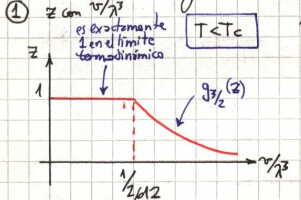
\includegraphics[scale=0.5]{images/1606329632.jpg}

Esto de arriba corresponde a $T < T_C $ para el caso $\lambda^3/v > 2.612 $ y se ve que 
$z = N_0/(N_0+1) \to 1$ si $N_0\to\infty$.

Cuando $v/\lambda^3$ es chico se saturan los $N_e$ y entonces $ z \to 1 $.

Cuando $v/\lambda^3$ es grande no hay condensado y entonces $ \lambda^3/v \approx z $ o bien
$ 1/ (v/\lambda^3) \approx z $.

Para la presión tendremos
\[
	\beta p = \frac{1}{\lambda^3} g_{5/2}(z)
\]
Otra observación es que $P_{BE}(T=0)=0$. Las partículas $N_e$ en la fase normal hacen presión que es la
mitad de la del gas ideal mientras que las de $N_0$ no hacen presión en absoluto.

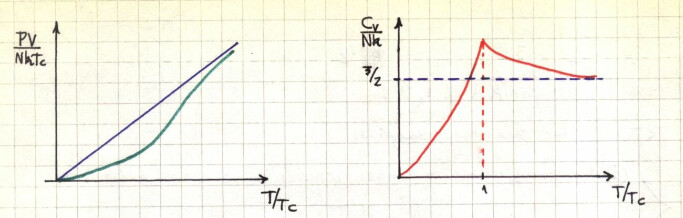
\includegraphics[scale=0.4]{images/1606329638.jpg}

con $ z = 1 ( T < T_c ) $
\[
	\frac{p}{kT} = \frac{(2\pi m k T)^{3/2}}{h^3} g_{5/2}(1) = 
	\frac{1}{ v (T_c/T)^{3/2} g_{3/2}(1) } g_{5/2}(1)
\]
\notamargen{Tenía anotado por allí $p \propto T^{5/2}$.}
\[
	p = 1.34 \frac{(2\pi m )^{3/2}}{h^3} (kT)^{5/2} \qquad \qquad 
	\frac{pV}{NkT} = 0.513 \Frac{T}{T_c}^{3/2}
\]
con $ z = 1 ( T = T_c ) $
\[
	\beta p = \frac{ g_{5/2}(1) }{ g_{3/2}(1) v } = \frac{0.513}{v}
\]
\[
	p = 0.513 \frac{NkT}{V} \qquad \text{ es aprox. $1/2 p$ gas ideal clásico }
\]
con $ z \lesssim 1 ( T > T_c ) $
\[
	\beta p = \frac{1}{v} \frac{ g_{5/2}(z) }{ g_{3/2}(z) }
\]
pero no podemos expandir en el virial porque $ \lambda^3 / v $ no es chico.

Con $ z \approx 0 \: ( T \gg T_C ) $
\[
	\beta p v = \frac{pV}{NkT} = \sum_{l=0}^\infty a_l \Frac{\lambda^3}{v}^{l-1}
\]
usando toda la serie y procediendo en modo análogo a Fermi se obtienen
\notamargen{ Los $a_\ell$ son los coeficientes del virial -que son los mismos
para Fermi-.}
\[
	\begin{cases}
	 a_1 = 1 \\
	 a_2 = -0.17678 \\
	 a_3 = -0.00330
	\end{cases}
\]
\[
	\frac{pV}{NkT} = 1 - 0.17678 \Frac{\lambda^3}{v} - 0.00330 \Frac{\lambda^3}{v}^2
\]

DIBUJO 

El virial vale en $\lambda^3/v \ll 1$ (alta $T$ y baja $N/V$ )

A bajas $T$ se comportan de modo muy diferente, $p_{\text{ Fermi }} > 0 $ y
$p_{\text{ Bose }} \approx 0$

\begin{ejemplo}{\bf Problema 2 -tip-}
Es $e_{p,n_i} = p^2/ 2m + n_i \varepsilon_1 $ donde $n_i=0,1$ y entonces es un grado de libertad interno.
 
\end{ejemplo}


% =================================================================================================
\subsection{Análisis del gas ideal de Bose}
% =================================================================================================

\begin{itemize}
 \item $ \lambda^3 / v \ll 1 $ y entonces $ z \ll 1 $ $\quad  [T \gg T_c ] $ (o sea $T$ alta y $N/V$ baja )
 tenemos un desarrollo del virial porque $z \ll 1$
 \[
	\frac{\beta p V}{N} = \sum_{l=1}^\infty a_l \Frac{\lambda^3}{v}^{l-1} = \frac{ g_{5/2}(z) }{ g_{3/2}(z) }
 \]
 \[
	\beta p V \approx 1 - \frac{\lambda^3}{v} \frac{1}{2^{5/2}} \qquad \qquad 
	U = \frac{3}{2}pV = \frac{3}{2} NkT \left( 1 - \frac{\lambda^3}{v} \frac{1}{2^{5/2}} \right)
 \]
 Como $a_2 < 0$ se tiene que la presión para Bose Einstein es menor a la presión clásica. Siguiendo
 podemos trabajar una expresión para el calor específico
 \[
	\frac{C_V}{kT} = \frac{3}{2} \left( 1 + 0.0884 \Frac{\lambda^3}{v} + 
	0.0066 \Frac{\lambda^3}{v}^2 + ... \right)
 \]
 
 \item $ \lambda^3 / v \approx 1 $ y entonces $ z < 1 $ $\quad  [T > T_c ] $
 \[
	\beta p V = \frac{ g_{5/2}(z) }{ g_{3/2}(z) }
 \]
 \item  $ \lambda^3 / v = 2.612 $ y entonces $ z = 1 $ $\quad  [T = T_c ] $
 \[
	\beta p V = \frac{ g_{5/2}(z) }{ g_{3/2}(z) } \approx \frac{1.34}{2.612} \approx 0.513
 \]
 \item $ \lambda^3 / v \gg 1 $ y entonces $ z = 1 $ $\quad  [T < T_c ] $ (baja temperatura $T$ y alta
 densidad $N/V$) y hay que considerar el  fundamental
 \[
	\beta p = \frac{1}{\lambda^3} g_{5/2}(1) \qquad \qquad \lambda^3\Frac{N-N_0}{V} = g_{3/2}(1)
 \]
 \notamargen{Con $z=1$ y $T<T_c$ expresamos todo en términos de $(T/T_c)$.}
 que lleva a 
 \[
	\left( 1 - \frac{N_0}{N} \right) = \Frac{T}{T_c}^{3/2}
 \]
 puesto que $T_c$ es tal que 
 \[
	\frac{h^3}{(2\pi m kT_c)^{3/2}} \frac{N}{V} = g_{3/2}(1) = \frac{\lambda^3}{v}\Frac{T}{T_c}^{3/2}
 \]
 \[
	\beta p V = \frac{ g_{5/2}(z) }{ g_{3/2}(z) } \Frac{T}{T_c}^{3/2} = 0.513 \Frac{T}{T_c}^{3/2}
 \]
 \[
	\frac{\lambda^3}{v} \Frac{T}{T_c}^{3/2} = g_{3/2}(1) \quad \Rightarrow \quad \frac{1}{\lambda^3} =
	\frac{1}{v}\Frac{T}{T_c}^{3/2} \frac{1}{g_{3/2}(1)}
 \]
\end{itemize}

Con el aumento de la temperatura aumentan ambos miembros en la ecuación 
\[
	\frac{\lambda^3}{v} = g_{3/2}(z)
\]
pero como $g_{3/2}$ está acotada esto lleva a la condensación de Bose.

Desde la expresión de la energía $ U = 3/2 p V $ y $C_V = \dpar{}{T}(3/2 p V)$
y entonces
\begin{itemize}
 \item $ T < T_c $ 
 \[
	C_V = \dpar{}{T}\left( \frac{3}{2} N k \Frac{T}{T_c}^{3/2} 0.513  \right) = 
	\frac{15}{4} N k \Frac{T}{T_c}^{3/2} 0.513 \qquad C_V \propto T^{3/2}
 \]
 \item $ T = T_c $ 
 \[
	C_V = N k \; 0.513 \frac{15}{4} = N k 1.92375
 \]
 \item $ T > T_c $ 
 \[
	C_V = \left( \frac{15}{4}\frac{ g_{5/2}(z) }{ g_{3/2}(z) } - 
	\frac{9}{4} \underbrace{\frac{ g_{3/2}(z) }{ g_{1/2}(z) }}_{\to \infty \text{ en } z=1} \right)
 \]
 $C_V$ es continuo.
 \item $ T \gg T_c $ 
 \[
	C_V = N k \frac{3}{2} \dpar{}{T} \left( T \sum_{l=1}^\infty a_l \Frac{\lambda^3}{v}^{l-1} \right)
 \]
 \[
	C_V = N k \frac{3}{2} \left( 1 + 0.0884 \Frac{\lambda^3}{v} + ... \right)
 \]
\end{itemize}

DIBUJO

Entonces tenemos dos fases macroscópicas, que dependen de la temperatura
\begin{itemize}
 \item Fase normal: consisten en las partículas de los niveles excitados,
 \[
	N_e = N \Frac{T}{T_C}^{3/2}
 \]
 \item Fase condensada
 \[
	\frac{N_0}{N} = 1 - \Frac{T}{T_C}^{3/2}
 \]
\end{itemize}

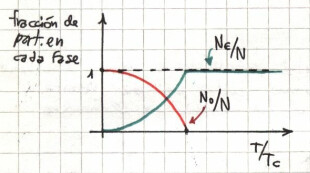
\includegraphics[scale=0.5]{images/1606329628.jpg}

Y vemos que $N_0 \to \infty$ en forma comparable a como $N \to \infty$. El $N_0$ macroscópicamente poblado
es la condensación.

\subsection{Condensado de Bose como transición de fase}

\[
	\frac{N_0}{N} = 1 - \Frac{T}{T_c}^{3/2}
\]
\[
	\frac{N_0}{N} = 1 - \frac{v}{v_c}
\]
que se obtiene desde las siguientes
\[
	\frac{\lambda^3(T_c)}{v} = g_{3/2}(1) \qquad \qquad  \frac{\lambda^3(T)}{v_c} = g_{3/2}(1)
\]
para llegar a la relación útil:
\[
	\Frac{T}{T_c}^{3/2} = \frac{v}{v_c}
\]
\notamargen{ $\lambda^3 = h^3/(2\pi m k T)^{3/2}$ y $\frac{\lambda^3}{v_c} = g_{3/2}(1) = \frac{\lambda^3}{v} 
\frac{v}{v_c}  $}

En $ \frac{\lambda^3}{v} \leq g_{3/2}(1) $ vale 
\[
	\frac{\lambda^3}{v} = g_{3/2}(z) \text{ no tengo en cuenta $N_0$ }
\]
\[
	\frac{v_c}{v} = \frac{ g_{3/2}(z) }{ g_{3/2}(1) } \quad \Rightarrow \quad 
	\Frac{T}{T_c}^{3/2} = \frac{ g_{3/2}(z) }{ g_{3/2}(1) } 
\]

Se vio que con $ V \to \infty $
\[
	\frac{1}{V} \log (1-z) \to 0 
\]
y entonces 
\[
	\beta p = \frac{1}{\lambda^3} g_{5/2}(z) \qquad v > v_c
\]
\[
	\beta p = \frac{1}{\lambda^3} g_{5/2}(1) \qquad v \leq v_c
\]
\[
	\beta p = \frac{ g_{5/2}(1) }{ v_c g_{3/2}(1) }
\]
es decir que la presión $p$ no depende del $v$

Con $v > v_c$ 
\[
	p = \frac{ k T g_{5/2}(z) }{\lambda^3} = \Frac{h^2}{ 2\pi m } \frac{1}{\lambda^3} g_{5/2}(z)
\]
que conlleva a 
\[
	kT = \Frac{h^2}{ 2\pi m } \frac{1}{\lambda^2} \qquad 
	p =  \Frac{h^2}{ 2\pi m } \frac{ g_{5/2}(z) }{ v^{5/3} [ g_{3/2}(z) ]^{5/3} }
\]
y con $v > v_c$ 
\[
	pv^{5/3} = \Frac{h^2}{ 2\pi m } \frac{ g_{5/2}(z) }{ [ g_{3/2}(z) ]^{5/3} }
\]
con $v \leq v_c$ 
\[
	p = \frac{ k T }{ v_c } \frac{ g_{5/2}(1) }{ g_{3/2}(1) }
\]

Vemos que en $ v = v_c $ es
\[
	pv^{5/3} = \Frac{h^2}{ 2\pi m } \frac{ g_{5/2}(1) }{ [ g_{3/2}(1) ]^{5/3} }
\]
\[
	p = \Frac{h^2}{ 2\pi m } \frac{ g_{5/2}(1) }{ v_c g_{3/2}(1) }\frac{1}{\lambda^2} =
	\frac{kT}{v_c}\frac{ g_{5/2}(1) }{ g_{3/2}(1) }
\]
y entonces se ve que es continua.

\begin{center}
\begin{tabular}{c|c}
 $\displaystyle \beta p = \frac{1}{\lambda^3} g_{5/2}(z) \quad v \geq v_c \quad $ & 
 $\displaystyle \quad \beta p = \frac{1}{\lambda^3} g_{5/2}(1) \quad v \leq v_c \quad $\\
 & \\
 $\displaystyle \frac{\lambda^3}{v} = g_{3/2}(z) \quad v > v_c \quad $ 
 & $\displaystyle \quad \frac{\lambda^3}{v} = g_{3/2}(1) \quad v = v_c \quad $
\end{tabular}
\end{center}

\begin{itemize}
 \item $ v \geq v_c $
 \[
	p = \frac{ kT }{v_c} g_{5/2}(z) = \frac{ ( 2 \pi m )^{3/2} }{ h^3 } ( kT )^{5/2} g_{5/2}(z)
 \]
 \[
	p = \Frac{h^2}{2\pi m}\frac{1}{\lambda^5}g_{5/2}(z) = 
	\Frac{h^2}{2\pi m} \frac{g_{5/2}(z)}{v_c^{5/3} [g_{3/2}(z)]^{5/3}}
 \]
 \[
	\boxed{ p v^{5/3} = \Frac{h^2}{2\pi m} \frac{g_{5/2}(z)}{ g_{3/2}(z)^{5/3}} }
 \]
 \item $ v \leq v_c$
 \[
	p = \frac{ kT }{v_c} g_{5/2}(1) = \boxed{ \Frac{kT}{v_c} \frac{g_{5/2}(1)}{g_{3/2}(1)} }
 \]
 
 Las isotermas del gas ideal de Bose serán algo como 
 
 DIBUJO
 
 Una dada $ T_1 $ determina un $v_{c_1}$ pués
 \[
	\frac{\lambda^3(T_1)}{v_{C_1}} = g_{3/2}(1) \quad \to \quad v_{C_1} = \frac{\lambda^3(T_1)}{g_{3/2}(1)} 
 \]
 y en la zona condensada $p$ no depende del $v$.
 
 \notamargen{ $ \lambda^3(T) \propto T^{-3/2} $ A medida que $T$ sube el $v_c$ es más pequeño.}
 
 Si ponemos todo en función de $T$ resulta 
 \[
	v \leq v_c \qquad p = \frac{ ( 2 \pi m )^{3/2} }{ h^3 } ( kT )^{5/2} g_{5/2}(1)
 \]
 \[
	\dtot{p}{T} =   \frac{5}{2} \frac{ ( 2 \pi m )^{3/2} }{ h^3 }  ( k )^{5/2} T^{3/2} g_{5/2}(1) =
	\frac{5}{2} \frac{k}{\lambda^3} g_{5/2}(1) = \frac{5}{2} \frac{k}{v_c} \frac{g_{5/2}(1)}{g_{3/2}(1)}
 \]
  
 DIBUJO 
 \[
	\dtot{ p }{ T } = \frac{ ( 5/2 ) k T g_{5/2}(1) }{T v_c g_{3/2}(1) } 
 \]
 pero Clapeyron era
 \[
	\dtot{ p }{ T } = \frac{ L }{ T \Delta V } \qquad \Rightarrow \qquad 
	\boxed{  \dtot{ p }{ T } = \frac{ ( 5/2 ) k T g_{5/2}(1) / g_{3/2}(1) }{T v_c} }
 \]
 
Es una transición de fase de primer orden 
 \notamargen{ $ \dtot{ p }{ T } = \frac{ L }{ T \Delta V } = \frac{ T \Delta S }{ T \Delta V } = 
 \frac{ \Delta S }{ \Delta V } $}
 \[
	S = \frac{U + pV - \mu N}{T} = \frac{ 5/2 pV - \mu N }{T}
 \]
 \[
	\frac{S}{kN} = \frac{5}{2} \frac{pV}{NkT} - \frac{\mu}{kT}
 \]
y entonces 
 \[
	T > T_c \qquad \qquad \frac{S}{kN} = \frac{5}{2} \frac{ g_{5/2}(z) }{ g_{3/2}(z) } - \log z
 \]
 \[
	T < T_c \qquad \qquad \frac{S}{kN} = \frac{5}{2} 0.513 \Frac{T}{T_c}^{3/2}
 \]
 \notamargen{$ \Frac{T_c}{T}^{3/2} = \frac{ \lambda^3 }{ g_{3/2}(1) v } $}
 \[
	\text{Con } T \to 0 \qquad \qquad \frac{S}{kN} \propto T^{3/2} 
 \]
y por lo tanto vale la tercer de la termodinámica.
Para $ T < T_c $ es
\[
	S = N k \frac{5}{2} \frac{ g_{5/2}(1) }{ g_{3/2}(1) } \Frac{v}{v_c} \quad \to \quad 
	\dpar{S}{V} = \frac{\partial S/N}{\partial V/N} = \dpar{s}{v}
\]
siendo $s$ entropía por unidad y $v$ volumen específico.
\[
	\dpar{s}{v} =  \frac{ ( 5/2 ) k g_{5/2}(1) / g_{3/2}(1) }{v_c} = \dtot{p}{T}
\]
y acá es donde vemos que es una transición de fase de primer orden.
\end{itemize}



% =================================================================================================
\section{Cuánticos IV --reubicar--}
% =================================================================================================

algunos temitas sueltos:

números de ocupación

gas de Fermi $p$ y $c_v$

gas de Fermi $p$ y $c_v$

Condensado de Bose

\notamargen{¿El condensado BE requiere población de los niveles o $V$ total de algún tipo?}

El coeficiente lineal del virial $ 1/ 2^{5/2} = 0.1767767 $ sale considerando las $ f_{\nu}(z) $ hasta orden
uno y tirando términos más allá.

\notamargen{Tenía unas consultas agarradas con clip: ¿porqué hay una cúspide en $C_v$? ¿transiciones?}

El requerimiento $ \mu < 0 $ viene de que el fundamental $ n_0 $ no puede tener población negativa
\[
	n_0 = \frac{1}{\euler^{\beta(e_0 - \mu)} -1} = \frac{1}{\euler^{-\beta\mu} -1} \geq 0
\]
\[
	\euler^{-\beta\mu} -1 > 0 \qquad \Rightarrow \quad \mu < 0
\]
Con $\mu \to 0^-$ tenemos $ n \to \infty $

En el caso del condensado establecemos desde 
\[
	\frac{\lambda^3(T)}{v} = g_{3/2}(1) 
\]
que lleva para $T_c$ (para $v$ fijo) o $v_c$ (para $T$ fija) versiones evaluadas de la anterior ecuación.

Para la población de los estados excitados
\[
	p_x = \frac{h}{V^{1/3}}n_x \Rightarrow  \vb{p} = \frac{h}{V^{1/3}} \vb{n}
\]
\[
	\frac{n_{e_i}}{V} = \frac{1}{V} \frac{1}{ z^{-1}\euler^{\beta e_i} - 1 } \leq 
	\frac{1}{V(\euler^{\beta e_i} - 1)} = \frac{1}{V(\sum_{l=1}^\infty (\beta e_i )^l/l!)}
\]
pués $z^{-1} = 1/z \leq 1$
\[
	\beta e = \frac{\beta p^2}{2m} = \frac{\beta}{2m} \frac{h^2}{V^{2/3}} ( n_x^2 + n_y^2 + n_z^2)
\]
\[
	\frac{2m}{V^{1/3} \beta h^2 (\sum_{l=1} ... )} \to 0 \quad \text{ si } \quad V \to \infty
\]
y entonces
\[
	\frac{n_e}{V} \to 0 \quad \text{ si } \quad V \to \infty
\]

Esto significa que si $V$ es muy grande, en el condensado se tenderá a que todas las partículas se hallen en
$ e = 0 $ pues 
\[
	\frac{N_e}{N} \to 0 \qquad \qquad \frac{N_0}{N} \to 1
\]

Véamoslo en la ecuación de $N$,
\[
	\frac{\lambda^3 N}{V} = g_{3/2}(1) + \frac{\lambda^3}{V} \frac{z}{1-z}
\]
y si $z \to 1$ de forma que $z/(1-z) \gg 1$ entonces $g_{3/2}(1)$ es despreciable de modo que
\[
	\frac{\lambda^3 N}{V} \approx \frac{\lambda^3}{V} \frac{z}{1-z} = \frac{\lambda^3 N_0}{V} 
\]
y se da que $ N \sim N_0 $.

En Bose se da $ 0 < z < 1$

DIBUJITOS

Con $ z \ll 1$ es $ \lambda^3 / v \approx z $ y entonces $ z \approx 1/ (v/\lambda^3) $.
Con $ z=1 $ es $ \lambda^3 / v = 2.612$n pero si $ \lambda^3 / v > 2.612 $ entonces $z$ no se mueve y
sigue en su valor 1.


\subsection{Cuánticos 5 - Cuánticos 5b --reubicar--}

presión gas de Bose

$C_V$ gas de Bose

El condensado de Bose es una transición de fase de primer orden.
Crece la población del fundamental de modo espectacular. El parámetro $ \lambda^3/V $ se encarga de
adjustar la población del fundamental.

límite clásico función de partición

cálculo de $ Tr (\euler^{-\beta A} ) = Q_N(V,T) $

diferencia con el caso clásico

potencial efectivo

\notamargen{Ver la transición de fase con el tema del calor latente. ¿Cómo era lo de Clayperon?}

Podemos comparar presión con el gas ideal para reconoder si es Fermi o Bose.

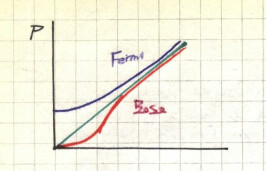
\includegraphics[scale=0.5]{images/1606329551.jpg}


El $C_V$ es continuo. Veamos que da
\[
	T<T_C \qquad \frac{C_V}{Nk} \propto T^{3/2}
\]
\[
	T=T_C \qquad \frac{C_V}{Nk} \approx 1.925 > \frac 3 2
\]
\[
	T>T_C \qquad \dpar{}{T}\left( \frac{3}{2} T \frac{g_{5/2}(z)}{g_{3/2}(z)} \right) \frac{C_V}{Nk} 
\]


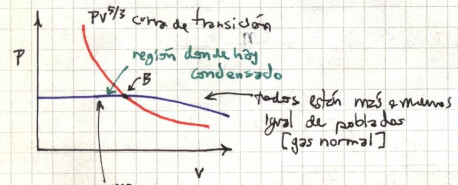
\includegraphics[scale=0.5]{images/1606329555.jpg}

La flecha de abajo señala una región de coexistencia. Entonces el fundamental se empieza a poblar mucho.
Cuando tengo todos en el condensado es $ S \to 0, T \to 0$ y se ve que satisface la tercer ley.
Los boltzmanniones no cumplen esto (no están pensados para satisfacer la tercer ley).

Tiene calor latente $ \Delta H $, entonces tenemos una transición de fase de primer orden.

\subsection{Límite clásico de la función de partición}

Cuando se overlapean las funciones de onda en las partículas hay que realizar las perturbaciones 
correspondientes.
El límite clásico es la no permutación. La simetría hace surgir términos efectivos de interacción
(atractivos o repulsivos)

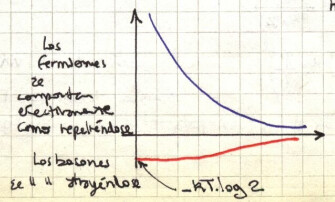
\includegraphics[scale=0.5]{images/1606329560.jpg}


\begin{ejemplo}{\bf Problema 5}

Se tiene lo siguiente:
\[
	\frac{m}{2}( \omega_x^2 x^2 + \omega_y^2 y^2 + \omega_z^2 z^2 )
\]
es decir un planteamiento semiclásico, de manera que considero un continuo.

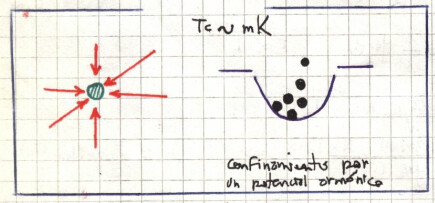
\includegraphics[scale=0.3]{images/1606329642.jpg}

Primero se considera el caso 1D, entonces es
\[
	E = \frac{m}{2} \omega^2 x^2 + \frac{ p^2 }{2m}
\]
y hago la conversión al continuo según
\[
	\sum_\text{estados} \longrightarrow \frac{1}{h} \int dx dp \longrightarrow \int g(e) de
\]

Con el cambio de variables $ R^2 = X^2 + Y^2 $ se tienen
\[
	dx = \sqrt{2/(m\omega^2)} dX \qquad dp = \sqrt{2m} dY
\]
de modo que $ dX dY = 2 \pi R dR = \pi de $ y como 
\[
	\frac{1}{\hbar} dx dp = \frac{1}{\hbar\omega} de
\]
se ve que $ g(e) = 1 / (\hbar \omega )$. Hemos hallado un $g(e)$ constante, lo cual parece razonable 
porque es el espaciado entre niveles de energía para el oscilador armónico en el caso cuántico.
Entonces este enfoque semiclásico lleva al mismo resultado,
\[
	\Delta E = \hbar \omega \qquad H = \left( n + \frac{1}{2} \right) \hbar \omega \qquad 
	g(e) = \frac{\text{\# de estados}}{\text{unidad de energía}}
\]

Vayamos ahora al caso 3D
\[
	E = \frac{m \omega^2 }{ 2 }( x_1^2 + x_2^2 + x_3^2 ) + \frac{1}{2m} ( p_1^2 + p_2^2 + p_3^2 )
\]
y como $ R^2 = x_1^2 + x_2^2 + x_3^2 + y_1^2 + y_2^2 + y_3^2 $ que es el módulo al cuadrado de un
vector en $\mathbb{R}^6$. De tal suerte es
\[
	\frac{ d^3x d^3p }{ h^3 } = \frac{ 2^3 }{ h^3 \omega^3 } d^3X d^3Y = \frac{ R^5 dR }{ (\hbar \omega)^3}
\]
donde $d^3X d^3Y = \pi^3 R^5 dR $ y el volumen $\Theta_{6D} = \pi^3 R^6/6$ de tal manera que
\[
	g(e) = \frac{1}{2(\hbar\omega)^3} e^2 de
\]

Ahora, en 3D, $g(e)$ sí depende de la energía. El número de estados va de $g_{xp} d^3x d^3p$ a $g_e de$.
No interesa ver el límite termodinámico, $N\to\infty, V\to\infty$ con $N/V$ finito.
En el problema del oscilador armónico $ N/\omega^3 $ será el límite termodinámico.
Si $\hbar \omega \ll k T$ entonces lo puedo considerar un continuo. $kT_c \sim 20-200 \hbar\omega$, este
es el caso en condensación de Bose

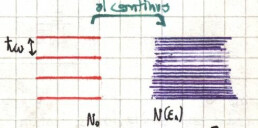
\includegraphics[scale=0.4]{images/1606329650.jpg}

\[
	N = \sum_e \frac{ z \euler^{-\beta e} }{ 1 - z \euler^{-\beta e}} \longrightarrow
	\int_0^\infty \frac{ g(e) de }{ z^{-1}\euler^{\beta e} - 1} + \frac{z}{1-z} 
	+ \frac{ z \euler^{-\beta e_1} }{ 1 - z \euler^{-\beta e_1}} 
\]
donde separo la contribución de finitos términos lo cual no debería joder. La primer integral es,
mediante el cambio de variables $\beta e = x$
\[
	I = \frac{ 1 }{ 2 ( \hbar \omega )^3 } \int_0^\infty \frac{1}{\beta} \frac{ x^2 dx }{ z^{-1} \euler^x - 1}
\]
relacionados con la expresión de $g_\nu$ (que tendría que estar en un apéndice al final).
Importante remark: notemos que con $\nu> 1$ con $z\to$ converge pero con $\nu=1$ (lo cual tiene que
ver con la dispersión y la dimensión del problema) con $z\to 1$ diverge.
\[
	N = \frac{z}{1-z} + \Frac{kT}{\hbar\omega}^3 g_3(z) + 
	 \frac{ z \euler^{-\beta e_1} }{ 1 - z \euler^{-\beta e_1}} 
\]
\[
	N \omega^3 \Frac{ \hbar }{ kT }^3 = 
	\Frac{ \omega \hbar }{ kT }^3 \frac{ z }{ 1 - z } + g_z(z) + 
	\Frac{ \omega \hbar }{ kT }^3 \frac{ z \euler^{-\beta e_1} }{ 1 - z \euler^{-\beta e_1}} 
\]
donde $g_3(z)$ es creciente pero como $z\leq 1$ está acotada. El primer término permanece macroscópicamente
poblado en el límite termodinámico. El último término en cambio es aproximadamente nulo en dicho límite.

\includegraphics[scale=0.4]{images/1606329656.jpg}

Puedo despejar una $T_c$

\includegraphics[scale=0.4]{images/1606329660.jpg}

Para la $T_c$ sería
\[
	N \Frac{ \omega \hbar }{ kT } = g_3(z=1)
\]
de manera que 
\[
	N = N_0 + \Frac{ kT }{ \omega \hbar }g_3(z\neq 1)
\]
y para $T < T_c$ es 
\[
	N = N_0 + N \Frac{T}{T_c}^3 \qquad  \frac{N_0}{N} = 1 - \Frac{T}{T_c}^3
\]

\includegraphics[scale=0.4]{images/1606329664.jpg}

La energía será
\[
	E = \int_0^\infty \frac{ g(e) de }{ z^{-1} \euler^{\beta e} - 1} = 
	3 \frac{( k T )^4}{( \hbar \omega )^3} g_4(z)
\]
Con $N_0 \ll N $ es 
\[
	 N \sim \Frac{ kT_c }{ \omega \hbar }g_3(1)
\]
y finalmente
\[
	\frac{ E }{ N k T_c } = \frac{3 g_4(1)}{g_3(1)} \Frac{T}{T_c}^4.
\]

\end{ejemplo}



\begin{ejemplo}{\bf Problema 6}

Relacionado con excitaciones en un sólido.

\includegraphics[scale=0.4]{images/1606329667.jpg}

Entonces,
\[
	E_{\text{cin}} = \frac{1}{2} m \sum_{i=1}^{3N} \dot{x}^2_i
\]
\[
	E_{\text{pot}} = \phi_0 + 
	\frac{1}{2} \sum_{ij} \left. \dparcru{ \phi}{x_i}{x_j}\right|_{x_{i0},x_{j0}}
	(x_i-x_i^0)^2(x_j-x_j^0)^2 + ... 
\]
Pero podemos cambiar de coordenadas
\[
	H = \phi_0 + \sum_{i=1}^{3N} \frac{1}{2} ( m \dot{q}^2_i + \omega^2_i q_i^2 ),
\]
donde $\{ q_i \}$ son los modos normales. Un modo normal es un oscilador armónico.
Clásicamente tenemos los modos normales $\vb{e} \euler^{ i ( \vb{k}\cdot \vbx - \omega t)} $ donde estos 
son vectores de polarización y $\vb{k}$  es el vector de propagación y  $\vb{e}$ el vector de polarización.

Cuánticamente hablamos de fonones, que serán cuantos de excitación de cada modo normal.
El número de fonones es análogo al formalismo de los números de ocupación.
Los fonones se pueden crear y destruir sin invertir energía de manera que $\mu=0$ pero aún utilizo la
estadística de Bose.
Podemos considerar dos aproximaciones.
\begin{itemize}
 \item Aproximación de Einstein: $\omega_i = \omega$ constante para todo $i$.
 \item Aproximación de Debye: El sólido es un medio elástico, continuo y deformable, el espectro de
 $\omega$ va al continuo.
\end{itemize}

\includegraphics[scale=0.4]{images/1606337002.jpg}

Quiero usar Debye. En 3D asumo dispersión como $ \omega = c k $  y entonces se tiene
\[
	g(\omega) d\omega = \frac{3V}{\hbar^3} 4 \pi p^2 \: dp = \frac{3V}{(2\pi)^3} 4 \pi k^2 \: dk
\]
donde $ \vb{p} = \hbar \vb{k} $ o bien integrando y considerando relación $ \omega c = k $,
\[
	3N = \int_0^{\omega_D} d(u) \: du = \int_0^{\omega_D} \frac{V \omega^2 }{2 \pi^2 c^3} \: d\omega
\]
desde la cual despejamos la frecuencia de corte
\[
	\omega_D = \Frac{ 6 \pi^2 }{ v}^{1/3}
\]
que se puede escribir también en términos de una longitud de onda de corte como
\[
	\omega_D = \frac{ 2 \pi }{\lambda_D} c \qquad  \lambda_D = \Frac{ 4 \pi v }{3}^{1/3}.
\]

La integral da $3N$ y entonces se define una $ \omega $ de corte. Claramente la $\omega$ no puede
implicar desplazamientos mayores a la distancia interparticular.

En el caso de $ D $ dimensiones se tiene $ \omega = \alpha |\vb{k}|^s$ y el número de estados entre
$p, p +dp$ da algo como
\[
	g \frac{L^D}{h^D} d^Dp
\]
donde $g$ es por la polarización, y el $L$ es la discretización por las condiciones de contorno periódicas.
Es
\[
	g \frac{ L^D }{ (2\pi)^D } A k^{D-1} \: dk
\]
que es la integral sobre la parte angular que en $D=3$ es $A=4\pi$ y en $D=2$ es $A=2\pi$.
Con esto se puede arribar a
\[
	g(\omega) d\omega = g \frac{ L^D }{ (2\pi)^D } A \frac{1}{S \alpha^{D/s}} \omega^{(D-s)/s} \: d\omega,
\]
pero esto deber cortarse en
\[
	DN = \int_0^{\omega_D} g(\omega) \: d\omega.
\]

\end{ejemplo}





% \bibliographystyle{CBFT-apa-good}	% (uses file "apa-good.bst")
% \bibliography{CBFT.Referencias} % La base de datos bibliográfica

\end{document}

	
		\documentclass[10pt,oneside]{CBFT_book}
	% Algunos paquetes
	\usepackage{amssymb}
	\usepackage{amsmath}
	\usepackage{graphicx}
% 	\usepackage{libertine}
% 	\usepackage[bold-style=TeX]{unicode-math}
	\usepackage{lipsum}

	\usepackage{natbib}
	\setcitestyle{square}

	\usepackage{polyglossia}
	\setdefaultlanguage{spanish}
	



	\usepackage{CBFT.estilo} % Cargo la hoja de estilo

	% Tipografías
	% \setromanfont[Mapping=tex-text]{Linux Libertine O}
	% \setsansfont[Mapping=tex-text]{DejaVu Sans}
	% \setmonofont[Mapping=tex-text]{DejaVu Sans Mono}

	%===================================================================
	%	DOCUMENTO PROPIAMENTE DICHO
	%===================================================================

\begin{document}

% =================================================================================================
\chapter{Elementos de la teoría de fenómenos críticos}
% =================================================================================================


% =================================================================================================
\section{Ising 1}
% =================================================================================================

El modelo de Ising intenta explicar el ferromagnetismo. El estado espontáneo es spines desordenados
(no hay magnetización). Considero solo interacciones entre primeros vecinos.
Si cambio todo un bloque a lo sumo solo hay un cambio en la frontera, porque las interacciones son
entre primeros vecinos.

El proceso de ``generar paredes'' minimiza el $A$ y desordena y aumenta la $S$ de manera que el sistema
evoluciona así. Este es el modelo de Ising en 1D. En 2D se complica sobremanera.
La cantidad $\chi(b,i)$ camina sobre todos los dominios en una sola configuración.
Hay regiones donde se da la magnetización espontánea en Ising 2D.


\begin{itemize}
 \item Modelo sencillo de sistema interactuante
 \item Magnetización espontánea 1D y 2D:
 \subitem En 1D no hay magnetización espontánea
 \subitem En 2D hay magnetización espontánea
\end{itemize}

Fase es una porción de materia física y químicamente homogénea (asociada a la densidad atómica o molecular
uniforme) que no puede separarse por medios mecánicos.

Una fase puede ser una única sustancia o una mezcla.

El concepto de fase está también relacionado con el pasaje de la materia de una a otra fase.

\notamargen{corregir}

Estados de agregación (en función de la proximidad de sus componentes). Agua y aceite (líquido) es un sistema de dos 
fases.

La materia puede encontrarse en gran variedad de fases; las más conocidas están relacionadas con los estados de 
agregación. Pero dentro del estado sólido tenemos fases dependiendo de cómo sea la estructura interna.

Tenemos también sistemas que manifiestan fases ordenadas y desordenadas; aleaciones de sólidos, superconductividad.

Transición de fase: cuando una propiedad del sistema cambia discontinuamente frente a la variación de un parámetro 
intensivo ($T, p$ campo magnético).

\[
	\text{ interacciones entre partículas } \; \longrightarrow \; \text{ CORRELACIÓN A GRAN ESCALA }  
\]

Las transiciones de fase emergen de la interacción. Uno de los modelos más sencillos fuera del gas ideal es el modelo de
Ising (red con interacción entre primeros vecinos)
\[
	\boxed{ E_\nu = -H \sum_{i=1}^N (\mu S_i) - J \sum_{\braket{i,j}} S_i \cdot S_j }
	\label{energia_ising}
\]
\notamargen{Ising es energía dada por \eqref{energia_ising} e interacción a primeros vecinos.}

dibujo 


donde $\nu$ es una dada configuración de la red (valores $S_i$ con $i=1,2,...,N$)
\[
	S_i = \pm 1 \qquad \rightarrow \qquad \pm \mu S_i \text{ Momento magnético del spin i-ésimo }
\]
donde $\mu>0$, $J$ es constante de acoplamiento y $\sum_{<i,j>}$ se extiende sobre los pares de vecinos (primeros).

Con $J>0$ es favorable que todos los spines se hallen alineados. Entonces esto llevará a la magnetización espontánea: 
fenómeno de cooperación; la mayoría de los spines se orienta en una dirección y dan un valor de magnetización 
$\braket{M} \neq 0$
\[
	M_\nu = \sum_{i=1}^N \mu \cdot S_i^\nu
	\text{ (Magnetización) }
\]
\notamargen{$J>0$ ferromagnetismo y $J<0$ paramagnetismo}

Si los spines están orientados al azar, entonces habrá igual cantidad de $+1$ que de $-1$ y entonces
\[
	M \approx 0
\]

Si $H=0$ entonces $M$ es la magnetización espontánea.
\notamargen{$M$ se define como un momento dipolar magnético por unidad de volumen.}

Habrá magnetización con $T$ baja (o $J$ alto) y hasta una $T_\text{curie}$
\[
	Q_N(H,T) = \sum_{s_1=-1}^{+1} \; \sum_{s_2=-1}^{+1} \; ... \sum_{s_N=-1}^{+1} \;
	\euler^{ +\beta H \mu \sum_i^N S_i + \beta J \sum_{\braket{i,j}} S_i \cdot S_j }
\]
donde las sumatorias toman para cada $i$ los valores $S_i = +1, -1$
\[
	A = -kT\log Q \qquad \braket{E} = -\dpar{}{\beta}\log Q = kT^2 \dpar{}{T} \log Q
\]

Me interesa definir densidades de $ N_+, N_{++} $

\includegraphics[scale=0.4]{images/1606337009.jpg}

y consideraremos un efecto promedio
\[
	\frac{ N_{++} }{ N y/2 } = \Frac{ N_{+} }{ N }^2
\]
que es una aproximación de campo medio, definiendo un $L$ tengo muchos $\{ S_i \}$.
Al eliminar $\sigma$ perdemos la estructura fina de la red y hacemos estadística allí.

El campo magnético rompe la degeneración pues dessimetriza. Luego con $ H \to 0 $ y me quedo
con la curva que resultó no simétrica (el $A$ deja de ser simétrico).

\includegraphics[scale=0.4]{images/1606337012.jpg}

Esto es la aproximación de Bragg-Williams, que ha descartado las correlaciones; entonces
hemos contado nodos.
La aproximación de Bethe-Peierls tomo como unidades fundamentales

\includegraphics[scale=0.4]{images/1606337015.jpg}

$P(+,n)$ es la probabilidad condicional de tener un $+$ en el nodo central mientras que
$P(-,n)$ es la de tener un $-$ en el nodo central.
Otra apromicaicón
\[
	\frac{ N_{++} }{ N y/2 } = \frac{1}{2}( \sigma + 1 )
\]

El efecto del resto del sistema es una $ z = \euler^{\beta \mu} $ asociado a la influencia
del resto del sistema.

\[
	\sum_{n=0}^\gamma \: P(+,n)
\]
y sumo sobre todos los posibles vecinos hasta $\gamma$.

\includegraphics[scale=0.4]{images/1606337019.jpg}

Las fluctuaciones de la energía del sistema nos darán el calor específico $C_V$ (como en el $Z_{GC}$).
Se puede pensar como una transición del orden al desorden. En 2D tenemos magnetización espontánea.

\begin{ejemplo}{(Ejercicio 5.1 Chandler)}
\[
	E_0 = -J \sum_{\braket{i,j}} S_i \cdot S_j = -J  \sum_i^N \sum_j^\gamma \frac{S_i S_j}{2}
\]
para cada $i$ sumo en sus $\gamma$ vecinos el $j$ (sobre 2 para no contar dos veces).
\[
	E_0 = -J \sum_i^N \frac{S_i\gamma}{2} = -J N\frac{\gamma}{2} = -JND
\]
donde $D$ es la dimensionalidad.
\end{ejemplo}


Como es
\[
	E_\nu =  -H \sum_{i=1}^N \mu \cdot S_i - J \sum_{\braket{i,j}} S_i \cdot S_j \qquad
	\text{ y } \qquad \braket{M} = \braket{ \sum_i^N \mu \cdot S_i }
\]
entonces
\[
	\braket{M} = \braket{ \sum_i^N \mu \cdot S_i } = 
	\frac{ \sum_{s_1} \; \sum_{s_2} \; ... \sum_{s_N} \;
	\euler^{ \beta H \mu \sum_i^N S_i + \beta J \sum_{\braket{i,j}} S_i \cdot S_j } }{Q_N}
\]
\[
	\braket{M} = \frac{ \sum_{s_1} \; \sum_{s_2} \; ... \sum_{s_N} \;
	\dpar{}{\beta H} \left[ \euler^{ \beta H \mu \sum_i^N S_i + \beta J \sum_{\braket{i,j}} S_i \cdot S_j } 
	\right]}{Q_N} = \frac{\dpar{}{\beta H}(Q_N)}{Q_N}
\]
\[
	\braket{M} = \dpar{}{\beta H}\left( \log Q_N \right) = \dpar{}{\beta H}\left( -\beta A \right) =
	\dpar{}{H}\left( A \right)
\]

\subsection{No hay magnetización espontánea en 1D}

\notamargen{Error en Huang (14.6); es $-\dpar{}{H}(A_I)$}

DIBUJO 

Con $H=0$ invierto spines detrás de una pared.
\[
	E_0 = -J(N-1) \qquad E_f = -J[(N-1)-2p]
\]
\notamargen{$p$ es el número de paredes}

Varían los términos asociados a la pared
\[
	\Delta E = E_f - E_0 = 2Jp > 0
\]
con $p=1$ es $\Delta E = 2J$ y con $p=2$ es $\Delta E = 4J$ (es 2 por pared puesto que desaparece un $+$ y aparece
en su lugar un $-$).

La variación de $S$ está asociada con el número de formas de ubicar la pared
\[
	S = l \log (N-1)
\]
y es la $S$ del estado con una pared, el desordenado.
\[
	\Delta S = k \log(N-1)	\qquad (S_0 \equiv 0)
\]
que define al estado sin pared como de entropía $S_0=0$
\[
	A = U - TS \quad \rightarrow \quad \delta A = \delta U - T \delta S
\]
\[
	\delta J - kT \log(N-1)
\]
\notamargen{Para $p$ paredes es 
$\Delta A = 2Jp - kT \log [(N-1)(N-2)...(N-p)]$}

Con $T > 0$ tenemos que si desordeno (agrego paredes) sube $U$ y sube $S$.
En general, como 
\[
	\frac{\delta A}{kT} = \frac{2J}{kT} - \log(N-1)
\]
vemos que para $N\to\infty$ $\delta A < 0$ a menos de que $J/kT$ sea muy grande.

\notamargen{$S$ domina la minimización de $A$.}

En un sistema macroscópico 1D el desorden baja la $A$, entonces el equilibrio tiende
al desorden (no al orden).

Es decir, un sistema 1D de spines a $ T \neq 0 $ espontáneamente irá hacia $ A $
mínimas (mayor aleatoriedad), no se tiende a alcanzar estados ordenados.

\subsection{Magnetización espontánea en 2D}

La magnetización media por spín es
\[
	\mathcal{M} = \frac{1}{2} \Frac{N_+ - N_-}{N}
\]
Con $N\to\infty$ claramente será 0 a no ser que exista una preferencia por cierta dirección $+$ o $-$.

Queremos calcular todas las configuraciones posibles de un arreglo 2D de spines.
Para ello sistematizamos una dada construcción en dominios $\Box$ que engloban spines ($-$) y están
limitados por paredes.

DIBUJO ising


Los spines $+$ son una condición de contorno que con $N\to\infty$ es una perturbación que rompe la
simetría. También sirven para cerrar los dominios.

Cada dominio tiene una longitud $b$ medido en paredes $|$ y una dirección de recorrido de forma que 
los spines $-$ están siempre a la izquierda de la pared.
El tamaño de la red es $\sqrt{N} \times \sqrt{N} = N$. El área se mide en términos del dominio 
mínimo ``$\Box$''
\[
	\text{ dominio } = (b,i)
\]
donde $b$ es el número de paredes e $i$ una etiqueta.

A un mismo número de paredes según forma y localización tendrá varios dominios.

Una dada configuración del sistema tendrá ciertos dominios $(b,i)$

\begin{center}
\begin{tabular}{llll}
 & $b$ (paredes) & Areas (spines) & $b^2/16$ \\
\hline
 & 4 & 1 & 1\\
 & 6 & 2 & 2.25\\
 & 8 & 3,4 & 4
\end{tabular}
\end{center}

Si cada spin ocupa un área de 1, en términos de paredes el área que engloba un dominio de $b$ paredes
es 
\[
	\text{ Área dominio } \neq \frac{b^2}{16} \qquad \rightarrow \qquad S([b,i]) = \text{ Área dominio}
\]
\notamargen{Tengo una figura de longitud $b$ y si la quiero llevar a un cuadrado con suerte el lado
será $b/4$ de modo que su área es $b^2/16$}

Definimos ahora 
\[
	\chi([b,i]) = \begin{cases}
	              1 \qquad \text{ Si (b,i) ocurre en una dada configuración } \\
	              0 \qquad \text{ En caso contrario}
	             \end{cases}
\]
y $m(b)$ número de dominios de $b$ paredes.

Luego;
\[
	\boxed{ N_- = \sum_b \sum_i^{m(b)} \chi([b,i]) S([b,i]) } \quad [1]
\]
en el caso dibujado sería
\[
	N_- = 1 \cdot S(6,i) + 1 \cdot S(8,i') + 1 \cdot S(26,i'') \qquad 
	N_- = 1 \cdot  2 + 1 \cdot  4 + 1 \cdot 12 = 18
\]

Por la [1] se puede acotar, empezando por $m(b)$. Para ver el número de dominios de longitud $b$ piénsese que 
para la primera pared tengo $N$ posibilidades; para las siguientes $b-1$ tengo tres opciones pues no puedo volver,
y entonces 
\[
	m(b) \leq N 3^{b-1}
\]

Nótese que estamos considerando paredes abiertas y cerradas.

Luego,
\[
	\braket{N_-} \leq \sum_b \sum_i^{N3^{b-1}} \chi([b,i]) \underbrace{S([b,i])}_{\leq b^2/16}
\]
\[
	N_- \leq \sum_b \frac{b^2}{16} \sum_i^{N3^{b-1}} \chi([b,i])
\]
\[
	\braket{N_-} \leq \sum_b \frac{b^2}{16} \sum_i^{N3^{b-1}} \braket{\chi([b,i])}
\]

Pero
\[
	\braket{\chi([b,i])} = \frac{ \sum_{\{Si\}}' \euler^{-\beta E_{\{Si\}}} }
	{ \sum_{\{Si\}} \euler^{-\beta E_{\{Si\}}} }
\]
donde la sumatoria es en aquellas configuraciones que contienen al dominio $(b,i)$.

\notamargen{num: de todas las configuraciones posibles aquellas en las cuales se da el dominio $(b,i)$.
den: todas las configuraciones posibles.}

Removemos términos del denominador para acotar: pensamos que si en una dada configuración $C$ con $\{b,i\}$ revertimos 
en el dominio $\{b,i\}$ los spines llegamos a una configuración $\tilde{C}$
\[
	E_C - E_{\tilde{C}} = 2 \varepsilon b
\]

Al revertir los spines de un dominio pasamos a una configuración más ordenadas y por ende de menor energía
 
 DIBUJO
 
\[
	\frac{ \sum_{\{Si\}}' \euler^{-\beta E_{\{Si\}}} }{ \sum_{\{Si\}} \euler^{-\beta E_{\{Si\}}} }
	\leq 
	\frac{ \sum_{\{C\}} \euler^{-\beta E_C} }{ \sum_{\{C'\}} \euler^{-\beta E_{\tilde{C}}} } =
	\frac{ \sum_{\{C\}} \euler^{-\beta E_C} }{ \sum_{\{C\}} \euler^{-\beta E_{\tilde{C}}} 
	\euler^{2\beta\varepsilon b} } = \euler^{-2\beta \varepsilon b}
\] 
\[
	\braket{N_-} \leq \sum_b \frac{b^2}{16} \euler^{-2\beta \varepsilon b} N 3^{b-1} =
	\frac{N}{48} \sum_b b^2 [ 3 \euler^{-2\beta \varepsilon } ]^b
\]
\[
	\braket{N_-} \leq \frac{N}{48} \sum_{b=4,6,8,...} b^2 x^2,
\]
con $ x \equiv 3 \euler^{-2\beta \varepsilon } $

\[
	\braket{N_-} \leq \frac{N}{48} (16x^4 + 36x^6 + 64x^8 + ...) 
\]
Sea $b=2n$, entonces
\[
	\braket{N_-} \leq \frac{N}{48} \sum_{n=2,3,4,...} 4 n^2 (x^2)^n,
\]
con $x^2 = 9 \euler^{-4\beta\varepsilon} $
\[
	\braket{N_-} \leq \frac{N}{12} \sum_{n=2}^\infty n^2 r^n,
\]
con $r=9 \euler^{-4\beta\varepsilon}$
\[
	\braket{N_-} \leq \frac{N}{3} \frac{r^2}{(1-r)^3} \left[ 1 - \frac{3}{4}r + \frac{1}{4}r^2 \right]
\]
y esta cantidad para algún $\beta$ grande pero finito es menor a $N/2$.


% =================================================================================================
\section{Ising 2}
% =================================================================================================

La energía se podía escribir como
\[
	E_\nu = - H \sum_i^N (\mu s_i) - J \sum_{\braket{i,j}} s_i \cdot s_j 
\]

El grado de un nodo es $\gamma$ que depende de la red y de la dimensión,
\begin{center}
\begin{tabular}{lll}
2D & cuadrada & $\gamma=4$ \\
3D & SC & $\gamma=6$ \\
3D & BCC & $\gamma=8$
\end{tabular}
\end{center}

\notamargen{$\gamma$ es el número de vecinos. De cada nodo salen $\gamma$ líneas.}

\[ 
	\sum_{\braket{i,j}} = \frac{\gamma N}{2} = \text{ nro total de líneas } 
\]

dibujos

Tomando un nodo y trazando líneas a sus $\gamma$ vecinos tengo $ \gamma N/2 $ líneas dibujadas
(se divide en 2 por el doble conteo).

Tomando cada $\oplus$ trazo líneas a sus vecinos y defino
\[ 
	N_+ = \text{ nro de spines $\uparrow$} \qquad N_- = \text{ nro de spines $\downarrow$}
\]
\[ 
	N_{++} = \text{ nro de pares $\uparrow\uparrow$} \qquad 
	N_{--} = \text{ nro de pares $\downarrow\downarrow$}
\]
\[ 
	N_{+-} = \text{ nro de pares $\uparrow\downarrow$ o ($\downarrow\uparrow$)}
\]
\begin{itemize}
 \item 1) $ \gamma N_+ = 2N_{++} + N_{+-} $
 \item 2) $ \gamma N_- = 2N_{--} + N_{+-} $
 \item 3) $ N_+ + N_- = N $
\end{itemize}

\[
	\gamma N = 2N_{++} + 2N_{--} + 2N_{+-}
\]
\[
	\gamma N_+ + \gamma N_- = (2N_{++} + N_{+-}) + (2N_{--} + N_{+-})
\]
\[
	\frac{\gamma N}{2} = N_{++} + N_{--} + N_{+-} 
\]

Podemos poner todo en términos de $N_{++}, N_+, N$ y entonces
\[
	N_{+-} = \gamma N_+ - 2N_{++} \qquad N_- = N - N_+
\]
\[
	N_{--} = \frac{\gamma}{2}(N-N_+) - \frac{1}{2}(\gamma N_+ - 2N_{++}) =
	\frac{\gamma}{2} N - \gamma N_+ + N_{++}
\]
\begin{multline*}
	\sum_{\braket{i,j}} s_i \cdot s_j = N_{++} + N_{--} - N_{+-} =
	N_{++} + \frac{\gamma}{2}N - \gamma N_+ + N_{++} - \gamma N_+ + 2N_{++}= \\
	4N_{++} - 2\gamma N_+ + \frac{\gamma}{2}N 
\end{multline*}
\[
	s_i = N_+ - N_- = N_+ - (N-N_+) = 2N_+ - N
\]

La energía se puede escribir en función de estas variables
\[
	E_I = - H\mu (2N_+ - N) - J(4N_{++} - 2\gamma N_+ + \frac{\gamma}{2}N)
\]
\[
	E_I = -4JN_{++} - 2(H\mu - \gamma J)N_+ - \left( \frac{\gamma J}{2}- H\mu \right)N
\]

\notamargen{La energía depende de las cantidades $N,N_+,N_{++}$ y no del detalle de la distribución
de los mismos.}

La función canónica será
\[
	Q_I = \sum_{E_I} \euler^{-\beta E_I} = \euler^{\beta(J\gamma/2 - H\mu)N } \sum_{N_+=0}^N
	\left( \euler^{2\beta( \mu H - J\gamma )N_+ } \sum_{N_{++}}' \euler^{4\beta J N_{++}}
	\: g(N_+,N_{++})\right)
\]
donde $g(N_+,N_{++})$ es el número de configuraciones de $N_{++}$ y $N_{+}$ y la sumatoria primada se hace 
sobre los valores de $N_{++}$ consistentes con que hay $N_{+}$ spines up.

Esta expresión no ha sido resuelta salvo en 2D.

\subsection{Aproximación de Bragg-Williams}

\[
	\frac{N_+}{N} = \text{ (promedio) $\leftarrow$ correlaciones de largo rango } 
\]
\[
	\frac{N_{++}}{\gamma/2 N} = \text{  $\leftarrow$ correlaciones de corto rango } 
\]
y entonces $N_{+}/N$ está asociado a una visión global del sistema (un cuerpo), 
mientras que $N_{++}/(\gamma/2 N)$ lo está a una visión local del sistema (dos cuerpos).

Si un dado spin es $\oplus$ entonces tiene en promedio $N_{++}/(\gamma/2 N)$ vecinos del tipo $\oplus$.

Definimos unos parámetros de orden $L$ y $\sigma$
\[
	\frac{N_+}{N} = \frac{1}{2}(L+1) \qquad (\text{ todo } \downarrow) -1 \leq L \leq 1 (\text{ todo } \uparrow)
\]
\[
	\frac{N_{++}}{\gamma/2 N} = \frac{1}{2}(\sigma + 1) \qquad -1 \leq \sigma \leq 1
\]
\notamargen{Estamos viendo todo del lado de los spines $\oplus$.}
pero 
\[
	\sum_i s_i = 2N_+ - N = (L+1)N - N = NL,
\]
\[
	\braket{M} = \braket{ \sum_i^N \mu s_i } = \mu \braket{ \sum_i^N s_i } = \mu N \braket{L} 
\]
\[
	\frac{\braket{M}}{\mu N} \equiv \mathcal{M} = \braket{L}
\]
que es la magnetización por partícula (adimensional).
\[
	\sum_{\braket{i,j}} = \frac{1}{2} N \gamma (2\sigma - 2L + 1) 
\]

La energía es 
\[
	E = - H \mu \sum_i^N s_i - J \sum_{\braket{i,j}} =
	-H\mu NL - \frac{J}{2} N \gamma (2\sigma - 2L + 1) 
\]
y por partícula,
\[
	\epsilon \equiv \frac{E}{N} = -H\mu L - \frac{J}{2} \gamma (2\sigma - 2L + 1) 
\]

Hasta aquí el planteo es exacto; Bragg-Williams hace la aproximación
\notamargen{Significa que no hay correlaciones de orden corto salvo las que surgen
del orden largo. Me quedo sólo con el parámetro $L$.}
\[
	\frac{N_{++}}{\gamma/2 N}= \Frac{N_+}{N}^2
\]
\[
	\frac{1}{2}(\sigma + 1) \approx \frac{1}{2^2} (L+1)^2 \quad \rightarrow \quad 
	\sigma \approx \frac{L^2 + 2L + 1}{2}
\]
\[ 
	\boxed{ E = -\mu H N L - \frac{JN\gamma }{2}L^2 },
\]
que es la $E$ en Bragg-Williams.
\[
	Q(H,T) = \sum_{\{ s_i\}} \euler^{-\beta N(- H\mu L - JL^2 \gamma / 2) }
\]
donde $\{ s_i\}$ es la configuración de los N spines.

La suma se extiende sobre todos los conjuntos $\{ s_i\}$, pero el sumando sólo depende de $L$.
Queremos saber cuántos conjuntos $\{ s_i\}$ tienen el mismo $L$,
\[
	\frac{N!}{N_+!(N-N_+)!}
\]
que es el número de maneras de tomar $N_+$ de $N$ indistinguibilizando dentro de $N_+$ y de $N_-\equiv
N-N_+$
\[
	Q(H,T) = \sum_{L=-1}^{L=1} \frac{N!}{N_+!(N-N_+)!}
	\euler^{\beta N( H\mu L + JL^2 \gamma / 2) }
\]

La suma es ahora en todos los $L$ posibles. Con $N\to\infty$ el logaritmo de $Q$ es dominado por el término
(con $\bar{L}$) que maximiza el sumando.
\notamargen{La clave es el término que maximiza el sumando en valor absoluto. Será máximo o mínimo. }
\[
	\log (Q(H,T)) = \log \left( \sum_L \frac{N!}{N_+!(N-N_+)!} \euler^{\beta N f(L)} \right)
\]
si pensamos que la suma está dominada por un término,
\[
	\log (Q(H,T)) \approx \log \left( \frac{N!}{ N/2(\bar{L}+1)!N/2(1-\bar{L})!} 
	\euler^{\beta N f(\bar{L})} \right)
\]
\[
	\log (Q(H,T)) \approx \log N! - \log N/2(\bar{L}+1)!N/2(1-\bar{L})! + 
	\beta N ( H\mu \bar{L} + J\bar{L}^2 \gamma/2 ) 
\]
y usando Stirling,
\[
	\log Q = \beta N H \mu \bar{L} + \beta \frac{NJ}{2} \gamma \bar{L}^2 -
	\frac{N}{2} \log \Frac{1-\bar{L}^2}{4} - \frac{N\bar{L}}{2} \log \Frac{1+\bar{L}}{1-\bar{L}}
	\qquad [1]
\]
pero no sabemos quién es $\bar{L}$. Y si hacemos
\[
	\dpar{}{\bar{L}}( \log Q[H,T] ) = 0
\]
llegamos a que debe valer [2]
\[
	\log \frac{1+\bar{L}}{1-\bar{L}} = 2\beta H\mu + 2\beta \gamma \bar{L} J
\]
y por ello el valor de $\bar{L}$ sale de
\[
	\bar{L} = \tanh( \beta H \mu + \beta \gamma J \bar{L} )
\]

Con $H=0$ es 
\[
	\boxed{ \bar{L} = \tanh( \beta \gamma J \bar{L} ) } \qquad \text{ condición para $\bar{L}$ }
\]

DIBUJO 

busco igualar $f=\tanh(\beta\gamma J\bar{L})$ con $f=\bar{L}$.

Entonces, si
\[
	T_c \equiv \frac{\gamma J}{k} > T \qquad \rightarrow \quad \bar{L} = 0, L_0, -L_0 \; 
	\text{ son soluciones } 
\]
\[
	T_c \equiv \frac{\gamma J}{k} \geq T \qquad \rightarrow \quad \bar{L} = 0 \; 
	\text{ es solución } 
\]
siendo $T_c$ la temperatura de Curie.
\notamargen{El $L$ máximo, el $\bar{L}$, es el que domina en $\log Q$.
Asimismo, como $A = -kT\log Q$, el valor que maximiza $\log Q$ también minimiza $A$.}
Usando (2) en (1) podemos escribir 
\[
	- \beta A = \log Q(H,T) \approx - \beta \frac{\gamma J N}{2} \bar{L}^2 
	- \frac{N}{2} \log \Frac{1-\bar{L}^2}{4}
\]
\[
	\log Q(H,T) \approx - \Frac{T_c}{T}\frac{N}{2}\bar{L}^2 - \frac{N}{2} \log \Frac{1-\bar{L}^2}{4}
	\; [3]
\]
pero (3) vale para el $\bar{L}$ que maximiza $\log Q$. Vemos que es independiente de $H$.
Es más, (3) graficado en función de $\bar{L}$ no me dice nada. Lo que es valioso es (1).
Desde allí,
\[
	A \approx -NH\mu \bar{L} - kT_C \frac{N}{2}\bar{L}^2  + kT\frac{N}{2} \log \Frac{1-\bar{L}^2}{4}
	+ kT \frac{N}{2} L \log \Frac{1+\bar{L}}{1-\bar{L}}
\]

Considerando $H=0$ resulta
\[
	\frac{\beta A}{N/2} \approx -\frac{T_c}{T} \bar{L}^2 + \log \Frac{1-\bar{L}^2}{4}
	+ \bar{L} \log \Frac{1+\bar{L}}{1-\bar{L}}
\]
y si 
\[
	-\frac{2H\mu}{kT}\bar{L},
\]
siendo chico el factor,

DIBUJOS

\[
	A \approx k T_c \frac{N}{2} \bar{L}^2 + k T N \log \Frac{1-\bar{L}^2}{4}
\]

El efecto del $H\neq 0$ es entonces romper la degeneración. Por otro lado $\bar{L}$ es el valor de
magnetización por partícula. Entonces podemos graficar $A(\mu)$

DIBUJO

Las otras funciones termodinámicas resultan (con $H=0$)
\[
	\frac{M}{\mu N} = \begin{cases}
	                   0 \qquad T > T_c \\
	                   L_0 \qquad T< T_c
	                  \end{cases}
\]
\[
	\frac{A}{N} = \begin{cases}
	                   0 \qquad T > T_c \\
	                   \frac{\gamma J}{2}\bar{L_0}^2 + \frac{kT}{2} \log \Frac{1-\bar{L_0}^2}{4}
	                   \qquad T< T_c
	                  \end{cases}
\]
\[
	\frac{U}{N} = \begin{cases}
	                   0 \qquad T > T_c \\
	                   -\frac{\gamma J}{2}\bar{L_0}^2 \qquad T< T_c
	                  \end{cases}
\]
\[
	\frac{C}{N} = \dpar{}{T}\Frac{U}{N} = \dpar{}{T}\left(-\frac{\gamma J}{2}\bar{L_0}^2 \right)
	= - \gamma J L_0 \dtot{L_0}{T}
\]
donde $L_0$ debe computarse numéricamente pero podemos aproximar en dos límites $T\approx 0$ y $T\approx T_c$

\[
	L_0 = \tanh\Frac{T_c L_0}{T} = \frac{(1-\euler^{-2x})}{1+\euler^{-2x}}
	\approx (1-\euler^{-2x})^2
\]
siendo $x\equiv T_cL_0/T$ y amasando tenemos
\[
	\begin{cases}
	L_0 \approx 1 - 2\euler^{-T_cL_0/T} \quad \text{ si } T_c/T \gg 1 \\
	L_0 \approx 3^{1/2}\left( 1 - \frac{T}{T_c} \right)^{1/2} \quad \text{ si } T_c \approx T 
	\end{cases}
\]	


DIBUJOS

\subsection{Aproximación de Bette-Peierls}

Tiene en cuenta correlaciones de corto orden. Se piensa en un elemento fundamental de la red de spines y el
efecto de toda la red sobre el mismo.
\[
	z \equiv \text{ parámetro que mide el efecto de la red sobre el elemento }
\]

dibujete

$P(s,n)$ es la probabilidad de que el spin central tenga valor 's' y halla 'n' vecinos $\oplus$
de manera que 
\[
	P(+,n) \quad \rightarrow \qquad n \text{ pares } ++, \quad \gamma_- n \text{ pares } +- 
\]
\[
	P(-,n) \quad \rightarrow \qquad n \text{ pares } +-, \quad \gamma_- n \text{ pares } -- 
\]

Para un dado $n$ hay $(\gamma n)$ [combinatorio] posibles ordenamientos.
Se propone:
\[
	P(+,n) = \frac{1}{q}\binom{\gamma}{n} \euler^{\beta J (2n-\gamma)} z^n
\]
\[
	P(-,n) = \frac{1}{q}\binom{\gamma}{n} \euler^{\beta J (\gamma-2n)} z^n
\]
con $q$ una normalización.
\[
	\sum_{n=0}^\gamma [ P(+,n) + P(-,n) ] = 1
\]
\[
	q = \sum_{n=0}^\gamma \binom{\gamma}{n} z^n 
	\left[ \euler^{2\beta J n} \cdot \euler^{-\beta J \gamma} + 
	\euler^{-2\beta J n} \cdot \euler^{\beta J \gamma} \right]
\]
y armando binomios dentro del paréntesis puede arribarse a
\notamargen{Estamos usando teorema del binomio, ponerlo en apéndice de cuentas.}
\[
	q = \left[ z\euler^{\beta J} + \euler^{-\beta J} \right]^\gamma +
	\left[ \euler^{\beta J} + z\euler^{-\beta J} \right]^\gamma
\]

Ahora se tendrá
\[
	\frac{N_+}{N} = \frac{1}{2}(L+1) = \sum_{n=0}^\gamma P(+,n) =
	\frac{1}{q} \left[ \euler^{\beta J} + z\euler^{-\beta J} \right]^\gamma
\]
\[
	\frac{N_{++}}{N\gamma/2} = \frac{1}{2}(\sigma+1) = \frac{1}{\gamma} \sum_{n=0}^\gamma n P(+,n) =
	\frac{z}{q} \euler^{\beta J} \left[ \euler^{-\beta J} + z\euler^{\beta J} \right]^{\gamma-1}
\]
y suponemos que estas dos ecuaciones se cumplen en toda la red.
Entonces tenemos $L,\sigma$ en función de $z$ y $T$.
Dado que los centros son indistinguibles de un vecino,
\[
	\sum_{n=0}^\gamma P(+,n) = \frac{1}{\gamma} \sum_{n=0}^\gamma n \left[ P(+,n) + P(-,n) \right]
\]
pero
\[
	\dpar{}{z}P(+,n) = P(+,n)\frac{n}{Z}
\]
de manera que 
\be
	z = \Frac{1+z\euler^{2\beta J}}{z+\euler^{2\beta J}}^{\gamma -1}
	\label{z_equation}
\ee
y podemos calcular
\[
	L = \frac{z^x - 1}{z^x + 1} \qquad \qquad \sigma = \frac{2z^2}{(1+z\euler^{-2\beta J})(1+z^x)} -1
\]
considerando $x\equiv \frac{\gamma}{\gamma -1}$

Pero \eqref{z_equation} debe hacerse gráficamente
\begin{itemize}
 \item $z=1$ es solución siempre 
 \item Si $z_0$ es solución, entonces $1/z_0$ también lo es
 \item $z=1$ hace $L=0$ y $z\to\infty$ hace $L=1$
\end{itemize}

DIBUJO

Hay que ver la pendiente $C$ de la curva azul en $z=1$,
\[
	\text{ pendiente } \equiv C = \frac{(\gamma - 1)(\euler^{4\beta J}-1)}{(1+\euler^{2\beta J})^2}
\]

\[
	\text{ Si } C<1 \text{ DIBUJO } \quad z = 1 \text{ única solución }
\]

\[
	\text{ Si } C>1 \text{ DIBUJO } \quad \begin{cases}
	                                       z = 1 \text{ descartada por ser mínimo} \\
	                                       z_0 \\
	                                       1/z_0 \text{ obtenida de intercambiar $\oplus$ por $\ominus$}
	                                      \end{cases}
\]

La $T_c$ se impone desde
\[
	1 =  \frac{(\gamma - 1)(\euler^{4\beta J}-1)}{(1+\euler^{2\beta J})^2}
\]
que lleva a 
\[
	\frac{1}{kT_c} = \frac{1}{2J} \log \Frac{-\gamma}{2-\gamma} 
\]
\[ 
	\boxed{ kT_c = \frac{2J}{\log \Frac{\gamma}{\gamma -2 } }}
\]

\[
	T > T_c \qquad \begin{cases}
	                z = 1 \\
	                L = 0
	               \end{cases}
\]
\[
	T < T_c \qquad \begin{cases}
	                Z > 1 \\
	                L>0
	               \end{cases}
\]
y en este último caso, con $z>1$, hay magnetización espontánea.

DIBUJO

El $c_V$ no se va a cero para $T>T_c$.
La solución exacta, Onsager, tiene allí una divergencia logarítmica.

\subsection{Cosas sin título}

dibujillos tipo tablero de ajedrez

\begin{center}
\begin{tabular}{l|l|l|l}
\includegraphics[scale=0.3]{images/fig_ajedrez1.pdf} & 
\includegraphics[scale=0.28]{images/fig_ajedrez2.pdf} & 
\includegraphics[scale=0.3]{images/fig_ajedrez3.pdf} &
\includegraphics[scale=0.3]{images/fig_ajedrez4.pdf} \\
 & & & \\
$ \displaystyle \frac{N_+}{N} =\frac{1}{2} \to L=0 $ & $ \displaystyle \frac{N_+}{N} =\frac{1}{2} \to L=0 $ & 
$ \displaystyle \frac{N_+}{N} =\frac{1}{2} \to L=0 $ & $ \displaystyle \frac{N_+}{N} =1 \to L=1 $ \\
 & & & \\
$ \displaystyle \frac{N_{++}}{\gamma/2 N} =\frac{1}{2} \to \sigma=0 $ & 
$ \displaystyle \frac{N_{++}}{\gamma/2 N} = 0 \to \sigma=-1 $ & 
$ \displaystyle \frac{N_{++}}{\gamma/2 N} =\frac{1}{4} \to \sigma=-\frac{1}{2} $ & 
$\displaystyle \frac{N_{++}}{\gamma/2 N} = 1 \to \sigma=1$ \\
 & & & \\
$\mathcal{M}=0$ & $\mathcal{M}=0$ & $\mathcal{M}=0$ & $\mathcal{M}=1$
\end{tabular}
\end{center}

Ahora las energías son
\[
	E = - H \mu N L - \frac{\gamma}{2} J N ( 2\sigma - 2L + 1 )
\]
\begin{center}
\begin{tabular}{l|l|l|l}
 $E=-\frac{J\gamma N}{2}$ & $E =\frac{\gamma}{2} J N$ & $E=0$ & $E = - H \mu N - \frac{\gamma}{2} J N$\\
\end{tabular}
\end{center}

Notemos que $N_{++}/(\gamma/2)N$ significa que todas las líneas $\oplus - \oplus$ dividido sobre todas
las líneas posibles $(\oplus - \oplus, \oplus - \ominus, \ominus - \ominus)$.

\subsection{Orden corto y orden largo}

dibujo bola spines

$N_+ / N$ : no me dice algo preciso en A. Creciendo hacia B va adquiriendo cada vez más sentido, entonces
es un parámetro global.

$N_{++}/(\gamma/2)N$ : tiene sentido en A. Creciendo hacia B ya en general no lo conservará, entonces es
un parámetro local.

\notamargen{En $N_{++}2/(\gamma N)$} note que nos paramos en un $\oplus$ para que tenga el sentido de
vecinos con $\oplus$.
\[
	A = U - TS
\]

Con $ST$ chicos la minimización de $A$ la domina $U$ (min.) pero con $U$ chicas la minimización de $A$ la domina
$TS$ (ma)

\subsection{Comentario magnetización}

DIBUJETE

Con $H=0$ es claro que deberíamos tener $ \braket{M}=0 $ por simetría entre $\oplus$ y $\ominus$.

Los dos ramos son equivalentes, pero el sistema cae en una u otra por una ``rotura espontánea de simetría''
llevada a cabo por un $ H \to 0 $ o por impurezas.

Acá hay una cuenta que no paso que tiene que ver con el $ \log Q $.

El mínimo de $A$ será 
\[ 
	\begin{cases}
		\bar{L} = 0 \quad T > T_c \\
		\bar{L} = \begin{cases}
		0 		  \\
		L_0 \quad T < T_c \\
		-L_0
		\end{cases}
	\end{cases}
\]

dibujo

dibujo

dibujo


La presencia de $ H \neq 0 $ añade un término 
\[
	A \approx - N H \mu I + ...
\]
que hará menor a $ A $ en $ + L_0 $ y mayor en $ - L_0 $. Rompe degeneración.

\[
	L_0 = \tanh\left( \frac{\gamma J}{kT}L_0\right) = \tanh\left( \frac{T_c L_0}{T}\right)
\]

dibujete

\subsection{Metropolis Monte-Carlo}

Repaso de teoría de procesos de Markov.

$Y$ es una variable estocástica en un espacio muestral $(y_1, y_2,...)$
Sea por simplicidad todo equiprobable, entonces
\[
	P(y_1) = \frac{1}{4}
\]
\[
	\text{ Conjunta } \rightarrow P(y_1;y_2) = \frac{1}{12}
\]
\notamargen{$Y$ puede tomar cualquier valor de su espacio muestral.}
\[
	\text{ Condicional } \rightarrow P(y_1|y_2) = \frac{1}{3}
\]
Asumo que estoy con probabilidad 1 (certeza) en $y_1$ tengo tres flechas
\[ 
	P(y_1) P_{\frac{1}{1}}(y_1|y_2) = P(y_1;y_2)
\]

Las normalizaciones vienen de integrar
\begin{itemize}
 \item $ \int P(y_1) dy_1 = 1 $
 \item $ \int P(y_1|y_2) dy_2 = 1 $
\end{itemize}

Para procesos de Markov sólo interesará un único paso anterior. El sistema no tiene mucha memoria que 
digamos.
\[
	P(y_1|y_2) \equiv \text{ Probabilidad de transición }
\]
El proceso de Markov lo definimos por 
\[
	i) P(y_1,t_1) \qquad \qquad ii) P(y_1,t_1|y_2,t_2)
\]
\[
	P_3(y_1;y_2;y_3) = P(y_1;y_2) P_{2/1}(y_1;y_2|y_3) = P(y_1) P_{1/1}(y_1|y_2) P_{2/1}(y_1;y_2|y_3) 
\]
y como en Markov sólo cuenta un paso,
\[
	\underbrace{P_3(y_1;y_2;y_3)}_{\text{Markov}} = P(y_1) P_{1/1}(y_1|y_2) P_{1/1}(y_2|y_3)
\]
\[
	\int dy_2 P_3(y_1;y_2;y_3) = \int dy_2 P(y_1) P_{1/1}(y_1|y_2) P_{1/1}(y_2|y_3)
\]
y por ``reducción'',
\[
	P_2(y_1;y_3) = P(y_1) \int dy_2 P_{1/1}(y_1|y_2) P_{1/1}(y_2|y_3) = P(y_1) P_{1/1}(y_1|y_3).
\]

Sea ahora un espacio muestral discreto $(y_1,y_2,...,y_L)$ con el tiempo discretizado
\[
	P_1(y_j,1) = \sum_i^L P_1(y_i,1) P_{1/1}(y_i,0|y_j,1) = \sum_i^L P_2(y_i,0 ; y_j,1)
\]
donde $1$ es el paso de tiempo.
\notamargen{Cadenas de Markov son en espacios discretos.}

La información de las transiciones se introduce en 
\[
	Q_{ij} = P(y_i,0|y_j,1) \rightarrow \sum_i^L Q_{ij} = 1 \forall j 
\]

Para todo el sistema podemos definir un vector de dimensión $L$
\[
	\vec{P}(1) = [ (y_1,1) (y_2,1) ... (y_L,1 )]
\]
\[
	\vec{P}(1) = \vec{P}(0) Q \Rightarrow  \vec{P}(s) = \vec{P}(s-1) Q = \vec{P}(s-2) Q^2 = ...
\]
\[
	\vec{P}(s) = \vec{P}(0) Q^s
\]
con $s$ número de pasos.

Es regular la matriz estocástica $ Q $ si existe $ k : [ Q^k ]_{ij} > 0 \forall i,j $
Si es regular, entonces existe $ \$ : Q^\$ =  Q^{\$+1} $ y entonces $T = QT$ con $T\equiv Q^\$$.

Llegado un momento, $\$$ pasos, el sistema ya no cambia. A partir del paso $\$$ la matriz Q ya no cambia
la distribución en $\vec{P}$.

\notamargen{Hay una hoja con algunas preguntas pegada acá.}

\[
	P(\$) = P(0) Q^\$
\]
\[
	P(\$+1) = P(0) Q^{\$+1} = P(0) Q^\$
\]
\[
	\vec{P} = \vec{P} Q,
\]
lo cual define el equilibrio. Este punto fijo define
\[
	T = Q^s = \begin{pmatrix}
	         \alpha & \beta & ... & \omega \\
	         \alpha & \beta & ... & \omega \\
	         .. & .. & ... & .. \\
	         \alpha & \beta & ... & \omega \\
	        \end{pmatrix}
\]

% =================================================================================================
\section{Método de Metropolis Monte Carlo}
% =================================================================================================

Es un método computacional. Sistema de $N$ partículas, volumen $V$ y temperatura $T$.
Podemos empezar con un gran canónico, y un hamiltoniano dado por
\[
	H = \sum \frac{p^2_i}{2m} + \sum_{i<j} U_{ij}
\]
que no dependen de $|\vbp|, |\vbv|$.

Me construyo una cadena de Markov y busco el estacionario. Es un espacio de $3N$ variables y
está sujeto a la densidad de probabilidad $ \euler^{-\beta u}_k$ y quiero calcular una
probabilidad de transición que me de una cadena de markov con probabilidad $\sim \euler^{-\beta u}_k $
y donde $p_{ij}^*$ me dirá si las transiciones son exitosas o no (se toma o se rechaza).
Un estadio nuevo tendrá mayor $p$ (se acepta) o menor $p$ (no se acepta).

Hay que asegurar la no correlación entre las partículas. Hay una función de autocorrelación
que en sus valores extremos dará 0 (no correlacionados) o 1 (totalmente correlacionados).
Quiero ver a cuántos pasos me aseguro autocorrelación $\sim 0$.


Tenemos el espacio $ \mathbb{\Gamma} $ 3DN dimensional para un sistema de N partículas.
Un punto es el estado del sistema.

DIBUJETE

Queremos generar una cadena de Markov con probabilidades constantes de transición.

Subdividimos el volumen $ \mathbb{\Gamma} $  en S celdas; el estado del sistema a un paso $n$ es su
ubicación en la celda $S_k$, $k=1,2,...,S$. La energía en ese estado es $U_k$.

DIBUJO 

El sistema visita estados en un paso de tiempo (no es el tiempo físico)

\[
	P_{12} \equiv P_{1/1}( y_1, t_1 | y_2, t_2 )
\]

que es la probabilidad de ir desde 1 a 2 (transición)

Los estados se ponderan de acuerdo a su energía $U_k$ para que aparezcan en la cadena con frecuencia
$ \propto \exp(-\beta U_k ) $

De esta forma la cuenta converge al canónico.
\[
	\sum_{k=1}^S p_{jk} = 1 \forall j \quad \text{ normalización }
\]
\[
	f_{ij}^{(n)} = P( y_t, y_{t-1}, ..., y_{t-n+1} | y_{t-n} )
\]
y con $n=3$
\[
	f_{ij}^{(3)} = P( \underbrace{y_t}_{S_j}, y_{t-1}, y_{t-2} | \underbrace{y_{t-3}}_{S_i} )
\]
\[
	f_{ij}^{(1)} = P( \underbrace{y_t}_{S_j} | \underbrace{y_{t-1}}_{S_i} )
\]
\[
	f_{ij}^{(n)} = = p_{ij}^{(n+1)} - \sum_{r=1}^n f_{ij}^{(r)} p_{ij}^{(n-r+1)}
\]

El tiempo medio de recurrencia es
\[
	m_{ij} = \sum_{n=1}^\infty n f_{ij}^{(n)}, 
\]
(que es el tiempo de recurrencia medio entre los estados $i$ y $j$) con la condición 
\[	
	1 = \sum_{n=1}^\infty f_{ij}^{(n)}
\]
donde aquí estamos viendo la suma entre todos los caminos para llegar desde $i$ a $j$; debe dar uno.
Siempre hay un camino entre dos estados (la red es conexa).

ESQUEMITA

$m_{ij}$ me dice el número medio de pasos de tiempo $n$ que tengo entre $i$ y $j$.

Un estado $i$ es recurrente si 
\[
	\sum_{n=1}^\infty f_{ii}^{(n)} = 1
\]
partiendo de $i$, si espero $n=\infty$ pasos vuelvo con certeza a $i$.

\[
	m_{ii} < \infty \rightarrow \text{ positivos }
\]
\[
	m_{ii} = \infty \rightarrow \text{ nulos }
\]
\[
	\text{ si } p_{mn}^{(n)} \neq 0 \text{ sólo con } n=\alpha d (\alpha \in \mathbb{Z}) \rightarrow 
	\text{ periódicos } 
\]
y en cambio si $d=1$ entonces son aperiódicos.

Si para algún $m,n$, $p_{ij}^{(n)} \neq 0$ y $p_{ji}^{(n)} \neq 0$, entonces $S_i$ y $S_j$ son mutuamente accesibles 
(misma clase). DIBUJO.

Cadena de estados que pertenecen a la misma clase: IRREDUCIBLE.

Si los estados pertenecen a la misma clase cumplen UNA de estas condiciones 
\begin{itemize}
 \item Son todos no recurrentes
 \item Son todos positivos
 \item Son todos nulos
\end{itemize}

Todos los estados están conectados en $ \mathbb{\Gamma} $  (su probabilidad es no nula) y entonces
si uno solo de ellos es nulo y son de la misma clase entonces deben ser todos nulos.
Lo mismo si uno es positivo, todos deben serlo.

DIBUJO 

Cadena ergódica: cadena irreducible finita, con todos sus estados aperiódicos. 
Se dará que:
\[
	\boxed{ \lim_{n\to\infty} p_{jk}^{(n)} = \pi_k \quad \forall k }
\]

Con infinitos loops la probabilidad de llegar desde cualquier 'j' no depende del punto inicial 'j'.
La probabilidad del estado 'k' tiene un valor asintótico estable
\[
	\pi_k = \frac{1}{n_k} \qquad \text{ (razonable) } 
\]
\[
	\sum_{k=1}^S \pi_k = 1 \qquad \text{ (normalización) } 
\]
\[
	\pi_k = \sum_{j=1}^S \pi_j p_{jk}  \qquad \text{ (razonable) } 
\]

dibujin

\subsection{Metropolis}

\[
	\braket{f} = \frac{\sum_s \euler^{-\beta E(s)} f(s) }{\sum_s \euler^{-\beta E(s)} } 
	\text{ Promedio en el ensamble } 
\]

La probabilidad del estado asintótico del sistema será:
\[
	\pi(s) = \frac{ \euler^{-\beta E(s)} }{\sum_s \euler^{-\beta E(s)} } 
\]
pero no conozco todos los posibles 's' y no puedo evaluar $\sum_s$.
Pido reversibilidad macroscópica y entonces
\[
	\pi_k p_{ki} = \pi_i p_{ik}
\]
luego,
\[
	\sum_i \pi_k p_{ki} = \sum_i \pi_i p_{ik}
\]
y entonces
\[
	\pi_k \sum_i  p_{ki} = \pi_k = \sum_i \pi_i p_{ik}
\]

Entonces, si se da 
REVERSIBILIDAD + ERGODICIDAD + NORMALIZACIÓN
se tiene que la cadena converge.

El método:
Se propone una $P^*$ cadena de Markov con 
\[
	p_{ij}^* \geq 0 p_{ij}^* = p_{ji}^* \qquad \sum_j p_{ij}^* = 1
\]
\[
	p_{ij} = \begin{cases}
	          p_{ij}^*	\quad \quad \text{ si }  \frac{\pi_j}{\pi_i} \geq 1
	          p_{ij}^*\frac{\pi_j}{\pi_i} \quad \text{ si }  \frac{\pi_j}{\pi_i}< 1
	         \end{cases}
\]
donde lo primero significa que es más probable terminar en $j$ que en $i$.
\[
	p_{ii} = p_{ii}^* + \sum_j^{'} p_{ij}^*( 1 - \frac{\pi_j}{\pi_i} ) \qquad 
	\text{ $'$ con } \pi_j \geq _pi_i 
\]
\[
	\sum_j p_{ij} = 1 = p_{ii}^* + \sum_j^{'} p_{ij}^*  + \sum_{j\neq i}^{''} p_{ij}^* \qquad 
	\text{ $''$ con } \pi_j \geq _pi_i 
\]

Tenemos tres situaciones $ \pi_i < \pi_j , \pi_i = \pi_j, \pi_i > \pi_j$
\[
	p_{ij} = p_{ij}^* \frac{\pi_j}{\pi_i} = p_{ij}^*\frac{\pi_j}{\pi_i} = p_{ji} \frac{\pi_j}{\pi_i}
\]
y entonces
\[
	\pi_i p_{ij} = \pi_j p_{ji} \to \text{ vale macho, vale }
\]
\[
	\frac{\pi_j}{\pi_i} = \frac{\euler^{-\beta E(s_j)}}{\euler^{-\beta E(s_i)}} 
	\qquad \text{ se eliminó la $\sum_s$ }
\]

dibujete con condiciones periódicas de contorno

\subsection{Aplicación a Ising}

\[
	\mathcal{H} = -H \mu \sum_i^N S_i - J \sum_{\braket{i,j}} s_i s_j
\]
\[
	C = \dpar{\braket{E}}{T} \rightarrow C = \frac{1}{kT^ 2}(\braket{E^2}-\braket{E}^2)
\]
\[
	\chi = \lim_{H\to 0} \dpar{\braket{M}}{T} \rightarrow \chi = \frac{1}{kT}(\braket{M^2}-\braket{M}^2)
\]

Las probabilidades de transición serán:
\[
	p_{ij} = \euler^{-\beta \Delta E }
\]
de modo que para un sistema con single spin flip se tendrá:
\begin{center}
\begin{tabular}{llll}
1 &  & $ \Delta E = 8J $  & El menos conveniente \\
4 &  & $ \Delta E = 4J $ &  \\
6 &  & $ \Delta E = 0 $ & Caso neutro \\
4 &  & $ \Delta E = -4J $ &  \\
1 &  & $ \Delta E = -8J $ & Es más conveniente
\end{tabular}
\end{center}

\notamargen{En la columna dos hacer unos grafiquetes vectoriales chulos!}

Con estas consideraciones tengo todas las probabilidades de MMC

tres dibujetes seguidos

\begin{ejemplo}{\bf Problema 1}

El modelo de Ising considera 
\[
	E = -H \mu \sum_i^N S_i - J \sum_{\braket{i,j}} s_i s_j
\]
donde la interacción es a primeros vecinos.

El modelo de lattice gas considera
\begin{itemize}
 \item Átomos colocados en posiciones discretas de una red.
 \item Se desprecia la energía cinética
 \item El potencial es
 \[
	V = \begin{cases}
	   \infty \quad i = j \\
	   -\vare \quad i,j, \text{ son vecinos} \\
	   0 \quad \text{ en otro caso}
	    \end{cases}
 \]
\end{itemize}

\includegraphics[scale=0.5]{images/1606337133.jpg}

Se utiliza como modelo para la condensación (es isomorfo con Ising)

\includegraphics[scale=0.5]{images/1606337136.jpg}
 
\[
	Z_C = \sum_{\{ n_i \}}' \: \euler^{\beta e \sum_{\vm{ij}} n_i n_j }
	\qquad \qquad 
	\text{ con la restricción} \; \sum_i n_i = N
\] 
Paso al gran canónico porque $N$ está restringido y complica la sumatoria,
\[
	Z_{GC} = \sum_{N=0} \: z^N \: \sum_{\{ n_i \}}' \: \euler^{\beta e \sum_{\vm{ij}} n_i n_j }
\]
\[
	Z_{GC} = \sum_{\{ n_i \} = 0}^1 \: \euler^{ \beta \mu \sum_i n_i + \beta e \sum_{\vm{ij}} n_i n_j }
\]

Hago una analogia con los casos spin up y spin down respecto de sitio ocupado y sitio vacío,
respectivamente. Defino entonces
\[
	n_i = \frac{ S_i + 1 }{ 2 }
\]

Ahora podemos linkear la solución de lattice con el modelo de spin
\[
	\sum_i^N 1 = N  \qquad \qquad 
	\sum_{\vm{ij}} 1 = \gamma N \qquad \qquad 
	\sum_{\vm{ij}} S_i = \frac{\gamma}{2} \sum_{i=1}^N S_i
\]
y con esto deberíamos llegar a algo así como
\[
	Z_{GC} = \sum_{\{ S_i \} } \: \euler^{ (\beta \mu / 2 + \beta \gamma e / 4 ) 
	\sum_i^N S_i + \beta e/ 4 \sum_{\vm{i,j}} S_i S_j}
	\euler^{\beta N/2} \euler^{\beta e N/8} 
\]

Esto es la $Z_{GC}$ de Ising, porque en Ising tengo fijo $N$ (y no $N_+,N_-$) y en el lattice
el equivalente de $N$ es $N_+$ que sí fluctúa.

Podemos hacer la siguiente tablita 
\begin{center}
\begin{tabular}{l|l}
Ising & Lattice \\
\hline 
\# up & $N_{a+}$ \\
\# down & $N - N_{a+}$ \\
4J & $\vare $\\
$\euler^{2 \beta (\gamma J - m_0 H ) }$ & $z$ \\
$-\frac{A}{N} + \frac{1}{2} \gamma J - m_0 H$ &  $P $
\end{tabular}
\end{center}

 
\end{ejemplo}

\begin{ejemplo}{\bf Problema 2}

Consideraremos una solución exacta del problema de Ising.
Condiciones de contorno periódicas

\includegraphics[scale=0.5]{images/1606337141.jpg}

En $H=0$ es $E=-JN$

\notamargen{Dibjo que no entendí bien de la carpeta en p47R: vínculos
desalineados (paredes de dominio).}

Con un cambio sutil (caso toy) de la combinación
up-up-up-down-up-up versus up-down-down-down-down-up que tienen $E=-JN+4J$
pero la magnetización es dferente porque son opuestos en signo.

La diferencia de energía con el inicial es
\[
	\frac{\Delta E}{N} = \frac{4J}{N} \to_{N\to \infty} 0
\]
el tamaño de la barrera de energía es $4J$ para cualquier $N$.
Se tiene $A=U-TS$ y $\vm{M}=0$
 
En $1D$ es $\vm{M}=0$ para cualquier $T>0$

\[
	E = - \mu H \sum S_i - J \sum_i S_i S_{i+1}
\]
\[
	Z_C = \sum_{\{ S_i \}} \euler^{ \beta H \sum_{i=1}^N S_i + J \sum^N_{i=1} S_i S_{i+1}}
\]
\[
	Z_{GC} = \sum_{S_1} \sum_{S_2} ... \sum_{S_N} \euler^{ \beta \mu H \sum_{i=1}^N (S_i+S_{i+1})/2 
	+ J \sum^N_{i=1} S_i S_{i+1}} =
	\sum_{S_1} \sum_{S_2} ... \sum_{S_N} \prod_{i=1}^N \euler^{ \beta \mu H (S_i+S_{i+1})/2 
	+ J S_i S_{i+1}}
\]
\[
	Z_{GC} =
	\sum_{S_1} \sum_{S_2} ... \sum_{S_N} 
	\euler^{ \beta \mu H (S_1+S_2)/2 + J S_1 S_2} - 
	\euler^{ \beta \mu H (S_2+S_3)/2 + J S_2 S_3}
\]
 
\[
	P = \begin{pmatrix}
	 \euler^{\beta(\mu H + J)} & \euler^{-\beta J} \\
	& \\ 
	 \euler^{-\beta J} &  \euler^{\beta(-\mu H + J)}
	\end{pmatrix}
\]
en la cual la primer fila es ``up'' y la segunda ``down''.
La cosa tiene una pinta del tipo
\[
	\sum_{S_1} \sum_{S_2} ... \sum_{S_N} S_N P_{S1 S2} P_{S2 S3} P_{S3 S4} ... P_N
\]
pero se tienen
\[
	\sum_{S_2} P_{S1 S2} P_{S2 S3} = (P^2)_{S_1,S_3} \qquad 
	\sum_{S_3} (P^2)_{S_1,S_3} P_{S3} P_{S4} = (P^3)_{S_1,S_4} 
\]
de manera que 
\[
	Z = \sum_{S_i} (P^N)_{S_i,S_i} = \text{Traza}(P^N)
\]
\[
	Z = \text{Tr}(P^N) = \lambda^N_+ + \lambda^N_- = 
	\lambda^N_+\left( 1 + \Frac{\lambda_-}{\lambda_+}^N \right) 
\]
\[
	Z \to \lambda^N_+ \qquad {N\to\infty}
\]

\[
	\lambda^N_+ = \euler^{\beta J N}
	\left[ \cosh(\beta \mu H) + \sqrt{ \sinh^2(\beta \mu H) + \euler^{-4\beta J} } \right]^N
\]
\[
	M \equiv \mu \vm{ \sum_{i=1}^N S_i } = \dpar{\log Z_N}{\beta H}
\]
\[
	M = \frac{ N \sinh(\beta \mu H) \beta \mu ( 1 + \cosh (\beta \mu H) ) }
	{  \cosh(\beta \mu H) + \sqrt{ \sinh^2(\beta \mu H) + \euler^{-4\beta J} } 
	\sqrt{ \sinh^2(\beta \mu H) + \euler^{-4\beta J} } }
\]
y entonces se tiene $M \to 0$ con $H \to 0$ no hay magnetización espontánea en Ising $1D$.

\includegraphics[scale=0.5]{images/1606337147.jpg}

\end{ejemplo}

\subsection{Ising en 2D}

\[
	E = - \mu H \sum S_i - J \sum_{\vm{i,j}} S_i S_j
\]

\includegraphics[scale=0.5]{images/1606337150.jpg}

Por más que no sean primeros vecinos, la correlación hace que la información llegue a lo largo de toda la red.
Esto va a dar lugar a los fenómenos críticos.

Usaremos la aproximación de Bragg-Williams (campo medio). Pensaremos en un sistema eqeuivalente
con una suma primada en primeros vecinos
\[
	E_i = - \mu H \sum S_i - J S_i \sum_{j}' S_j =
	- \mu S_i \left( H + \frac{J}{\mu} \sum_{j}' S_j \right) 
\]
y luego se reemplaza la suma sobre los vecinos por la suma de los $\gamma$ vecinos por el spin medio,
i.e. se hace $\sum' S_i \to \gamma \vm{S}$
\[
	E_i \approx -\mu S_i \left( H + \frac{J}{\mu} \gamma \vm{S} \right) 
\]

Esta aproximación pierde la información de correlaciones locales reemplazándola por correlaciones globales.
El $\vm{S} \sim 1$ (ver primer panel en la figura de abajo)

\includegraphics[scale=0.5]{images/1606337155.jpg}

El segundo panel de la figura es otra aproximación algo mejor; saco el spin y sus cuatro vecinos y hago
campo medio del resto. El $\vm{S}$ es el mismo para toda la red y eso debe valer con CPC o algo que tenga
sentido.

Sigamos con la aproximación más gruesa que es tomar uno solo y hacer campo medio con el resto
El paréntesis en la expresión de $E_i$ sería como un $H$ efectivo (local) y luego
\[
	Z_1 = \euler^{\beta\mu H_i } + \euler{-\beta\mu H_i } = 2 \cosh( \beta\mu H_i )
\]
\[
	Z_N = 2^N \cosh^N( \beta\mu H + \beta J \gamma \vm{S} )
\]
y entonces
\[
	\vm{S_i} = \frac{ \sum_{S_i=-1}^1 \: S_i \euler^{-\beta \mu H S_i } }{ 2 \cosh( \beta\mu H_i ) }
	= \tanh(\beta\mu H_i)
\]
y la ecuación de autoconsistencia
\[
	\vm{S_i} = \tanh( \beta\mu H + \beta J \gamma \vm{S} )
\]
que lleva a ? $\vm{s} = \tanh( \beta \mu H + \beta j \gamma \vm{s})$

Vemos grafiquito debajo de estas líneas

\includegraphics[scale=0.5]{images/1606337159.jpg}

La curva verde debería ser la recta a $\pi/4$ 45$^\circ$ entonces la soluicón $\vm{s}=0$ es inestable, la 
pendiente de la tangente hiperbólica nos dice qué tan cerca de $\vm{s}=0$ está mi solución.
A partir de cierto $\beta$ solo tendré $\vm{s}=0$ como solución con: ¿?

pendiente de $\tanh$ da
\[
	\frac{J \gamma}{kT} > 1
\]
entonces tenemos dos $s$ estables mayores a cero. $T_C = J \gamma / k $.

Esto se podría aplicar para $2D, 3D$ porque $\gamma$ (el número de vecinos) no hace referencia a la morfología
de la red.
Con muchas dimensiones se hace mejor la aproximación; pero para $1D$ no sirve. En $D$ dimensiones tiende
a infinito (campo medio es exacto)

\includegraphics[scale=0.5]{images/1606337163.jpg}

\includegraphics[scale=0.5]{images/1606337167.jpg}


\begin{ejemplo}{\bf Problema 4}

\[
	\vm{s} = (T_C - T)^\beta
\]
queremos conseguir algo así $\tanh(x) \sim x - x^3/3 $
\[
	\vm{S} \sim \frac{J \gamma}{kT} \vm{S} - \frac{1}{3} \left( \frac{J \gamma}{kT} \vm{S}\right)^3
\]
o bien
\[
	\vm{S} \sim \frac{T_C}{T} \vm{S} - \frac{1}{3} \left( \frac{T_C}{T} \vm{S}\right)^3
\]
de modo que $ \vm{S} \sim ( T_C - T )^{1/2}$ y entonces $\beta = 1/2 $.
\[
	E_i = - J \gamma S_i \vm{S}
\]
\[
	\vm{E} = - J \gamma \vm{S_i} \vm{S} = - J \gamma \vm{S}^2
\]
donde en el productito de los valores medios perdí información de correlación local.

\includegraphics[scale=0.5]{images/1606337175.jpg}

Sin usar campo medio 
\[
	E_i = - J \gamma S_i \sum_j S_j
\]
\[
	\frac{C_V}{N} = \frac{1}{N} \dpar{U}{T} = - \frac{\gamma J}{2} \dpar{\vm{S}^2}{T}
\]

\includegraphics[scale=0.5]{images/1606337180.jpg}

\[
	\chi(T,H=0) = \dpare{M}{H}{H=0} = \mu N \dpar{\vm{S}}{H}
\]
pero como el valor medio es $\vm{S} \approx \beta \mu H + T_C/T \vm{S}$ y además
\[
	\dpar{\vm{S}}{H} = \frac{\beta}{1 - T_C/T}
\]
se llega a
\[
	\chi = \mu^2 \beta N \frac{ T }{( T - T_C )}
\]

\notamargen{En el punto crítico el sistema es sumamente susceptible, por ello $\chi$ diverge.}

Vemos ahora entonces que 
\[
	\chi \sim (T-T_C)^\gamma \qquad \qquad 
	\vm{S} \sim (T_C -T)^\beta
\]
donde $\gamma=-1$ y $\beta=1/2$ de modo que para $H\sim 0$ se tendrá $\vm{S}(T_C,H) \sim H^{1/\gamma}$
\[
	\vm{S}(T_C,H) \approx \tanh( \beta_c \mu H + \vm{S} )
\]
\[
	\sim \mu \beta H + \vm{S} - \frac{1}{3} \left( \frac{\mu H}{kT} + \vm{S} \right)^3
\]
\[
	\vm{S} = \Frac{\beta\mu H}{J\gamma}^{1/3} - \frac{\mu H}{J\gamma} \qquad 
	\vm{S}(T_C,H\sim 0) \sim H^{1/3}
\]

Finalmente $\alpha,\beta,\gamma,\delta$ son los exponentes críticos de estos problemas.
Problemas con mismos exponentes críticos forman ``clases de universalidad'' de comportamiento similar.
 
\end{ejemplo}

\begin{ejemplo}{\bf Problema 5 (planteo)}

\includegraphics[scale=0.5]{images/1606337197.jpg}

Interacción a segundos vecinos
 
\end{ejemplo}

\subsection{Teoría sobre líquidos o algo similar}

El gas ideal es inerte en el sentido de que no puede salir de ahí: no hay correlaciones.

Consideremos el hamiltoniano de un gas real. Los clusters no necesariamente son estructuras reales;
los clusters son dados por las correlaciones (racimos de diagramas).

{\bf Gotas físicas} En el punto crítico A es cóncava entonces le da lo mismo formar gotas que desarmarlas.
Necesito tener tensión superficial para generar las gotas

\includegraphics[scale=0.5]{images/1606337186.jpg}

Tenemos $ \sum_s n_s S = N $ donde $s$ es el número de gotas y $n_s$ son fragmentos de tamaño $S$
(número de partículas por gota) y $\{ n_i \}$ son los números de ocupación.

Hago una hipótesis que represento pictóricamente aquí (dos aproximaciones: Frenkel y Fischer):

\includegraphics[scale=0.5]{images/1606337189.jpg}

Frenkel: asumo sistema esférico y suficientemente grande. Los fragmentos grandes son improbables $y<1$
los fragmentos grandes son probables con $y \geq 1$

\includegraphics[scale=0.5]{images/1606337193.jpg}

Luego, $x=1$ es el límite donde la gota tiene sentido, mientras que $y=1$ es el límite de condensación.

Tenemos $n = q_0 \ell^{-2}$ una {\it power law} que decae sin escalas (puedo tener cualquier fluctuación)

Conocidos $\tau,\sigma$ (que refieren a la parte geométrica y a la forma media de la gota, respectivamente)
tengo todos los exponentes críticos del sistema.

\subsection{Racconto final-final}

\includegraphics[scale=0.5]{images/1606337201.jpg}

En las transiciones de fase de primer orden hay calor latente (es $T<T_C$). 
El calor latente es la energía entregada al sistema que éste utiliza para reordenar su estructura (no la
usa para variar la temperatura): hay un cambio cuantitativo.
En una transición de segundo orden no hay calor latente.

En Ising no hay cambio cuantitativo; entonces es de segundo orden

\includegraphics[scale=0.5]{images/1606337206.jpg}

Podemos hacer un gran cuadro comparando sistemas magnéticos y sistemas líquido-gas

\begin{center}
\begin{tabular}{lll}
Sistemas magnéticos & Sistemas líquido-gas & \\
\hline
$m$ & $v_{gas} - v_{liq}( \rho_{liq} - \rho_{gas})$ & Parámetro de orden \\
 &  &  \\
$\displaystyle \frac{\mu H}{kT}$ & $P-P_C$ & Campo asociado al orden\\
 &  & \\
$ m \sim (T-T_C)^\beta $ & $( \rho_{liq} - \rho_{gas}) \propto (T_C-T)^\beta$ & $\beta$ \\
 &  &  \\
$\chi = \dpare{M}{H}{T} \sim (T-T_C)^{-\gamma} \quad T > T_C$ & 
$\kappa_T = 1/\beta \dpare{\rho}{P}{T} \sim (T-T_C)^{-\gamma}$ & $\gamma$\\
$\sim (T_C-T)^{-\gamma} \quad T < T_C$ & $\sim (T_C-T)^{-\gamma}$ & \\
 &  & \\
$\left.m\right|_{T=T_C} \sim h^{1/\delta}$ & $(\rho-\rho_C) \sim (P-P_C)^{1/\delta}$ & $\delta$\\
 &  & \\
$C = (T-T_C)^{-\alpha}$ & $C_V$ & $\alpha$\\
$(T_C-T)^{-\alpha}$ &  & 
\end{tabular}
\end{center}

Los sistemas magnéticos y los líquido-gas, con la aproximación de campo medio,
pertenecen a una misma clase de universalidad.
\[
	\beta=\frac{1}{2} \qquad 
	\gamma = \gamma' = 1 \qquad 
	\delta = 3 \qquad 
	\alpha = \alpha' = 0
\]


\includegraphics[scale=0.5]{images/1606337211.jpg}

Tenemos simultáneamente
\[
	\dpar{P}{v} > 0 \qquad \dpar{v}{P} > 0
\]
lo cual está mal. En el punto crítico serán
\[
	\dpar{P}{v} = 0 \qquad \dpar[2]{P}{v} = 0
\]

Adimensionalizamos con 
\[
	\tilde{P} = \frac{P}{P_C} \qquad 
	\tilde{v} = \frac{v}{v_C} \qquad 
	\tilde{T} = \frac{T}{T_C}
\]
y obtendré una ecuación que no depende de los parámetros $a,b$; llego a una curva universal.

% =================================================================================================
\section{Fenómenos críticos}
% =================================================================================================

Existe analogía entre sistemas magnéticos $(H,M)$ y gases $(p,V)$
\[
	H,M,T	\qquad \qquad \qquad p,V,T
\]
\[
	H \equiv P \qquad -M \equiv V
\]
\[
	dU = TdS + HdM + \mu dM 
\]
y con $N$ fijo,
\[
	T.dS = dU - H.dM	
\]
\[
	c_V = \dtot{Q}{T}|_V, \kappa_T = \dpar{V}{T}|_T
\]
\[
	A = U - TS \qquad dA = dT - TdS - SdT = HdM + \mu dM - SdT
\]

\[
	c_M = T\dtot{S}{T}|_M = T \dpar{S}{T}|_M = -T\dpar[2]{A}{T}|_M 
\]
\[
	\dpar{A}{T}|_{M,N} = -S \qquad \dpar[2]{A}{T}|_{M,N} = -\dpar{S}{T}|_{M,N}
\]
\[
	\chi_T \equiv \dpar{M}{H}|_T = \dpar{}{H}\left(\dpar{G}{H}|_T\right)_T = - \dpar[2]{G}{H}|_T
\]
\[
	G = U - TS -HM \qquad dG = dA - HdM - MdH = \mu dN - SdT - M dH
\]
\[
	M = \sum s_i = NL \qquad \chi_T = \dpar{NL}{H}|_T
\]
sabiendo que 
\[
	\overline{L} = \tanh ( \beta H \mu + \beta \gamma J \overline{L} )
\]
Derivando ambos lados:

dibujos

$L$ revienta en $T=T_c$

\notamargen{ \[
N \dpar{L}{H} = N \dpar{L}{T} \dpar{T}{H}
\] y la derivada parcial del medio revienta. }

y las derivadas segundas de $G$ discontinuas en $T_c$

Landau propone una teoría unificada de comportamiento de un sistema cerca del punto crítico.
Introduce el parámetro de orden $m_0$ que vale 0 si $T>T_c$ y $\neq 0$ si $T<T_c$.

La idea es expandir $ A = A(m_0) $.
Con $H=0$ el sistema es simétrico y entonces términos pares
\[
	t \equiv \frac{T-T_c}{T_c} = \frac{T}{T_c} -1  \qquad Y = \text{ Fuerza generalizada }
\]
\[
	\Psi( t, m_0,Y ) = \Psi_0( t, Y ) + r(t) m_0^2 + s(t) m_0^4
\]
\[	
	\dpar{\Psi}{m_0} = 0 \qquad  \qquad  \dpar[2]{\Psi}{m_0} \geq 0
\]
\[	
	\dpar{\Psi}{m_0} = 2 r(t) m_0 + 4 s(t) m_0^3 = 0 \qquad \qquad 
	\dpar{\Psi}{m_0} = 2 r(t) + 12 s(t) m_0^2 \geq 0
\]
\[	
	m_0^2 = -\frac{r(t)}{2s(t)}
\]
y con $m_0$ grande se tiene que $s(t)>0$ controla la concavidad.

Elegimos
\[
	r > 0 \quad T > T_c \quad \rightarrow \quad \text{ mínimo en } m_0 = 0
\]
\[
	r < 0 \quad T < T_c \quad \rightarrow \quad \text{ mínimos en } m_0 \neq 0
\]
siendo estos mínimos localizados en $\pm \sqrt{ -r(t)/(2s(t))}$.
\[
	\Psi \text{ continua en } t=0 \rightarrow r=0 \text{ en } T=T_c
\]
\[
	r(t) = \alpha_2 t \qquad \qquad s(t) = 2 \alpha_4 > 0 \quad \text{ así }
\]
\[
	2 \alpha_2 t - 3 \alpha_2 t = - \alpha_2 t = -\alpha_2 \left( \frac{T}{T_c} - 1 \right)\geq 0
\]
y esta cuenta significa que si $T<T_c$ es $\alpha_2 <0$ y si $T>T_c$ es $\alpha_2 >0$

dibujo

\[
	\Psi = \Psi_0 - \frac{\alpha_2^2t^2}{4\alpha_4} \qquad T < T_c
\]
\[
	\Psi = \Psi_0 \qquad T>T_c
\]
\[
	C_M = - T \dpar[2]{A}{T}|_M = \begin{cases}
	                        \displaystyle -T \dpar[2]{\Psi_0}{T} \\
	                        \\
	                        \displaystyle -T \dpar[2]{\Psi_0}{T} + 2 T \frac{\alpha_2}{4\alpha_4} \frac{1}{T_c^2}
	                        \end{cases}
\]

Si hay campo externo :
\[
	\Psi = \Psi_0 + \alpha_2 t m_0^2 + 2 \alpha_4 m_0^4 - f m_0
\]
\[
	\dpar{\Psi}{m_0} = 2 \alpha_2 t m_0 + 8 \alpha_4 m_0^3 - f =  0
\]
y derivando contra $f$,
\[
	2 \alpha_2 t \dtot{m_0}{f} + 24 \alpha_4 m_0^2 \dtot{m_0}{f} - 1 = 0
\]
\[
	\chi = \dtot{m_0}{f} = \frac{1}{2\alpha_2 t + 24 \alpha_4 m_0^2}
\]

Con $f \to 0$ recordamos
\[
	T > T_c \quad m_0 = 0 \quad \rightarrow \quad \chi \to \frac{1}{2\alpha_2 t} = 
	\frac{T_c}{2\alpha_2(T-T_c)}
\]
\[
	T < T_c \quad m_0 = -\frac{\alpha_2 t}{4\alpha_4} \quad \rightarrow \quad \chi \to 
	-\frac{1}{4\alpha_2 t} = -\frac{T_c}{4\alpha_2(T-T_c)}
\]

Ambos revienta en $T_c$

DIBUJO

% =================================================================================================
\section{Exponentes críticos}
% =================================================================================================

\begin{itemize}
 \item Al cruzar el punto crítico el parámetro de orden crece.
 \item En la vecindad del punto crítico el sistema sobrelleva procesos de ajuste, entonces
 hay grandes fluctuaciones.
 \item Algunas fluctuaciones termodinámicas tienen diferentes comportamientos.
\end{itemize}

Los exponentes críticos describen la naturaleza de las singularidades en el punto crítico.
Son seis: $ \alpha, \beta, \gamma, \delta, \eta, \nu $
\[
	t = \frac{T-T_c}{T_c} \qquad \text{ parámetro } 
\]

Cerca del punto crítico las funciones termodinámicas pueden escribirse como:
\[
	f(t) = A t^\lambda ( 1 + Bt^y + ... ), \quad y > 0 
\]
y tenemos un exponente crítico $\lambda$
\[
	\lambda = \lim_{t\to 0} \frac{\log f(t)}{\log t}  \begin{cases}
	                                                   < 0 \quad \text{ diverge }  f(t) \\
	                                                   > 0 \quad \text{ a 0 } \\
	                                                   = 0 \quad \text{ divergencia logarítmica } 
	                                                  \end{cases}
\]

\begin{center}
\begin{tabular}{lll}
 & expresión & rango \\
\hline
$C_M, C_v$ & $(-t)^{-\alpha}$ & $t < 0$  \\
 & $ (t)^{-\alpha}$ & $t > 0$\\
$M$  & $ (-t)^\beta $ & $t < 0 $ \\
$\dpar{V}{p} \propto \kappa_T, \chi_T $ & $ (-t)^{-\gamma '}$  & $t < 0$ \\
 & $ (t)^{-\gamma'} $ & $t > 0$ \\
$H$ & $ |M|^\delta $ & $t=0$ \\
$P$ & $ \rho^\delta $ & $t=0$ 
\end{tabular}
\end{center}

\notamargen{Justamente $M$ es el parámetro de orden y $M=0$ con $t>0$} 

Se cumplen ciertas desigualdades entre exponentes:
\[
	\text{ Rushbroke } \qquad \qquad 2 \leq \gamma ' + 2 \beta + \alpha ' \quad (H=0)  
\]
\[
	\text{ Griffiths } \qquad \qquad \alpha ' + \beta(1+\delta) \geq 2  
\]

\subsection{Exponentes críticos Van Der Waals} 

\[
	\left( p + \frac{an^2}{V^2}\right) (V-nb)= nRT
\]
\[
	\overline{p} = \frac{p}{p_c} \quad \to \quad \frac{p-p_c}{p_c} = \overline{p}-1 = \mathcal{p}, v, t
\]
Y como en $T=T_c$ es $ t = 0 $ entonces 
\[
	2p(1+\frac{7v}{2} + 4v^2 + \frac{3v^2}{2}) = -3v^3 + 8t(1+2v + v^2)
\]
pero $t=0$,
\[
	p = -\frac{3}{2} v^3 \left(1+\frac{7v}{2} + 4v^2 + \frac{3v^2}{2}\right)^{-1}
\]
\[
	\delta = 3
\]

Para la teoría de Landau es:
\[
	M = m_0 = \Frac{\alpha_2}{2\alpha_4}^{1/2}(T_c-T)^{1/2} \quad \to \quad \beta = 2
\]
\[
	\chi = \begin{cases}
		\propto \frac{1}{t} \quad t>0 \\
		\propto \frac{1}{-t} \quad t<0 \\
	       \end{cases} 
	\quad \to \quad \gamma = \gamma ' = 1       
\]
$C_H$ tiene $\alpha \approx 0$, $\alpha ' \approx 0 $ (ver que no dependen de $t$ )

\notamargen{Las transformaciones de primer orden $\dpar{G}{T}, \dpar{G}{x}$ son discontinuas.}

\subsection{Sobre trabajo y relación $p,V$ [mover]}

\[ 
	dU = dQ - p dV
\]

DIBUJO 

El sistema entrega trabajo al entorno si $ pdV > 0 $ y entonces $ dV > 0 $ (expansión)
pues $ p > p_{ext} $

El sistema absorbe energía en forma de trabajo si $ pdV < 0 $ y entonces $ dV < 0 $ (compresión)
pues $ p < p_{ext} $
\notamargen{$p$ y $V$ no varían separadamente; si $p$ sube entonces $V$ baja.}

\[
	\text{ Si } p > p_{ext} \to \text{ exp. } dV > 0 (dp < 0)
\]
\[
	\text{ Si } p < p_{ext} \to \text{ comp. } dV < 0 (dp > 0)
\]
y $V$ drecrece con $p$ subiendo.

\[
	\underbrace{p}_{\text{intensiva}} \underbrace{dV}_{\text{extensiva}} = 
	dW \qquad \qquad p>0 \text{ siempre }
\]

Para el sistema magnético si $ H > 0 $ entonces $ dM > 0 $
\[
	dU = dQ + H dM
\]
donde el segundo miembro es el trabajo magnético realizado por el sistema.

Si el sistema se ordena $dM>0$ y baja su energía y por ende hace trabajo.
\notamargen{Este sistema hace trabajo no mecánico.}

\subsection{Comentarios varios [mover]}

Los efectos de la estadística cuántica surgen de la indistinguibilidad de las partículas.
\[
	\frac{\lambda^3}{v} \ll 1 \text{(Clásico)}
\]
\[
	\frac{\lambda^3}{v} \approx 1 \text{(Cuántico)}
\]
Cuando $\lambda^3/v \approx 1$ surgen efectos cuánticos y tiene importancia la estadística de las
partículas (BE o FD).

Para un sistema de cuasipartículas es $\mu=0$. En general,
\[
	\mu = \mu(T)
\]
es un valor único para el sistema y depende de la temperatura.
\begin{itemize}
 \item gas ideal
 \subitem clásico : partículas no interactuantes. $T$ alta y $v$ alto.
 \subitem cuántico : partículas no interactuantes. $T$ baja y $v$ bajo.
 \item bosones 
 \subitem partículas
 \subitem cuasipartículas : no tienen masa. $N$ no está fijo.
 \item fermiones 
 \subitem partículas
\end{itemize}


\subsection{Para apéndice [mover]}

\[
	\Gamma \left( m +\frac{1}{2} \right) = \left( m -\frac{1}{2} \right) \left( m -\frac{3}{2} \right)
	... \frac{3}{2} \cdot \frac{1}{2} \cdot \Gamma(1/2), m \in \mathbb{N}
\]
\[
	\Gamma(3/2) = \Gamma(1+ 1/2) =\frac{1}{2} \Gamma(1/2) = \frac{\pi^{1/2}}{2}
\]

Calculando momentos permitidos en una caja es de lo más divertido y resulta 
\[
	\frac{V}{h^3} d|\vb{p}| = 1 
\]
donde $ d\vb{p} = dx \hat{x} + dy \hat{y}+ dz \hat{z}$ y $ d|\vb{p}| = dx dy dz $   en cartesianas.
En cambio en esféricas es
\[
	4 \pi p^2 \frac{V}{h^3} dp = 1
\]
\[
	1 = \frac{ V \hbar dk \hbar^2 k^2 4 \pi  }{ h^3 } = \frac{V 4\pi k^2 dk}{ (2\pi)^3 }
\]

Para pasaje de $\sum_{\vb{p}}$ a $\int d^3p d^3q $ utilizamos los siguientes 
\[
	dp_x dx  = h \qquad \text{ Incertidumbre }
\]
y entonces 
\[
	d^3p d^3x = h^3 \quad \to \quad \frac{1}{h^3 }d^3p d^3x = 1 
\]
y parece que 
\[
	\frac{V}{h^3} \int d^3 p = 1 
\]
\notamargen{Anoté que no estoy seguro de esta última cuenta, en lápiz tenue.}

\subsection{Fenómenos críticos (1)}

Por $ T > T_C $ el sistema  es dominado por la entropía $S$; se comporta normalmente. Con $ T < T_C $
hay algo que rompe la simetría y hay una dirección preferencial.
\[
	\frac{ N_{++} }{ N y/2 } = \Frac{ N_{+} }{ N }^2
\]
La aproximación de campo medio es esto de arriba y se tiene $ 1/ V \log Q^{BG}$ donde quiero buscar el $A$.
El término más grande será $\bar{L}$ y será el que maximiza la sumatoria

\includegraphics[scale=0.4]{images/1606337033.jpg}

Aquí el sistema se parece a un fluido

\includegraphics[scale=0.4]{images/1606337037.jpg}

Para $T<T_C$ es como una transición de fase de primer orden. El $C_V$ diverge en $T_C$ con sistema infinito,
y el $C_V$ es máximo en $T_C$ con sistema finito.
Los exponentes críticos: buceamos analogía entre fluidos y magnetización.
Luego del $P_C$ surgen modos colectivos de agrupamiento (sistema de spines) y comparo $H,M,T \to P,V,T$

\includegraphics[scale=0.4]{images/1606337041.jpg}

\includegraphics[scale=0.4]{images/1606337044.jpg}

Por debajo del $T_C$ hay dominios de magnetización; dirección preferencial de los spines.
Se habla de un {\it parámetro de orden}.

\includegraphics[scale=0.4]{images/1606337048.jpg}

Landau propone una explicación de lo que pasa en el punto crítico.

\includegraphics[scale=0.4]{images/1606337054.jpg}

Recuerda el resultado de Bragg-Williams (campo medio). Me da una visión de grano grueso.
Pero borra las correlaciones.

Las correlaciones en $T_C$ rompen la simetría que teníamos (sistema conducido por la entropía $S$)

Los fluidos tienen un $P_C$ pero no se rompe ninguna simetría; esto es apropiado para sistemas que
pueden manifestar una simetría en el espacio.

Landau nos ubica cerca del $P_e$ entonces lo relevante es el parámetro de orden $m_0$: desarrollo del potencial
termodinámico en términos de $m_0$ y de ahí me quedo con potencias pares para que no dependa del signo de los
spines.

Con un campo externo se rompe la simetría del problema. Se corre el punto de transición desde cero.
$\chi \to \infty$ en $T=T_C$

\includegraphics[scale=0.4]{images/1606337058.jpg}

Los exponentes críticos intentan caracterizar cómo varían ciertas cantidades en las proximidades de dicho punto.


\includegraphics[scale=0.4]{images/1606337061.jpg}

Habría que definir cuántos exponentes críticos son necesarios para describir un sistema cerca del punto crítico.

\subsection{Fenómenos críticos (2)}

Se quiere caracterizar a los sistemas con exponentes críticos; pero con un $H$ reducido.

\includegraphics[scale=0.4]{images/1606337120.jpg}

Van der Waals es una ecuación en términos de campo medio; la expresamos en distancias relaticas a los puntos
críticos.

Comparando con valores reales vemos que Van der Waals y Landau no dan parecido: y es así porque son teorías de
campo medio.
En la vecindad del punto crítico se desarrolla en términos del parámetro de orden. Consideramos exponentes
yendo en las dos direcciones.

\includegraphics[scale=0.4]{images/1606337124.jpg}

Si un potencial termodinámico es una función homogénea generalizada entonces todos los potenciales 
termodinámicos lo son.
Los exponentes críticos pueden relacionarse con $p,q$ y entonces con dos números tengo toda la información
del sistema.

Las distancias de correlación empiezan a crecer en $T_C$.

Como $\xi$ diverge en un $\sim T_C$ entonces la distancia de correlación es mucho mayor al tamaño de las
celdas; éstas están muy correlacionadas. Se da que $LL$ es mucho menor a la distancia de correlación.

Podemos hacer un proceso de ``renormalización''; reemplazar una celdad por un spin efectivo $+$ o $-$
para toda la celda.

Como estamos cerca de $T_C$ y tenemos grandes dominios no tendremos tableros de ajedrez.
Cerca del punto crḉitico ambos sistemas serían prácticamente indistinguibles (hipótesis de Kadanoff).

En el punto crítico la distancia de correlación se va a infinito. A consecuencia de esta transformación
podemos porbar que la energía libre de Gibbs es una función homogénea generalizada.
El hamiltoniano cambia de acuerdo a un escaleo en las variables análogo al que se hizo para la 
transformación.
Las dependencias aparecen en los parámetros del hamiltoniano.
La red se hace autosimilar (igual a sí misma) pero escaleada.

\begin{ejemplo}{Problema 2}
Tenemos
\[
	\beta P = \sum_{n> 1}^\infty \: B_n p^n
\]
y solicitan desarrollos del virial para $E,S$, se ve que es conveniente usar $A=U-TS$ de modo que
$dA = -p dV - S dT$ y 
\[
	A = A^\text{gas ideal} + A^\text{exceso}
\]
de modo que
\[
	P = P^\text{GI} + P^\text{e} \qquad \quad S = S^\text{GI} + S ^\text{e}
\]

Los problemas 3,4 salen con los resultados del problema 2.
\end{ejemplo}

El punto crítico es un punto fijo de la transformación

\begin{itemize}
 \item $\lambda_i > 1 $ indican la direccióin de crecimiento
 \item $\lambda_i = 1 $ irrelevantes.
 \item $\lambda_i < 1 $ indiferentes; se van a cero y no aportan.
\end{itemize}

Criterio de la mayoría: tomo el signo. Mapeo una red triangular en una red traingular; tres spines
son un super spin. $V$ es el término de superficie.

\includegraphics[scale=0.6]{images/1606337128.jpg}

Con los exponentes críticos hicimos una hipótesis de ``scaling''; entonces con un par de exponentes
críticos podríamos resolver el problema habiendo definido unas funciones homogéneas.
Kadanoff dice o lleva a que los problemas son autosimilares. Wilson dice o lleva a que la función
de partición se conserva y queda libre el $H$.




% \bibliographystyle{CBFT-apa-good}	% (uses file "apa-good.bst")
% \bibliography{CBFT.Referencias} % La base de datos bibliográfica

\end{document}


	
	\input{FT3.c8}
	
		\documentclass[10pt,oneside]{CBFT_book}
	% Algunos paquetes
	\usepackage{amssymb}
	\usepackage{amsmath}
	\usepackage{graphicx}
% 	\usepackage{libertine}
% 	\usepackage[bold-style=TeX]{unicode-math}
	\usepackage{lipsum}

	\usepackage{natbib}
	\setcitestyle{square}

	\usepackage{polyglossia}
	\setdefaultlanguage{spanish}
	



	\usepackage{CBFT.estilo} % Cargo la hoja de estilo

	% Tipografías
	% \setromanfont[Mapping=tex-text]{Linux Libertine O}
	% \setsansfont[Mapping=tex-text]{DejaVu Sans}
	% \setmonofont[Mapping=tex-text]{DejaVu Sans Mono}

	%===================================================================
	%	DOCUMENTO PROPIAMENTE DICHO
	%===================================================================

\begin{document}

% =================================================================================================
\chapter{Gases diluidos en las proximidades del equilibrio}
% =================================================================================================


% =================================================================================================
% \section{Energía y entropía}
% =================================================================================================

Sistema clásico diluido, procesos colisionales en términos de $\sigma$, sistema grande con paredes
reflejantes
\[
	f(\vb{x}, \vb{p}, t) d^3 x d^3 p \equiv \# \text{de partículas en el cubo $d^3 p$, $d^3x$}
\]
siendo $f$ la función de distribución de un cuerpo.

La teoría cinética busca hallar $f(\vb{x}, \vb{p}, t)$ para una dada interacción molecular.
Sabemos que la interacción es a través de colisiones.
\notamargen{Clásico implica $\lambda_{\text{deB}} \ll (V/N)^{1/3}$, $h/p \ll v^{1/3}$ o bien $\frac{h}{\sqrt{2mkT}} 
\ll v^{1/3}$}

Sin colisiones las moléculas evolucionan de acuerdo a
\[
	t \to t + \delta t \qquad \vb{x} \to \vb{x} + \vb{v}\delta t \qquad 
	\vb{p} \to \vb{p} + \vb{F}\delta t 
\]
\[
	f(\vb{x}, \vb{p}, t) d^3 x d^3 p = 
	f(\vb{x} + \vb{v}\delta t , \vb{p} \to \vb{p} + \vb{F}\delta t , \vb{p}, t + \delta t) d^3 x' d^3 p'
\]

El volumencillo con sus partículas evoluciona en el espacio de fases $\mu$.
El volumen evoluciona de acuerdo al jacobiano.
\[
	d^3r' d^3p' = |J| d^3r d^3p
\]
pero 
\[
	J = \frac{\partial(x',y',z',p_x',p_y',p_z')}{\partial(x,y,z,p_x,p_y,p_z)}
\]
da 
\[
	1 + \mathcal{O}(\delta t^3)
\]
con lo cual si $ \delta t \ll 1$ será $d^3r' d^3p' = d^3r d^3p$ y entonces
\[
	f(\vb{x} + \vb{v}\delta t , \vb{p} \to \vb{p} + \vb{F}\delta t , \vb{p}, t + \delta t) = 
		f(\vb{x}, \vb{p}, t)
\]
pero si hay colisiones
\[
	f(\vb{x} + \vb{v}\delta t , \vb{p} \to \vb{p} + \vb{F}\delta t , \vb{p}, t + \delta t) = 
		f(\vb{x}, \vb{p}, t)	+ \left. \dpar{f}{t} \right|_{ \text{col}} \delta t
\]
\[
	\dpar{f}{t}  \delta t d^3r d^3p = (\bar{R}- R) \delta t d^3r d^3p
\]
donde $\bar{R} \delta t d^3r' d^3p'$ es el número de colisiones durante $\delta t$ en las que una
partícula se halla al final en $d^3r' d^3p'$ y $R \delta t d^3r d^3p$ es correspondientemente el
número de colisiones durante $\delta t$ en las que una partícula se halla al comienzo en $d^3r d^3p$.
\notamargen{$R \delta t d^3r d^3p$ será finalmente el número de partículas en el cubo $d^3r d^3p$.}

De $t$ a $t+\delta t$ algunas moléculas de A pasan a B y otras van hacia otros lados. Hacia B
llegan moléculas de A y desde fuera.

Dada la dilución consideramos colisiones binarias.
\notamargen{Queremos ver cómo varía f en $\mu$.}

$R$ es el número de colisiones en las cuales la partícula se halla en A y consecuentemente no llega 
a B (pérdida) (en el cubo $d^3V_2$) y $\bar{R}$ es el número de colisiones en las cuales la partícula
se halla fuera de A y consecuentemente por colisión llega a B (ganancia) (en el cubo $d^3V_2$).
\[
	\underbrace{ f( \vb{v}_2,t ) d^3V_2 }_{\text{d. blancos}}  
	\underbrace{| \vb{V}_2 - \vb{V}_1 |}_{ \text{condición de colisión} } 
	\underbrace{ f( \vb{v}_1,t ) d^3V_1 }_{\text{d. incidentes}}  
	\underbrace{\sigma}_{ V_1V_2 \to V_1'V_2'} d^3V_1' d^3V_2'
\]

Si quiero conocer $R$ debo integrar: si la partícula con $\vb{V}_2$ se halla en A integrao en todas
las $\vb{V}_1$ y en todos los destinos $\vb{V}_1'$ y $\vb{V}_2'$.
\[
	\underbrace{ f( \vb{v}_2',t ) d^3V_2' }_{\text{d. blancos}}  
	\underbrace{| \vb{V}_2' - \vb{V}_1' |}_{ \text{condición de colisión} } 
	\underbrace{ f( \vb{v}_1',t ) d^3V_1' }_{\text{d. incidentes}}  
	\underbrace{\sigma}_{ V_1V_2 \to V_1'V_2'} d^3V_1 d^3V_2
\]

Si quiero conocer $\bar{R}$ debo integrar: si la partícula con $\vb{V}_2$ se halla en B integrao en todas
las $\vb{V}_1'$ $\vb{V}_2'$ (orígenes) y en todos los destinos $\vb{V}_1'$.

\[
	d^3V_2 R = \int_{V_1} \int_{V_1'} \int_{V_2'}  f(\vb{V}_2,t) d^3V_2 | \vb{V}_2 - \vb{V}_1 |
		f(\vb{V}_1,t) d^3V_1 \underbrace{\sigma}_{12 \to 1'2'}  d^3V_1' d^3V_2'
\]
\[
	d^3V_2 \bar{R} = \int_{V_1} \int_{V_1'} \int_{V_2'}  f(\vb{V}_2',t) d^3V_2' | \vb{V}_2' - \vb{V}_1' |
		f(\vb{V}_1',t) d^3V_1' \underbrace{\sigma}_{1'2' \to 12}  d^3V_1 d^3V_2
\]

\[
	d^3V_2 R = \int_{V_1} \int_{V_1'} \int_{V_2'}  f_2 f_1  | \vb{V}_2 - \vb{V}_1 |
		\underbrace{\sigma}_{12 \to 1'2'}  d^3V_1' d^3V_2' d^3V_2 d^3V_1
\]
\[
	d^3V_2 \bar{R} = \int_{V_1} \int_{V_1'} \int_{V_2'}  f_2' f_1' | \vb{V}_2' - \vb{V}_1' |
		 \underbrace{\sigma}_{1'2' \to 12}  d^3V_1 d^3V_2 d^3V_2' d^3V_1'
\]
y si usamos que $| \vb{V}_2 - \vb{V}_1 |=| \vb{V}_2' - \vb{V}_1' |$ y $  \underbrace{\sigma}_{12 \to 1'2'} =  
\underbrace{\sigma}_{1'2' \to 12} $ entonces 
\[
	\left. \dpar{f_2}{t}\right|_{\text{col}} =(\bar{R}-R) d^3V_2 =
	\int_{V_1} \int_{V_1'} \int_{V_2'}  ( f_1' f_2' -f_1 f_2 ) | \vb{V}_2 - \vb{V}_1 |
		\underbrace{\sigma}_{12 \to 1'2'}  d^3V_1' d^3V_2' d^3V_2 d^3V_1
\]

Bajo estas líneas pueden verse los esquemas de integración,


\subsection{Construcción de una cuenta}

\[
	\overbrace{\frac{|\vb{V}_2-\vb{V}_1|\delta t \delta A}{\delta t \delta A}}^{\text{Volumen dentro
	del cual una partícula con $\vb{V}_1$ chocaría a una de $\vb{V}_2$.}}
	\underbrace{f(\vb{V}_1,t) d^3V_1}_{\text{densidad de incidentes}}
\]
es el \# de partículas incidentes con $\vb{V}_1$ que podría colisionar con una de $\vb{V}_2$ en la unidad
de tiempo y por unidad de área.
\[
	\sigma (\vb{V}_1\vb{V}_2 \to \vb{V}_1' \vb{V}_2') d^3V_1' d^3V_2'
\]
es la sección eficaz de dispersión del proceso $V_1V_2 \to V_1'V_2'$ teniendo como destinos $\vb{V}_1'$ y
$\vb{V}_2'$.

\[
	\left[ |\vb{V}_2-\vb{V}_1| f(\vb{V}_1,t) d^3V_1 \right] \sigma_{ 12 \to 1'2'} d^3V_1' d^3V_2'
\]
es el \# de partículas incidentes con $\vb{V}_1$ dispersadas en $\vb{V}_1'$ y con el blanco yendo a $\vb{V}_2'$
por unidad de tiempo y volumen.

\[
	[ f(\vb{V}_2,t) d^3V_2 ] |\vb{V}_2-\vb{V}_1| f(\vb{V}_1,t) d^3V_1 \sigma d^3V_1' d^3V_2'
\]
es el \# de partículas dispersadas hacia $\vb{V}_1'$ y $\vb{V}_2'$ proviniendo de $\vb{V}_1$ y $\vb{V}_2$ por 
unidad de tiempo y de volumen.

Quisiera conocer $R dt d^3r d^3v$ (\# de colisiones durante $dt$ en las cuales una partícula incial --blanco-- se
halla en $d^3r$ con $d^3v_2$)\notamargen{pérdida; si golpeo un blanco en $\vb{V}_2$ lo saco del volumen}
\[
	R dt d^3r d^3v = \int_{V_1}\int_{V_1'}\int_{V_2'} dt d^3r 
	f(\vb{V}_2,t) d^3V_2 |\vb{V}_2-\vb{V}_1| f(\vb{V}_1,t) d^3V_1 \sigma d^3V_1' d^3V_2'
\]
\notamargen{Se integra en las incidentes $V_1$ y en las destinos $V_1', V_2'$.}
y también $\bar{R} dt d^3r d^3v$ (\# de colisiones durante $dt$ en las cuales una partícula final se halla en 
$d^3r$ con $d^3v_2$)
\notamargen{ganancia si golpeo}
\[
	\bar{R} dt d^3r d^3v = \int_{V_1}\int_{V_1'}\int_{V_2'} dt d^3r 
	f(\vb{V}_2',t) d^3V_2' |\vb{V}_2'-\vb{V}_1'| f(\vb{V}_1',t) d^3V_1' \sigma d^3V_1 d^3V_2
\]
\[
	\left. \dpar{f}{t}\right|_{col} \delta t = (\bar{R} - R)\delta t
\]
Usando
\[
	|\vb{V}_2 - \vb{V}_1| = |\vb{V}_2' - \vb{V}_1'| \quad \sigma(12 \to 1'2') = \sigma(1'2' \to '2)
\]
\[
	\left. \dpar{f}{t} \right|_{\text{col}} =
	\int_{V_1} \int_{V_1'} \int_{V_2'} d^3v_1 d^3v_1' d^3v_2' |\vb{V}_2 - \vb{V}_1| \sigma 
	( f(\vb{V}_1',t)f(\vb{V}_2',t) - f(\vb{V}_1,t)f(\vb{V}_2,t) ) 
\]

Por otro lado
\[
	f(\vb{r} + \vb{v} \delta t, \vb{p} + \vb{F} \delta t, t + \delta t) - f(\vb{r}, \vb{p}, t) = 
	f(\vb{r},\vb{v} + \frac{\vb{F}}{m}\delta t, t + \delta t) - f(\vb{r},\vb{v}, t)
\] 
\[
	\dpar{f}{\vb{r}} \vb{v} \delta t + \dpar{f}{\vb{v}} \frac{\vb{F}}{m} \delta t + \dpar{f}{t} \delta t = 
	\vb{v}\cdot\nabla_{\vb{r}} + \frac{\vb{F}}{m}\cdot\nabla_{\vb{v}} + \dpar{f}{t} \delta t 
\]
y entonces con $\delta t \to 0$ es
\[
	\left( \vb{v}\cdot\nabla_{\vb{r}} + \frac{\vb{F}}{m}\cdot\nabla_{\vb{p}} + \dpar{}{t} \right)f =
	\left. \dpar{f}{t} \right|_{\text{col}} 
\]
y somos conducidos a
\[
	\boxed{( \vb{v}\cdot\nabla_{\vb{r}} + \frac{\vb{F}}{m}\cdot\nabla_{\vb{v}} + \dpar{}{t} )f_2 =
	\int_{V_1} \int_{V_1'} \int_{V_2'} d^3v_1 d^3v_1' d^3v_2' V \sigma 
	(f_1'f_2' - f_1f_2) }
\]
la ecuación de transporte de Boltmann.
\notamargen{La solución de equilibrio será aquella independiente del tiempo.
Es decir $\dpar{f}{t} = 0$, $\int\int\int dV...V\sigma(f_1'f_2' - f_1f_2) = 0$}

Se ha supuesto CAOS MOLECULAR, de modo que la correlación de dos cuerpos
(función de distribución de dos cuerpos en el mismo punto espacial)
\[
	f(\vb{r},\vb{v}_1,\vb{v}_2, t) = f(\vb{r},\vb{v}_1, t) f(\vb{r},\vb{v}_2, t)
\]
y esto nos lleva a que las velocidades de dos partículas en el elemento $d^3r$
no están correlacionadas. La probabilidad de encontrarlas simultáneamente es el
producto de hallarlas a cada una por separado.

Una condición suficiente es
\[
	f_1'f_2' - f_1f_2 = 0 \Rightarrow \left. \dpar{f}{t} \right|_{\text{col}} = 0
\]
y veremos que es también necesaria.

\subsection{otra}

Supusimos un sistema diluido, con colisiones binarias y llegamos a
\be
	\left( \vb{v}\cdot\nabla_{\vec{r}} + \frac{1}{m}\vb{F}\cdot\nabla_{\vec{v}} + \dpar{}{t} \right)f_2 =
	\dpar{f_2}{t} = \int\int\int d^3v_1 d^3v_1' d^3v_2' V \sigma (f_{1'}f_{2'} - f_1f_2)
	\label{equilibrio_fdist}
\ee

Pensamos que en el equilibrio será $\partial f_2 /\partial t = 0$ y sabemos que 
\[
	\text{si} \;  f_{1'}f_{2'} - f_1f_2 = 0  \Rightarrow  \dpar{f}{t} = 0
\]
\notamargen{La función del equilibrio es MB, $f_0(\vb{v}) \to \dpar{f_0}{t}=0$}

Definiendo $H(t) = \int d^3V f(\vb{v},t) \log( f(\vb{v},t) )$ vemos que 
\[
	\text{si} \; \dpar{f(\vb{v},t)}{t} = 0 \Rightarrow \dtot{H}{t} = 0
\]

Ahora, considerando que $f$ satisface \eqref{equilibrio_fdist} probamos que 
\[
	\text{si $f$ verifica \eqref{equilibrio_fdist}}  \Rightarrow \dtot{H}{t} \leq 0
\]
pero como el integrando en $dH/dt$ no cambia de signo nunca debe anularse para obtener el cero
con lo cual 
\[
	\dtot{H}{t} = 0 \Rightarrow f_{1'}f_{2'} - f_1f_2 = 0 \Rightarrow \dpar{f}{t} = 0
\]
y en definitiva
\[
	\boxed{ \dtot{H}{t} = 0 \Leftrightarrow  \dpar{f}{t} = 0 }
\]
y prueba que con 
\[
	f(\vb{v},t)_{t\to \infty} \to f_0(\vb{v}) \quad \text{con} \quad \dpar{f_0}{t} = 0
\]

La ecuación \eqref{equilibrio_fdist} asume la hipótesis de CAOS MOLECULAR para su validez.

$f(\vb{p},t)$ en principiao sólo satisface la ecuación de transporte de Boltzmann cuando vale
CAOS MOLECULAR. Una tal $f$ es tal que 
\[
	\dtot{H}{t} \leq 0 \qquad \text{$H$ es decreciente siempre (un instante luego del CAOS MOLECULAR)}
\]
\[
	\dtot{H}{t} = 0 \qquad \text{si $f(\vb{p},t) = f_{MB}$ con $\dpar{f}{t} = 0$ }
\]

CAOS MOLECULAR entonces significa que $H$ es máximo local, luego decrece rápidamente y además se sale
de $f_{MB}$

\section{Teorema H y consecuencias}

\[
	H(t) = \int d^3p f( \vb{p}, t ) \log ( f( \vb{p}, t ) ) =
	< \log f( \vb{p}, t ) >_{\text{no normalizado}}
\]
\[
	\dpar{H(t)}{t} = \int d^3p \left( \dpar{f}{t} \log f + f \frac{1}{f} \dpar{f}{t} \right)
\]
\[
	\dpar{H(t)}{t} = \int d^3p \dpar{f}{t}  \left( 1 + \log f \right)
\]
\[
	\text{Si} \; \dpar{f}{t} = 0 \Rightarrow \dpar{H}{t} = 0
\]
Entonces la anulación de la derivada de $H$ es condición necesaria pero no suficiente para
que la derivada de $f$ se anule.

Por otro lado, también vale que si $f$ satisface la ecuación de Boltzmann, entonces
\[
	 \dtot{H}{t} = \dtot{}{t}< \log f( \vb{p}, t ) >_{\text{no normalizado}} \leq 0
\]

\[
	\dpar{H(t)}{t} = \int d^3p \dpar{f}{t}(\vb{p},t)  \left( 1 + \log f \right)
\]
y si consideramos función de $\vb{v}_2$,
\[
	\dtot{H}{t} = \int d^3V_2 
	\int_{V_1} \int_{V_1'} \int_{V_2'} d^3v_1 d^3v_1' d^3v_2' V \sigma 
	(f_1'f_2' - f_1f_2) [1 + \log f_2]
\]
pero el intercambio de $V_1$ con $V_2$ no afecta la integral y podemos sumar dos medios,
\begin{multline*}
 \dtot{H}{t} = \frac{1}{2} \left[ \int d^3V_2 
	\int_{V_1} \int_{V_1'} \int_{V_2'} d^3v_1 d^3v_1' d^3v_2' V \sigma 
	(f_2'f_1' - f_2f_1) [1 + \log f_1] + \right.\\
	\left. \int d^3V_2 \int_{V_1} \int_{V_1'} \int_{V_2'} d^3v_1 d^3v_1' d^3v_2' V \sigma 
	(f_1'f_2' - f_1f_2) [1 + \log f_2] \right]
\end{multline*}
\[
 \dtot{H}{t} = \frac{1}{2} \left[ \int d^3V_2 
	\int_{V_1} \int_{V_1'} \int_{V_2'} d^3v_1 d^3v_1' d^3v_2' V \sigma 
	(f_2'f_1' - f_2f_1) [2 + \log (f_1 f_2)] \right] 
\]
pero intercambio de $V_1',V_2'$ con $V_1,V_2$ tampoco afecta, entonces
\begin{multline*}
  \dtot{H}{t} = \frac{1}{4} \left[ \int d^3V_2 
	\int_{V_1} \int_{V_1'} \int_{V_2'} d^3v_1 d^3v_1' d^3v_2' V \sigma 
	(f_2f_1 - f_2'f_1') [2 + \log (f_1' f_2')] + \right. \\
	\left. int d^3V_2 
	\int_{V_1} \int_{V_1'} \int_{V_2'} d^3v_1 d^3v_1' d^3v_2' V \sigma 
	(f_2'f_1' - f_2f_1) [2 + \log (f_1 f_2)] \right] 
\end{multline*}
\[
	\dtot{H}{t} = \frac{1}{4} \int d^3V_2 
	\int_{V_1} \int_{V_1'} \int_{V_2'} d^3v_1 d^3v_1' d^3v_2' V \sigma 
	(f_2f_1 - f_2'f_1') [\log \left( \frac{f_1' f_2'}{f_1f_2} \right)]
\]
y como siempre es
\[
	(X-Y)\log\left( \frac{Y}{X} \right) \leq 0
\]
luego
\[
	\dtot{H}{t} \leq 0 
\]
y si 
\[
	\dpar{f}{t} = 0 \Rightarrow \dtot{H}{t} = 0 
\]
pero de la prueba que acabamos de finalizar vemos que si 
\[
	\dtot{H}{t} = 0 \Rightarrow f_1f_2 - f_1'f_2' = 0 \Rightarrow \dpar{f}{t} = 0
\]
luego 
\[
	\dtot{H}{t} = 0 \qquad \Leftrightarrow \qquad \dpar{f}{t}(\vb{v},t) = 0
\]
con $f$ de Boltzmann.

Entonces $dH/dt = 0$ si y sólo si $f_1f_2 = f_1'f_2'$ para todas las colisiones. Esta 
condición se conoce como {\it balance detallado} y es la condición de equilibrio para
el gas.

\[
	E = \int d^3V f(\vb{v},t)|\vb{v}|^2 < \infty
\]
\[
	H = \int d^3V f(\vb{v},t) \log f(\vb{v},t) 
\]





\notamargen{$H$ es el promedio en la distribución de $\log f(\vb{p},t)$ no normalizado.}


% \bibliographystyle{CBFT-apa-good}	% (uses file "apa-good.bst")
% \bibliography{CBFT.Referencias} % La base de datos bibliográfica

\end{document}

	
		\documentclass[10pt,oneside]{CBFT_book}
	% Algunos paquetes
	\usepackage{amssymb}
	\usepackage{amsmath}
	\usepackage{graphicx}
% 	\usepackage{libertine}
% 	\usepackage[bold-style=TeX]{unicode-math}
	\usepackage{lipsum}

	\usepackage{natbib}
	\setcitestyle{square}

	\usepackage{polyglossia}
	\setdefaultlanguage{spanish}
	



	\usepackage{CBFT.estilo} % Cargo la hoja de estilo

	% Tipografías
	% \setromanfont[Mapping=tex-text]{Linux Libertine O}
	% \setsansfont[Mapping=tex-text]{DejaVu Sans}
	% \setmonofont[Mapping=tex-text]{DejaVu Sans Mono}

	%===================================================================
	%	DOCUMENTO PROPIAMENTE DICHO
	%===================================================================

\begin{document}

% =================================================================================================
\chapter{Introducción al estudio de procesos de relajación}
% =================================================================================================


% =================================================================================================
\section{Procesos de Markov}
% =================================================================================================

Sea $Y$ una variable estocástica (aquellas que provienen de experimentos, donde no se tiene información
dinámica determinista\footnote{No tengo información para predecir nada.}) 
que puede tomar valores $y_1, y_2,...$\notamargen{Las $P$ son densidades
de probabilidad, cuando el espacio muestral sea continuo.}
\[
	P_1(y_1,t) \equiv \text{Prob. de tomar $y_1$ en tiempo $t$ (1 paso)}
\]
\[
	P_2(y_1,t_1;y_2,t_2) \equiv \text{Prob. de tomar $y_1$ en $t_1$ y $y_2$ en $t_2$ (conjunta)}
\]
Para $N$ pasos es
\[
	P_N(y_1,t_1;y_2,t_2; ...; y_N,t_N) 
\]
\[
	P_{1/1}(y_1,t_1 | y_2, t_2) \equiv \text{Prob. condicional de tomar $y_2$ en $t_2$ habiendo 
	tomado $y_1$ en $t_1$ (certeza de $y_1$) }
\]
\notamargen{Es importante que la condicional implica que se sabe algo con certeza.}

Abreviaremos obviando el tiempo. Además se tiene 
\[
	P(y_1;y_2) \leq P(y_1 | y_2)
\]
donde el lhs evalúa los caminos que comunican $y_1, y_2$ del total y el rhs evalúa los cminos que comunican
$y_1, y_2$ del subconjunto de los que parten de $y_1$.

Además
\[
	P_2(y_1;y_2) = P_1(y_1) P_{1/1}(y_1|y_2),
\]
que es el caso de $P(B)P(B/A)=P(A)$, cumpliéndose lo siguiente
\begin{itemize}
	\item $ \int P_1(y_1) dy_1 = 1 \qquad  \text{normalización} $ 
	\item $ \int P_{1/1}(y_1|y_2) dy_2 = 1 \qquad \text{normalización} $ 
	\item $ \int P_2(y_1;y_2) dy_1 = \int P_1(y_1) P_{1/1}(y_1|y_2) dy_1 =  P_1(y_2) 
	\qquad \text{reducción} $
\end{itemize}
La integral de normalización implica sumar todos los caminos de $(y_1,t_1)$ a $(y_2,t_2)$.

La reducción se puede definir en general para $N$ pasos y $N-1$.
Cuando la densidad de probabilidad es invariante ante una traslación temporal se dice que es estacionaria.
En ese caso se da que
\[
	P_N(y_1,t_1;y_2,t_2; ...; y_N,t_N) = P_N(y_1,t_1+\tau;y_2,t_2+\tau; ...; y_N,t_N+\tau) 
\]

\subsubsection{Ejemplito numérico}

\[
	P(y_1;y_2) = P(y_1)P(y_1|y_2) = \frac{4}{4}\frac{1}{2} = \frac{2}{7}
\]
\[
	P(y_2;y_1) = P(y_2)P(y_2|y_1)  = \frac{3}{7}\frac{2}{3} = \frac{2}{7}
\]
Notemos que $P(A|B) \neq P(B|A)$ aunque $P(A;B) = P(B;A)$

Las densidades de muchos pasos: $P(y_1;y_2;y_3)$ son relevantes cuando el sistema tiene ``memoria''.
Se clasifican los procesos en función de la memoria; en el caso de Markov nos preocupamos del último
anerior y requeriré la probabilidad de un evento y la probabilidad de transición: estas dos cosas
definen los procesos de Markov.

Un proceso es de Markov cuando el estado del sistema depende del paso inmediato anterior únicamente.
Se define por 
\[
	P_1(y_1) , \quad P_{1/1}(y_1|y_2) \equiv \text{Probabilidad de transición} 
\]
\[
	P_{3/1}(y_1,y_2,y_3|y_4) \underbrace{\rightarrow}_{\text{Markov}} \; P_{1/1}(y_3|y_4)
\]
luego, conociendo
\[
	\begin{cases}
	P_1 ( y, t )  \\
	P_{1/1}( y_{n-1}, t_{n-1} | y_n t_n )
	\end{cases}
\]
ya conozco todo lo que necesito.


Se puede demostrar una ecuación de Chapman-Kolmogorov
\[
	P_{1/1}(y_1|y_3) = \int P_{1/1}(y_1|y_2) P_{1/1}(y_2|y_3) dy_2
\]
que se interpreta como la suma en todos los caminos. Se tiene el constraint de que la norma debe
conservarse en el tiempo.

% ~~~~~~~~~~~~~~~~~~~~~~~~~~~~~~~~~~~~~~~~~~~~~~~~~~~~~~~~~~~~~~~
\subsection{Ecuación maestra}

Queremos ver la evolución de la $P_1(y_1,t)$
\[
	\dtot{P_1(y,t)}{t} = \lim_{\tau \to 0} \frac{P_1(y,t+\tau) - P_1(y,t) }{\tau}
\]
Usando que
\[
	P_1(y_2,t+\tau) = \int dy_1 P_1(y_1,t) P_{1/1}(y_1,t|y_2,t+\tau) 
\]
\[
	P_1(y_2,t) = \int dy_1 P_1(y_1,t) P_{1/1}(y_1,t|y_2,t) 
\]
\[
	\dtot{P_1(y,t)}{t} = \int dy_1 P_1(y_1,t) \left[ \lim_{\tau \to 0} 
	\frac{1}{\tau} (P_{1/1}(y_1,t|y_2,t+\tau) - P_{1/1}(y_1,t|y_2,t))   \right]
\]
que se puede escribir de modo que 
\[
	\frac{1}{\tau} \left\{ [ 1 - \tau \int dy W(y_1,y)]\delta(y_1 - y_2) + 
	\tau W(y_1,y_2) - \delta(y_1-y_2) \right\}
\]
y entonces 
\[
	\dtot{P_1(y,t)}{t} = \int dy_1 P_1(y_1,t) 
	\left[ -\int dy W(y_1,y) \delta(y_1-y_2) + W(y_1,y_2) \right]
\]
\[
	\dtot{P_1(y,t)}{t} = \int dy_1 P_1(y_1,t) W(y_1,y_2) - \int dy_1 P_1(y_1,t) \int dy W(y_1,y)\delta(y_1-y_2)
\]
\[
	\dtot{P_1(y,t)}{t} = \int dy_1 P_1(y_1,t) W(y_1,y_2) - \int dy P_1(y_2,t) W(y_2,y)
\]
\[
	\dtot{P_1(y,t)}{t} = \int dy_1 P_1(y_1,t) W(y_1,y_2) - P_1(y_2,t) \int dy  W(y_2,y)
\]
donde el primer término en el rhs se interpreta como ganancia (lo que entra) y el segundo la
pérdida (pues la integral es lo que sale).
\[
	W(y_1,y_2) \equiv \text{Transiciones $y_1\to y_2$ por la unidad de tiempo}
\]

Si la densidad de probabilidad es nula puede ser que haya un balance entre lo IN y OUT.
Equilibrio no significa necesariamente que no pase nada; puede ser ese balance.


\begin{center}
	\includegraphics[scale=0.5]{images/1606329165.jpg}
	% asfdasdf.: 0x0 pixel, 0dpi, 0.00x0.00 cm, bb=
\end{center}


% ~~~~~~~~~~~~~~~~~~~~~~~~~~~~~~~~~~~~~~~~~~~~~~~~~~~~~~~~~~~~~~~
\subsection{Camino aleatorio y ecuación de difusión}

Si $\ell, \Tau$ son escalas y $n_2,s$ un número entero de pasos 
\[
	P_1(n_2\ell, s\Tau ) = 
	\sum_{n_1} P_1( n_1\ell, [s-1]\Tau )P_{1/1}( n_1\ell, [s-1]\Tau|n_2\ell, s\Tau )
\]
Quiero saber cuáles son las chances de estar en $n_2\ell$ al tiempo $s\Tau$ sumando todas 
las transiciones desde diferentes lugares $n_1\ell$.

Si la probabilidad es uniforme 
\[
	P_{1/1}(n_1\ell,[s-1]\Tau|n_2\ell,s\Tau) =
	\frac{1}{2}\delta(n_2-[n_1+1]) + \frac{1}{2}\delta(n_2-[n_1-1]) = \frac{1}{2}
	\begin{cases}
	 \text{si} \; n_2 = n_1 + 1 \\
	 \text{si} \; n_2 = n_1 - 1
	\end{cases}
\]
\[
	P_1(n_2\ell,s\Tau) = \sum_{n_1} P_1(n_1\ell,[s-1]\Tau)\left\{
	\frac{1}{2}\delta(n_2-[n_1+1]) + \frac{1}{2}\delta(n_2-[n_1-1])
	\right\}
\]
y sumando y restando convenientemente,
\[
	P_1(n_2\ell,s\Tau) = -\frac{1}{2}P_1([n_2-1]\ell,[s-1]\Tau) + 
\frac{1}{2}P_1([n_2+1]\ell,[s-1]\Tau)
	+ P_1(n_2\ell,[s-1]\Tau) - P_1(n_2\ell,[s-1]\Tau)
\]
\begin{multline}
	\frac{P_1(n_2\ell,s\Tau) - P_1(n_2\ell,s\Tau)}{\Tau} = \\
	\frac{\ell^2}{2\Tau} \left[ \frac{ P_1([n_2-1]\ell,[s-1]\Tau) - 
2P_1(n_2\ell,[s-1]\Tau) + P_1([n_2+1]\ell,[s-1]\Tau) }{\ell^2} \right] 
\end{multline}


Pero esto no es otra cosa que expresiones de las derivadas, de manera que
\[
	\frac{\delta P(n_2\ell,s\Tau)}{\delta \Tau} =
	\frac{\ell^2}{2\Tau} \frac{\delta^2 P(n_2\ell,[s-1]\Tau)}{\delta\ell^2}
\]

Esta es la ecuación de Fokker-Planck
\[
	\dpar{P(x,t)}{t} = C \dpar[2]{P(x,t)}{x}
\]
una ecuación de onda para la probabilidad (?)


\section{Cadenas de Markov}

Espacio muestral discreto $Y=\{ y_1, y_2, y_3,...,y_\ell \}$ de dimensión $L$ y donde
medimos el tiempo en pasos.
Se tiene una ecuación de evolución dada por
\[
	P_1(y_j,s+1) = \sum_i^L P_1(y_i,s) P_{1/1}(y_i,s|y_j,s+1),
\]
que es la probabilidad de llegar a un estado específico desde todos los otros posibles y
donde la información sobre las transiciones se introduce en la matriz $Q$ tal que 
\[
	Q_{ij} \equiv P_{1/1}(y_i,0|y_j,1),
\]
que es la matriz estocástica.
Se verifica
\[
	\sum_i^L Q_{ij} = 1 \; \forall i
\]
y entonces las filas son vectores de probabilidad\footnote{Tenía anotado que si
la suma de las filas es 1 entonces la matriz se llama estocástica}
\[
	\overbrace{\vec{P(1)}}^{1\times L} =  \overbrace{\vec{P(0)}}^{1\times L} 
\overbrace{Q}^{L\times L}
\]
\[
	P_j(1) = P_i(0) Q_{ij} \quad \text{Asumimos convención de Einstein}
\]
\notamargen{La matriz $Q$ tiene probabilidades de transición fijas en el tiempo,
de modo que $Q$ es independiente del tiempo.}
\[
	\vec{P(s)} = \vec{P(s-1)}Q = \vec{P(s-2)} Q Q = ... = \vec{P(0)}Q^s
\] 
y decimos que $Q$ es estocástica regular si existe $k : [Q^k]_{ij} > 0 \forall i,j$.


Si $Q$ es estocástica regular entonces existe $s : Q^{s+1} = Q^s \equiv T$ y por lo tanto
\[
	Q T = Q^{s+1} = T
\]
\notamargen{$T$ es la solución de equilibrio, pues $T=QT$}
Si $n>s$
\[
	\vec{P(n)} = \vec{P(0)} Q^n = \vec{P(0)} Q^{n-s} Q^s = \vec{P(0)} T
\]

\[
	\lambda_\alpha \overbrace{\vec{P}^\alpha}^{1\times L} =  
	\overbrace{\vec{P}^\alpha}^{1\times L} \overbrace{Q}^{L\times L}
	\quad \rightarrow \quad 0 = \vec{P}^\alpha (Q-\lambda_\alpha \mathbb{1}) 
\]
\[
	\lambda_\beta \overbrace{\vec{P}^\beta}^{1\times L} = 
	\overbrace{\vec{P}^\beta}^{1\times L} \overbrace{Q}^{L\times L}
	\quad \rightarrow \quad  0 = (Q-\lambda_\beta \mathbb{1}) \vec{P}^\beta
\]
y tenemos autovalores a izquierda
\[
	\lambda_\alpha \chi_j^\alpha = \chi_{1i}^\alpha Q_{ij} \qquad \vec{\chi} = (,,,)
\]
donde los índices $j,1i$ refieren a columnas y autovalores a derecha
\[
	\lambda_\beta \psi_{i1}^\beta = Q_{ij} \psi_{j1}^\beta \qquad \vec{\chi} = 
									\begin{pmatrix}
									\\
                                                                        \\
                                                                        
                                                                        \end{pmatrix}
\]
donde los índices $i1,j1$ refieren a filas.


Y entonces deducimos que 
\begin{itemize}
 \item Autovectores a izquierda $\vec{\chi}$ y a derecha $\vec{\psi}$ son ortogonales.
 \item Los autovalores son $|\lambda_\gamma|\leq 1$.
 \item $\lambda = 1$ es siempre autovalor.
\end{itemize}

Sabemos que 
\[
	P(m,s) = \sum_n P(n,0) Q^s_{nm} \qquad \rightarrow \text{con $s=1$}
\]
\[
	P(m,1) = \sum_n P(n,0) Q_{nm}
\]
y esto es 
\[
	\chi_m = \sum_n \chi_n Q_{nm}  \qquad (\lambda=1 \text{autovalor de $\vec{\chi}$ 
estacionario})
\]
\notamargen{Siempre hay solución estacionaria $P=PQ$.}

Para el autovector a derecha 
\[
	\lambda_\beta \psi_{\ell 1}^\beta = \sum_i Q_{\ell i} \psi_{i1}^\beta
\]

Si $ \vec{\psi}^\beta = (1,1,...,1)^t\rightarrow$
\[
	\lambda_\beta \psi_\ell^\beta = \lambda_\beta = \sum_i Q_{\ell i} \psi_i^\beta
	= \sum_i Q_{\ell i} = 1
\]
y $\lambda_\beta=1$ autovalor de 
\[
	\vec{\psi}^\beta = \begin{pmatrix}
	 1\\
	 1\\
	 ...\\
	 1
	\end{pmatrix}
\]

\subsection{Solución general a través de descomposición espectral}

\[
	\lambda_\alpha \chi_i^\alpha = \sum_j \chi_j^\alpha Q_{ij} 
\]
\[
	\lambda_\alpha \psi_\ell^\alpha \chi_i^\alpha = \sum_j \psi_\ell^\alpha\chi_j^\alpha Q_{ij} 
\]
\[
	\sum_\alpha \lambda_\alpha \psi_\ell^\alpha \chi_i^\alpha = 
	\sum_j \sum_\alpha \psi_\ell^\alpha\chi_j^\alpha Q_{ij} =
	\sum_j \delta_{\ell j} Q_{ji} = Q_{\ell i}
\]
y entonces 
\[
	Q_{\ell i} = \sum_\alpha \lambda_\alpha \psi_\ell^\alpha \chi_i^\alpha
\]
es una descomposición espectral, análoga a la de mecánica cuántica $\mathbb{1} = \sum_i \Ket{i}\Bra{i}$.
De esta forma 
\[
	Q_{\ell i}^s = \sum_\alpha \lambda_\alpha^s \psi_\ell^\alpha \chi_i^\alpha
\]
por ortogonalidad de $( \vec{\chi}, \vec{\psi} )$.

\[
	Q_{\ell i}^s = \lambda_1^s \psi_\ell^1 \chi_i^1 + 
	\sum_{\alpha=2} \lambda_\alpha^s \psi_\ell^\alpha \chi_i^\alpha
\]
Y si $s \to \infty$ entonces $\lambda_1 = 1$ y $\psi^1 = (1,1,...,1)^t$, mientras que
$\lambda^s_{\a}$ tiende a cero puesto que $ |\lambda_i| \leq 1$, de modo que 
\[
	\lim_{s\to \infty} Q^s_{\ell i} = \overbrace{\psi_\ell^1}^{L\times 1} 
	\overbrace{\chi_\ell^1}^{L\times 1} = \begin{bmatrix}
	                                       \begin{pmatrix}
	                                        1 \\
	                                        1 \\ 
	                                        ... \\
	                                        1
	                                       \end{pmatrix}
						(\chi_1^1 \chi_2^1 ... \chi_L^1 )
	                                      \end{bmatrix}_{\ell i}
	= \chi_i^1
\]
\notamargen{Todas las filas son iguales.}
\[
	\lim_{s\to \infty} Q^s_{\ell i} = T_{\ell i} = \chi_i^1 \quad \forall \ell
\]
entonces
\[
	T = \begin{pmatrix}
	     [ \; \chi^1 \ ; ] \\
	     [ \; \chi^1 \ ; ] \\
	     ...\\
	     [ \; \chi^1 \ ; ]
	    \end{pmatrix}
\]

Luego $T$ tiene como filas al autovector que cumple
\[
	\vec{\chi} = \vec{\chi} Q \qquad \text{El punto fijo de $Q$}
\]
Por otro lado
\[
	\lim_{s\to \infty} Q^s_{\ell i} = \lim_{s\to \infty} P_{1/1}(\ell, 0 | i,s) = P_1(i,0)
\]

La probabilidad de un estado $i$ final, una vez dentro del régimen estacionario, no depende del estado
$\ell$ desde el cual partimos.

La solución de equilibrio claramente es
\[
	\vec{P} = \vec{P} Q 
\]
pues si $\vec{P}(s+1) = \vec{P}(s)Q$ y obtenemos
\[
	\vec{P}(s+1) = \vec{P}(s) = \vec{P}(s)Q
\]
entonces resulta que 
\[
	\vec{P}(s)  = \vec{P}(s) Q
\]
es lo que hay que buscar.
La moraleja es que $\vec{P}$ de equilibrio es el punto fijo de $Q$.

\notamargen{Los siguientes problemas aparecían en la página 14 de la carpeta, tal vez correspondan
a algún capítulo inicial más que aquí.}

\begin{ejemplo}{\bf Problema 4}
 
\includegraphics[width=0.30\textwidth]{images/1606329215.jpg}

Se elige una bocha, y se cambia de urna. Las bochas se eligen completamente al azar; no sé de qué 
tarro las voy a tomar.
La idea es que evolucionamos de $n' \to n$, entonces
\[
	T_{nn' } = \frac{n}{N} \delta_{n+1,n'} + \left[ 1 - \frac{n'}{N} \right] \delta_{n-1,n'}
\]
que interpreta al primer término como el vaciamiento de A y al segundo como el llenado de A.

Definiendo $y \equiv N_A$ queremos ver las psobiels transiciones

\includegraphics[width=0.90\textwidth]{images/1610808616.jpg}

No me precoupan las diferentes combinaciones de cada estado. No pienso en variaciones microscópicas.
\[
	T_{10} = 1 \qquad \qquad T_{01} = \frac 1 N \qquad \qquad 
	T_{21} = \frac {N-1} N \qquad \qquad T_{12} = \frac 2 N
\]
Entonces,
\[
	P(n,s+1) = \sum_{m=0}^N \: P(m,0) Q_{mn}^s = \sum_{m=0}^N \: P(m,s) Q_{mn}
\]
\[
	P(n,s+1) = \sum_{m=0}^N \: P(m,s) 
	\left( \frac{m}{N} \delta_{n,m-1} + \left[ 1 - \frac{m}{N} \right] \delta_{n,m+1} \right)
\]
\[
	P(n,s+1) = \frac{n+1}{N} P(n+1,s) + \left[ 1 - \frac{n-1}{N} \right] P(n-1,s)
\]
para $1 \leq n \leq n-1$. Como $P(0,s+1) = 1/N P(1,s)$ y $P(N,s+1)=1/N P(N-1,s)$ si tomamos esta
podemos ver que satisface la ecuación última.
A tiempos muy grandes esperaríamos $P(n)=(m/n) 1/2^N$ y se puede ver reemplazando y viendo que se
plancha la evolución temporal.
 
\end{ejemplo}

\begin{ejemplo}{\bf Problema 6}

Una bola de cada una y se intercambian

\includegraphics[width=0.90\textwidth]{images/1606329219.jpg}

La matriz de transición sería algo como
\[
	\begin{pmatrix}
	 0 	&	1	&	0	\\
	 1/8 	&	1/2	&	3/8	\\
	 0 	&	1/2	&	1/2	
	\end{pmatrix}
\]
y los autovalores $\lambda_i = 1, 1/4, -1/4$ para $i=1,2,3$.
Los autovalores a derecha
\[
	\psi_1 = (1,1,1) \qquad 
	\psi_1 = (2,-1/2,1) \qquad 
	\psi_1 = (1,-1/4,1/6) 
\]
y los autovalores a izquierda
\[
	\chi_1 = ( 1/15, 8/15, 6/15 ) \qquad
	\chi_2 = ( -1/2, -1, -3/2 ) \qquad 
	\chi_3 = ( 7/6, -4/6, -7/6 ) 
\]
Se tienen además
\[
	P^{(3)} = P(0) Q^3
\]
donde $Q^3$ será
\[
	Q^3 = \sum_{i=1}^3 \; \lambda_i^3  \psi_i \chi_i
\]
sujeta a las condiciones iniciales
\[
	P(0) = \begin{cases}
	 (1,0,0) \\
	 (0,0,1) \\
	 (0,1,0)
	\end{cases}.
\]

\notamargen{El sistema está en equilibrio cuando olvidó el punto desde el cual partió.}

\end{ejemplo}

% \bibliographystyle{CBFT-apa-good}	% (uses file "apa-good.bst")
% \bibliography{CBFT.Referencias} % La base de datos bibliográfica

\end{document}

	
%  	\input{FT3.c11}
	
%  	\input{FT3.c12}
	
% 	\input{FT3.c13}
	
% 	\input{FT3.c14}
	
% 	\input{FT3.c15}
 	
	
	%###########################################################################
	%		FIN DE LOS CAPITULOS DEL CURSO
	%###########################################################################
	
	%##########################	INDICE	########################################
	
% 	La bibliografía se activará al final cuando se comente la de cada chapter
	
% 	\bibliographystyle{plain}	
%	\bibliographystyle{CBFT-apa-good} % (uses file "apa-good.bst")
% 	\bibliography{CBFT.Referencias} % La base de datos bibliográfica
	
	
	
	\end{document}
